% !TeX spellcheck = de_DE
\makeglossaries


\newglossaryentry{pseudoinverse}
{name={Pseudoinverse},
  description={Die \textbf{Pseudoinverse}\index{Pseudoinverse} nach Moore–Penrose $\mA^{+}$ 
  	einer \gls{matrix} $\mA \in \mathbb{R}^{\samplesize \times \nrfeatures}$ verallgemeinert das Konzept der 
  	\gls{inverse} \cite{GolubVanLoanBook}. Die Pseudoinverse\cite{unikassel} tritt natürlich im Kontext der 
  	\gls{ridgeregression} auf, wenn diese auf ein \gls{dataset} mit beliebigen \glspl{label} $\vy$ 
  	und einer \gls{featuremtx} $\mX = \mA$ angewendet wird \cite[Kap.\ 3]{hastie01statisticallearning}. 
  	Die durch \gls{ridgeregression} gelernten \glspl{modelparam} ergeben sich zu
  	\[
  	\widehat{\vw}^{(\regparam)}  = \big(\mA\,^{T} \mA + \regparam \mI \big)^{-1} \mA^\top \vy, \quad \regparam > 0.
  	\]
  	Die Pseudoinverse $\mA^+ \in \mathbb{R}^{\nrfeatures \times \samplesize}$ kann dann über den Grenzwert definiert werden \cite[Kap. 3]{benisrael2003generalized}:
  	\[
  	\lim_{\regparam \to 0^+} \widehat{\vw}^{(\regparam)} = \mA^+ \vy.
  	\]
  	\\
  	Siehe auch: \gls{matrix}, \gls{inverse}, \gls{ridgeregression}.
  },
 first={Pseudoinverse},
 text={Pseudoinverse}, 
 plural={Pseudoinverse}
}


\newglossaryentry{randomexperiment}
{name={Zufallsexperiment},
  description={Ein \textbf{Zufallsexperiment}\index{Zufallsexperiment} ist ein physikalischer 
  (oder abstrakter) Prozess, der ein Ergebnis $\omega$ aus einer Ergebnismenge 
  $\Omega$ erzeugt. Diese Menge aller möglichen Ergebnisse wird als 
  \gls{samplespace} des Experiments bezeichnet. Die zentrale Eigenschaft eines 
  Zufallsexperiments ist, dass dessen Ergebnis unvorhersehbar (oder unsicher) ist. 
  Jede Messung oder Beobachtung des Ergebnisses ist eine \gls{rv}, also eine Funktion 
  des Ergebnisses $\omega \in \Omega$.\\
  Die Wahrscheinlichkeitstheorie verwendet einen \gls{probspace} als mathematische 
  Struktur zur Modellierung von Zufallsexperimenten. Eine wichtige konzeptuelles 
  Eigenschaft eines Zufallsexperiments ist, dass es unter identischen Bedingungen 
  wiederholbar ist. Streng genommen definiert die Wiederholung eines 
  Zufallsexperiments $\samplesize$-mal ein neues Zufallsexperiment. Die Ergebnisse 
  dieses neuen Experiments sind Folgen der Länge $\samplesize$ bestehend aus den 
  Einzelergebnissen des ursprünglichen Experiments. Während das Ergebnis eines 
  einzelnen Experiments zufällig ist, wird das Langzeitverhalten wiederholter 
  Experimente zunehmend vorhersagbar. Diese informelle Aussage wird durch 
  grundlegende Resultate der \gls{probability} wie das \gls{lln} und das \gls{clt} 
  mathematisch präzisiert. 
  \begin{figure}[h]
	\begin{center}
	 \begin{tikzpicture}[>=Stealth, node distance=1.5cm and 2cm, every node/.style={font=\small}]
		\node (experiment) [draw, rectangle, rounded corners, minimum width=2.6cm, align=center] {Zufallsexperiment};
		\node (omega) [right=of experiment] {$\omega \in \Omega$};
		\coordinate (rightpad) at ($(omega.east) + (0.2,0)$);
		\draw[->] (experiment) -- (omega);
		\node (sequence) [below=of experiment, yshift=-0.5cm] {$(\omega^{(1)}, \omega^{(2)}, \dots, \omega^{(\samplesize)})$};
		\node (sequence1) [below=of sequence, yshift=-0.5cm] {$(\datapoint^{(1)}, \datapoint^{(2)}, \dots, \datapoint^{(\samplesize)})$};
		\draw[->, thick] (experiment.south) -- node[midway, right, xshift=3pt] {Wiederholung $\samplesize$-mal} (sequence.north);
		\draw[->, thick] (sequence.south) -- node[midway, right, xshift=3pt] {\glspl{rv}} (sequence1.north);
		\path (experiment.south) -- (sequence.north) coordinate[pos=0.6] (repeatpoint);
        \node[draw=black, rounded corners, dotted, fit={(experiment) (repeatpoint) (rightpad)}, inner sep=8pt, label=above:{neues Zufallsexperiment mit $\Omega' = \Omega \times \ldots \times \Omega$}] {};
	 \end{tikzpicture}
	\end{center}
	\caption{Ein Zufallsexperiment erzeugt ein Ergebnis $\omega \in \Omega$ aus einer Ergebnismenge (oder \gls{samplespace}) $\Omega$. Die Wiederholung des Experiments $\samplesize$-mal ergibt ein neues Zufallsexperiment, dessen Ergebnisse Folgen $(\omega^{(1)}, \omega^{(2)}, \dots, \omega^{(\samplesize)}) \in \Omega\times\ldots\times \Omega$ sind. Ein Beispiel für ein Zufallsexperiment in \gls{ml}-Anwendungen ist die Erhebung eines \gls{trainset} $\datapoint^{(1)},\ldots,\datapoint^{(\samplesize)}$.}
  \end{figure}
  Beispiele für Zufallsexperimente in \gls{ml}-Anwendungen sind:
  \begin{itemize}
  	\item \Gls{data}-Erhebung: Die im Rahmen von \gls{erm}-basierten Methoden erhobenen \glspl{datapoint} können als \glspl{rv}, d.\,h. als Funktionen des Zufallsergebnisses $\omega \in \Omega$ interpretiert werden.
  	\item \Gls{stochGD} nutzt in jeder Iteration ein Zufallsexperiment, um eine Teilmenge des \gls{trainset} auszuwählen.
  	\item \Gls{privprot}-Methoden verwenden Zufallsexperimente zur Generierung von Rauschen, das den Ausgaben eines \gls{ml}-Verfahrens hinzugefügt wird, um \gls{diffpriv} zu gewährleisten.
  \end{itemize}},
firstplural={Zufallsexperimente},
plural={Zufallsexperimente},
first={Zufallsexperiment},
text={Zufallsexperiment}, 
plural={Zufallsexperimente}
}

\newglossaryentry{dimension}

{name={Dimension},
 description={
 Die \index{Dimension}Dimension \(\dim \mathcal{A}\) eines \gls{vectorspace}es \(\mathcal{A}\) ist die Mächtigkeit (Kardinalität) einer beliebigen \gls{basis} von \(\mathcal{A}\) \cite{Axler2025}. 
 Streng genommen gilt diese Definition nur für endlich-dimensionale \glspl{vectorspace}, d. h., solche, die eine endliche \gls{basis} besitzen. 
 \begin{figure}[H]
  \begin{tikzpicture}[scale=1]
   \coordinate (O) at (0,0);
   % Basis 1: Standard (durchgezogen)
   \draw[->, thick] (O) -- (1.8,0) node[below right] {\(\ve^{(1)}\)};
   \draw[->, thick] (O) -- (0,1.6) node[above left] {\(\ve^{(2)}\)};
   % Basis 2: um ca. 45° gedreht (gestrichelt)
   \draw[->, thick, dashed, shift={(3.5,0.5)}] (0,0) -- (1.2,1.2) node[above right] {\(\vu^{(1)}\)};
   \draw[->, thick, dashed, shift={(3.5,0.5)}] (0,0) -- (-1.2,1.2) node[above left] {\(\vu^{(2)}\)};
   % Basis 3: nicht orthogonal / schief (gepunktet)
   \draw[->, thick, dotted, shift={(-2.5,-2.5)}] (0,0) -- (2.0,0.6) node[above right] {\(\vw^{(1)}\)};
   \draw[->, thick, dotted, shift={(-2.5,-2.5)}] (0,0) -- (0.4,1.8) node[left] {\(\vw^{(2)}\)};
  \end{tikzpicture}
  \caption{Drei \glspl{basis}, \(\{\ve^{(1)},\ve^{(2)}\}, \{\vu^{(1)},\vu^{(2)}\}, \{\vw^{(1)},\vw^{(2)}\}\) für den \gls{vectorspace} \(\mathbb R^2\).}
 \end{figure}
 Für solche Räume haben alle \glspl{basis} dieselbe Mächtigkeit, welche dann die Dimension\citation{Thomas2013LineareAlgebra} des Raumes ist \cite[Kap. 2]{Axler2025}.\\
 Siehe auch: \gls{vectorspace}, \gls{basis}.
 },
 text = {Dimension},
 first = {Dimension},
 plural= {Dimensionen},
}

\newglossaryentry{linearlyindep}
{name={linear unabhängig},
 description={
 Eine Teilmenge $\{\va^{(1)}, \,\ldots, \,\va^{(\nrfeatures)}\} \subset \mathcal{V}$ 
 eines \gls{vectorspace}es heißt \emph{linear unabhängig}\index{linear unabhängig}\cite{Thomas2013LineareAlgebra}{,p.90}, 
 wenn keine nichttriviale Linearkombination dieser \glspl{vector} 
 den Null\gls{vector} ergibt \cite{StrangLinAlg2016}. 
 Anders ausgedrückt gilt:
 \[
 \sum_{\featureidx=1}^{\nrfeatures} \alpha_{\featureidx} \va^{(\featureidx)} = \mathbf{0}	
 \quad \text{impliziert} \quad \alpha_{1} = \alpha_{2} = \ldots = \alpha_{k} = 0.
 \]
 \\[0.5em]
 Siehe auch: \gls{vectorspace}, \gls{vector}, \gls{dimension}, \gls{basis}.
 },
 text = {linear unabhängig},
 first = {linear unabhängig},
 plural= {linear unabhängige}
}


\newglossaryentry{basis}
{
  name={Basis},
  description={Eine Basis\index{Basis}\cite{Soergel201x_AlgebraMitBildern} eines \gls{Vektorraums} $\mathcal{V}$ 
  ist eine Menge von \glspl{linearunabhaengig}en \glspl{Vektor}en 
  $\{\va^{(1)}, \,\ldots, \,\va^{(\nrfeatures)}\}$, 
  sodass jeder Vektor $\va \in \mathcal{V}$ als Linearkombination 
  der Basisvektoren dargestellt werden kann, d.\,h.
  $$
    \va = \sum_{\featureidx=1}^{\nrfeatures} \alpha_{\featureidx} \va^{(\featureidx)} 
    \quad \text{für gewisse } \alpha_{1}, \,\ldots, \,\alpha_{\nrfeatures} \in \mathbb{R}.
  $$
  },
  text = {Basis}, 
  firstplural={Basen}, 
  plural={Basen}, 
  type=math,
  first = {Basis}
}


\newglossaryentry{widematrix}
{
  name={breite Matrix},
  description={Eine\index{breite Matrix} \gls{Matrix} 
  $\mA \in \mathbb{R}^{\samplesize \times \nrfeatures}$ 
  wird als \emph{breit} bezeichnet, wenn sie mehr Spalten als Zeilen besitzt, 
  d.\,h. $\nrfeatures > \samplesize$.\\ 
  Siehe auch: \gls{Matrix}.},
  text = {breite Matrix}, 
  firstplural={Breite Matrizen}, 
  plural={breite Matrizen}, 
  type=math,
  first = {breite Matrix}
}

\newglossaryentry{tallmatrix}
{
  name={hohe Matrix},
  description={Eine\index{hohe Matrix} \gls{Matrix} 
  $\mA \in \mathbb{R}^{\samplesize \times \nrfeatures}$ 
  wird als \emph{hoch} bezeichnet, wenn sie mehr Zeilen als Spalten besitzt, 
  d.\,h. wenn $\samplesize > \nrfeatures$.\\ 
  Siehe auch: \gls{Matrix}.},
  text = {hohe Matrix}, 
  firstplural={Hohe Matrizen}, 
  plural={hohe Matrizen}, 
  type=math,
  first = {hohe Matrix}
}


\newglossaryentry{rankdeficient}
{
  name={rangdefizient},
  description={Eine \gls{Matrix} $\mA \in \mathbb{R}^{\samplesize \times \nrfeatures}$ 
   ist \index{rangdefizient} rangdefizient\cite{Krause2021}, wenn sie nicht vollen Rang besitzt, 
  d.\,h. wenn $\rank{\mA} < \min\{\samplesize, \nrfeatures\}$ gilt.\\
  Siehe auch: \gls{vollerang}. 
  }, 
  first={rangdefizient}, 
  text={rangdefizient}
  plural= 
}

\newglossaryentry{fullrank}
{
  name={voller Rang},
  description={Eine \gls{Matrix} $\mA \in \mathbb{R}^{\samplesize \times \nrfeatures}$ 
  ist \index{voller Rang} voller Rang, wenn sie den maximalen \gls{Rang} besitzt \cite{StrangLinAlg2016}. 
  Für eine hohe \gls{Matrix}, d.\,h. wenn $\nrfeatures < \samplesize$, bedeutet voller Rang, dass ihr \gls{Rang} gleich $\nrfeatures$ ist. 
 \begin{figure}[H]
\centering
\begin{tikzpicture}[every node/.style={font=\small}]
% --- Full-rank square ---
\node at (0,2) {$
\mA =
\begin{pmatrix}
1 & 2\\
3 & 4
\end{pmatrix}
$};
\node[below=0.8cm of {$(0,2)$}] {\small voller Rang, quadratisch};
% --- Rank-deficient square ---
\node at (4.5,2) {$
\mB =
\begin{pmatrix}
1 & 2\\
2 & 4
\end{pmatrix}
$};
\node[below=0.8cm of {$(4.5,2)$}] {\small \gls{rankdeficient}, quadratisch};
% --- Full-rank tall (3x2) ---
\node at (0,-1.0) {$
\mC =
\begin{pmatrix}
1 & 0\\
0 & 1\\
1 & 1
\end{pmatrix}
$};
\node[below=1.2cm of {$(0,-1.0)$}] {\small voller Rang, \gls{tallmatrix}};
% --- Rank-deficient wide (2x3) ---
\node at (4.5,-1.0) {$
\mD =
\begin{pmatrix}
1 & 2 & 3\\
2 & 4 & 6
\end{pmatrix}
$};
\node[below=1.2cm of {$(4.5,-1.0)$}] {\small \gls{rankdeficient}, \gls{widematrix}};
\end{tikzpicture}
\caption{Beispiele für \glspl{matrix} mit vollem Rang und \gls{rankdeficient}.}
\end{figure} 
  Eine quadratische Matrix ist genau dann voller Rang, wenn sie invertierbar ist.\\
  Siehe auch: \gls{matrix}, \gls{dimension}, \gls{linearmap}, \gls{columnspace}.}, 
  text = {voller Rang}, 
  type=math,
  first = {voller Rang},
  plural={volle Ränge}
}

\newglossaryentry{rank}
{
  name={Rang},
  description={Der Rang\index{Rang} einer \gls{matrix} $\mA \in \mathbb{R}^{\samplesize \times \nrfeatures}$, 
  bezeichnet als $\rank{\mA}$, ist die maximale Anzahl linear unabhängiger Spalten von $\mA$ \cite{StrangLinAlg2016}. 
  Äquivalent kann der Rang auch als die \gls{dimension} des \gls{columnspace} 
  $\linspan{\mA} = \big\{ \mA \weights \mbox{ für ein } \weights \in \mathbb{R}^{\nrfeatures} \big\}$ definiert werden. 
  Der Rang einer \gls{matrix} $\mA \in \mathbb{R}^{\samplesize \times \nrfeatures}$ 
  kann weder die Anzahl der Zeilen noch die Anzahl der Spalten von $\mA$ überschreiten \cite{Horn91,MeyerMatrixAnalysis}, 
  d.h., $\rank{\mA} \leq \min \{ \samplesize, \nrfeatures \}$. \\
  Siehe auch: \gls{matrix}, \gls{dimension}, \gls{linearmap}, \gls{columnspace}.},
  text={Rang},
  type=math,
  first={Rang},
  plural= {Ränge}
}



\newglossaryentry{inverse}
{name={inverse Matrix},
 description={Eine \textbf{inverse \gls{matrix}}\index{inverse Matrix} $\mA^{-1}$ ist für eine 
 	quadratische \gls{matrix} $\mA \in \mathbb{R}^{n \times n}$ definiert, sofern diese vollen Rang besitzt, 
 	d.\,h. ihre Spalten sind linear unabhängig. In diesem Fall heißt $\mA$ \emph{invertierbar} 
 	und ihre Inverse erfüllt
 	\[
 	\mA \mA^{-1} = \mA^{-1} \mA = \mI.
 	\]
 	Eine quadratische \gls{matrix} ist genau dann invertierbar, wenn ihre \gls{det} ungleich null ist.
 	Inverse \glspl{matrix} sind grundlegend beim Lösen von linearen Gleichungssystemen sowie in 
 	der geschlossenen Lösung der \gls{linreg} \cite{Strang2007}, \cite{Horn91}.\\
 	Das Konzept der inversen \gls{matrix} lässt sich auf nicht-quadratische oder singuläre 
 	\glspl{matrix} erweitern. Man kann beispielsweise eine \emph{linksinverse} $\mB$ mit 
 	$\mB \mA = \mI$ oder eine \emph{rechtsinverse} $\mC$ mit $\mA \mC = \mI$ definieren.
 	Für allgemeine rechteckige oder singuläre \glspl{matrix} liefert die Moore–Penrose-\gls{pseudoinverse} 
 	$\mA^{+}$ ein einheitliches Konzept der \emph{verallgemeinerten Inversen} \gls{matrix} 
 	\cite{GolubVanLoanBook}.
 	\begin{figure}[H]
 		\centering
 		\begin{tikzpicture}[x=2cm,y=2cm]
 			% LINKS: Standardbasis
 			\begin{scope}
 				\draw[->, thick] (0,0) -- (1,0) node[below right] {$\vx$};
 				\draw[->, thick] (0,0) -- (0,1) node[above left] {$\vy$};
 			\end{scope}
 			% MITTE: Transformation durch A
 			\begin{scope}[shift={(2.0,0)}]
 				\coordinate (A) at (1.5,0.5);
 				\coordinate (B) at (-0.2,1.2);
				\draw[->, very thick, red] (0,0) -- (A) node[pos=0.5, below right] {$\mA \vx$};
 				\draw[->, very thick, red] (0,0) -- (B) node[above right] {$\mA \vy$};
 			\end{scope}
 			% RECHTS: Inverse Transformation
 			\begin{scope}[shift={(4.9,0)}]
 				\draw[->, very thick, blue] (0,0) -- (1,0) node[pos=0.5, below] {$\mA^{-1} (\mA \vx) = \vx$};
 				\draw[->, very thick, blue] (0,0) -- (0,1) node[above] {$\mA^{-1} (\mA \vy) = \vy$};
 			\end{scope}
 			%  Pfeile
 			\draw[->, thick, bend left=20] (1.2,0.4) to node[above] {$\mA$} (1.8,0.4);
 			\draw[->, thick, bend left=20] (3.8,0.4) to node[below] {$\mA^{-1}$} (4.4,0.4);
 		\end{tikzpicture}
 		\caption{Eine \gls{matrix} $\mathbf{A}$ beschreibt eine lineare Transformation des $\mathbb{R}^{2}$. 
 		Die inverse \gls{matrix} $\mathbf{A}^{-1}$ beschreibt die Umkehrtransformation. 
 		\label{fig_matrix_inverse_dict}} 
 	\end{figure}
 	Siehe auch: \gls{matrix}, \gls{det}, \gls{linreg}, \gls{pseudoinverse}.},
first={inverse Matrix},
text={inverse Matrix}
}

\newglossaryentry{matrix}
{
  name={Matrix},
  description={Eine Matrix\index{Matrix} der Größe $\samplesize \times \nrfeatures$ ist ein zweidimensionales Zahlenarray, 
    das wie folgt dargestellt wird:
    $$
    \mA = \begin{pmatrix}
      A_{1,1} & A_{1,2} & \dots  & A_{1,\nrfeatures} \\
      A_{2,1} & A_{2,2} & \dots  & A_{2,\nrfeatures} \\
      \vdots  & \vdots  & \ddots & \vdots \\
      A_{\samplesize,1} & A_{\samplesize,2} & \dots  & A_{\samplesize,\nrfeatures}
    \end{pmatrix} \in \mathbb{R}^{\samplesize \times \nrfeatures}.
    $$
    Dabei bezeichnet $A_{\sampleidx,\featureidx}$ den Eintrag der Matrix in der $\sampleidx$-ten Zeile 
    und der $\featureidx$-ten Spalte. Matrizen sind nützliche Darstellungen verschiedener mathematischer Objekte \cite{StrangLinAlg2016}, 
    darunter:
    \begin{itemize}
      \item Systeme linearer Gleichungen: Eine Matrix kann ein System linearer Gleichungen darstellen:
      $$
      \begin{pmatrix}
        A_{1,1} & A_{1,2} \\
        A_{2,1} & A_{2,2}
      \end{pmatrix}
      \begin{pmatrix}
        w_1 \\
        w_2
      \end{pmatrix}
      =
      \begin{pmatrix}
        y_1 \\
        y_2
      \end{pmatrix}
      \quad \text{kompakt geschrieben als } \quad \mA \vw = \vy.
      $$
      Ein wichtiges Beispiel hierfür ist die Optimalitätsbedingung für die 
      \glspl{modelparam} innerhalb der \gls{linreg}.
      \item \Glspl{linearmap}: 
      Betrachte einen $\nrfeatures$-dimensionalen \gls{vectorspace} $\mathcal{U}$ und einen $\samplesize$-dimensionalen \gls{vectorspace} $\mathcal{V}$. 
      Wenn wir eine Basis $\mathbf{u}^{(1)},\,\ldots,\,\mathbf{u}^{(\nrfeatures)}$ für $\mathcal{U}$ und eine Basis 
      $\mathbf{v}^{(1)},\,\ldots,\,\mathbf{v}^{(\samplesize)}$ für $\mathcal{V}$ festlegen, definiert jede Matrix 
      $\mA \in \mathbb{R}^{\samplesize \times \nrfeatures}$ auf natürliche Weise eine 
      \gls{linearmap} $\alpha: \mathcal{U} \rightarrow \mathcal{V}$ (siehe Abb. \ref{fig_matrix_dict}) so, dass
      $$\vu^{(\featureidx)} \mapsto \sum_{\sampleidx=1}^{\samplesize} A_{\sampleidx,\featureidx} \vv^{(\sampleidx)}.$$
      \item \Glspl{dataset}: Eine Matrix kann zur Darstellung eines \gls{dataset} verwendet werden. Jede Zeile 
      entspricht einem einzelnen \gls{datapoint}, jede Spalte einer bestimmten \gls{feature} oder \gls{label} eines \gls{datapoint}.
    \end{itemize}
    \begin{figure}[H]
    \begin{center}
    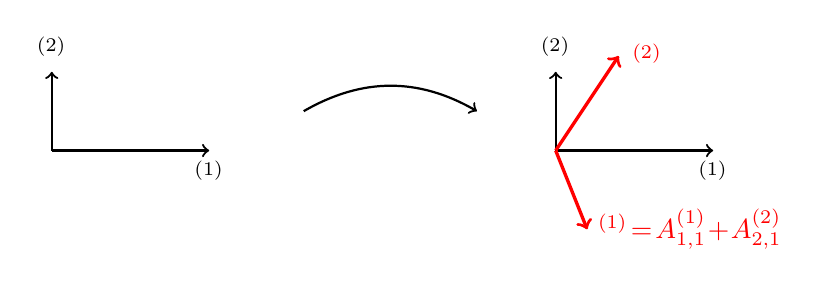
\begin{tikzpicture}[x=2cm]
      % LEFT: Standard basis vectors and unit square
      \begin{scope}
        \draw[->, thick] (0,0) -- (1,0) node[below] {$\vu^{(1)}$};
        \draw[->, thick] (0,0) -- (0,1) node[above] {$\vu^{(2)}$};
      \end{scope}
      % RIGHT: Transformed basis vectors and parallelogram
      \begin{scope}[shift={(3.2,0)}]
        \draw[->, thick] (0,0) -- (1,0) node[below] {$\vv^{(1)}$};
        \draw[->, thick] (0,0) -- (0,1) node[above] {$\vv^{(2)}$};
        \coordinate (A) at (0.2,-1.0);
        \coordinate (B) at (0.4,1.2);
        \draw[->, very thick, red] (0,0) -- (A) node[below,right] {$\mA \vu^{(1)}\!=\!A_{1,1}\vv^{(1)}\!+\!A_{2,1}\vv^{(2)}$};
        \draw[->, very thick, red] (0,0) -- (B) node[right,xshift=1pt] {$\mA \vu^{(2)}$};
      \end{scope}
      % Arrow between plots
      \draw[->, thick] (1.6,0.5) to[bend left] node[midway, above] {$\mA$} (2.7,0.5);
    \end{tikzpicture}
    \end{center}
    \caption{Eine Matrix $\mA$ definiert eine \gls{linearmap} zwischen zwei \glspl{vectorspace}. \label{fig_matrix_dict}} 
    \end{figure}
    Siehe auch: \gls{linearmap}, \gls{dataset}, \gls{linmodel}.},
  first={Matrix},
  firstplural={Matrizen},
  type=math,
  plural={Matrizen},
  text={Matrix}
}

\newglossaryentry{stratification}
{
  name={Stratifizierung},
  description={Stratifizierung bezeichnet den Prozess, ein \gls{dataset} in Teilmengen zu unterteilen, die als \glspl{stratum} bezeichnet werden, 
  entsprechend einem bestimmten Schlüsselkriterium \cite{oecd2008glossary,Everitt2010,OxfordStatisticsDictionary}.
Ziel dieses Vorgehens ist es sicherzustellen, dass eine \gls{ml}-Methode für jedes durch diese Attribute 
 definierte \gls{stratum} gute Leistungen erbringt. In einem medizinischen \gls{dataset} kann es zum Beispiel sinnvoll sein, 
 Patienten nach Altersgruppen zu stratifizieren, um die Leistungsfähigkeit eines \gls{ml}-\glsuseri{model} über alle Altersgruppen hinweg zu gewährleisten.  

  \begin{figure}[H]
  	\centering
	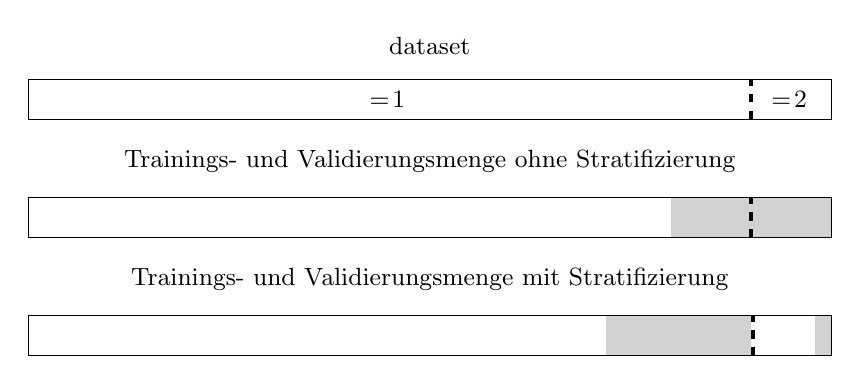
\begin{tikzpicture}[font=\small,x=1.7cm]
		\def\cellw{6.0}
		\def\cellh{0.5}
		\def\gap{1}
		\def\tfrac{0.8}
		\def\pA{0.9}
		\node[anchor=south] at (0.5*\cellw, \cellh+0.2) {\gls{dataset}};
		\node[anchor=south] at ({0.5*\cellw}, {-(\cellh+\gap)+\cellh+0.2}) {Trainings- und Validierungsmenge ohne Stratifizierung};
		\node[anchor=south] at (0.5*\cellw, {-2*(\cellh+\gap)+\cellh+0.2}) {Trainings- und Validierungsmenge mit Stratifizierung};
		\pgfmathsetmacro{\yDataset}{0}
		\pgfmathsetmacro{\yNoStrat}{-(\cellh+\gap)}
		\pgfmathsetmacro{\yStrat}{-2*(\cellh+\gap)}
		\pgfmathsetmacro{\xAB}{\pA*\cellw}
		\pgfmathsetmacro{\wA}{\pA*\cellw}
		\pgfmathsetmacro{\wB}{(1-\pA)*\cellw}
		\draw (0,\yDataset) rectangle ++(\cellw,\cellh);
		\draw[dashed,  line width=0.5mm] (\xAB,\yDataset) -- ++(0,\cellh);
		\node at (0.5*\wA, \yDataset+0.5*\cellh) {$\sensattr\!=\!1$};
		\node at ({\xAB+0.5*\wB}, {\yDataset+0.5*\cellh}) {$\sensattr\!=\!2$};
		\draw (0,\yNoStrat) rectangle ++(\cellw,\cellh);
		\pgfmathsetmacro{\xValStart}{\tfrac*\cellw}
		\pgfmathsetmacro{\valw}{(1-\tfrac)*\cellw}
		\fill[gray!35] (\xValStart,\yNoStrat) rectangle ++(\valw,\cellh);
		\draw[dashed,  line width=0.5mm] (\xAB,\yNoStrat) -- ++(0,\cellh);
		\draw (0,\yStrat) rectangle ++(\cellw,\cellh);
		\pgfmathsetmacro{\xAB}{\pA*\cellw}
		\draw[dashed, line width=1mm] (\xAB,\yStrat) -- ++(0,\cellh);
		\pgfmathsetmacro{\xAVal}{\tfrac*\wA}
		\pgfmathsetmacro{\wAVal}{(1-\tfrac)*\wA}
		\fill[gray!35] (\xAVal,\yStrat) rectangle ++(\wAVal,\cellh);
		\pgfmathsetmacro{\xBVal}{\xAB + \tfrac*\wB}
		\pgfmathsetmacro{\wBVal}{(1-\tfrac)*\wB}
		\fill[gray!35] (\xBVal,\yStrat) rectangle ++(\wBVal,\cellh);
	\end{tikzpicture}
  	\caption{Stratifizierung stellt sicher, dass sowohl die \gls{trainset} als auch die \gls{valset} ähnliche Verteilungen eines binären Schlüsselattributs $\sensattr$ aufweisen.}
  \end{figure}
  
  Wenn ein \gls{dataset} in eine \gls{trainset} und eine \gls{valset} aufgeteilt wird, sorgt die Stratifizierung dafür, dass beide Mengen
ähnliche Verteilungen des Schlüsselattributs enthalten. Ohne Stratifizierung kann eine kleine \gls{valset} die \glspl{datapoint} mit seltenen
 Attributen unterrepräsentieren oder vollständig ausschließen. Dies kann zu irreführenden Leistungsschätzungen führen.\\
  
  Siehe auch: \gls{validation}, \gls{kfoldcv}, \gls{stratum}.},
  text={Stratifizierung},
  first={Stratifizierung},
  plural={Stratifizierungen}
}

\newglossaryentry{stratum}
{
  name={Stratum},
  description={
Ein \index{Stratum} Stratum ist eine Teilmenge von \glspl{datapoint}, die alle eine gemeinsame Eigenschaft besitzen. Diese Eigenschaft kann entweder ein \gls{feature} oder ein \gls{label} sein. Zum Beispiel bilden in einem Wetter-\gls{dataset} alle Messungen von derselben \gls{fmi}-Wetterstation ein Stratum.\\[0.5em]
\begin{center}
\textbf{Beispiel (CSV-Ausschnitt):}\\
{\ttfamily
time,station,value,units\\
2023-06-01 12:00,Helsinki,18.2,degC\\
2023-06-01 13:00,Helsinki,18.5,degC\\
2023-06-01 14:00,Helsinki,19.0,degC\\
2023-06-01 12:00,Oulu,12.1,degC\\
2023-06-01 13:00,Oulu,12.4,degC\\
2023-06-01 14:00,Oulu,12.7,degC\\
2023-06-01 12:00,Tampere,15.3,degC\\
2023-06-01 13:00,Tampere,15.6,degC\\
2023-06-01 14:00,Tampere,16.0,degC
}
\end{center} 
Die Zeilen für jede Wetterstation (\texttt{Helsinki}, \texttt{Oulu}, \texttt{Tampere}) repräsentieren verschiedene Strata.\\
Siehe auch: \gls{stratification}, \gls{dataset}, \gls{datapoint}.},
  first={Stratum},
  firstplural={Strata},
  plural={Strata},
  text={Stratum}
}



\newglossaryentry{det}
{name={Determinante},
 description={Die \textbf{Determinante}\index{Determinante} $\det\,(\mA)$ einer quadratischen \gls{matrix} 
	$\mA = \big( \va^{(1)},\ldots, \va^{(\nrfeatures)} \big) \in \mathbb{R}^{\nrfeatures \times \nrfeatures}$ 
	ist eine \gls{funktion} ihrer Spaltenvektoren $\va^{(1)},\ldots,\va^{(\nrfeatures)} \in \mathbb{R}^{\nrfeatures}$ 
	\cite{DirschmidHansJorg1996TuF} mit folgenden Eigenschaften:
	\begin{itemize}
		\item \textbf{Normiert:} $$\det (\mI) = 1$$
		\item \textbf{Multilinear:}
		\begin{align} \nonumber
		\det \big(\va^{(1)},\ldots,\alpha\vu+ \beta \vv,\ldots,\va^{(\nrfeatures)} \big)
		&= \alpha\det \big(\va^{(1)},\ldots,\vu,\ldots,\va^{(\nrfeatures)} \big) \\
		&+ \beta\det \big(\va^{(1)},\ldots,\vv,\ldots,\va^{(\nrfeatures)} \big) \nonumber
		\end{align}
		\item \textbf{Antisymmetrisch:}
		$$\det \big(\ldots,\va^{(\featureidx)}, \ldots, \va^{(\featureidx')},\ldots \big) 
		= - \det \big(\ldots,\va^{(\featureidx')}, \ldots, \va^{(\featureidx)},\ldots \big).$$
	\end{itemize}
	
	Die \gls{matrix} $\mA$ kann als lineare Abbildung von $\mathbb{R}^{\nrfeatures}$ in sich selbst interpretiert werden. 
	Die Determinante $\det\,(\mA)$ charakterisiert, wie durch diese Abbildung orientierte Volumina in 
	$\mathbb{R}^{\nrfeatures}$ verändert werden \cite{GolubVanLoanBook}, \cite{Strang2007}. 
	
	Insbesondere gilt:
	\begin{itemize}
		\item $\det(\mA) > 0$: Orientierung wird beibehalten.
		\item $\det(\mA) < 0$: Orientierung wird umgekehrt.
		\item $\det(\mA) = 0$: Volumen kollabiert (nicht-invertierbar).
	\end{itemize}

	Zudem gilt: $\det(\mA \mB) = \det(\mA) \cdot \det(\mB)$ und falls $\mA$ diagonalisierbar mit Eigenwerten 
	$\eigval{1}, \ldots, \eigval{\nrfeatures}$ ist, dann ist
	$$\det(\mA) = \prod_{\featureidx=1}^{\nrfeatures} \eigval{\featureidx}$$
	\cite{HornMatAnalysis}.

	Für die Spezialfälle $\nrfeatures=2$ (2D) und $\nrfeatures=3$ (3D) lässt sich die Determinante als 
	orientierte Fläche bzw.\ Volumen interpretieren, das durch die Spaltenvektoren von $\mA$ aufgespannt wird.
	\begin{figure}[H]
		\centering
		\begin{tikzpicture}[x=2cm]
			\begin{scope}
				\draw[->, thick] (0,0) -- (1,0) node[below right] {$\vx$};
				\draw[->, thick] (0,0) -- (0,1) node[above left] {$\vy$};
			\end{scope}
			\begin{scope}[shift={(2.8,0)}]
				\coordinate (A) at (1.5,0.5);
				\coordinate (B) at (-0.2,1.2);
				\draw[->, very thick, red] (0,0) -- (A) node[below right] {$\mA \vx$};
				\draw[->, very thick, red] (0,0) -- (B) node[above left] {$\mA \vy$};
				\draw[fill=red!20, opacity=0.6] (0,0) -- (A) -- ($(A)+(B)$) -- (B) -- cycle;
				\draw[dashed] (A) -- ($(A)+(B)$);
				\draw[dashed] (B) -- ($(A)+(B)$);
				\node at (0.8,0.6) {\small $\det\,(\mA)$};
				\draw[->, thick, blue] (0.4,0.0) arc[start angle=0, end angle=35, radius=0.6];
			\end{scope}
			\draw[->, thick] (1.3,0.5) -- (2.4,0.5) node[midway, above] {$\mA$};
		\end{tikzpicture}
		\caption{Eine quadratische \gls{matrix} $\mA$ wirkt als lineare Abbildung auf $\mathbb{R}^{\nrfeatures}$. 
		Die Determinante beschreibt, wie dabei das orientierte Volumen verändert wird.}
	\end{figure}
	Siehe auch: \gls{eigenvalue}, \gls{inverse}.},
	first={Determinante},
	type=math,
	text={Determinante}
}

\newglossaryentry{hessian}
{name={Hesse-Matrix},
 	description={Betrachte\index{Hesse-Matrix} eine \gls{function} 
	$f: \mathbb{R}^{\nrfeatures} \to \mathbb{R}$, für die die partiellen Ableitungen 
	zweiter Ordnung an der Stelle $\featurevec'$ existieren. Dann ist die 
	Hesse-Matrix $\nabla^2 f(\featurevec')$ von $f$ an der Stelle $\featurevec'$ definiert 
	als die \gls{matrix} der partiellen Ableitungen zweiter Ordnung von $f$ an $\featurevec'$,
$$\nabla^{2} f(\featurevec') \;=\;
\begin{pmatrix}
\frac{\partial^{2} f}{\partial \feature_{1}^{2}}
& \frac{\partial^{2} f}{\partial \feature_{1}\, \partial \feature_{2}}
& \cdots
& \frac{\partial^{2} f}{\partial \feature_{1}\, \partial \feature_{\nrfeatures}} \\
\frac{\partial^{2} f}{\partial \feature_{2}\, \partial \feature_{1}}
& \frac{\partial^{2} f}{\partial \feature_{2}^{2}}
& \cdots
& \frac{\partial^{2} f}{\partial \feature_{2}\, \partial \feature_{\nrfeatures}} \\
\vdots & \vdots & \ddots & \vdots \\[1.2ex]
\frac{\partial^{2} f}{\partial \feature_{\nrfeatures}\, \partial \feature_{1}}
& \frac{\partial^{2} f}{\partial \feature_{\nrfeatures}\, \partial \feature_{2}}
& \cdots
& \frac{\partial^{2} f}{\partial \feature_{\nrfeatures}^{2}}
\end{pmatrix}.$$
Sind die partiellen Ableitungen zweiter Ordnung in einer \gls{neighborhood} um $\featurevec'$ 
\gls{continuous}, so ist die Hesse-Matrix symmetrisch, d.h.
$\frac{\partial^{2} f}{\partial \feature_{\featureidx}\, \partial \feature_{\featureidx'}} = 
\frac{\partial^{2} f}{\partial \feature_{\featureidx'}\, \partial \feature_{\featureidx}}$ für alle 
$\featureidx, \featureidx'$ \cite{RudinBookPrinciplesMatheAnalysis}. Ist $f$ zusätzlich 
\gls{convex}, so ist die Hesse-Matrix eine \gls{psd} \gls{matrix} \cite{BoydConvexBook}.
	\begin{figure}[H]
	\begin{center}
	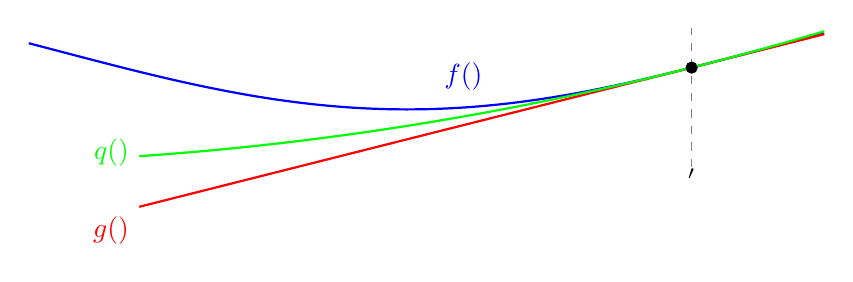
\begin{tikzpicture}[x=0.5cm]
		\begin{axis}[
			hide axis,
			xmin=3, xmax=6,
			ymin=0, ymax=6,
			domain=0:6,
			samples=100,
			width=10cm,
			height=6cm,
			clip=false
			]
		% Original nonlinear function h(x)
			\addplot[blue, thick, domain=3:6.6] {2 + sin(deg(x))} 
			node[pos=0.5, above right, yshift=3pt] {$f(\featurevec)$};
		% Tangent line as local linear approximation at x = 3
		% h(3) = 2 + sin(3), h'(3) = cos(3)
			\addplot[red, thick, domain=3.5:6.6] 
			{2 + sin(deg(6)) + cos(deg(6))*(x - 6)}
			node[pos=0, below left] {$g(\featurevec)$};
                %%%%%%%%%%%%%%%%%%%%%%%%%%%%%%%%%%%%%%%%%%%%%%%%
                \addplot[green, thick, domain=3.5:6.6]
                {2 + sin(deg(6)) + cos(deg(6))*(x - 6) - 0.5*sin(deg(6))*(x - 6)^2}
			node[pos=0, below left, yshift=10pt] {$q(\featurevec)$};
                %%%%%%%%%%%%%%%%%%%%%%%%%%%%%%%%%%%%%%%%%%%%%%%%
		% Mark point of approximation
			\addplot[mark=*] coordinates {(6, {2 + sin(deg(6))})};
			    % Vertical dashed line (ruler) at x = 3
			\addplot[dashed, gray] coordinates {(6,0) (6,2.4)};
			\node at (axis cs:6, -0.2) {$\featurevec'$};
			    % Plot the two points
			    % Coordinates of the two points
			\pgfmathsetmacro{\xA}{-1.5}
			\pgfmathsetmacro{\xB}{3}
			\pgfmathsetmacro{\yA}{2 + sin(deg(\xA))}
			\pgfmathsetmacro{\yB}{2 + sin(deg(\xB))}
		\end{axis}
		\vspace*{-10mm}
	\end{tikzpicture}
		\vspace*{-5mm}
	\end{center}
	\caption{
		Eine \gls{function} $f(\featurevec)$, die an einem Punkt $\featurevec'$ hinreichend 
		\gls{smooth} ist, kann lokal durch eine \gls{quadfunc} $q(\featurevec)$ approximiert werden, 
		die eine genauere Näherung als eine lineare \gls{function} $g(\featurevec)$ liefert. 
		\label{fig_quadapprox_hessian_dict}}
\end{figure}
		Die Hesse-Matrix $\nabla^2 f(\featurevec')$ kann verwendet werden, um eine 
		\gls{quadfunc}
		$$q(\featurevec) = (1/2) (\featurevec- \featurevec')^{T} \underbrace{\nabla^2 f(\featurevec')}_{\text{Hesse-Matrix}} 
		(\featurevec- \featurevec') +  (\featurevec- \featurevec')^{T} \underbrace{\nabla f(\featurevec')}_{\text{Gradient}} 
		+ f(\featurevec')$$
		zu berechnen, die $f$ lokal um $\featurevec'$ approximiert.\cite{MathematikOnline_HesseMatrix}
        		\\
		Siehe auch: \gls{differentiable}, \gls{matrix}, \gls{function}, \gls{quadfunc}. }, 
	first={Hesse-Matrix},
	type=math,
	text={Hesse-Matrix}
}

\newglossaryentry{continuous}
{name={stetig}, 
description={Eine \gls{function}\index{stetig} $f: \mathbb{R}^{\nrfeatures} \to \mathbb{R}$ heißt 
	stetig an einem Punkt $\featurevec' \in \mathbb{R}^{\nrfeatures}$, wenn für jedes 
	$\epsilon > 0$ ein $\delta > 0$ existiert, so dass für alle 
	$\featurevec \in \mathbb{R}^{\nrfeatures}$ mit 
	$\normgeneric{\featurevec - \featurevec'}{2} < \delta$ gilt: 
	$|f(\featurevec) - f(\featurevec')| < \epsilon$ \cite{RudinBookPrinciplesMatheAnalysis}. 
	Mit anderen Worten: Wir können $f(\featurevec)$ beliebig nahe an 
	$f(\featurevec')$ bringen, indem wir $\featurevec$ hinreichend nahe an 
	$\featurevec'$ wählen. Ist $f$ an jedem Punkt 
	$\featurevec' \in \mathbb{R}^{\nrfeatures}$ stetig, so heißt $f$ 
	stetig auf $\mathbb{R}^{\nrfeatures}$. 
	Der Begriff der stetigen \gls{function} lässt sich auf 
	\glspl{function} zwischen allgemeinen \gls{metric} Räumen 
	natürlich verallgemeinern \cite{RudinBookPrinciplesMatheAnalysis}.\\
		Siehe auch: \gls{euclidspace}, \gls{metric}.},
	first={stetig},
	type=math,
	text={stetig}
}


\newglossaryentry{linearmap}
{name={lineare Abbildung}, plural={lineare Abbildungen},
 description={Eine \textbf{lineare Abbildung}\index{lineare Abbildung} $f: \mathbb{R}^n \rightarrow \mathbb{R}^m$ 
	ist eine \gls{funktion}, die folgende Eigenschaften erfüllt:
	\begin{itemize}
		\item \textbf{Additivität:} $f(\vx + \vy) = f(\vx) + f(\vy)$
		\item \textbf{Homogenität:} $f(c\vx) = c f(\vx)$ für alle \glspl{vector} $\vx, \vy \in \mathbb{R}^n$ 
		und Skalare $c \in \mathbb{R}$
	\end{itemize}
	Daraus folgt insbesondere $f(\mathbf{0}) = \mathbf{0}$.
	Jede lineare \gls{map} kann als \gls{matrix}-Multiplikation dargestellt werden: 
	$$f(\vx) = \mA \vx \quad \text{für eine} \quad \mA \in \mathbb{R}^{m \times n}.$$

	Die Gesamtheit der reellwertigen linearen \glspl{map} eines gegebenen Eingaberaums bildet ein 
	\gls{linmodel}, das in vielen \glspl{ml}-Verfahren eingesetzt wird.
	\\
	Siehe auch: \gls{map}, \gls{funktion}, \gls{vector}, \gls{matrix}, \gls{linmodel}, \gls{ml}.},
	first={lineare Abbildung},
	text={lineare Abbildung}
}

\newglossaryentry{vector}
{name={Vektor},
	description={Ein \index{vector} Vektor ist ein Element eines \gls{vectorspace}. 
		In the context of \gls{ml}, a particularly important example of a \gls{vectorspace} 
		is the \gls{euclidspace} $\mathbb{R}^{\nrfeatures}$, where $\nrfeatures \in \mathbb{N}$ 
		is the (finite) dimension of the space. A vector $\vx \in \mathbb{R}^{\nrfeatures}$ 
		can be represented as a list or one-dimensional array of real numbers, i.e., 
		$x_1, \ldots, x_{\nrfeatures}$ with $x_\featureidx \in \mathbb{R}$ for 
		$\featureidx = 1, \ldots, \nrfeatures$. The value $x_\featureidx$ is the $\featureidx$-th 
		entry of the vector $\vx$. It can also be useful to view a vector $\vx \in \mathbb{R}^{\nrfeatures}$ 
		as a \gls{function} that maps each index $\featureidx \in \{1, \ldots, \nrfeatures\}$ 
		to a value $x_\featureidx \in \mathbb{R}$, i.e., $\vx: \featureidx \mapsto x_\featureidx$. 
		This perspective is particularly useful for the study of \glspl{kernelmethod}.
		\begin{figure}[H]
			% Left: Stem plot
			\begin{minipage}[c]{0.48\textwidth}
				\centering 
				2, -1, 3, 0, -2, 1
				\begin{minipage}{\textwidth}
				\vspace{5ex}
				\centering
				{\selectfont (a)}
				\end{minipage}
			\end{minipage}
			\hfill
			% Right: Column vector
			\begin{minipage}{0.48\textwidth}
			\centering
			\begin{tikzpicture}
			\begin{axis}[
    				width=6.5cm,
    				height=5cm,
    				title={},
    				xlabel={index $\featureidx$},
    				ylabel={$x_\featureidx$},
   		 		ymin=-3.5, ymax=3.5,
    				xmin=0.5, xmax=6.5,
   	 			xtick={1,2,3,4,5,6},
    				ytick={-3,-2,-1,0,1,2,3},
    				axis x line=bottom,        % <-- horizontal axis at y=0
    				axis y line=left,          % <-- vertical axis on the left
    				grid=both,
    				major grid style={dotted, gray!60},
    				enlargelimits=0.1
			]
			\addplot+[ycomb, thick, mark=*]
    			coordinates {
        				(1,2)
        				(2,-1)
       	 			(3,3)
        				(4,0)
        				(5,-2)
        				(6,1)
    			};
			\end{axis}
			\node at (2,-2.5) {(b)};
			\end{tikzpicture}
			\end{minipage}
			\caption{Two equivalent views of a vector $\vx= \big( 2, -1, 3, 0, -2, 1 \big)^{T} \in \mathbb{R}^{6}$.
			(a) As a numeric array. (b) As a \gls{map} $\featureidx \mapsto x_\featureidx$.}
			\label{fig:vector-function-dual_dict}
		\end{figure}
		See also: \gls{vectorspace}, \gls{euclidspace}, \gls{linearmap}.},
	first={vector},
	type=math,
	firstplural={vectors},
	plural={vectors},
	text={vector}
}


\newglossaryentry{vectorspace}
{name={vector space},
	description={A\index{vector space} \gls{vector} space $\mathcal{V}$ (also called linear space) 
	is a collection of elements, called \glspl{vector}, along with two operations: 
    addition (denoted by $\vv+\vw$) of two vectors $\vv,\vw$ and multiplication 
	(denoted $c\cdot \vv$) of a vector $\vv$ with a scalar $c$ who belongs to some 
	number field (a typical choice for this field is $\mathbb{R}$). The defining 
	property of a vector space is that it is closed under these operations, i.e.,
		\begin{itemize}
			\item If $\vv, \vw \in \mathcal{V}$, then $\vv + \vw \in \mathcal{V}$.
			\item If $\vv \in \mathcal{V}$ and $c \in \mathbb{R}$, then $c \vv \in \mathcal{V}$.
			\item In particular, $\mathbf{0} \in \mathcal{V}$.
		\end{itemize}
		\begin{figure}[ht]
		\centering
			\begin{tikzpicture}[>=Stealth, scale=1.2]
				  % Coordinates
  			\coordinate (O) at (0,0);            % Origin
  			\coordinate (V) at (2,1.5);          % vector v
  			\coordinate (W) at (1,3);            % vector w
  			\coordinate (VplusW) at (3,4.5);     % v + w
  			\coordinate (HalfV) at (1,0.75);     % 0.5 * v
  			\draw[->, thick, blue] (O) -- (V) node[pos=1, right] {$\vv$};
  			\draw[->, thick, red] (O) -- (W) node[pos=1, left] {$\vw$};
  			\draw[->, thick, purple] (O) -- (VplusW) node[pos=0.99, above right] {$\vv+\vw$};
  			\draw[dashed, red] (V) -- (VplusW);
  			\draw[dashed, blue] (W) -- (VplusW);
  			\draw[->, thick, orange] (O) -- (HalfV) node[midway, right] {$0.5\vv$};
			% Filled dots
  			\filldraw[black] (O) circle (2pt) node[below left] {$\mathbf{0}$};  % origin
  			\filldraw[blue] (V) circle (2pt);         % v
  			\filldraw[red] (W) circle (2pt);          % w
  			\filldraw[purple] (VplusW) circle (2pt);  % v + w
  			\filldraw[orange] (HalfV) circle (2pt);   % 0.5v
			\end{tikzpicture}
			\caption{A vector space $\mathcal{V}$ is a collection of vectors such that scaling 
			and adding them always yields another vector in $\mathcal{V}$. In \gls{ml} applications, 
			 vectors are used to represent \glspl{datapoint} (or their \glspl{featurevec}) and 
			 invariances (or symmetries) of \glspl{model}.}
			\label{fig:vector-ops_dict}
		\end{figure}
		A common example of a vector space is the \gls{euclidspace} $\mathbb{R}^n$, which is widely used in 
		\gls{ml} to represent \glspl{model} and \glspl{dataset}.
		\\
		See also: \gls{vector}, \gls{euclidspace}, \gls{linmodel}, \gls{linearmap}.},
	first={vector space},
	type=math,
	text={vector space}
}


\newglossaryentry{stochastic}
{name={stochastic},
	description={We refer to a \index{stochastic} method as stochastic if it involves a 
		random component or is governed by probabilistic laws. \Gls{ml} methods use randomness 
		to reduce computational complexity (e.g., see \gls{stochGD}) or 
		to capture \gls{uncertainty} in \glspl{probmodel}.
		\\
		See also: \gls{stochGD}, \gls{uncertainty}, \gls{probmodel}.},
	first={stochastic},
	text={stochastic}
}

\newglossaryentry{stochproc}
{name={stochastic process},
	description={
		A \gls{stochastic} process\index{stochastic process} is a collection of 
		\glspl{rv} defined on a common \gls{probspace}, indexed by some set 
		$\mathcal{I}$ \cite{papoulis,GrayProbBook,Brockwell91}. The index set 
		$\mathcal{I}$ typically represents time or space, allowing to represent 
		random phenomena that evolve across time or spatial dimensions—for example, 
		sensor noise or financial time series. Stochastic processes are not limited 
		to temporal or spatial settings. For instance, random \glspl{graph} such as 
		the \gls{ergraph} or the \gls{sbm} 
		can also be viewed as stochastic processes. Here, the index set $\mathcal{I}$ 
		consists of node pairs that index \glspl{rv} whose values encode 
		the presence or weight of an edge between two nodes. Moreover, \gls{stochastic} 
		processes naturally arise in the analysis of \glspl{stochalgorithm}, 
		such as \gls{stochGD}, which construct a sequence of \glspl{rv}. 
		\\
		See also:  \gls{rv}, \gls{sbm}, \gls{stochGD}, \gls{uncertainty}, \gls{probmodel}.},
	first={stochastic process},
	firstplural={stochastic processes},
	plural={stochastic processes},
	text={stochastic process}
}

\newglossaryentry{characteristicfunc}
{name={characteristic function},
	description={The characteristic \gls{function}\index{characteristic function} 
		of a real-valued \gls{rv} $x$ is the \gls{function} \cite[Sec. 26]{BillingsleyProbMeasure}
		$$ \phi_{x}(t) \defeq \expect { \exp\,(j t x) } \mbox{ with } j = \sqrt{-1}.$$
	 	The characteristic \gls{function} uniquely determines the \gls{probdist} of $x$. 
		\\
		See also: \gls{rv}, \gls{probdist}.},
	first={characteristic function},
	firstplural={characteristic functions}, 
	plural={characteristic functions},
	text={characteristic function}
}

\newglossaryentry{entropy}
{name={entropy},
	description={Entropy\index{entropy} quantifies the \gls{uncertainty} or unpredictability associated with an \gls{rv} \cite{coverthomas}. 
		For a discrete \gls{rv} $x$ taking on values in a finite set $\mathcal{S} = \{x_1, \ldots, x_n\}$ with 
		a \gls{probability} mass \gls{function} $p_i \defeq \prob{x = x_i}$, the entropy is defined as
		\[
		H(x) \defeq -\sum_{i=1}^n p_i \log p_i.
		\]
		Entropy is maximized when all outcomes are equally likely, and minimized (i.e., zero) 
		when the outcome is deterministic. A \gls{generalization} of the concept of entropy for continuous 
		\glspl{rv} is \gls{diffentropy}. 
		\\
		See also: \gls{uncertainty}, \gls{probmodel}.},
	first={entropy},
	text={entropy}
}

\newglossaryentry{diffentropy}
{name={differential entropy},
	description={For\index{differential entropy} a real-valued \gls{rv} $\featurevec \in \mathbb{R}^{\nrfeatures}$ 
		with a \gls{pdf} $p(x)$, the differential \gls{entropy} is defined as \cite{coverthomas}
		\[
		h(\featurevec) \defeq - \int p(\featurevec) \log p(\featurevec) \, d\featurevec.
		\]
		Differential \gls{entropy} can be negative and lacks some properties of \gls{entropy} for 
		discrete-valued \glspl{rv}, such as invariance under a change of variables \cite{coverthomas}. 
		Among all \glspl{rv} with a given \gls{mean} $\meanvecgeneric$ and \gls{covmtx} $\covmtxgeneric$, 
		$h(\featurevec)$ is maximized by $\featurevec \sim \mvnormal{\meanvecgeneric}{\covmtxgeneric}$. 
		\\
		See also: \gls{uncertainty}, \gls{probmodel}.},
	first={differential entropy},
	text={differential entropy}
}

	\newglossaryentry{minimum}
{name=Minimum,
 description={Bei einer gegebenen Menge and reeller Zahlen, ist das Minimum \index{minimum} das kleinste dieser Zahlen.},
 first={Minimum},text={Minimum}, plural={Minima}
}

\newglossaryentry{co-domain}
{name={Zielmenge}, 
	description={Die Zielmenge\index{Zielmenge} einer \gls{function} 
	$f: \mathcal{U} \rightarrow \mathcal{V}$ ist die Menge $\mathcal{V}$, 
	in die $f$ die Elemente ihres Definitionsbereichs $\mathcal{U}$ abbildet.  
	\\
	Siehe auch: \gls{function}, \gls{domain}, \gls{map}.},
	first={Zielmenge},
	firstplural={Zielmengen}, 
	type=math, 
	plural={Zielmengen},
	text={Zielmenge}
}

\newglossaryentry{domain}
{name={Definitionsbereich}, 
	description={Der Definitionsbereich\index{Definitionsbereich} einer \gls{function} 
	$f: \mathcal{U} \rightarrow \mathcal{V}$ ist die Menge $\mathcal{U}$, 
	aus der $f$ seine Eingaben nimmt.  
	\\
	Siehe auch: \gls{function}, \gls{co-domain}, \gls{map}.},
	first={Definitionsbereich},
	firstplural={Definitionsbereiche}, 
	type=math, 
	plural={Definitionsbereiche},
	text={Definitionsbereich}
}


\newglossaryentry{function}
{name={Funktion}, 
	description={Eine Funktion\index{Funktion} zwischen zwei Mengen $\mathcal{U}$ und $\mathcal{V}$ ordnet  
	jedem Element $u \in \mathcal{U}$ genau ein Element $f(u) \in \mathcal{V}$ zu \cite{RudinBookPrinciplesMatheAnalysis}.
	Wir schreiben dies als 
	$$f: \mathcal{U} \rightarrow \mathcal{V}: u \mapsto f(u)$$ 
	wobei $\mathcal{U}$ der \gls{domain} und $\mathcal{V}$ der \gls{co-domain} von $f$ entspricht. 
	Das heißt, eine Funktion $f$ definiert für jedes Eingabeelement $u \in \mathcal{U}$ genau ein Ausgabeelement $f(u) \in \mathcal{V}$ (siehe Abb. \ref{fig_function_dict}).
	\begin{figure}[H]
		\centering
		\begin{tikzpicture}[>=stealth, node distance=1.2cm and 2.5cm]
			\tikzset{dot/.style={circle, fill=black, inner sep=1.2pt}}
			\node (A) [dot, label=left:$a$] {};
			\node (B) [dot, below=of A, label=left:$b$] {};
			\node (C) [dot, below=of B, label=left:$c$] {};
			\node (1) [dot, right=4cm of A, label=right:$\star$] {};
			\node (2) [dot, below=of 1, label=right:$\circ$] {};
			\node (3) [dot, below=of 2, label=right:$\otimes$] {};
			\node[draw=blue!70, thick, ellipse, inner sep=0.5cm, fit=(A)(B)(C), label=above:$\mathcal{U}$] {};
			\node[draw=green!70!black, thick, ellipse, inner sep=0.5cm, fit=(1)(2)(3), label=above:$\mathcal{V}$] {};
			\draw[->] (A) -- (2);
			\draw[->] (B) -- (1);
			\draw[->] (C) -- (2);
		\end{tikzpicture}
		\caption{Eine Funktion \( f \colon \mathcal{U} \to \mathcal{V} \), die jedes Element 
		des \gls{domain} $\mathcal{U} =  \{a,b,c\}$ genau einem Element der 
		\gls{co-domain} $\mathcal{V} = \{\star,\circ,\otimes\}$ zuordnet. \label{fig_function_dict}}
	\end{figure}},
	first={Funktion},
	firstplural={Funktionen}, 
	type=math, 
	plural={Funktionen},
	text={Funktion}
}



\newglossaryentry{map}
{name={map}, 
	description={We\index{map} use the term map as a synonym for \gls{function}.
		\\
		See also: \gls{function}.},
	first={map},
	firstplural={maps},	
	plural={maps},
	text={map}
}

\newglossaryentry{attention}
{name={attention}, 
	description={In einigen \gls{ml}-Anwendungen\index{attention} bestehen \glspl{datapoint} 
	aus kleineren Einheiten, die als \glspl{token} bezeichnet werden. Zum Beispiel besteht ein Satz 
	aus Wörtern, ein Bild aus Pixel-Patches und ein Netzwerk aus Knoten. Im Allgemeinen 
	sind die \glspl{token}, die einen einzelnen \gls{datapoint} bilden, nicht voneinander unabhängig. 
	Stattdessen hängt jedes \gls{token} eines \gls{datapoint} von bestimmten anderen \glspl{token} ab 
	(beziehungsweise "pay attention" auf sie). \Glspl{probmodel} bieten einen prinzipiellen Rahmen, um 
	solche Abhängigkeiten darzustellen und zu analysieren \cite{Blei2003}. Attention-Mechanismen verfolgen 
	einen direkteren Ansatz ohne explizite Bezugnahme auf ein \gls{probmodel}. Die Grundidee besteht darin, 
	die Beziehung zwischen zwei Tokens $\nodeidx$ und $\nodeidx'$ mittels einer parametrisierten 
	\gls{function} $f^{(\weights)}(\nodeidx,\nodeidx')$ darzustellen, wobei die \glspl{parameter} 
	$\weights$ über eine Variante von \gls{erm} gelernt werden. Praktische Attention-Mechanismen 
	unterscheiden sich in der genauen Wahl des Attention-\gls{model} $f^{(\weights)}(\nodeidx,\nodeidx')$ 
	sowie der verwendeten \gls{erm}-Variante. Eine weit verbreitete Familie von Attention-Mechanismen 
	definiert die \glspl{parameter} $\weights$ in Form von zwei \glspl{vector}, die jedem Token $\nodeidx$ 
	zugeordnet sind, nämlich einem Query-\gls{vector} $\vq^{(\nodeidx)}$ und einem Key-\gls{vector} $\vk^{(\nodeidx')}$. 
	Für ein gegebenes Token $\nodeidx$ mit Query $\vq^{(\nodeidx)}$ und ein anderes Token $\nodeidx'$ mit Key 
	$\vk^{(\nodeidx')}$ quantifiziert die Größe 
	$\big( \vq^{(\nodeidx)} \big)^{\top} \vk^{(\nodeidx')}$, in welchem Ausmaß Token $\nodeidx$ auf 
	Token $\nodeidx'$ "attentiert" bzw. von ihm abhängt (siehe Abb. \ref{fig_attention_dict}).
	\begin{figure}[H]
		\centering
		\begin{tikzpicture}[>=stealth, node distance=0.2cm and 0.2cm,
		every node/.style={inner sep=2pt, font=\large}, baseline]
		% Words (sentence: All human beings are born free and equal.)
		\node (w1) [draw, fill=gray!10, rounded corners] {All};
		\node (w2) [draw, fill=gray!10, right=of w1, rounded corners] {human};
		\node (w3) [draw, fill=gray!10, right=of w2, rounded corners] {beings};
		\node (w4) [draw, fill=gray!10, right=of w3, rounded corners] {are};
		\node (w5) [draw, fill=gray!10, right=of w4, rounded corners] {born};
		\node (w6) [draw, fill=gray!10, right=of w5, rounded corners] {free};
		\node (w7) [draw, fill=gray!10, right=of w6, rounded corners] {and};
		\node (w8) [draw, fill=blue!20, right=of w7, rounded corners] {equal};
		\node[font=\footnotesize, below=0.15cm of w8, align=center] (labeli) {$\nodeidx$ \\ $\vq^{(\nodeidx)},\ \vk^{(\nodeidx)}$};
		\node[font=\footnotesize, below=0.15cm of w1, align=center] (labelii) {$\nodeidx'$ \\ $\vq^{(\nodeidx')},\ \vk^{(\nodeidx')}$};
		\node (eqTop) [above=1.8cm of w8] {};
		\draw[->, thick, opacity=0.3] (w8.north) .. controls +(up:1.0cm) and +(up:1.0cm) .. (w6.north);
		\draw[->, thick, opacity=0.3] (w8.north) .. controls +(up:1.2cm) and +(up:1.0cm) .. (w5.north);
		\draw[->, thick, opacity=1]  (w8.north)  .. controls +(up:1.8cm) and +(up:1.0cm) ..  node[midway, text=black, above] {$f^{(\weights)}(\nodeidx,\nodeidx')$}  (w1.north);
		\end{tikzpicture}
		\caption{Attention-Mechanismen lernen eine parametrisierte \gls{function} $f^{(\weights)}(\nodeidx,\nodeidx')$, um zu messen, 
		wie stark Token $\nodeidx$ auf Token $\nodeidx'$ "attentiert". Eine weit verbreitete Konstruktion von 
		$f^{(\weights)}(\nodeidx,\nodeidx')$ nutzt Query- und Key-\glspl{vector}, bezeichnet durch 
		$\vq^{(\nodeidx)}$ und $\vk^{(\nodeidx)}$, die jedem Token $\nodeidx$ zugeordnet werden \cite{vaswani2017attention}. 
		\label{fig_attention_dict}}
	\end{figure}
	See also: \gls{function}, \gls{nlp}, \gls{token}.},
	first={attention},
	text={attention}
}

\newglossaryentry{transformer}
{name={transformer},
 description={Im Kontext von \gls{ml} bezeichnet der Begriff transformer\index{transformer} 
 	ein \glspl{ann}, das eine Form von \gls{attention}-Mechanismus verwendet, 
 	um Abhängigkeiten zwischen \glspl{token} zu erfassen \cite{vaswani2017attention}. 
 	Der \gls{attention}-Mechanismus unterscheidet Transformer von früheren 
	\glspl{model}, die für sequentielle \gls{data}, wie z. B. \glspl{rnn}, eingesetzt wurden. 
	Ein Transformer-\gls{ann} kombiniert häufig mehrere \gls{attention}-\glspl{layer}, 
	die über traditionelle \gls{layer}-Architekturen integriert werden.\\
	See also: \gls{nlp}, \gls{attention}.
  }, 
 first = {transformer}, 
 text={transformer},
 firstplural={transformers}, 
 plural = {transformers}
}

\newglossaryentry{rnn}
{name={recurrent neural network (RNN)},
 description={Ein \index{recurrent neural network (RNN)} RNN 
 	ist ein spezieller Typ eines \gls{ann}, der für die Verarbeitung von 
 	\gls{data} entwickelt wurde, die als Sequenz von \glspl{token} vorliegt. 
 	Ein RNN besitzt einen internen Hidden-State, der bei der Verarbeitung neuer 
 	\glspl{token} rekurrent aktualisiert wird. Durch diese rekurrente Struktur kann 
 	Information über verschiedene Zeitschritte hinweg propagiert werden, wodurch 
 	RNNs für Aufgaben wie Spracherkennung, Sprachmodellierung oder Zeitreihenprognose 
 	besonders geeignet sind. 
 	Die sequentielle Berechnung begrenzt jedoch die Parallelisierbarkeit und 
 	erhöht die Komplexität bei der Anwendung von \glspl{gdmethod}. Varianten wie 
 	Long Short-Term Memory (LSTM) und Gated Recurrent Unit (GRU) 
 	adressieren diese Einschränkungen, indem sie den Informationsfluss 
 	über längere Zeiträume stabilisieren.}, 
 first = {recurrent neural network (RNN)},
 text={RNN}
}

\newglossaryentry{llm}
{name={large language model (LLM)},
 description={A\index{large language model (LLM)} LLM is an umbrella term for \gls{ml} 
               methods that use high-dimensional \gls{ml} \glspl{model} (with billions 
			   of \glspl{modelparam}) trained on large collections of text \gls{data}. 
 			  LLMs are used to analyze or generate sequences of \glspl{token} which 
               constitute text \gls{data}. Many current LLMs use some variant of 
			   a \gls{transformer} that is trained via self-supervised learning:  
			   The training is based on the task of predicting a few words that 
			   are intentionally removed from a large text corpus. Thus, we can 
			   construct \glspl{labeled datapoint} simply by selecting some words 
			   from a given text as \glspl{label} and the remaining words as \glspl{feature} 
			   of \glspl{datapoint}. This construction requires 
		       very little human supervision and allows for generating sufficiently 
		       large \glspl{trainset} for LLMs.\\ 
			   See also: \gls{nlp}, \gls{token}, \gls{transformer}.}, 
  first = {LLM}, 
  firstplural={LLMs}, 
  text = {LLM}, 
  plural = {LLMs} 
}

\newglossaryentry{selfsupervisedlearning}
{name={selbstüberwachtes Lernen},
 description={Selbstüberwachtes Lernen \index{selbstüberwachtes Lernen} verwendet einen Teil 
 	der \glspl{feature} eines \gls{datapoint} als \gls{label}. Zum Beispiel kann, 
 	wenn ein \gls{datapoint} aus einem Satz innerhalb eines Textdokuments besteht, 
 	das letzte Wort des Satzes als \gls{label} verwendet werden, das aus allen 
 	vorhergehenden Wörtern vorhergesagt werden soll (die die \glspl{feature} des 
 	\gls{datapoint} bilden). Eine Hauptanwendung des selbstüberwachten Lernens 
 	liegt im Bereich der \gls{nlp} für das Training von \glspl{llm} auf Basis großer 
 	Textsammlungen.\\
 	See also: \gls{feature}, \gls{label}, \gls{llm}.}, 
 first = {selbstüberwachtes Lernen}, 
 text = {selbstüberwachtes Lernen}
}


\newglossaryentry{optproblem}
{name={optimization problem}, 
	description={An\index{optimization problem} optimization problem is a mathematical 
		   structure consisting of an \gls{objfunc} $f: \mathcal{U} \rightarrow \mathcal{V}$ 
		   defined over an optimization variable $\weights \in \mathcal{U}$, together with a 
		   feasible set $\mathcal{W} \subseteq \mathcal{U}$. The co-domain $\mathcal{V}$ is 
		   assumed to be ordered, meaning that for any two elements $\mathbf{a}, \mathbf{b} \in \mathcal{V}$, 
		   we can determine whether $\mathbf{a} < \mathbf{b}$, $\mathbf{a} = \mathbf{b}$, 
		   or $\mathbf{a} > \mathbf{b}$. The goal of optimization is to find those values $\weights \in \mathcal{W}$ 
		   for which the objective $f(\weights)$ is extremal—i.e., minimal or maximal \cite{BoydConvexBook}, \cite{BertsekasNonLinProgr}, \cite{nesterov04}.
		   \\
		   See also: \gls{objfunc}.},
	first={optimization problem},
	firstplural={optimization problems}, 
	plural={optimization problems}, 
	text={optimization problem}
}

\newglossaryentry{optmethod}
{name={optimization method},
	description={An\index{optimization method} optimization method is an \gls{algorithm} that 
		reads in a representation of an \gls{optproblem} and delivers an (approximate) solution 
		as its output \cite{BoydConvexBook}, \cite{BertsekasNonLinProgr}, \cite{nesterov04}.
		 \\
		 See also: \gls{algorithm}, \gls{optproblem}.},
	first={optimization method},
	firstplural={optimization methods}, 
	plural={optimization methods}, 
	text={optimization method}
}

\newglossaryentry{convexopt} {
    name={konvexe Optimierung},
    description={Die konvexe Optimierung\index{konvexe Optimierung} beschäftigt sich mit der Formulierung, den Eigenschaften und effizienten Lösungsmethoden für \gls{convex} \glspl{optproblem} \cite{BoydConvexBook}. Ein \gls{convex} \gls{optproblem} (definiert auf dem \gls{euclidspace} $\mathbb{R}^{\nrfeatures}$) besteht aus einer \gls{convex} \gls{objfunc} $f: \mathbb{R}^{\nrfeatures} \rightarrow \mathbb{R}$ und einer \gls{convex} zulässigen Menge $\mathcal{C}$ für die Optimierungsvariable $\weights$. Es kann kompakt geschrieben werden als \cite{BoydConvexBook} 
    $$
    \min_{\weights \in \mathcal{C}} f(\weights).
    $$
    Alternativ kann ein \gls{convex} \gls{optproblem} in Form von \gls{convex}en Nebenbedingungsfunktionen $g_1,\ldots,g_k$ ausgedrückt werden:
    \begin{align}
    \min_{\weights \in \mathbb{R}^{\nrfeatures}} & f(\weights) \nonumber \\
    \text{s.d.} \quad & g_{\sampleidx}(\weights) \leq 0, \quad \sampleidx=1,\,\ldots,\,k. \label{equ_def_convx_opt_constr_dict}
    \end{align}
    \begin{figure}
    \centering
    \begin{tikzpicture}[>=stealth, scale=1.0]
    % Achsen
    \draw[->] (-3,0) -- (5.2,0) node[below] {$\vc$};
    \draw[->] (0,-0.2) -- (0,4.2) node[left] {$t$};

    % Exponentielle Grenze: t = 3 e^{-g}
    \draw[thick, domain=-1:3, smooth, variable=\x, name path=boundary] plot ({\x},{exp(-\x)});

    % Transparente Epigraphregion (oberhalb der Kurve)
    \path[fill=gray!40, opacity=0.4] (-1,3) -- (-1,{exp(1)}) -- plot[domain=-1:3] ({\x},{exp(-\x)}) -- (3,3) -- cycle;

    % Schnittpunkt mit vertikaler Achse (g=0): markieren und f^* beschriften
    \fill (0,1) circle (1.6pt) node[left] {$f^{\ast}$};

    % Tangente bei g=1: Steigung = -e^{-1}, durch (1, e^{-1})
    \draw[dashed, domain=-1:3, smooth, variable=\x] plot ({\x},{(2/exp(1)) - (1/exp(1))*\x});

    % Punkt der Tangente markieren
    \fill (1,{1/exp(1)}) circle (1.2pt);

    % Beschriftung der schattierten Region
    \node at (2.6,2.5) {$\mathcal{A}$};
    \node [below,yshift=-3pt] at (0,-0.2) {$\mathbf{0}$};
    \end{tikzpicture}
    \caption{Ein \gls{convex} \gls{optproblem} \eqref{equ_def_convx_opt_constr_dict} kann durch eine Menge $\mathcal{A}$ dargestellt werden,
	 die aus den erreichbaren Zielwerten $t$ und den Nebenbedingungswerten $\vc=\big(c_{1},\ldots,c_{\nrfeatures}\big)^{T}$ besteht, 
	 d.h., $f(\weights) \leq t, g_{1}(\weights)\leq c_{1},\ldots, g_{k}(\weights) \leq c_{k}$ für ein $\weights \in \mathbb{R}^{\nrfeatures}$.
	 Der optimale Wert $f^{\ast}$ des \gls{optproblem} ist der kleinste $t$, für den $(\mathbf{0},t) \in \mathcal{A}$ gilt.}
    \end{figure}

    Die Formulierung \eqref{equ_def_convx_opt_constr_dict} führt zur Epigraphform \cite[Sec 5.3]{BoydConvexBook}:
    $$
    \inf \big\{ t \in \mathbb{R} : (\mathbf{0}, t) \in \mathcal{A} \big\},
    $$
    mit der Menge
    \begin{align}
    \mathcal{A} \defeq \big\{ (\vc,t) & \in \mathbb{R}^{\nrfeatures} \times \mathbb{R} : f(\weights) \leq t, \, \nonumber \\
    & g_{\sampleidx}(\weights) \leq c_{\sampleidx}, \, \sampleidx = 1,\ldots,k, \text{ für ein } \weights \in \mathbb{R}^{\nrfeatures} \big\}. \nonumber
    \end{align}
    Es kann gezeigt werden, dass, da $f,g_{1},\ldots,g_{k}$ \gls{convex}e \glspl{function} sind, $\mathcal{A}$ eine \gls{convex}e Menge ist \cite[Ch.2]{BoydConvexBook}.
	 Die Menge $\mathcal{A}$ charakterisiert vollständig das \gls{optproblem}~\eqref{equ_def_convx_opt_constr_dict} und kann als \gls{epigraph} der \gls{objfunc}~$f$ eingeschränkt 
	 auf die zulässige Region, definiert durch die Nebenbedingungsfunktionen $g_1,\ldots,g_k$, interpretiert werden.\\
    Siehe auch: \gls{convex}, \gls{optproblem}, \gls{optmethod}.
    },
    first={konvexe Optimierung},
    type=math,
    text={konvexe Optimierung}
}

\newglossaryentry{newtonmethod}{
    name={Newton-Verfahren},
    description={Das Newton-Verfahren\index{Newton-Verfahren} ist ein iteratives \gls{optmethod}, um lokale \glspl{minimum} oder \glspl{maximum} einer \gls{differentiable} \gls{objfunc} $f(\weights)$ zu finden. 
    Ähnlich wie bei \glspl{gdmethod} wird beim Newton-Verfahren eine neue Schätzung $\estparams{\iteridx+1}$ durch Optimierung einer lokalen Näherung von $f(\weights)$ um die aktuelle Schätzung $\estparams{\iteridx}$ berechnet. 
    Im Gegensatz zu \glspl{gdmethod}, die den \gls{gradient} verwenden, um eine lokale lineare Näherung zu bilden, nutzt das Newton-Verfahren die \gls{hessian} \gls{matrix}, um eine lokale quadratische Näherung zu erstellen. 
    Insbesondere wird ab einer Anfangsschätzung $\estparams{0}$ die Schätzung iterativ nach
    \[
    \estparams{\iteridx+1}= \estparams{\iteridx}- \big( \nabla^2 f\big(\estparams{\iteridx}\big) \big)^{-1} \nabla f\big( \estparams{\iteridx} \big), \quad \iteridx=0,\,1,\,\ldots,
    \]
    aktualisiert. Hierbei bezeichnet $\nabla f\big(\estparams{\iteridx} \big)$ den \gls{gradient} und $\nabla^2 f(\weights^{(\iteridx)})$ die \gls{hessian} der \gls{objfunc} $f$. Da die Verwendung einer \gls{quadfunc} als lokale Näherung präziser ist als die lineare Näherung (die ein Spezialfall einer \gls{quadfunc} darstellt), konvergiert das Newton-Verfahren in der Regel schneller als \glspl{gdmethod} (vgl. Abb. \ref{fig_newtonmethod_dict}). 
    Diese schnellere \gls{convergence} geht jedoch mit einem höheren Rechenaufwand der Iterationen einher, da jede Iteration die Inversion der \gls{hessian} erfordert. 
    \begin{figure}[H]
    \centering
    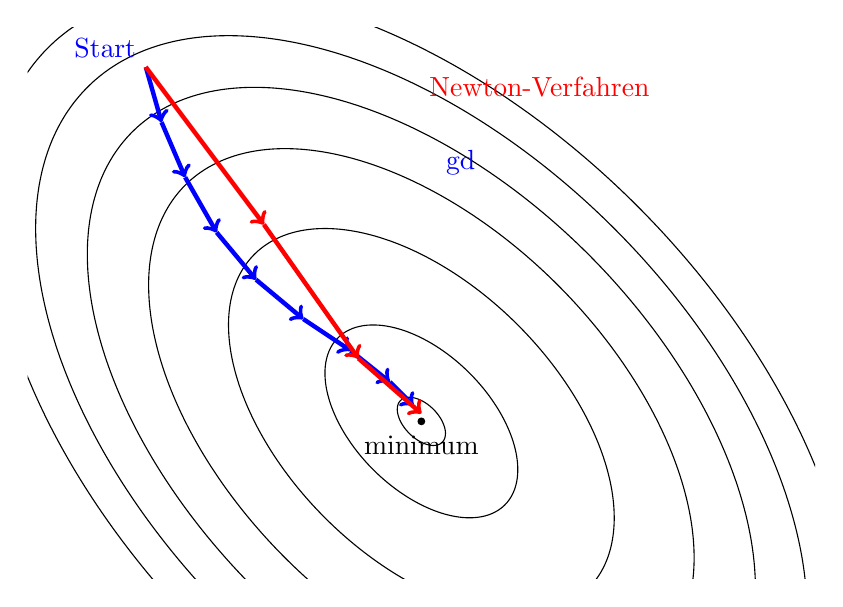
\begin{tikzpicture}[samples=200,smooth]
        \begin{scope}
            \clip(-5,-2) rectangle (5,5);
            % Konturen der Funktion
            \draw[thin] plot[domain=0:360] ({1.5*cos(\x)*sqrt(20/(sin(2*\x)+2))},{1.5*sin(\x)*sqrt(20/(sin(2*\x)+2))});
            \draw[thin] plot[domain=0:360] ({1.5*cos(\x)*sqrt(16/(sin(2*\x)+2))},{1.5*sin(\x)*sqrt(16/(sin(2*\x)+2))});
            \draw[thin] plot[domain=0:360] ({1.5*cos(\x)*sqrt(12/(sin(2*\x)+2))},{1.5*sin(\x)*sqrt(12/(sin(2*\x)+2))});
            \draw[thin] plot[domain=0:360] ({1.5*cos(\x)*sqrt(8/(sin(2*\x)+2))},{1.5*sin(\x)*sqrt(8/(sin(2*\x)+2))});
            \draw[thin] plot[domain=0:360] ({1.5*cos(\x)*sqrt(4/(sin(2*\x)+2))},{1.5*sin(\x)*sqrt(4/(sin(2*\x)+2))});
            \draw[thin] plot[domain=0:360] ({1.5*cos(\x)*sqrt(1/(sin(2*\x)+2))},{1.5*sin(\x)*sqrt(1/(sin(2*\x)+2))});
            \draw[thin] plot[domain=0:360] ({1.5*cos(\x)*sqrt(0.0625/(sin(2*\x)+2))},{1.5*sin(\x)*sqrt(0.0625/(sin(2*\x)+2))});
            % Gradient Descent-Pfad
            \draw[->,blue,ultra thick] (-3.5,4.5) -- (-3.3,3.8);
            \draw[->,blue,ultra thick] (-3.3,3.8) -- (-3,3.1);
            \draw[->,blue,ultra thick] (-3,3.1) -- (-2.6,2.4);
            \draw[->,blue,ultra thick] (-2.6,2.4) -- (-2.1,1.8);
            \draw[->,blue,ultra thick] (-2.1,1.8) -- (-1.5,1.3);
            \draw[->,blue,ultra thick] (-1.5,1.3) -- (-0.9,0.9);
            \draw[->,blue,ultra thick] (-0.9,0.9) -- (-0.4,0.5);
            \draw[->,blue,ultra thick] (-0.4,0.5) -- (-0.1,0.2);
            \node[blue,above left] at (-3.5,4.5) {Start};
            \node[blue,above] at (0.5,3) {\gls{gd}};
            % Newton-Verfahren-Pfad
            \draw[->,red,ultra thick] (-3.5,4.5) -- (-2,2.5);
            \draw[->,red,ultra thick] (-2,2.5) -- (-0.8,0.8);
            \draw[->,red,ultra thick] (-0.8,0.8) -- (0,0.1);
            \node[red,above] at (1.5,4) {Newton-Verfahren};
            \node at (0,0) [circle,fill,inner sep=1pt,label=below:\gls{minimum}] {};
        \end{scope}
    \end{tikzpicture}
    \caption{Vergleich der Pfade von \gls{gd} (blau) und Newton-Verfahren (rot) zum \gls{minimum} einer \gls{lossfunc}. \label{fig_newtonmethod_dict}}
    \end{figure}
    Siehe auch: \gls{optmethod}, \gls{gradient}, \gls{hessian}, \gls{gd}.
    },
    first={newtonmethod},
    type=math,
    text={newtonmethod}
}

\newglossaryentry{hilbertspace}{
    name={Hilbertraum},
    description={Ein \index{Hilbertraum} Hilbertraum $\hilbertspace$ ist ein vollständiger 
    \gls{vectorspace} mit einem Skalarprodukt. Das heißt, $\hilbertspace$ ist ein \gls{vectorspace}, 
    ausgestattet mit einem Skalarprodukt $\innerprod{\cdot}{\cdot}$. 
    Das Skalarprodukt induziert eine Norm $\normgeneric{\cdot}{2}$ über 
    $\normgeneric{\weights}{2} = \sqrt{\innerprod{\weights}{\weights}}$. 
    Darüber hinaus ist $\hilbertspace$ vollständig im Sinne, dass jede 
    \gls{cauchysequence} $\big( \weights^{(\sampleidx)} \big)_{\sampleidx \in \mathbb{N}}$ 
    in $\hilbertspace$ gegen ein Limit $\lim_{\sampleidx \rightarrow \infty} \weights^{(\sampleidx)}$ konvergiert, 
    das ebenfalls in $\hilbertspace$ enthalten ist. 
    \begin{figure}[H]
    \centering
    \begin{tikzpicture}[scale=3]
        \draw[gray!40] (0,0) circle (1);
        \def\ang{35}
        \draw[->,thick] (0,0) -- (1,0) node[below right] {$\vu$};
        \draw[->,thick] (0,0) -- ({cos(\ang)},{sin(\ang)}) node[above] {$\vv$};
        \coordinate (P) at ({cos(\ang)},0);
        \draw[dashed] ({cos(\ang)},{sin(\ang)}) -- (P);
        \draw[->,thick] (0,0) -- (P) node[pos=0.5,below] {$\innerprod{\vv}{\vu} \vu$};
        \draw ($(P)+(0,0.06)$) -- (P) -- ($(P)+(-0.06,0)$);
        \node[right] at ({cos(-\ang)},{sin(-\ang)}) {$\sphere{\nrfeatures} = \{ \weights \in \mathbb{R}^{\nrfeatures}: \innerprod{\weights}{\weights}=1\}$};
    \end{tikzpicture}
    \caption{Für zwei Einheitsvektoren $\vu, \vv \in \sphere{\nrfeatures} \subseteq \mathbb{R}^{\nrfeatures}$ 
    ist das Skalarprodukt $\innerprod{\vu}{\vv}$ der Koeffizient der Projektion 
    von $\vv$ auf den Unterraum $\{ c \vu: c \in \reals \}$, der von $\vu$ aufgespannt wird. 
    Der Betrag $|\innerprod{\vu}{\vv}|$ misst die Norm dieser Projektion.\label{fig_hilbertspace_dict}}
    \end{figure}
    Ein wichtiges Beispiel für einen Hilbertraum ist der \gls{euclidspace} $\mathbb{R}^{\nrfeatures}$ mit dem Skalarprodukt 
    $\innerprod{\weights}{\weights'} = \weights^{\top} \weights'$. \\
    Siehe auch: \gls{vectorspace}.},
    type=math, 
    first={Hilbertraum}, 
    text={Hilbertraum},
    plural={Hilberträume},
    firstplural={Hilberträume}
}

\newglossaryentry{cauchysequence}{
    name={Cauchy-Folge},
    description={Eine \index{Cauchy-Folge} Cauchy-\gls{sequence} ist eine \gls{sequence} 
    $\big( \featurevec^{(\sampleidx)}\big)_{\sampleidx \in \mathbb{N}}$ 
    in einem \gls{metricspace} $\pair{\featurespace}{\metric{\cdot}{\cdot}}$, 
    sodass die Elemente $\featurevec^{(\sampleidx)} \in \featurespace$ 
    sich mit zunehmendem Index beliebig nahe kommen. Anders ausgedrückt \cite[Def. 3.8]{RudinBookPrinciplesMatheAnalysis}:
    \[
    \forall \epsilon > 0, \exists N \in \mathbb{N} \text{ sodass } 
    \forall \sampleidx, \sampleidx' \geq N: \ \metric{\featurevec^{(\sampleidx)}}{\featurevec^{(\sampleidx')}} < \epsilon.
    \] 
    \begin{figure}
    \centering
    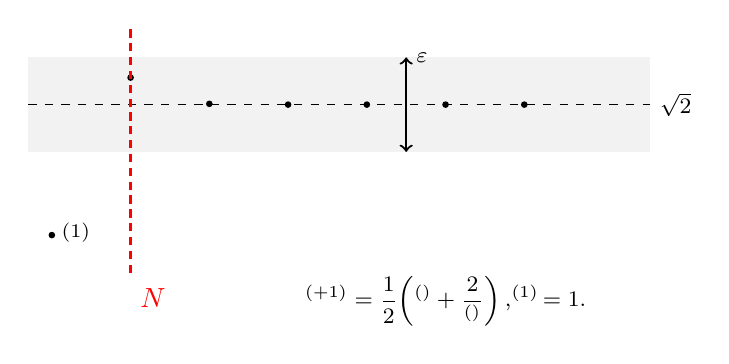
\begin{tikzpicture}[x=1cm,y=4cm]
        \def\srtwo{1.4142}
        \def\eps{0.15}
        \def\nmax{7}
        \fill[gray!30, opacity=0.35] (-0.3,{\srtwo-\eps}) rectangle (\nmax+0.6,{\srtwo+\eps});
        \draw[<->, thick] (4.5,{\srtwo-\eps}) -- (4.5,{\srtwo+\eps}) node[above, right] {\footnotesize{$\varepsilon$}};
        \draw[dashed] (-0.3,\srtwo) -- (\nmax+0.6,\srtwo) node[right] {\footnotesize{$\sqrt{2}$}};
        \fill (0,1.0000) circle (1.2pt) node [right] {$\feature^{(1)}$};
        \fill (1,1.5000) circle (1.2pt);
        \fill (2,1.4167) circle (1.2pt);
        \fill (3,1.4142) circle (1.2pt);
        \fill (4,1.41421) circle (1.2pt);
        \fill (5,1.4142136) circle (1.2pt);
        \fill (6,1.41421356) circle (1.2pt);
        \def\N{1}
        \draw[densely dashed, thick, red] (\N,0.88) -- (\N,1.655);
        \node[right, red] at (\N,0.8) {$N$};
        \node[align=right, anchor=north, font=\small] at (5,0.9) 
        {\footnotesize{$\displaystyle \feature^{(\sampleidx+1)}=\frac{1}{2}\!\left(\feature^{(\sampleidx)}+\frac{2}{\feature^{(\sampleidx)}}\right), \feature^{(1)}=1.$}};
    \end{tikzpicture}
    \caption{Eine Cauchy-\gls{sequence} 
    $\big(\feature^{(\sampleidx)}\big)_{\sampleidx\in\mathbb{N}}$ 
    im \gls{metricspace} $\pair{\mathbb{Q}}{|\cdot|}$. 
    Diese \gls{sequence} wird durch ein \gls{fixedpointiter} erzeugt, um $\sqrt{2}$ zu approximieren. 
    Für alle $\sampleidx \ge N$ liegen die Folgenglieder innerhalb eines Bandes der Breite $\varepsilon$. 
    Beachte, dass die \gls{sequence} in $\mathbb{Q}$ nicht konvergiert, da $\sqrt{2} \notin \mathbb{Q}$ \cite[Beispiel 1.1]{RudinBookPrinciplesMatheAnalysis}.\label{fig:fpit_cauchy_sqrt2_dict}}
    \end{figure}
    Abb.\ \ref{fig:fpit_cauchy_sqrt2_dict} zeigt eine Cauchy-Folge im \gls{metricspace} $\pair{\mathbb{Q}}{|\cdot|}$ der rationalen Zahlen. \\
    Siehe auch: \gls{metricspace}, \gls{sequence}.},
    type=math,
    first={Cauchy-Folge},
    text={Cauchy-Folge},
    plural={Cauchy-Folgen},
    firstplural={Cauchy-Folgen}
}

\newglossaryentry{nonexpansiveop}{
    name={nicht-expansiver Operator},
    description={Ein \index{nicht-expansiver Operator} Operator 
    $\fixedpointop: \hilbertspace \rightarrow \hilbertspace$, definiert auf einem 
    \gls{hilbertspace} $\hilbertspace$, heißt nicht-expansiv, wenn er die Abstände 
    nicht vergrößert. Anders ausgedrückt gilt:
    \[
    \normgeneric{ \fixedpointop \weights - \fixedpointop \weights'}{2} 
    \leq \normgeneric{\weights - \weights'}{2} \quad \text{für alle } \weights, \weights' \in \hilbertspace.
    \]
    Siehe auch: \gls{fixedpointiter}, \gls{contractop}.},
    type=math,
    first={nicht-expansiver Operator},
    text={nicht-expansiver Operator},
    plural={nicht-expansive Operatoren},
    firstplural={nicht-expansive Operatoren}
}


\newglossaryentry{fixedpointiter}
{name={fixed-point iteration},
	description={A\index{fixed-point iteration} fixed-point iteration is an iterative method for solving 
		a given \gls{optproblem}. It constructs a sequence $\weights^{(0)}, \weights^{(1)}, \ldots$ by 
		 repeatedly applying an operator $\fixedpointop$, i.e., 
		 \begin{equation} 
		 	\label{equ_def_fixed_point_dict} 
		 	\weights^{(\iteridx+1)} = \fixedpointop \weights^{(\iteridx)} \mbox{, for } \iteridx=0, 1, \ldots.
		 \end{equation} 
		 The operator $\fixedpointop$ is chosen such that any of its fixed points is a solution 
		 $\widehat{\weights}$ to the given \gls{optproblem}. For example, given a \gls{differentiable} and 
		 \gls{convex} \gls{function} $f(\weights)$, the fixed points of the operator $\fixedpointop: \weights \mapsto \weights - \nabla f(\weights)$ 
		 coincide with the minimizers of $f(\weights)$. In general, for a given \gls{optproblem} with solution $\widehat{\weights}$, 
		 there are many different operators $\fixedpointop$ whose fixed points are $\widehat{\weights}$. 
		 Clearly, we should use an operator $\fixedpointop$ in \eqref{equ_def_fixed_point_dict} that reduces the distance to a solution such that
		 \begin{equation} 
			\nonumber
			\underbrace{\normgeneric{ \weights^{(\iteridx+1)} - \widehat{\netparams}}{2}}_{\stackrel{\eqref{equ_def_fixed_point_dict}}{=} \normgeneric{ \fixedpointop \weights^{(\iteridx)} - \fixedpointop\widehat{\weights}}{2}}  \leq 	\normgeneric{ \weights^{(\iteridx)} - \widehat{\weights}}{2}. 
		\end{equation}
		Thus, we require $\fixedpointop$ to be at least non-expansive, i.e., the iteration \eqref{equ_def_fixed_point_dict} 
		should not result in worse \glspl{modelparam} that have a larger distance to a solution $\widehat{\weights}$. 
		Furthermore, each iteration \eqref{equ_def_fixed_point_dict} should also make some progress, i.e., 
		reduce the distance to a solution $\widehat{\weights}$. This requirement can be made precise using 
		the notion of a \gls{contractop} \cite{Bauschke:2017}, \cite{fixedpoinIsta}. 
		The operator $\fixedpointop$ is a \gls{contractop} if, for some $\contractfac \in [0,1)$,
		\begin{equation} 
			\nonumber
			\normgeneric{ \fixedpointop \weights\!-\!\fixedpointop \weights'}{2}  \leq  \contractfac	\normgeneric{\weights\!-\!\weights'}{2} \mbox{ holds for any } \weights,\weights'.
		\end{equation}
		For a \gls{contractop} $\fixedpointop$, the fixed-point iteration \eqref{equ_def_fixed_point_dict} generates 
		a sequence $\weights^{(\iteridx)}$ that converges quite rapidly. In particular \cite[Th. 9.23]{RudinBookPrinciplesMatheAnalysis}, 
		\begin{equation} 
			\nonumber
			\normgeneric{ \weights^{(\iteridx)} - \widehat{\weights}}{2} \leq \contractfac^{\iteridx} 	\normgeneric{ \weights^{(0)} - \widehat{\weights}}{2}. 
		\end{equation} 
		Here, $\normgeneric{ \weights^{(0)} - \widehat{\weights}}{2}$ is the distance between 
		the initialization $\weights^{(0)}$ and the solution $\widehat{\weights}$. 
		It turns out that a fixed-point iteration \eqref{equ_def_fixed_point_dict} with a firmly non-expansive 
		operator $\fixedpointop$ is guaranteed to converge to a fixed-point of $\fixedpointop$ \cite[Cor. 5.16]{Bauschke:2017}. 
		Fig. \ref{fig_examples_nonexp_dict} depicts examples of a firmly non-expansive operator, a non-expansive operator, 
		and a \gls{contractop}. All these operators are defined on the one-dimensional space $\mathbb{R}$. 
		Another example of a firmly non-expansive operator is the \gls{proxop} of a \gls{convex} \gls{function} \cite{Bauschke:2017}, \cite{ProximalMethods}. 
		\definecolor{darkgreen}{rgb}{0.0, 0.5, 0.0}
		\begin{figure}[H]
			\begin{center} 
				\begin{tikzpicture}[scale=1.5]
					% Axes
					\draw[line width=1pt, ->] (-2,0) -- (2,0) node[right] {$\weight^{(\iteridx)}$};
					\draw[line width=1pt, ->] (0,-2) -- (0,2) node[above] {$\weight^{(\iteridx+1)}$};
					% Labels
					\node at (2.1,2.2) {$\fixedpointop^{(3)}$};
					\node at (1.9,-1.5) {$\fixedpointop^{(1)}$};
					\node at (1.5,1.2) {$\fixedpointop^{(2)}$};
					% Dashed lines at x=1 and y=1
					\draw[dashed] (1,-2) -- (1,2); % Vertical line at x=1
					\draw[dashed] (-2,1) -- (2,1); % Horizontal line at y=1
					\draw[dashed] (-2,-1) -- (2,-1); % Horizontal line at y=1
					\draw[dashed] (-1,-2) -- (-1,2); % Vertical line at x=1
					\node[above,xshift=4pt,yshift=-1pt] at (1,0) {$1$};
					\node[above,xshift=8pt,yshift=-1pt] at (0,-1) {$-1$};
					% First curve: y = 1/2 x + 1
					\draw[line width=2,domain=-2:2,smooth,blue] plot(\x,{0.5*\x + 1});
					% Second curve: y = -x
					\draw[line width=2,domain=-2:2,smooth,red] plot(\x,{-\x});
					% Third curve: y = x / |x| * min(|x|, 1)
					\draw[line width=2, domain=-2:-1,smooth,darkgreen] plot(\x,{-1});
					\draw[line width=2,domain=-1:1,smooth,darkgreen] plot(\x,{\x});
					\draw[line width=2,domain=1:2,smooth,darkgreen] plot(\x,{1});
				\end{tikzpicture}
			\end{center} 
			\caption{Example of a non-expansive operator $\fixedpointop^{(1)}$, a firmly non-expansive operator $\fixedpointop^{(2)}$, and 
				a \gls{contractop} $\fixedpointop^{(3)}$. \label{fig_examples_nonexp_dict}}
		\end{figure} 
		See also: \gls{optproblem}, \gls{differentiable}, \gls{convex} \gls{function}, \glspl{modelparam}, \gls{contractop}, \gls{proxop}.},
	first={fixed-point iteration},
	text={fixed-point iteration},
	firstplural={fixed-point iterations}, 
	plural={fixed-point iterations}
}


\newglossaryentry{ergraph}
{name={Erd\H{o}s-R\'enyi graph (ER graph)},
	description={An ER  \gls{graph} is a \gls{probmodel} for \glspl{graph} defined over 
		a given node set $\nodeidx=1, \ldots, \nrnodes$. One way to define the ER \gls{graph} is 
		via the collection of \gls{iid} binary \glspl{rv} $b^{(\edge{\nodeidx}{\nodeidx'})} \in \{0,1\}$, 
		for each pair of different nodes $\nodeidx, \nodeidx'$. A specific \gls{realization}  
		of an ER \gls{graph} contains an edge $\edge{\nodeidx}{\nodeidx'}$ if and only if 
		$b^{(\edge{\nodeidx}{\nodeidx'})}=1$. The ER \gls{graph} is parameterized by the 
		number $\nrnodes$ of nodes and the \gls{probability} $\prob{b^{(\edge{\nodeidx}{\nodeidx'})}=1}$. 
		\\
		See also: \gls{graph}, \gls{probmodel}, \gls{iid}, \gls{rv}, \gls{realization}, \gls{probability}.},
	first={Erd\H{o}s-R\'enyi (ER) graph},
	text={ER graph}
}

\newglossaryentry{attack}
{name={attack},  
	description={An attack\index{attack} on an \gls{ml} system refers to an intentional action—either 
		active or passive—that compromises the system's integrity, availability, or confidentiality. 
		Active attacks involve perturbing components such as \glspl{dataset} (via \gls{datapoisoning}) 
		or communication links between \glspl{device} within an \gls{ml} application. Passive attacks, 
		such as \glspl{privattack}, aim to infer \glspl{sensattr} without modifying the system. 
		Depending on their goal, we distinguish between \glspl{dosattack}, \gls{backdoor} attacks, and \glspl{privattack}.
		\\
		See also: \gls{datapoisoning}, \gls{privattack}, \gls{sensattr}, \gls{dosattack}, \gls{backdoor}.},
	plural={attacks}, 
	first={attack},
	firstplural={attacks},
	text={attack}
}

\newglossaryentry{privattack}
{name={privacy attack},
	description={A privacy \gls{attack}\index{privacy attack} on an \gls{ml} system aims to infer 
		\glspl{sensattr} of individuals by exploiting partial access to a trained \gls{ml} \gls{model}. 
		One form of a privacy \gls{attack} is \gls{modelinversion}.\\
		See also: \gls{attack}, \gls{sensattr}, \gls{modelinversion}, \gls{trustAI}, \gls{gdpr}.},
	plural={privacy attacks}, 
	first={privacy attack},
	firstplural={privacy attacks}, 
	text={privacy attack}
}



\newglossaryentry{epigraph}
{name={Epigraphh},
  description={Der Epigraph \index{epigraph} einer reelwertigen Funktion $f : \mathbb{R}^n \to \mathbb{R} \cup \{+\infty\}$ 
  	is die Menge aller Punkte, die auf oder über diesem Graph liegen:
		\[
		\operatorname{epi}(f) = \left\{ (\mathbf{x}, t) \in \mathbb{R}^n \times \mathbb{R} \,\middle|\, f(\mathbf{x}) \leq t \right\}.
		\]
		Eine Funktion ist \gls{convex} genau dann, wenn ihr Epigraph eine \gls{convex}e Menge is \cite{BoydConvexBook,BertCvxAnalOpt}.
		\begin{figure}[H]
			\centering
			\begin{tikzpicture}[scale=1.0]
				\begin{axis}[
					axis lines = middle,
					xlabel = $x$,
					ylabel = {},
					xmin=-2, xmax=2,
					ymin=0, ymax=4.5,
					samples=100,
					domain=-1.5:1.5,
					thick,
					width=8cm,
					height=6cm,
					grid=none,
					axis on top,
					]
					% Function
					\addplot [blue, thick, domain=-1.5:1.5] {x^2} node [pos=0.85, anchor=south west, xshift=5pt] {$f(x)$};
					% Epigraph shading
					\addplot [
					name path=f,
					draw=none,
					ytick=\empty,
					domain=-1.5:1.5,
					] {x^2};
					\path[name path=top] (axis cs:-1.5,4) -- (axis cs:1.5,4);
					\addplot [
					blue!20,
					opacity=0.6,
					draw=none,
					] fill between [
					of=f and top,
					soft clip={domain=-1.5:1.5},
					];
					    \node[font=\small] at (axis cs:-1.0,2.3) {$\operatorname{epi} f$};
				%	\node[align=center, fill=white, draw=black, rounded corners, font=\small] at (axis cs:0.5,3.5) {Epigraph\\$\{(x,t) \mid f(x) \le t\}$};
				\end{axis}
			\end{tikzpicture}
			\caption{Epigraph of the function $f(x) = x^2$ (shaded area).}
		\end{figure}
	},
	first={Epigraph},
	text={Epigraph},
	plural={Epigraphen}
}

\newglossaryentry{nullspace}{
    name={Nullraum},
    description={Der \index{Nullraum} Nullraum einer \gls{matrix} 
    $\mA \in \mathbb{R}^{\nrfeatures' \times \nrfeatures}$, bezeichnet als 
    $\nullspace{\mA}$, ist die Menge aller \glspl{vector} 
    $\mathbf{n} \in \mathbb{R}^\nrfeatures$, für die gilt:
    \[
    \mA \mathbf{n} = \mathbf{0}.
    \]
    Betrachten wir eine \gls{featlearn}-Methode, die die \gls{matrix} $\mA$ verwendet, um einen 
    \gls{featurevec} $\mathbf{x} \in \mathbb{R}^{\nrfeatures}$ eines \gls{datapoint} in einen neuen 
    \gls{featurevec} $\vz = \mA \mathbf{x} \in \mathbb{R}^{\nrfeatures'}$ zu transformieren. 
    Der Nullraum $\nullspace{\mA}$ beschreibt alle Richtungen im ursprünglichen 
    \gls{featurespace} $\mathbb{R}^{\nrfeatures}$, entlang derer die Transformation 
    $\mA \mathbf{x}$ unverändert bleibt. Anders gesagt: Das Hinzufügen eines beliebigen \gls{vector} 
    aus dem Nullraum zu einem \gls{featurevec} $\featurevec$ verändert die transformierte 
    Repräsentation $\vz$ nicht. Diese Eigenschaft kann genutzt werden, um Invarianzen in den 
    \glspl{prediction} (berechnet aus $\mA \mathbf{x}$) zu erzwingen. 
    Fig.\ \ref{fig:nullspace-rotation-dict} illustriert eine solche Invarianz. 
    Es werden rotierte Versionen zweier handgeschriebener Ziffern gezeigt, die sich annähernd auf 1D-Kurven im 
    ursprünglichen \gls{featurespace} befinden. Diese Kurven sind entlang einer Richtungs-\gls{vector} 
    $\mathbf{n} \in \mathbb{R}^{\nrfeatures}$ ausgerichtet. Um sicherzustellen, dass das trainierte \gls{model} 
    gegenüber solchen Rotationen invariant ist, kann die Transformations-\gls{matrix} $\mA$ so gewählt werden, 
    dass $\mathbf{n} \in \nullspace{\mA}$. Dadurch bleibt $\mA \mathbf{x}$ und damit die resultierende 
    \gls{prediction} ungefähr unverändert bei Rotation des Eingabebildes.
    \begin{figure}[H]
        \centering
        \includegraphics[width=0.6\textwidth]{assets/pythonsnacks/nullspace_0_1.png}
        \caption{
        Rotierte Handschriften zweier verschiedener Ziffern. Die Rotationen liegen annähernd 
        entlang von Geraden, die parallel zum \gls{vector} $\mathbf{n}$ verlaufen. Für einen 
        binären \gls{classifier}, der diese Ziffern unterscheidet, ist eine natürliche Wahl 
        eine lineare \gls{featuremap} $\featurevec \mapsto \mathbf{A}\featurevec$ mit einer 
        \gls{matrix} $\mA$, deren Nullraum $\mathbf{n}$ enthält, d.h. $\mathbf{n} \in \mathrm{null}(\mA)$.
        \label{fig:nullspace-rotation-dict}}
    \end{figure}
    Siehe auch: \gls{matrix}, \gls{featuremap}, \gls{featlearn}. \\
    Python-Demo: \href{https://github.com/AaltoDictionaryofML/AaltoDictionaryofML.github.io/blob/main/assets/pythonsnacks/nullspace.py}{klicke hier}},
    first={Nullraum},
    firstplural={Nullräume},
    plural={Nullräume},
    text={Nullraum}
}

\newglossaryentry{maximum}
{name=Maximum,
 %description={Given a set of real numbers, the maximum\index{maximum} is the largest of those numbers.},
     description={Das Maximum \index{maximum} einer Menge $\mathcal{A} \subseteq \mathbb{R}$ 
     	von reellen Zahlen ist das größte Element dieser Menge, dalls ein solches Element existiert. Eine Menge $\mathcal{A}$ 
     	besitzt ein Maximum, wenn sie nach oben beschränkt ist und ihr \gls{supremum} erreicht. \cite[Sec.~1.4]{RudinBookPrinciplesMatheAnalysis}.},
 first={Maximum},text={Maximum}, plural={Maxima}
}

\newglossaryentry{supremum}
{name=Supremum (oder kleinste obere Schranke),
	description={Das Supremum \index{supremum (oder die kleinste obere Schranke} einer Menge reeller Zahlen ist die kleinste Zahl, die größer oder gleich jedem Element der Menge ist.
	Genauer gesagt, eine reelle Zahl $a$ ist das Supremum einer Menge $\mathcal{A} \subseteq \mathbb{R}$, wenn folgende Bedingungen erfüllt sind 1) $a$ ist eine obere Schranke von $\mathcal{A}$; und 
	 2) es gibt keine Zahl die kleiner ist als $a$ und gleichzeiting ebenfalls eine obere Schranke von $\mathcal{A}$ ist. Jede nichtleere, nach oben beschränkte Menge reeller Zahlen besitzt ein Supremum, 
	 selbst dann wenn das Supremum nicht zur Menge gehört \cite[Sec.~1.4]{RudinBookPrinciplesMatheAnalysis}.},
	first={Supremum (oder kleinste obere Schranke)},text={Supremum}, plural= {Suprema}
	
    Formaler ausgedrückt ist eine reelle Zahl $a$ das Supremum einer Menge 
$\mathcal{A} \subseteq \mathbb{R}$, wenn gilt: 1) $a$ ist eine obere Schranke von $\mathcal{A}$; 
und 2) keine Zahl, die kleiner als $a$ ist, ist eine obere Schranke von $\mathcal{A}$. 
Jede nichtleere, nach oben beschränkte Menge reeller Zahlen besitzt ein Supremum, 
selbst wenn dieses Supremum nicht als Element in der Menge enthalten ist 
\cite[Abschnitt~1.4]{RudinBookPrinciplesMatheAnalysis}.
},
first={Supremum (oder kleinste obere Schranke)},
text={Supremum}
}
%potenzielle Quelle fuer Maximum und Supremum, onlinelexikon uni stuttgart : https://mo.mathematik.uni-stuttgart.de/inhalt/aussage/aussage376/
%tbc

\newglossaryentry{discrepancy}
{name=Diskrepanz,
	description={
		Consider\index{discrepancy} an \gls{fl} application with \gls{netdata} 
		represented by an \gls{empgraph}. \gls{fl} methods use a discrepancy measure 
		to compare \gls{hypothesis} maps from \gls{localmodel}s at nodes $\nodeidx,\nodeidx'$ 
		connected by an edge in the \gls{empgraph}.},
	first={discrepancy},text={discrepancy}
}

\newglossaryentry{FedRelax}
{name={FedRelax},
	description={An\index{FedRelax} \gls{fl} \gls{distributedalgorithm}. 
		\\ 
		See also: \gls{fl}, \gls{algorithm}.},
	first={FedRelax},text={FedRelax}
} 

\newglossaryentry{fedavg}{
    name={federated averaging (FedAvg)},
    description={FedAvg\index{federated averaging (FedAvg)} bezeichnet eine Familie iterativer \gls{fl}-\glspl{algorithm}. 
    Dabei wird ein Server-Client-Setting verwendet, das zwischen clientseitigem \gls{localmodel}-Training und der 
    Aggregation der aktualisierten \glspl{modelparam} auf dem Server wechselt \cite{pmlr-v54-mcmahan17a}. 
    Das lokale Update beim Client $\nodeidx=1, \ldots, \nrnodes$ zum Zeitpunkt $\iteridx$ startet von den aktuellen 
    \glspl{modelparam} $\weights^{(\iteridx)}$, die vom Server bereitgestellt werden, und besteht typischerweise darin, 
    wenige Iterationen von \gls{stochGD} auszuführen. Nach Abschluss der lokalen Updates aggregiert der Server die 
    Ergebnisse (z.\,B. durch Mittelung). 
    Fig.\ \ref{fig_single_iteration_fedavg_dict} zeigt die Ausführung einer einzelnen Iteration von FedAvg.
    \begin{figure}[H]
        \begin{center}
        \begin{tikzpicture}[>=Stealth, node distance=1cm and 1.5cm, every node/.style={font=\small}]
        % Styles
        \tikzstyle{server} = [circle, fill=black, minimum size=6pt, inner sep=0pt]
        \tikzstyle{client} = [circle, draw=black, minimum size=6pt, inner sep=0pt]
        % Time step labels
        \node (label1) at (0,3.5) {Broadcast};
        \node[right=2.5cm of label1] (label2) {Lokales Update};
        \node[right=2.5cm of label2] (label3) {Aggregation};
        % Time step k
        \node[server] (s1) at (label1 |- 0,2.5) {};
        \node[client] (c1l) at ($(s1) + (-1cm,-1cm)$) {};
        \node[client] (c1r) at ($(s1) + (1cm,-1cm)$) {};
        \node[] (dots1) at ($(s1) + (0cm,-1cm)$) {\ldots};
        \draw[->] (s1) -- (c1l) node[midway,left] {$\weights^{(\iteridx)}$};
        \draw[->] (s1) -- (c1r) node[midway,right] {$\weights^{(\iteridx)}$};
        \draw[->] (s1) -- (dots1);
        % Time step k+1 (local updates)
        \node[server] (s2) at (label2 |- 0,2.5) {};
        \node[client] (c2l) at ($(s2) + (-1cm,-1cm)$) {};
        \node[client] (c2r) at ($(s2) + (1cm,-1cm)$) {};
        \node[] (dots2) at ($(s2) + (0cm,-1cm)$) {\ldots};
        \node[below=0.2cm of c2l] {$\localparamsiter{\iteridx}{1}$};
        \node[below=0.2cm of c2r] {$\localparamsiter{\iteridx}{\nrnodes}$};
        % Time step k+2 (aggregation)
        \node[server] (s3) at (label3 |- 0,2.5) {};
        \node[above=0.01cm of s3, yshift=-4pt] {$\weights^{(\iteridx+1)}$};
        \node[client] (c3l) at ($(s3) + (-1cm,-1cm)$) {};
        \node[client] (c3r) at ($(s3) + (1cm,-1cm)$) {};
        \node[] (dots3) at ($(s3) + (0cm,-1cm)$) {\ldots};
        \draw[->] (c3l) -- (s3) node[midway,left] {$\localparamsiter{\iteridx}{1}$};
        \draw[->] (c3r) -- (s3)  node[midway,right] {$\localparamsiter{\iteridx}{\nrnodes}$};
        \draw[->] (dots3) -- (s3);
        \end{tikzpicture}
        \end{center}
        \caption{Illustration einer einzelnen Iteration von FedAvg: Der Server sendet \glspl{modelparam} an die Clients, 
        diese führen lokale Updates durch, und der Server aggregiert anschließend die aktualisierten Parameter. 
        \label{fig_single_iteration_fedavg_dict}} 
    \end{figure} 
    Siehe auch: \gls{fl}, \gls{algorithm}, \gls{localmodel}, \gls{stochGD}.},
    first={FedAvg},
    text={FedAvg}
}


\newglossaryentry{FedGD}
{name={FedGD},
	description={An\index{FedGD} \gls{fl} \gls{distributedalgorithm} that 
		can be implemented as message passing across an \gls{empgraph}. 
		\\ 
		See also: \gls{fl}, \gls{algorithm}, \gls{gradstep}, \gls{gdmethods}.},
	first={FedGD},text={FedGD}
} 

\newglossaryentry{FedSGD}
{name={FedSGD},
	description={An\index{FedSGD} \gls{fl} \gls{distributedalgorithm} that 
		can be implemented as message passing across an \gls{empgraph}. 
		\\ 
		See also: \gls{fl}, \gls{algorithm}, \gls{gradstep}, \gls{gdmethods}, \gls{stochGD}.},
	first={FedSGD},text={FedSGD}

\newglossaryentry{hfl}
{name={horizontales kollaboratives Lernen (HFL)},description=
	{HFL\index{horizontal federated learning (HFL)} nutzt \glspl{localdataset} die aus verschiedenen
		\gls{datapoint}en, jedoch mit denselben \gls{feature}en beschrieben werden \cite{HFLChapter2020}.
	Ein Beispiel dafür ist die Wettervorhersage mit einem Netzwerk räumlich verteilter 
	Wetterbeobachtungsstationen. Jede Wetterstation misst dieselben Größen, 
	z. B. tägliche Temperatur, Luftdruck und Niederschlag.
		Allerdings erfassen die verschiedenen Stationen die Merkmale unterschiedlicher 
	raum-zeitlicher Regionen.
	Jede dieser Regionen stellt einen individuellen  \gls{datapoint}  dar, 
	der durch dieselben \glspl{feature}  (z.B. tägliche Temperatur oder Luftdruck) charakterisiert werden. \\
	Siehe auch: \gls{fl}, \gls{vfl}, \gls{cfl}. },
	first={HFL},text={HFL}
}

\newglossaryentry{dimred}
{name={Dimensionalitätsreduktion},
	description= Dimensionalitätsreduktion \index{dimensionality reduction} bezeichnet Methoden, die 
	(typischerweise viele) rohe  \glspl{feature} auf eine (relativ kleiner Menge)  neuer  \glspl{feature} abbilden.
	Diese Methoden können genutzt werden um \glspl{datapoint} zu visualisieren, indem zwei  \glspl{feature}
	gelernt weden, die als Koordinaten für die Darstellung in einem \gls{scatterplot} dienen. },
	 first={Dimensionalitätsreduktion},text={Dimensionalitätsreduktion}, plural={Dimensionalitätsreduktionen}
} 

\newglossaryentry{diagnosis}{
    name={Diagnose},
    description={Betrachten wir eine \gls{erm}-basierte Methode, die zu einem trainierten \gls{model} 
    (oder gelernten \gls{hypothesis}) $\learnthypothesis \in \hypospace$ geführt hat. 
    Wir können die Methode diagnostizieren, indem wir den \gls{trainerr} $\trainerror$ 
    mit dem \gls{valerr} $\valerror$ vergleichen, der von $\learnthypothesis$ auf dem 
    \gls{trainset} bzw. \gls{valset} erzielt wird.
    \begin{figure}[htbp]
    \begin{center}
        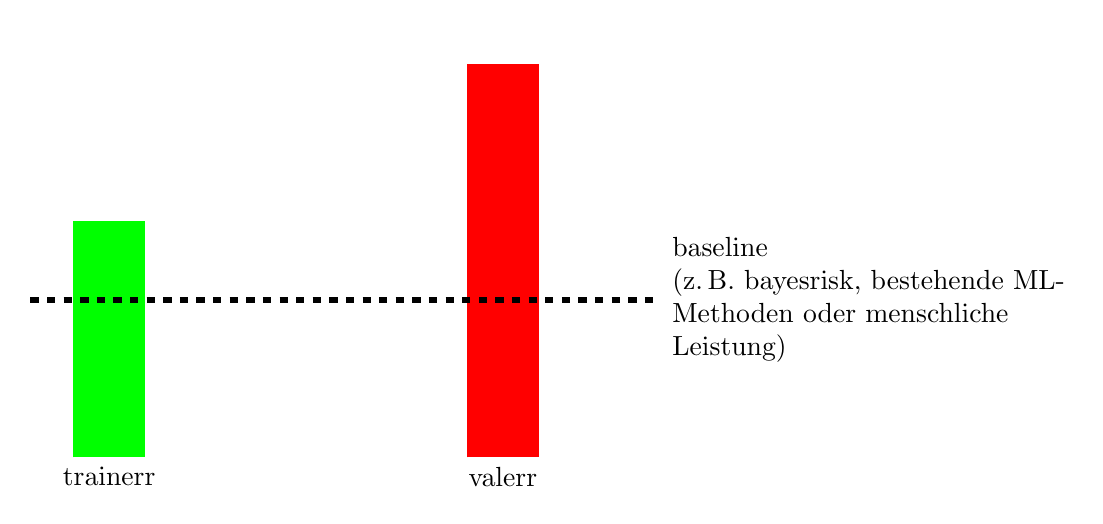
\begin{tikzpicture}[ycomb]
            \draw[color=green,line width=26pt]
            plot coordinates{(0,3)};
            \node [below] at (0,0) {\gls{trainerr}} ; 
            \draw[color=red,line width=26pt]
            plot coordinates{(5,5)};
            \node [below] at (5,0) {\gls{valerr}} ; 
            \draw[dashed,line width=2] (-1,2) -- (7,2) node[right,text width=5cm]{\gls{baseline} \\ (z.\,B. \gls{bayesrisk}, bestehende ML-Methoden oder menschliche Leistung)};
        \end{tikzpicture}
    \end{center}
    \caption{Diagnose einer \gls{erm}-basierten Methode durch Vergleich von \gls{trainerr} und \gls{valerr}. 
    Idealerweise liegen beide Werte auf dem Niveau der \gls{baseline}.\label{fig_diagnosis_dict}}
    \end{figure}
    Siehe auch: \gls{validation}, \gls{kfoldcv}, \gls{generalization}, \gls{baseline}.},
    first={Diagnose},
    text={Diagnose},
	plural={Diagnosen}
}



\newglossaryentry{ml}
{name={Maschinelles Lernen (ML)},
	description={ML\index{machine learning (ML)} zielt darauf ab, ein  \gls{label} anhand der \glspl{feature} eines
		\gls{datapoint} es vorherzusagen. 
		ML-Methoden erreichen dies, indem sie eine \gls{hypothesis aus einem \gls{hypospace} (oder  \gls{model})
			durch Minimierung einer \gls{lossfunc}\cite{MLBasics},  \cite{HastieWainwrightBook} erlernen.
			Eine präzise Formulierung dieses Prinzips ist die \gls{erm}.Verschieden ML-Methoden ergeben sich aus verschiedenen 
			Designentscheidungen für \glspl{datapoint}  {d.h. deren \glspl{features und \glspl{label} }, 
				das \gls{model} und die \gls{lossfunc} \cite[Ch. 3]{MLBasics}.},
	first={Maschinelles Lernen (ML)},text={ML}
} 


\newglossaryentry{reinforcementlearning}
{name={reinforcement learning (RL)},
	description={
	RL\index{reinforcement learning (RL)} refers to a \gls{onlinelearning} setting where 
	we can only evaluate the usefulness of a single \gls{hypothesis} (i.e., a choice of \gls{model} \glspl{parameter}) 
	at each time step $\timeidx$. In particular, RL methods apply the current \gls{hypothesis} 
	$\hypothesis^{(\timeidx)}$ to the \gls{featurevec} $\featurevec^{(\timeidx)}$ of the 
	newly received \gls{datapoint}. The usefulness of the resulting \gls{prediction} 
	$\hypothesis^{(\timeidx)}(\featurevec^{(\timeidx)})$ is quantified by a \gls{reward} 
	signal $\reward^{(\timeidx)}$. 
	\begin{figure}
			\begin{center}
		\begin{tikzpicture}[scale=1]
			\draw[->] (-2, 0) -- (6, 0);
			\node at (6.3, 0) {$\hypothesis$};
	        % loss at time t 
			\draw[thick, blue, domain=0:3, samples=20] plot (\x-3, {-0.2*(\x)^2 + 2});
			\node[anchor=west,yshift=4pt] at (0-3, {-0.2*(0)^2 + 2}) {$-\loss^{(\timeidx)}(\hypothesis)$};
			% Marker and hypothesis label for h^(t)
			\filldraw[blue] (1.5-3, {-0.2*(1.5)^2 + 2}) circle (2pt);
			\node[anchor=north] at (1.5-3, -0.3) {$\hypothesis^{(\timeidx)}$};		
			\draw[dotted] (1.5-3, 0) -- (1.5-3, {-0.2*(1.5)^2 + 2});
			%%% time t+1
			\draw[thick, red, domain=0:5, samples=20, dashed] plot (\x, {-0.15*(\x - 2)^2 + 3});
			\node[anchor=west,yshift=4pt] at (3, {-0.15*(3 - 2)^2 + 3}) {$-\loss^{(\timeidx+1)}(\hypothesis)$};
			\filldraw[red] (2, {-0.15*(2 - 2)^2 + 3}) circle (2pt);
			\node[anchor=north] at (2, -0.3) {$\hypothesis^{(\timeidx+1)}$};
			\draw[dotted] (2, 0) -- (2, {-0.15*(3 - 2)^2 + 3});
			%%% time t+2
			\draw[thick, green!60!black, domain=3:5, samples=20, dotted] plot (\x+2, {-0.1*(\x - 4)^2 + 1.5});
			\node[anchor=west,yshift=4pt] at (4.5+2, {-0.1*(4.5 - 4)^2 + 1.5}) {$-\loss^{(\timeidx+2)}(\hypothesis)$};
			\filldraw[green!60!black] (3.5+2, {-0.1*(3.5 - 4)^2 + 1.5}) circle (2pt);
			\node[anchor=north] at (3.5+2, -0.3) {$\hypothesis^{(\timeidx+2)}$};
			\draw[dotted] (3.5+2, 0) -- (3.5+2, {-0.1*(3.5 - 4)^2 + 1.5});
		\end{tikzpicture}
		\caption{Three consecutive time steps $\timeidx,\timeidx+1,\timeidx+2$ with corresponding \glspl{lossfunc} $\loss^{(\timeidx)},
		\loss^{(\timeidx+1)}, \loss^{(\timeidx+2)}$. During time step $\timeidx$, a RL method can evaluate the 
		\gls{lossfunc} only for one specific \gls{hypothesis} $\hypothesis^{(\timeidx)}$, resulting in the \gls{reward} 
		signal $\reward^{(\timeidx)}=-\loss^{(\timeidx)}(\hypothesis^{(\timeidx)})$.}
			\end{center}
	\end{figure}
	In general, the \gls{reward} depends also on the 
	previous \glspl{prediction} $\hypothesis^{(\timeidx')}\big(\featurevec^{(\timeidx')}\big)$ 
	for $\timeidx' < \timeidx$. The goal of RL is to learn $\hypothesis^{(\timeidx)}$, for 
	each time step $\timeidx$, such that the (possibly discounted) cumulative \gls{reward} 
	is maximized \cite{MLBasics}, \cite{SuttonEd2}.
		\\
		See also: \gls{lossfunc}, \gls{reward}, \gls{ml}.},
	first={reinforcement learning (RL)},
	text={RL}
}

\newglossaryentry{featlearn}
{name={Merkmalslernen},
	description={Betrachten wir eine  \gls{ml} Anwendung mit  \glspl{datapoint} die durch rohe  \glspl{feature} $\featurevec \in \featurespace$ beschrieben 
		werden. \Gls{feature}lernen \index{feature learning} (auch: Feature learning)  bezeichnet die Aufgabe, eine Abbildung
		$$\featuremapvec: \featurespace \rightarrow \featurespace': \featurevec \mapsto \featurevec'$$ 
		zu lernen, welche rohe \glspl{feature} $\featurevec \in \featurespace$ eines \gls{datapoint}es einliest 
		und neue \glspl{feature} $\featurevec' \in \featurespace'$ aus einem neuen \gls{featurespace} 
		$\featurespace'$ erzeugt. Verschiedene Methoden des \gls{feature}slernens ergeben sich aus unterschiedlichen 
		Gestaltungsentscheidungen für $\featurespace,\featurespace'$,  einem \gls{hypospace} $\hypospace$ möglicher Abbildungen $\featuremapvec$
		sowie einem quantitativen Maß für die Nützlichkeit einer bestimmten Abbildung  $\featuremapvec \in \hypospace$.
		Ein Beispiel ist \gls{pca}, wobei gilt: 
		$\featurespace \defeq \mathbb{R}^{\dimlocalmodel}$, $\featurespace' \defeq \mathbb{R}^{\dimlocalmodel'}$ 
		mit $\dimlocalmodel' < \dimlocalmodel$, und ein \gls{hypospace}
		$$\hypospace\defeq \big\{ \featuremapvec: \mathbb{R}^{\dimlocalmodel}
		\!\rightarrow\! \mathbb{R}^{\dimlocalmodel'}\!:\!\featurevec'\!\defeq\!\mF \featurevec \mbox{ mit } \mF \!\in\! \mathbb{R}^{\dimlocalmodel' \times \dimlocalmodel} \big\}.$$
		\Gls{pca} bewertet die Nützlichkeit einer bestimmten Abbildung $\featuremapvec(\featurevec)= \mF \featurevec$ 
		durch den \gls{minimalen} linearen Rekonstruktionsfehler auf einem \gls{dataset}, also
		$$\min_{\mG \in \mathbb{R}^{\dimlocalmodel \!\!\!\times \dimlocalmodel'}} \sum_{\sampleidx=1}^{\samplesize} \normgeneric{\mG \mF \featurevec^{(\sampleidx)} - \featurevec^{(\sampleidx)}}{2}^{2}.$$ 
			\\ 
	
	first={Merkmalslernen},text={Merkmalslernen}
} 

\newglossaryentry{autoencoder}{
    name={Autoencoder},
    description={Ein Autoencoder\index{autoencoder} ist eine \gls{ml}-Methode, die gleichzeitig 
        einen Encoder-\gls{map} $\hypothesis \in \hypospace$ und einen Decoder-\gls{map} 
        $\hypothesis^{*} \in \hypospace^{*}$ lernt. Verschiedene Autoencoder verwenden unterschiedliche 
        \glspl{model} $\hypospace, \hypospace^{*}$, z.\,B. \glspl{ann} mit verschiedenen Architekturen. 
        Der Spezialfall eines Autoencoders, der (vektorwertige) \glspl{linmodel} für 
        $\hypospace$ und $\hypospace^{*}$ verwendet, entspricht der \gls{pca}.
        \begin{figure}[H]
        \centering
        \begin{tikzpicture}[>=Latex, thick, node distance=1.6cm]
        % Nodes
        \node (x) {$\vx$};
        \node[draw, rounded corners, right=of x, inner sep=4pt] (enc) {$\text{Encoder } \hypothesis$};
        \node[right=of enc] (z) {$\vz$};
        \node[draw, rounded corners, right=of z, inner sep=4pt] (dec) {$\text{Decoder } \hypothesis^{*}$};
        \node[right=of dec] (xhat) {$\hat{\featurevec}$};
        % Arrows
        \draw[->] (x) -- (enc);
        \draw[->] (enc) -- node[above] {$\vz=\hypothesis(\featurevec)$} (z);
        \draw[->] (z) -- (dec);
        \draw[->] (dec) -- node[above] {$\hat{\featurevec}=\hypothesis^{*}(\vz)$} (xhat);
        \end{tikzpicture}
        \caption{Autoencoder mit Encoder $\hypothesis$, der $\featurevec \mapsto \vz$ abbildet, 
        und Decoder $\hypothesis^*$, der $\vz \mapsto \hat{\featurevec}$ abbildet.}
        \end{figure}
        Das Training von Encoder und Decoder kann über \gls{erm} erfolgen, unter Verwendung eines 
        \gls{loss}, der die Abweichung der rekonstruierten \gls{featurevec} 
        $\hypothesis^{*}(\hypothesis(\featurevec))$ von den Originaldaten $\featurevec$ misst.
        Siehe auch: \gls{featlearn}, \gls{dimred}.},
    first={Autoencoder},
    text={Autoencoder}
}


\newglossaryentry{vfl}
{name={Vertikales Kollaboratives Lernen (VFL)},
	description={
		VFL\index{vertical federated learning (VFL)} beschreibt  \gls{fl}  Anwendungen bei denen 
		\gls{device}s Zugang zu verschiedenen  \gls{feature}s desselben  \gls{datapoint}es  \cite{VFLChapter} haben. 
		Das zugrunde liegende globale \gls{dataset ist 
		\[
		\dataset^{(\mathrm{global})} \defeq \left\{ \left(\featurevec^{(1)}, \truelabel^{(1)}\right), \ldots, \left(\featurevec^{(\samplesize)}, \truelabel^{(\samplesize)}\right) \right\}.
		\]
		Wir kennzeichnen  $\featurevec^{(\sampleidx)} = \big( \feature^{(\sampleidx)}_{1}, \ldots, \feature^{(\sampleidx)}_{\nrfeatures'} \big)^{T}$, für $\sampleidx=1,\ldots,\samplesize$, 
		als den kompletten  \gls{featurevec}s für die \glspl{datapoint} . Jedes \gls{device} $\nodeidx \in \nodes$ 
		hat Zugang zu nur einem Teilset  $\mathcal{F}^{(\nodeidx)} \subseteq \{1,\ldots,\nrfeatures'\}$ von  \glspl{feature}s, aus dem ein  
		 \gls{localdataset}  $\localdataset{\nodeidx}$ resultiert mit  \glspl{featurevec}
		\[
		\featurevec^{(\nodeidx,\sampleidx)} = \big( \feature^{(\sampleidx)}_{\featureidx_{1}}, \ldots, \feature^{(\sampleidx)}_{\featureidx_{\nrfeatures}} \big)^{T}.
		\]
		Einige  \glspl{device} können auch Zugang zu den \glspl{label} $\truelabel^{(\sampleidx)}$, for $\sampleidx=1,\ldots,\samplesize$, des globalen \gls{dataset}s haben. Eine potentielle Anwendung für \gls{vfl} sind Kollaborationen zwischen verschiedenen Gesundheitsdienstleistern. 
		Jeder Dienstleister sammelt bestimmte Messungen wie Blutwerte, Elektrokardiographien und Röntgenaufnahmen der Lunge für den selben Patienten. 
		Einer weitere Anwendung ist ein nationales Sozialversicherungssystem, in dem Gesundheitsdaten, finanzielle Indikatoren, Verbraucherverhalten und Mobilitäts\glspl{data} von verschiedenen Institutionen gesammelt werden.  \gls{vfl} ermöglicht gemeinsames lernen zwischen diesen Parteien und gleichzeitig ein genau definiertes Maß an \gls{privprot}.
		
		\begin{figure}[htbp]
			\begin{center}
				\begin{tikzpicture}[every node/.style={anchor=base}]
					% --- Coordinate definitions ---
					\def\colX{0}
					\def\colY{1.6}
					\def\colZ{3.2}
					\def\colD{4.8}
					\def\colLabel{6.4} 
					\def\rowOne{0}
					\def\rowTwo{-1.2}
					\def\rowThree{-2.4}
					\def\rowFour{-3.6}
					% Manually place matrix entries
					\foreach \i/\label in {1/1, 2/2, 4/\samplesize} {
						\pgfmathsetmacro{\y}{-1.2*(\i-1)}
						\node (x\i1) at (0,\y) {$x^{(\label)}_{1}$};
						\node (x\i2) at (1.6,\y) {$x^{(\label)}_{2}$};
						\node (dots\i) at (3.2,\y) {$\cdots$};
						\node (x\i3) at (4.8,\y) {$x^{(\label)}_{\dimlocalmodel}$};
						\node (y\i) at (6.4,\y) {$\truelabel^{(\label)}$};
					}
					% Outer rectangle for the full dataset
					\draw[dashed, rounded corners, thick]
					(-0.6,0.6) rectangle (6.9,-4.2);
					\node at (3.1,0.9) {$\dataset^{(\mathrm{global})} $};
					% Rectangle for local dataset 1 (e.g., first two features)
					\draw[dashed, rounded corners, thick]
					(-0.9,0.9) rectangle (2.1,-4.0);
					\node at (0.25,1.0) {$\localdataset{1}$};
					% --- Local dataset k (columns 2–3, rows 1–3) ---
					\draw[dashed, rounded corners, thick]
					($( \colZ + 1,,0.9 )$) rectangle
					($( \colLabel + 0.4, -4.5)$);
					\node at ($( \colZ + 0.9,-5 )$) {$\localdataset{\nodeidx}$};
				\end{tikzpicture}
			\end{center}
			\caption{VFL nutzt \glspl{localdataset}  die von  \glspl{datapoint} eines gemeinsamen globalen \gls{dataset}es abgeleitet sind. 
				Die \glspl{localdataset} unterschieden sich in der Wahl der \glspl{feature} die verwendet werden, um die  \glspl{datapoint} zu charakterisieren.
				\label{fig_vertical_FL}}
	\end{figure}},
	first={Vertikales Kollaboratives Lernen (VFL)},text={VFL}
} 

\newglossaryentry{interpretability}{
    name={Interpretierbarkeit},
    description={Eine \gls{ml}-Methode ist für einen menschlichen Benutzer interpretierbar\index{Interpretierbarkeit}, 
        wenn dieser den Entscheidungsprozess der Methode nachvollziehen kann. 
        Eine präzise Definition von Interpretierbarkeit lässt sich über das Konzept der Simulierbarkeit ableiten, 
        d.\,h. die Fähigkeit eines Menschen, das Verhalten des \gls{model} mental zu simulieren 
        \cite{Colin:2022aa, Chen2018, doshi2017towards, hase-bansal-2020-evaluating, Lipton2018}. 
        Konkret gilt: Wenn ein Benutzer eine \gls{ml}-Methode versteht, sollte er die 
        \glspl{prediction} des gelernten \glspl{hypothesis} $\learnthypothesis$ auf einer \gls{testset} 
        antizipieren können. 
        \begin{figure}[H]
            \begin{center} 
            \begin{tikzpicture}[x=1.5cm, y=1cm]
                % Achsen
                \draw[->, very thick] (0,0.5) -- (7.7,0.5) node[below, xshift=-1cm] {$\feature$};
                \draw[->, very thick] (0.5,0) -- (0.5,4.2) node[above] {$\truelabel$};
                % Interpretierbares Modell
                \draw[color=black, thick, dashed, domain=-0.5:7.2, variable=\x] plot ({\x},{0.4*\x + 2.0});
                % Nicht interpretierbares Modell
                \draw[color=black, thick, dashed, domain=4:7.2, variable=\x] plot ({\x},{0.4*\x + 2.0-(\x-4)*0.5});
                \node[above] at (7.2, 0.4*7.2 + 2.0) {$\learnthypothesis(\feature)$};
                \node[above] at (7.2, 0.4*7.2 + 2.0 - 0.5*(7.2 - 4)) {$\learnthypothesis'(\feature)$};
                % Trainingsdatenpunkte
                \foreach \x/\y/\c/\s in {1.2/1.0/blue/6, 1.4/1.0/blue/6, 1.7/1.0/blue/6,
                                         2.2/3.9/blue/12, 2.6/4.2/blue/12, 3.0/4.4/blue/12}{
                    \node[fill=\c, circle, draw, minimum size=\s pt, scale=0.6] at (\x,\y) {};
                    \draw[<->, >={Latex[width=2mm,length=4mm]}, color=\c, thick] (\x, {0.4*\x + 2.0}) -- (\x,\y);
                }
                % Testdatenpunkte
                \foreach \x/\y/\c/\s in {5.7/2.6/red/12, 5.9/2.6/red/12, 6.2/2.6/red/12}{
                    \node[fill=\c, circle, draw, minimum size=\s pt, scale=0.6] at (\x, {0.4*\x + 2.0}) {};
                }
                % Legende
                \draw[fill=blue] (4.2, 1.7) circle (0.1cm) node [black,xshift=0.2cm,anchor=west] {\gls{trainset} $\dataset$};
                \draw[fill=red]  (4.2, 1.2) circle (0.1cm) node [black,xshift=0.2cm,anchor=west] {\gls{testset} $\dataset'$};
            \end{tikzpicture}
            \caption{Interpretierbarkeit eines gelernten \gls{ml}-\gls{model} $\learnthypothesis$ 
            und eines nicht interpretierbaren Modells $\learnthypothesis'$ durch Vergleich der \glspl{prediction} 
            mit pseudo-\glspl{label} eines menschlichen Benutzers für $\dataset'$. 
            \label{fig_aug_simulatability_dict}}
            \end{center}
        \end{figure}
        Interpretierbarkeit ist eng verwandt mit \gls{explainability}, da beide darauf abzielen, 
        \gls{ml}-Methoden für Menschen verständlich zu machen. Während Interpretierbarkeit die Fähigkeit 
        eines Benutzers voraussetzt, \glspl{prediction} auf beliebigen \gls{testset} vorherzusagen, 
        unterstützt \gls{explainability} den Benutzer durch externe \glspl{explanation}, 
        wie z.\,B. Saliency-\glspl{map} oder Referenzbeispiele aus dem \gls{trainset}, 
        um einzelne \glspl{prediction} nachvollziehen zu können.
        Siehe auch: \gls{explainability}, \gls{trustAI}, \gls{regularization}, \gls{lime}.},
    first={Interpretierbarkeit},
    text={interpretability}
}




\newglossaryentry{multitask learning}
{name={Multitask Lernen },description=
	{Multitask Lernen \index{multitask learning} zielt darauf ab, Beziehungen  zwischen verschiedenen  \glspl{learningtask} auszunutzen.
	Betrachten wir zwei  \glspl{learningtask} die vom gleichen  \gls{dataset} bestehend aus webcam Bildaufnahmen, gewonnen werden. 
	Die erste  \gls{learningtask} besteht darin, die Anwesenheit eines Menschen zu bestimmen, die zweite Aufgabe hingegen ist die Anwesenheit 
	eines Autos zu bestimmen. Es kann sinnvol sein, die gleiche  \gls{deepnet} Struktur für beide  \glspl{learningtask}  zu verwenden und nur die \gls{weights} 
	der finalen Ausgabeschicht unterschiedlich zu gestalten. 
	
		 Consider two \gls{learningtask}s obtained from the  \gls{deepnet} 
		same \gls{dataset} of webcam snapshots. The first task is to predict the presence 
		of a human, while the second task is to predict the presence of a car. It might be useful 
		to use the same \gls{deepnet} structure for both tasks and only allow the \gls{weights} of 
		the final output layer to be different.},
	first={Multitask Lernen},text={Multitask Lernen}
}

\newglossaryentry{learningtask}
{name={Lernaufgabe},description=
	{Consider\index{learning task} a \gls{dataset} $\dataset$ constituted by several \gls{datapoint}s, each of them 
		characterized by \gls{feature}s $\featurevec$. For example, the \gls{dataset} $\dataset$ 
		might be constituted by the images of a particular database. Sometimes it might be useful 
		to represent a \gls{dataset} $\dataset$, along with the choice of \gls{feature}s, by a \gls{probdist} $p(\featurevec)$. 
		A learning task associated with $\dataset$ consists of a specific 
		choice for the \gls{label} of a \gls{datapoint} and the corresponding \gls{labelspace}. 
		Given a choice for the \gls{lossfunc} and \gls{model}, a learning task gives rise to an 
		instance of \gls{erm}. Thus, we could define a learning task also via an instance of \gls{erm}, i.e., 
		via an \gls{objfunc}. Note that, for the same \gls{dataset}, we obtain different learning tasks by using 
		different choices for the \gls{feature}s and \gls{label} of a \gls{datapoint}. These learning 
		tasks are related, as they are based on the same \gls{dataset}, and solving them jointly 
		(via \gls{multitask learning} methods) is typically preferable over solving them separately \cite{Caruana:1997wk}, \cite{JungGaphLassoSPL}, \cite{CSGraphSelJournal}.},
	first={Lernaufgabe},text={{name={Lernaufgabe},description=
			{Betrachten wir eine \index{learning task}  mit einem  \gls{dataset} $\dataset$ bestehen aus verschiedenen  \glspl{datapoint}n, jeder charakterisiert durch  \glspl{feature}  $\featurevec$. 
				Der \gls{dataset} $\dataset$  könnte beispielsweise aus Bildern aus einer bestimmten Datenbank bestehen. 
				Manchmal kann es hier hilfreich sein, den  \gls{dataset} $\dataset$ zusammen mit der Wahl der  \glspl{feature} durch eine  \gls{probdist} $p(\featurevec)$ zu repräsentieren. 
				Eine Lernaufgabe, die mit  $\dataset$ assoziiert ist, besteht aus einer spezifischen Wahl des \gls{label}s für einen \gls{datapoint}, sowie des zugehörigen  \gls{labelspace}es. 
				Bei gegebener Wahl der  \gls{lossfunc} und des \gls{model}s, ergibt sich aus einer Lernaufgabe eine Instanz 
				von \gls{erm}. Daher kann man eine Lernaufgabe auch direkt durch eine Instanz von \gls{erm}, 
				d. h. über eine \gls{objfunc}, definieren.
				
				Beachte, dass sich aus demselben \gls{dataset} unterschiedliche Lernaufgaben ergeben, wenn man 
				unterschiedliche \gls{feature}s und \gls{label} für einen \gls{datapoint} wählt. 
				Diese Lernaufgaben sind miteinander verwandt, da sie auf demselben \gls{dataset} basieren. 
				Es ist in der Regel vorteilhaft, sie gemeinsam (z. B. durch \gls{multitask learning}-Methoden) 
				zu lösen, anstatt sie getrennt zu behandeln \cite{Caruana:1997wk}, \cite{JungGaphLassoSPL}, \cite{CSGraphSelJournal}.
				},
				first={Lernaufgabe},
				text={Lernaufgabe},

			}
		
		
		\newglossaryentry{explainability}
			{name={Erklärbarkeit},description=
				{Wir \index{explainability} definierien die subjektive Erklärbarkeit einer \gls{ml}- Methode als Maß für den Grad der 
						Simulierbarkeit \cite{Colin:2022aa} der von einem \gls{ml}- System gelieferten \glspl{prediction} fü einen menschlichen Nutzer. Quantiative Maße der subjektiven Erllärbarkeit eines trainierten \gls{model}s können konstruiert werden, in dem man dessen 
						\glspl{prediction} mit den \glspl{prediction} vergleicht, die von einem Nutzer durch ein \gls{testset} bereitgestellt werden \cite{Colin:2022aa}, \cite{Zhang:2024aa}. 
						Alternativ können wir 
						Alternatively, we can use \glspl{probmodel} für  \gls{data} verwednen und die Erklärbarkeit eines trainierten \gls{ml} 
						\gls{model}s über die konditionale (bzw. differentielle) Entropie seiner  \glspl{prediction}, bei gegebenen \glspl{prediction} der Nutzer messen \cite{JunXML2020}, \cite{Chen2018}. 
					},
					first={Erklärbarkeit},text={Erklärbarkeit}
				}
				
				
				\newglossaryentry{lime}
				{name={lokale interpretierbare modellunabhängige Erklärungen (LIME)},
					description={
						Betrachten wir \index{local interpretable model-agnostic explanations (LIME)} eine trainiertes  \gls{model} (oder erlernte \gls{hypothesis}) $\widehat{\hypothesis} \in \hypospace$, die den \gls{featurevec} eines  \gls{datapoint}es auf die \gls{prediction} $\widehat{\truelabel}= \widehat{\hypothesis}$ abbildet. 
						Lokale interåretierbare \gls{model}-agnostische \glspl{explanation} sind eine Technik zur Erklärung des Verhalten von $\widehat{\hypothesis}$ 
						lokal um einen \gls{datapoint} mit \gls{featurevec} $\featurevec^{(0)}$ \cite{Ribeiro2016}. 
						Diese Annäherung kann durch eine Instanz von \gls{erm} mit sorgfältig gewähltem \gls{trainset} gewonnen werden. 
						Insbesondere besteht das \gls{trainset} aus \glspl{datapoint} mit \gls{featurevec} $\featurevec$, die nahe bei 
						$\featurevec^{(0)}$ liegen und  aus dem (Pseudo-)Label $\widehat{\hypothesis}(\featurevec)$. 
						Beachte, dass für die Annäherung ein anderes \gls{model} $\hypospace'$ verwendet werden kann als für das Originalmodell $\hypospace$. 
						Zum Beispiel kann ein \gls{decisiontree} verwendet werden, um lokal ein \gls{deepnet} zu approximieren. 
						Eine weitere häufig verwendete Wahl für $\hypospace'$ ist das \gls{linmodel}.
					
						\begin{figure}[H]
							\begin{center}
								\begin{tikzpicture}
									\begin{axis}[
										axis lines=middle,
										xlabel={$\featurevec$},
										ylabel={$\truelabel$},
										xtick=\empty,
										ytick=\empty,
										xmin=0, xmax=6,
										ymin=0, ymax=6,
										domain=0:6,
										samples=100,
										width=10cm,
										height=6cm,
										clip=false
										]
										% Non-linear model h(x)
										\addplot[blue, thick, domain=0:6] {2 + sin(deg(x))} node[pos=0.85, above right,yshift=3pt] {$\widehat{\hypothesis}(\featurevec)$};
										% Feature value x0
										\addplot[dashed, gray] coordinates {(3,0) (3,6)};
										% Piecewise constant local approximation g(x)
										\addplot[red, thick, domain=2.5:3.5] {2 + sin(deg(3))} node[pos=0.9, above] {$g(\featurevec)$};
										% Optional: mark the point of approximation
										\addplot[mark=*] coordinates {(3, {2 + sin(deg(3))})};
										\node at (axis cs:3,-0.3) {$\featurevec^{(0)}$};
									\end{axis}
								\end{tikzpicture}
							\end{center}
							\caption{{Zur Erklärung eines trainierten \gls{model} $\widehat{\hypothesis} \in \hypospace$ 
									in der Umgebung eines gegebenen \gls{featurevec} $\featurevec^{(0)}$ kann eine lokale Approximation $g \in \hypospace'$ verwendet werden.}
							\label{fig_lime}
					\end{figure}},
					first={LIME},text={LIME}
				}
				
\newglossaryentry{linmodel}{
    name={lineares Modell}, 
    description={Betrachten wir\index{lineares Modell} eine \gls{ml}-Anwendung mit \glspl{datapoint}, 
        die jeweils durch einen numerischen \gls{featurevec} $\featurevec \in \mathbb{R}^{\nrfeatures}$ 
        dargestellt werden. Ein lineares \gls{model} definiert einen \gls{hypospace}, der alle reellen 
        \glspl{linearmap} von $\mathbb{R}^{\nrfeatures}$ nach $\mathbb{R}$ umfasst, sodass
        \begin{equation}
            \nonumber
            \label{equ_def_lin_model_hypspace_dict}
            \linmodel{\nrfeatures} \defeq \left\{ \hypothesis: \mathbb{R}^{\nrfeatures} \rightarrow \mathbb{R} \mid \hypothesis(\featurevec) = \weights^{\top} \featurevec \text{ für ein } \weights \in \mathbb{R}^{\nrfeatures} \right\}.
        \end{equation}
        Jeder Wert von $\nrfeatures$ definiert einen unterschiedlichen \gls{hypospace}, entsprechend der Anzahl 
        der \glspl{feature}, die zur Berechnung der \gls{prediction} $\hypothesis(\featurevec)$ verwendet werden. 
        Die Wahl von $\nrfeatures$ wird oft nicht nur durch \gls{compasp} (z. B. weniger \glspl{feature} reduzieren den Rechenaufwand) 
        und \gls{statasp} (z. B. mehr \glspl{feature} verringern typischerweise \gls{bias} und \gls{risk}), sondern auch durch 
        \gls{interpretability} geleitet. Ein lineares \gls{model} mit wenigen, gut gewählten \glspl{feature} gilt im Allgemeinen 
        als besser interpretierbar \cite{rudin2019stop, Ribeiro2016}.
        Lineare \glspl{model} sind attraktiv, da sie typischerweise mit skalierbaren \gls{convex}-\glspl{optmethod} 
        trainiert werden können \cite{hastie01statisticallearning, BertsekasNonLinProgr}. 
        Zudem erlauben lineare \glspl{model} oft eine rigorose statistische Analyse, einschließlich fundamentaler 
        Grenzen für das \gls{minimum} erreichbarer \gls{risk} \cite{Wain2019}. Sie sind auch nützlich zur Analyse 
        komplexerer, nichtlinearer \glspl{model} wie \glspl{ann}. Zum Beispiel kann ein \gls{deepnet} als 
        Komposition einer \gls{featuremap}—implementiert durch Eingabe- und versteckte \glspl{layer}—und eines 
        linearen \gls{model} in der Ausgabeschicht betrachtet werden. Ähnlich kann ein \gls{decisiontree} 
        als Anwendung einer One-Hot-kodierten \gls{featuremap} basierend auf \glspl{decisionregion} 
        interpretiert werden, gefolgt von einem linearen \gls{model}, das jeder Region eine \gls{prediction} zuordnet.
        Allgemeiner kann jedes trainierte \gls{model} $\learnthypothesis \in \hypospace$, das bei einem Punkt 
        $\featurevec'$ \gls{differentiable} ist, lokal durch eine \gls{linearmap} $g(\featurevec)$ approximiert werden. 
        Abbildung~\ref{fig_linapprox_dict} zeigt eine solche lokale lineare Approximation, definiert durch den 
        \gls{gradient} $\nabla \learnthypothesis(\featurevec')$. Beachte, dass der \gls{gradient} nur dort definiert 
        ist, wo $\learnthypothesis$ \gls{differentiable} ist.
        Um \gls{robustness} im Kontext von \gls{trustAI} zu gewährleisten, bevorzugt man möglicherweise 
        \glspl{model}, deren zugehörige \gls{map} $\learnthypothesis$ Lipschitz-stetig ist. Ein klassisches Ergebnis 
        der mathematischen Analyse—Rademacher’s Theorem—besagt, dass, wenn $\learnthypothesis$ über einer offenen 
        Menge $\samplespace \subseteq \mathbb{R}^{\nrfeatures}$ Lipschitz-stetig mit Konstante $L$ ist, 
        $\learnthypothesis$ fast überall in $\samplespace$ \gls{differentiable} ist \cite[Th.~3.1]{heinonen2005lectures}.
        \begin{figure}[H]
        \begin{center}
        % TikZ-Figur bleibt unverändert, nur Bildbeschreibung übersetzt
        \caption{
            Ein trainiertes \gls{model} $\learnthypothesis(\featurevec)$, das an einem Punkt $\featurevec'$ 
            \gls{differentiable} ist, kann lokal durch eine \gls{linearmap} $g \in \linmodel{\nrfeatures}$ 
            approximiert werden. Diese lokale Approximation wird durch den \gls{gradient} 
            $\nabla \learnthypothesis(\featurevec')$ bestimmt.}
        \label{fig_linapprox_dict}
        \end{center}
        \end{figure}
        Siehe auch: \gls{model}, \gls{hypospace}, \gls{linearmap}, \gls{interpretability}, \gls{lime}.}, 
    first={lineares Modell},
    plural={lineare Modelle},
    firstplural={lineare Modelle}, 
    text={linear model}
}



\newglossaryentry{gradstep}{name={Gradientenschritt},
	description= Gegeben sei eine \gls{differentiable} reellwertiger Funktion$f(\cdot): \mathbb{R}^{\nrfeatures} \rightarrow \mathbb{R}$  und ein Vektor 
		$\weights \in \mathbb{R}^{\nrfeatures}$. Der  \gls{gradient}enschritt \index{gradient step} aktualisiert  $\weights$ indem der skalierte negative \gls{gradient} $\nabla f(\weights)$ addiert wird.(siehe Fig. \ref{fig_basic_GD_step_single_dict})
	
		\begin{equation}
			\label{equ_def_gd_basic_dict} 
			\widehat{\weights}  \defeq \weights - \lrate \nabla f(\weights).
		\end{equation} 
		 Mathematisch ist der  \gls{gradient}enschritt ein (typischerweise nichtlinearer) Operator  $\mathcal{T}^{(f,\lrate)}$ der durch die Funktion $f$
		 und die  \gls{stepsize} $\lrate$ parametrisiert wird. 
	
		\begin{figure}[H]
			\begin{center}
				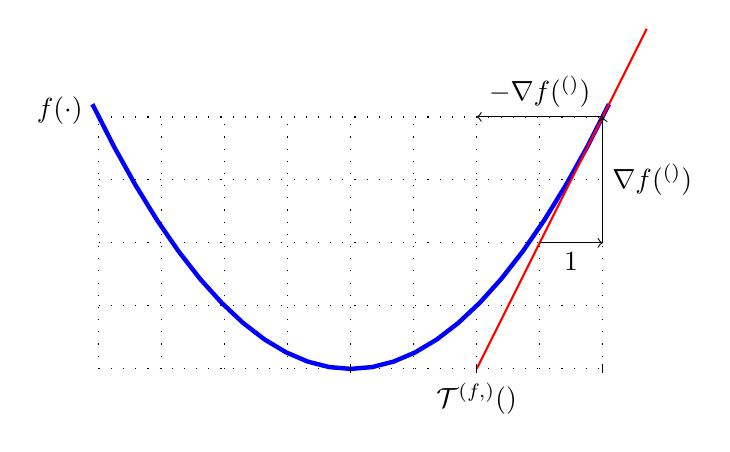
\begin{tikzpicture}[scale=0.8]
					\draw[loosely dotted] (-4,0) grid (4,4);
					\draw[blue, ultra thick, domain=-4.1:4.1] plot (\x,  {(1/4)*\x*\x});
					\draw[red, thick, domain=2:4.7] plot (\x,  {2*\x - 4});
					\draw[<-] (4,4) -- node[right] {$\nabla f(\weights^{(\itercntr)})$} (4,2);
					\draw[->] (4,4) -- node[above] {$-\lrate \nabla f(\weights^{(\itercntr)})$} (2,4);
					\draw[<-] (4,2) -- node[below] {$1$} (3,2) ;
					%\draw[->] (-4.25,0) -- (4.25,0) node[right] {$a$};
					\node[left] at (-4.1, 4.1) {$f(\cdot)$}; 
					\draw[shift={(0,0)}] (0pt,2pt) -- (0pt,-2pt) node[below] {$\overline{\weights}$};
					\draw[shift={(4,0)}] (0pt,2pt) -- (0pt,-2pt) node[below] {$\weights$};
					\draw[shift={(2,0)}] (0pt,2pt) -- (0pt,-2pt) node[below] {$\mathcal{T}^{(f,\lrate)}(\weights)$};
				\end{tikzpicture}
			\end{center}
			\caption{Der grundlegende \gls{gradient} enschjritt \eqref{equ_def_gd_basic_dict}  bildet einen gegebenen Vektro  $\weights$ 
				auf den aktualisierten Vektor $\weights'$ ab. Er definiert einen Operator,
				$\mathcal{T}^{(f,\lrate)}(\cdot): \mathbb{R}^{\nrfeatures} \rightarrow \mathbb{R}^{\nrfeatures}:
				\weights \mapsto \widehat{\weights}$.}
			\label{fig_basic_GD_step_single_dict}
		\end{figure}
		Beachte das der  \gls{gradient}enschritt \eqref{equ_def_gd_basic_dict} lokal optimisiert - in einer \gls{neighborhood}, deren Größe durch die  \gls{stepsize} $\lrate$, eine lineare Annäherung an die Funktion $f(\cdot)$ bestimmt wird.  
		Eine naheliegende  \gls{Verallgemeinerung} 
		von \eqref{equ_def_gd_basic_dict} besteht darin, die Funktion selbst, statt der linearen Annäherung,  lokal zu optimieren, sodass:
		
		\begin{align} 
			\label{equ_approx_gd_step_dict}
			\widehat{\weights} = \argmin_{\weights' \in \mathbb{R}^{\dimlocalmodel}} f(\weights')\!+\!(1/\lrate)\normgeneric{\weights-\weights'}{2}^2. 
		\end{align}
		Wir verwenden absichtlich das gleiche Symbol $\lrate$ wie in \eqref{equ_def_gd_basic_dict}, 
		da auch hier gilt: Je größer $\lrate$, desto größer typischerweise der Fortschritt hin zu 
		einem kleineren Funktionswert $f(\widehat{\weights})$. Ähnlich wie der Gradientenschritt 
		\eqref{equ_def_gd_basic_dict} definiert auch die Aktualisierung \eqref{equ_approx_gd_step_dict} 
		einen (typischerweise nichtlinearen) Operator, der durch die Funktion $f(\cdot)$ und den Parameter 
		$\lrate$ bestimmt ist. Für eine \gls{konvexe} Funktion $f(\cdot)$ ist dieser Operator auch als 
		\gls{proxop} der Funktion bekannt \cite{ProximalMethods}.
		},
		first={Gradientenschritt},text={Gradientenschritt},plural={Gradientenschritte}
}

\newglossaryentry{operator} 
{
    name={Operator}, 
    description={Ein\index{Operator} Operator ist eine \gls{function}, 
        deren \gls{domain} und \gls{co-domain} eine spezifische mathematische Struktur aufweisen, 
        wie z. B. ein \gls{vectorspace}, \gls{hilbertspace} oder \gls{metricspace} \cite{Bauschke:2017,DunfordSchwartz1988}. 
        Viele \gls{ml}-Methoden arbeiten mit Operatoren, deren \gls{domain} und \gls{co-domain} 
        ein \gls{euclidspace} sind.
        \\
        Siehe auch: \gls{vectorspace}, \gls{function}, \gls{hilbertspace}.},
    first={Operator},
    type=math, 
    plural={Operatoren},
    firstplural={Operatoren},
    text={Operator}
}


\newglossaryentry{contractop}
{name={contraction operator},
	description={An\index{contraction operator} operator $\fixedpointop: \mathbb{R}^{\nrfeatures} \rightarrow \mathbb{R}^{\nrfeatures}$
		is a contraction if, for some $\contractfac \in [0,1)$,
		\begin{equation} 
			\nonumber
			\normgeneric{ \fixedpointop \weights\!-\!\fixedpointop \weights'}{2}  \leq  \contractfac	\normgeneric{\weights\!-\!\weights'}{2} \mbox{ holds for any } \weights,\weights' \in \mathbb{R}^{\nrfeatures}.
		\end{equation}
	},
	first={contraction operator},
	text={contraction operator}, 
	firstplural={contraction operators}, 
	plural={contraction operators}
}


\newglossaryentry{proxop}
{name={Proximaloperator},
	description={Gegeben sei \index{proximal operator} eine \gls{convex}e Funktion $f(\weights')$. Wir definieren ihren Proximal Operator gemäß \cite{ProximalMethods}, \cite{Bauschke:2017} als: 
		$$\proximityop{f(\cdot)}{\weights}{\rho}\defeq \argmin_{\weights' \in \mathbb{R}^{\dimlocalmodel}} \bigg[ f(\weights')\!+\!(\rho/2) \normgeneric{\weights- \weights'}{2}^{2}\bigg] \mbox{ mit } \rho > 0. $$ 
		Wie in Fig. \ref{fig_proxoperator_opt_dict}  illustriert, entspricht die Auswertung des Proximaloperators der Minimierung einer penalisierten Variante von $f(\weights')$. Der Strafterm ist der skalierte quadratische euklidische Abstand zu einem gegebenen Vektor $\weights$ (welcher der Eingabewert des Proximaloperators ist).
	
		%\Gls{convex} functions for which the proximal operator can be computed efficiently 
		%is sometimes referred to as \emph{proximable} or \emph{simple} \cite{Condat2013}. 
		Der Proximaloperator kann als eine \gls{generalization} des e \gls{gradstep}s interpretiert werden, der für eine \gls{smooth} \gls{convex}e Funktion  $f(\weights') $ definiert ist. Tatsächlich entspricht ein
		\gls{gradstep} mit \gls{stepsize} $\lrate$ am momentanen Vektor r $\weights$ der Anwendung des Proximaloperators der Funktion 
		 $\tilde{f}(\weights')= \big( \nabla f(\weights)\big)^{T} (\weights'-\weights)$ 
		mit $\rho=1/\lrate$.
		\begin{figure}[H]
			\begin{center}
				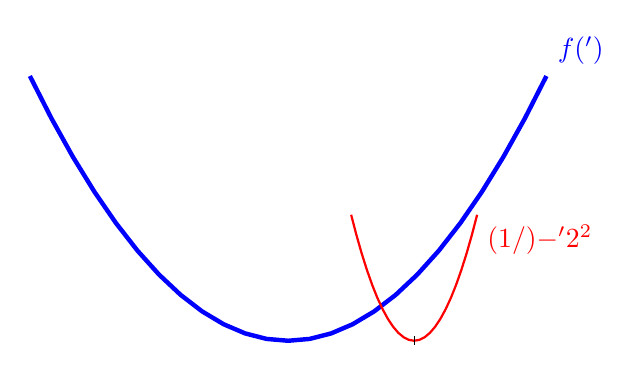
\begin{tikzpicture}[scale=0.8]
					% Original quadratic function
					\draw[blue, ultra thick, domain=-4.1:4.1] plot (\x, {(1/4)*\x*\x}) node[above right] {$f(\weights')$};		
					% Quadratic function with larger curvature, centered at w = 2
					\draw[red, thick, domain=1:3] plot (\x, {2*(\x - 2)*(\x - 2)}) node[below right] {$(1/\lrate)\normgeneric{\weights-\weights'}{2}^{2}$};
					% Axes
					% Minimum point of second curve
					\draw[shift={(2,0)}] (0pt,2pt) -- (0pt,-2pt) node[below] {$\weights$};
					%\node at (2,0.5) [anchor=north] {$\weights$};
				\end{tikzpicture}
			\end{center}
			\caption{A generalized \gls{gradstep} updates a vector $\weights$ by minimizing a penalized version 
				of the function $f(\cdot)$. The penalty term is the scaled squared Euclidean distance between the optimization 
				variable $\weights'$ and the given vector $\weights$.	\label{fig_proxoperator_opt_dict}}
		\end{figure}
	},first={proximal operator},text={proximal operator}}
}

	
\newglossaryentry{proximable}
{
    name={proximierbar},
    description={Eine\index{proximierbar} \gls{convex} \gls{function}, für die der \gls{proxop} effizient berechnet werden kann, 
        wird manchmal als proximierbar oder einfach bezeichnet \cite{Condat2013}.
        \\
        Siehe auch: \gls{convex}, \gls{function}, \gls{proxop}.},
    first={proximierbar},
    text={proximierbar}
}


\newglossaryentry{connected}
{
    name={zusammenhängend}, 
    description={Ein\index{zusammenhängend} \gls{undirectedgraph} $\graph=\pair{\nodes}{\edges}$ 
        ist zusammenhängend, wenn für jede nicht-leere Teilmenge $\nodes' \subset \nodes$ 
        mindestens eine Kante existiert, die einen Knoten in $\nodes'$ mit einem Knoten in $\nodes \setminus \nodes'$ verbindet.
        \begin{figure}[H]
        \centering
        \begin{tikzpicture}
        % Linkes Diagramm (nicht zusammenhängend)
        \node[circle, fill=black, inner sep=1.5pt, label=above:{1}] (A1) at (0, 1.5) {};
        \node[above=0.5cm of A1, align=center] {nicht zusammenhängend};
        \node[circle, fill=black, inner sep=1.5pt, label=below right:{2}] (B1) [below right=0.8cm and 0.5cm of A1] {};
        \node[circle, fill=black, inner sep=1.5pt, label=below left:{3}] (C1) [below left=0.8cm and 0.5cm of A1] {};
        \draw [line width=1 pt]  (A1) -- (B1);
        % Rechtes Diagramm (zusammenhängend)
        \begin{scope}[xshift=3.5cm]
            \node[circle, fill=black, inner sep=1.5pt, label=above:{1}] (A2) at (0, 1.5) {};
            \node[above=0.5cm of A2, align=center] {zusammenhängend};
            \node[circle, fill=black, inner sep=1.5pt, label=below right:{2}] (B2) [below right=0.8cm and 0.5cm of A2] {};
            \node[circle, fill=black, inner sep=1.5pt, label=below left:{3}] (C2) [below left=0.8cm and 0.5cm of A2] {};
            \draw [line width=1 pt]  (A2) -- (B2);
            \draw [line width=1 pt]  (B2) -- (C2);
        \end{scope}
        \end{tikzpicture}
        \end{figure} 
        Siehe auch: \gls{undirectedgraph}, \gls{algconn}.}, 
    type=math, 
    first={zusammenhängend},
    text={zusammenhängend}
}


\newglossaryentry{mvndist}
{
    name={multivariate Normalverteilung}, 
    description={Die\index{multivariate Normalverteilung} multivariate Normalverteilung, 
        die mit $\mvnormal{\meanvecgeneric}{\covmtxgeneric}$ bezeichnet wird, ist ein fundamentales 
        \gls{probmodel} für numerische \glspl{featurevec} fester Dimension $\nrfeatures$. 
        Sie definiert eine Familie von \glspl{probdist} über \gls{vector}-wertige \glspl{rv} 
        $\featurevec \in \mathbb{R}^{\nrfeatures}$~\cite{BertsekasProb,GrayProbBook,Lapidoth09}. 
        Jede Verteilung aus dieser Familie wird vollständig durch ihren \gls{mean}-\gls{vector} 
        $\meanvecgeneric \in \mathbb{R}^{\nrfeatures}$ und ihre \gls{covmtx} 
        $\covmtxgeneric \in \mathbb{R}^{\nrfeatures \times \nrfeatures}$ bestimmt. 
        Wenn die \gls{covmtx} $\covmtxgeneric$ invertierbar ist, wird die entsprechende 
        \gls{probdist} durch die folgende \gls{pdf} beschrieben:
        \[
        p(\featurevec) = 
        \frac{1}{\sqrt{(2\pi)^{\nrfeatures} \det\,(\covmtxgeneric)}} 
        \exp\Big[ -\frac{1}{2} 
        (\featurevec - \meanvecgeneric)\,^{T}\, \covmtxgeneric^{-1} 
        (\featurevec - \meanvecgeneric) \Big].
        \]
        Diese \gls{pdf} ist nur definiert, wenn $\covmtxgeneric$ invertierbar ist.
        Allgemeiner gilt für jede \gls{rv} $\featurevec \sim \mvnormal{\meanvecgeneric}{\covmtxgeneric}$ die Darstellung:
        \[
        \featurevec = \mA \vz + \meanvecgeneric,
        \]
        wobei $\vz \sim \mvnormal{\mathbf{0}}{\mathbf{I}}$ ein \gls{stdnormvec} ist und 
        $\mA \in \mathbb{R}^{\nrfeatures \times \nrfeatures}$ die Bedingung $\mA \mA^\top = \covmtxgeneric$ erfüllt. 
        Diese Darstellung bleibt auch gültig, wenn $\covmtxgeneric$ singulär ist, wobei $\mA$ in diesem Fall 
        nicht vollrangig ist~\cite[Ch. 23]{Lapidoth2017}.
        Die Familie der multivariaten Normalverteilungen ist unter \glspl{probmodel} für numerische 
        Größen besonders, insbesondere aus folgenden Gründen. Erstens ist die Familie abgeschlossen unter affinen 
        Transformationen, d.h.,
        \[
        \featurevec \sim \mathcal{N}(\meanvecgeneric,\covmtxgeneric) \implies 
        \mB\featurevec\!+\!\vc \sim \mathcal{N}\big( \mB\meanvecgeneric+\vc,\mB \covmtxgeneric \mB\,^{T} \big). 
        \]
        Zweitens maximiert die \gls{probdist} $\mathcal{N}(\mathbf{0},\covmtxgeneric)$ die 
        \gls{diffentropy} unter allen Verteilungen mit derselben \gls{covmtx} $\covmtxgeneric$~\cite{coverthomas}. 
        \\ 
        Siehe auch: \gls{probmodel}, \gls{probdist}, \gls{stdnormvec}, \gls{diffentropy}, \gls{gaussrv}.}, 
    first={multivariate Normalverteilung},
    text={multivariate Normalverteilung}
}



\newglossaryentry{stdnormvec}
{name={standard normal vector}, 
	description={A\index{standard normal vector} standard normal \gls{vector} is a random 
		\gls{vector} $\vx=\big(x_{1}, \ldots, x_{\nrfeatures}\big)\,^{T}$ 
		whose entries are \gls{iid} \glspl{gaussrv} $x_{\featureidx} \sim \mathcal{N}(0,1)$. 
		It is a special case of a \gls{mvndist}, $\vx \sim \mathcal(\mathbf{0},\mathbf{I})$.
		\\ 
		See also: \gls{vector}, \gls{iid}, \gls{gaussrv}, \gls{mvndist}, \gls{rv}.}, 
	first={standard normal vector},
	text={standard normal vector}
}


\newglossaryentry{earlystopping}
{
    name={Early Stopping}, 
    description={Betrachten wir eine auf \gls{erm} basierende Methode, die ein 
        iteratives \gls{optmethod} (z.\,B. \gls{gd}) verwendet, um \glspl{modelparam} 
        durch Minimierung des \gls{emprisk} auf einem gegebenen \gls{trainset} zu lernen. 
        Early Stopping \index{early stopping} bezeichnet das vorzeitige Beenden der Iterationen, 
        selbst wenn diese das \gls{emprisk} auf dem \gls{trainset} noch deutlich verringern würden. 
        Anstatt die \gls{objfunc} (also den \gls{emprisk} auf dem \gls{trainset}) zu überwachen, 
        wird beim Early Stopping die \gls{valerr} verfolgt, die von den \glspl{modelparam} in jeder Iteration 
        verursacht wird. Early Stopping kann als eine Implementierung von \gls{regularization} 
        über das Beschneiden des \gls{model} interpretiert werden. Tatsächlich schränkt das Beenden 
        eines iterativen \gls{optmethod} nach nur wenigen Iterationen die Menge der \glspl{modelparam} 
        ein, die von der Initialisierung aus erreichbar sind (siehe Abb.\ \ref{fig_early_stopping_dict}).
        \begin{figure}[htbp]
        \centering
            \begin{tikzpicture}[>=Stealth, scale=2]
            % Initialisierung
            \fill (0,0) circle (0.6pt) node[above] {\small $\weights^{(0)}$};
            \node at (-0.4,0) {\small $\hypospace^{(1)}$};
            \node at (-1.2,0) {\small $\hypospace^{(2)}$};
            \node at (-2,0) {\small $\hypospace \ldots$};
            % Erreichbare T-Schritte (Early Stopping = kleineres T)
            \draw[densely dotted] (0,0) ellipse (0.8 and 0.4);
            \draw[dashed] (0,0) ellipse (1.6 and 0.8);
            % Beispielpfad des Gradienten (nur illustrativ)
            \draw[->] (0,0) -- (0.8,0.) node [pos=0.6,above] {\tiny $1$ Schritt};
            \draw[->] (0.0,0.0) -- (0,-0.8) node [pos=0.9,right] {\tiny $2$ Schritte};
            \end{tikzpicture}
            \caption{Ein \gls{gdmethod} für \gls{erm} unter Verwendung eines \gls{hypospace} $\hypospace$ 
                definiert eine verschachtelte \gls{sequence} effektiver \glspl{hypospace} 
                $\hypospace^{(1)} \subseteq \hypospace^{(2)} \subseteq \ldots \subseteq \hypospace$. 
                Der effektive \gls{hypospace} $\hypospace^{(\iteridx)}$ wird durch alle \glspl{modelparam} 
                bestimmt, die von der Initialisierung $\weights^{(0)}$ innerhalb von $\iteridx$ \glspl{gradstep} 
                erreichbar sind. \label{fig_early_stopping_dict}}
            \end{figure} \\ 
        Siehe auch: \gls{gdmethod}, \gls{regularization}, \gls{overfitting}.},
    first={Early Stopping},
    text={Early Stopping}
}


 \newglossaryentry{statasp}
		 {name ={statistische Aspekte}, 
		 	description={Unter statistischen Aspekten\index{statistical aspects} einer  \gls{ml}-Methode versteht man (Eigenschaften) der \gls{probdist}
		 		seiner Ausgabe unter einem a \gls{probmodel} für die  \gls{data}, die in das Verfahren eingespeisst werden.},
		 		first={Statistische Aspekte},text={statistische Aspekte}}

\newglossaryentry{compasp}
{name={rechnerische Aspekte},
	description={Unter rechnerischen Aspekten \index{computational aspects} eines \gls{ml}-Verfahrens verstehen wir hauptsächlich die für dessen Implementierung erforderlichen Rechenressourcen. Zum Beispiel umfasst bei einem \gls{ml}-Verfahren, das iterative Optimierungstechniken zur Lösung von \gls{erm} verwendet, die computational aspects: 1) wie viele arithmetische Operationen für eine einzelne Iteration (d.h. einen \gls{gradstep}) benötigt werden; und 2) wie viele Iterationen erforderlich sind, um nützliche \glspl{modelparam} zu erhalten. Ein wichtiges Beispiel für eine iterative Optimierungstechnik ist \gls{gd}.},
	first={Rechnerische Aspekte},
	text={rechnerische Aspekte}
}

\newglossaryentry{zerooneloss}
{
    name={$\bf 0/1$ loss},
    sort={zerooneloss}, 
    description={Der $0/1$ \gls{loss}\index{$0/1$ loss} 
        $\lossfunczo{\pair{\featurevec}{\truelabel}}{\hypothesis}$ bewertet die Qualität 
        eines \gls{classifier} $\hypothesis(\featurevec)$, der eine \gls{prediction} 
        $\predictedlabel$ (z.\,B. durch Thresholding \eqref{equ_def_threshold_bin_classifier_dict}) 
        für das \gls{label} $\truelabel$ eines \gls{datapoint} mit \glspl{feature} $\featurevec$ liefert. 
        Der Verlust ist $0$, wenn die \gls{prediction} korrekt ist, d.\,h. 
        $\lossfunczo{\pair{\featurevec}{\truelabel}}{\hypothesis}=0$ für 
        $\predictedlabel=\truelabel$, und $1$, wenn die \gls{prediction} falsch ist, d.\,h. 
        $\lossfunczo{\pair{\featurevec}{\truelabel}}{\hypothesis}=1$ für 
        $\predictedlabel\neq\truelabel$.
        \\ 
        Siehe auch: \gls{loss}, \gls{classifier}, \gls{prediction}, \gls{label}, \gls{datapoint}, \gls{feature}.},
    first={$0/1$ loss},
    text={$0/1$ loss}
}

		 
\newglossaryentry{probability}
{name={Wahrscheinlichkeit},
	description={Wir\index{probability} ordnen jedem Ereignis, das bei einem Zufallsexperiment auftreten kann, 
	einen Wahrscheinlichkeitswert zu, der typischerweise im 
	Intervall $[0,1]$ liegt \cite{BertsekasProb}, \cite{HalmosMeasure}, \cite{BillingsleyProbMeasure}, \cite{KallenbergBook}.},
	first={Wahrscheinlichkeit},
	text={Wahrscheinlichkeit}
	plural={Wahrscheinlichkeiten}
}

\newglossaryentry{underfitting}
{name={Unteranpassung},
	description={Betrachten wir eine \gls{ml}-Methode, die \gls{erm} verwendet, um eine \gls{hypothesis} mit dem
	 minimalen \gls{emprisk} auf einem gegebenen \gls{trainset} zu lernen. Eine solche Methode unterfitttet 
	 das \gls{trainset}, wenn sie nicht in der Lage ist, eine \gls{hypothesis} mit ausreichend kleinem \gls{emprisk} 
	 auf dem \gls{trainset} zu lernen. Wenn eine Methode Unteranpassung aufweist, ist sie typischerweise auch nicht 
	 in der Lage, eine \gls{hypothesis} mit kleinem \gls{risk} zu lernen.},
	first={Unteranpassung},
	text={Unteranpassung}
}


\newglossaryentry{overfitting}
{name={Überanpassung}},
	description={Betrachten wir eine \gls{ml}-Methode, die \gls{erm} verwendet, um eine \gls{hypothesis} mit 
	dem minimalen \gls{emprisk} auf einem gegebenen \gls{trainset} zu lernen. Eine solche Methode ist überangepasst
	 an das \gls{trainset}, wenn sie eine \gls{hypothesis} mit kleinem \gls{emprisk} auf dem \gls{trainset} lernt,
	  aber außerhalb des \gls{trainset} einen deutlich größeren \gls{loss} aufweist.},
	first={Überanpassung},
	text=Überanpassung}
                        
    }

\newglossaryentry{gdpr}
{name={Datenschutz-Grundverordnung (DSGVO)},
	description={Die\index{Datenschutz-Grundverordnung (DSGVO)} DSGVO\cite{GDPR2016} 
			wurde von der Europäischen Union (EU) erlassen und trat am 25. Mai 2018 in Kraft \cite{GDPR2016}. 
			Sie ist ein strenges Datenschutz- und Sicherheitsgesetz, das den Schutz der Privatsphäre von Einzelpersonen gewährleistet und die Verarbeitung personenbezogener Daten regelt.
			Die DSGVO ist technologieneutral, wirkt sich jedoch auf die Verarbeitung und Nutzung von Daten im Kontext von maschinellem Lernen aus: 
			 
			Grundsätze der Verarbeitung personenbezogener Daten (Artikel 5 DSGVO)
			\begin{itemize}
				\item{Rechtmäßigkeit, Verarbeitung nach Treu und Glauben, Transparenz} - \gls{data} müssen rechtmäßig, nach Treu und Glauben und transparent verarbeitet werden.
				\item \Gls{dataminprinc}: \gls{ml}-Systeme sollten nur die für den jeweiligen Zweck erforderliche Menge an personenbezogenen 
				\gls{data} verwenden.
				\item{Zweckbindung}: Personenbezogene \gls{data} dürfen nur für einen vorher definierten und kommunizierten Zweck erhoben werden. 
				\item{Speicherbegrenzung}: Personenbezogene \gls{data} dürfen nur so lange aufbewahrt werden, wie es notwendig oder gesetzlich vorgeschrieben ist, und müssen anschließend gelöscht werden. 
				\item{Richtigkeit}: Personenbezogene \gls{data} müssen aktuell und korrekt gehalten werden.
				\item \Gls{data} Betroffenenrechte: Nutzende sollten die Möglichkeit erhalten, auf ihre personenbezogenen \gls{data} zuzugreifen, sie zu berichtigen und zu löschen sowie der automatisierten Entscheidungsfindung und Profilbildung zu widersprechen.
				\item{Integrität und Vertraulichkeit}: Personenbezogene \gls{data} müssen sicher verarbeitet und vor unbefugter Verarbeitung, Verlust oder Zerstörung geschützt werden. 
			\end{itemize}
			
		Zusätzlich gewährt die DSGVO den Betroffenen das Recht auf Information, Zugang und Berichtigung ihrer Daten, das Recht auf Löschung („Recht auf Vergessenwerden“), Einschränkung
		 der Verarbeitung, Datenübertragbarkeit sowie das Widerspruchsrecht gegen die Verarbeitung. Schließlich definiert die DSGVO das Recht, nicht einer ausschließlich automatisierten
		  Entscheidung unterworfen zu werden (Artikel 22 DSGVO) sowie das Recht auf Erläuterung automatisierter Entscheidungen und menschliche Aufsicht. 
		Siehe auch: \gls{data}, \gls{ml}, \gls{dataminprinc}, \gls{transparency}, \gls{explainability}.}, 
	first={Datenschutz-Grundverordnung (DSGVO)},
	text={DSGVO}
}

	
\newglossaryentry{gaussrv}{
	name={Gaußsche Zufallsvariable (Gaußsche ZV)},
	description={
		Eine \index{Gaußsche Zufallsvariable (Gaußsche ZV)} standard-Gaußsche \gls{rv} ist eine 
		reellwertige \gls{rv} $x$ mit der \gls{pdf} \cite{BertsekasProb}, \cite{GrayProbBook}, \cite{papoulis}
		\begin{equation}
			\nonumber
			p(x) = \frac{1}{\sqrt{2\pi}} \exp^{-x^2/2}.
		\end{equation}
		Ausgehend von einer standard-Gaußschen \gls{rv} $x$ lässt sich eine allgemeine Gaußsche \gls{rv} $x'$ 
		mit \gls{mean} $\mu$ und \gls{variance} $\sigma^2$ durch $x' \defeq \sigma (x + \mu)$ konstruieren. 
		Die \gls{probdist} einer Gaußschen \gls{rv} wird als Normalverteilung bezeichnet und mit 
		$\mathcal{N}(\mu, \sigma)$ notiert. \\ 
		Ein Gaußscher Zufallsvektor $\featurevec \in \mathbb{R}^{\featuredim}$ mit 
		\gls{covmtx} $\mathbf{C}$ und \gls{mean} ${\bm \mu}$ kann durch 
		$\featurevec \defeq \mathbf{A} \big( \vz + {\bm \mu} \big)$ erzeugt werden. 
		Dabei ist $\mA$ eine Matrix, die $\mA\mA^{T} = \mC$ erfüllt, 
		und $\vz \defeq \big( z_{1},\ldots,z_{\featuredim} \big)^{T}$ ist ein Vektor, dessen Einträge 
		\gls{iid} standard-Gaußsche \gls{rv}s $z_{1},\ldots,z_{\featuredim}$ sind. \\
		Gaußsche Zufallsvektoren sind ein Spezialfall von Gaußschen Prozessen, 
		die als lineare Transformationen unendlicher Folgen von standard-Gaußschen \gls{rv}s 
		aufgefasst werden können \cite{Rasmussen2006Gaussian}. \\
		Gaußsche \gls{rv}s sind weit verbreitete \gls{probmodel}s in der statistischen Analyse 
		von \gls{ml}-Methoden. Ihre Bedeutung ergibt sich unter anderem aus dem zentralen Grenzwertsatz, 
		welcher besagt, dass der Mittelwert einer wachsenden Anzahl unabhängiger \gls{rv}s 
		(die selbst nicht notwendigerweise gaußverteilt sind) gegen eine Gaußsche \gls{rv} konvergiert 
		\cite{ross2013first}. \\
		Siehe auch: \gls{probdist}, \gls{probdist}, \gls{probspace}.
	},
	first={Gaußsche Zufallsvariable (Gaußsche ZV)},
	text={Gaußsche ZV}
}
\newglossaryentry{normaldist} 
{name={Normalverteilung}, 
 description={Siehe\index{Normalverteilung} \gls{gaussrv}.},
 first={Normalverteilung}, 
 firstplural={Normalverteilungen},
 plural={Normalverteilungen},
 type=math, 
 text={Normalverteilung}
}


    	
\newglossaryentry{clt}
{name={central limit theorem (CLT)},
	description={Consider a sequence of \gls{iid} \glspl{rv} \( \feature^{(\sampleidx)} \), for \( \sampleidx = 1, 2, \ldots \), 
		each with \gls{mean} zero and finite \gls{variance} \( \sigma^2 > 0 \). 
		The \index{central limit theorem (CLT)} CLT states that the normalized sum 
		\[
		s^{(\samplesize)} \defeq \frac{1}{\sqrt{\samplesize}} \sum_{\sampleidx = 1}^{\samplesize} \feature^{(\sampleidx)} 
		\]
		converges in distribution to a \gls{gaussrv} with \gls{mean} zero and \gls{variance} \( \sigma^2 \) as \( \samplesize \to \infty \) \cite[Proposition~2.17]{AsympVanderVaartBook}.
		One elegant way to derive the CLT is via the \gls{characteristicfunc} of the normalized sum \( s^{(\samplesize)} \). 
		Let $ \phi(t) = \expect \big\{ \exp \big( j t \feature \big) \big\}$ (with the imaginary unit $j = \sqrt{-1}$) 
		be the common \gls{characteristicfunc} of each sum and $\feature^{(\sampleidx)}$, and let \( \phi^{(\samplesize)}(t) \) 
		denote the \gls{characteristicfunc} of \( s^{(\samplesize)} \). Define an operator \( \mathcal{T} \) acting on \glspl{characteristicfunc} 
		such that
		\[
		\phi^{(\samplesize)}(t) = \mathcal{T}(\phi^{(\samplesize-1)})(t) \defeq \phi\left( \frac{t}{\sqrt{\samplesize}} \right) \cdot \phi^{(\samplesize-1)}\left( \frac{\sqrt{\samplesize-1}}{\sqrt{\samplesize}} t \right).
		\]
		This \gls{fixedpointiter} captures the effect of recursively adding an \gls{iid} \gls{rv} $\featurevec^{(\samplesize)}$ 
		and rescaling. Iteratively applying \( \mathcal{T} \) leads to convergence of \( \phi^{(\samplesize)}(t) \) toward the fixed point
		\[
		\phi^*(t) = \exp\,(-t^2 \sigma^2 / 2)
		\]
		which is the \gls{characteristicfunc} of a \gls{gaussrv} with \gls{mean} zero and \gls{variance} 
		\( \sigma^2 \). \Glspl{generalization} of the CLT allow for dependent or non-identically distributed \glspl{rv} \cite[Sec.~2.8]{AsympVanderVaartBook}.
		\begin{figure}[H]
			\centering
			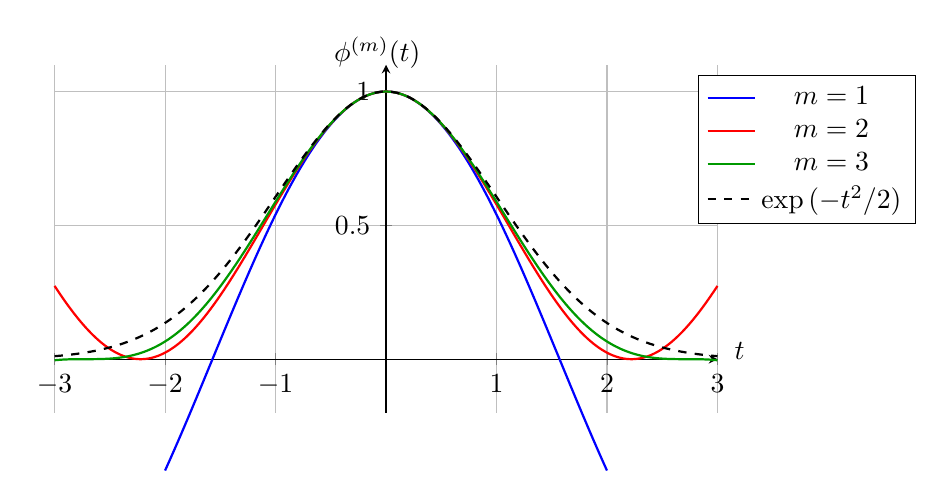
\begin{tikzpicture}
			\begin{axis}[
			width=10cm,
			height=6cm,
			xlabel={},
			ylabel={},
			legend style={at={(0.97,0.97)}, anchor=north west},
			domain=-3:3,
			ylabel style={
			yshift=10pt   % shift label up by 10pt
			},
			samples=400,
			ymin=-0.2, ymax=1.1,
			axis lines=middle,
			clip=false,
			grid=both,
			]
			\addplot[thick, blue,domain=-2:2] {cos(x/sqrt(1) r)^1};
			\addlegendentry{$m=1$}
			\addplot[thick, red] {cos(x/sqrt(2) r)^2};
			\addlegendentry{$m=2$}
			\addplot[thick, green!60!black] {cos(x/sqrt(3) r)^3};
			\addlegendentry{$m=3$}
			\addplot[thick, dashed, black] {exp(-x^2/2)};
			\addlegendentry{$\exp\,(-t^2/2)$}
			\node[anchor=south, rotate=0] at (axis cs:-0.08,1.05) {$\phi^{(m)}(t)$};
			\node[anchor=north, rotate=0] at (axis cs: 3.2,0.1) {$t$};
			\end{axis}
			\end{tikzpicture}
			\caption{\Glspl{characteristicfunc} of normalized sums of \gls{iid} \glspl{rv} $x^{(\sampleidx)} \in \{-1,1\}$ 
			for $\sampleidx=1,\ldots,\samplesize$ compared to the Gaussian limit.}
		\end{figure}
		See also: \gls{rv}, \gls{gaussrv}.},
	first={central limit theorem (CLT)},
	text={CLT}
}

\newglossaryentry{GaussProc}
{name={Gauß-Prozess (GP)},
	description={Ein \index{Gauß-Prozess (GP)}Gauß-Prozess ist eine Familie von \gls{rv}s 
		$\{f(\featurevec)\}_{\featurevec \in \featurespace}$, die durch Eingabewerte $\featurevec$ 
		aus einem Eingaberaum $\featurespace$ indiziert sind. Für jede endliche Teilmenge 
		$\featurevec^{(1)}, \ldots, \featurevec^{(\samplesize)} \in \featurespace$ 
		haben die entsprechenden \gls{rv}s $f(\featurevec^{(1)}), \ldots, f(\featurevec^{(\samplesize)})$ 
		eine gemeinsame multivariate Normalverteilung:
		\[
		\left( f(\featurevec^{(1)}), \ldots, f(\featurevec^{(\samplesize)}) \right) \sim \mathcal{N}(\boldsymbol{\mu}, \mathbf{K}).
		\]
		Für einen festen Eingaberaum $\featurespace$ ist ein Gauß-Prozess vollständig definiert durch:
		\begin{itemize}
			\item eine \gls{mean}-Funktion $\mu(\featurevec) = \expect\{ f(\featurevec)\}$,
			\item und eine Kovarianzfunktion $\kernelmap{\featurevec}{\featurevec'}= \expect\{ \big(f(\featurevec)-\mu(\featurevec)\big) \big(f(\featurevec')-\mu(\featurevec')\big) \big\}$.
		\end{itemize}
		\textbf{Beispiel.} Die Temperaturverteilung über Finnland zu einem bestimmten Zeitpunkt kann als \gls{realization} eines Gauß-Prozesses $f(\featurevec)$ interpretiert werden, wobei jeder Eingabewert $\featurevec = (\text{lat}, \text{lon})$ eine geografische Position darstellt. Temperaturmessungen von \gls{fmi}-Wetterstationen liefern Stichproben von $f(\featurevec)$ an bestimmten Orten (siehe Abb.\ \ref{fig_gp_FMI}). Ein Gauß-Prozess ermöglicht es, die Temperatur in der Nähe von \gls{fmi}-Wetterstationen vorherzusagen und die Unsicherheit dieser Vorhersagen zu quantifizieren.
		\begin{figure}[H]
			\begin{center}
				\begin{tikzpicture}
					\begin{axis}[
						axis equal,
						hide axis,
						scale=1.2,
						xmin=17, xmax=32,
						ymin=55, ymax=71,
						clip=true
						]
						% --- Finnland-Grenze (Polylinie) ---
						\addplot[
						color=black,
						thick
						] table [x=lon, y=lat, col sep=comma] {assets/finland_border.csv};
						% --- FMI-Messstationen ---
						\addplot[
						only marks,
						mark=*,
						mark options={fill=blue},
						color=black
						] table [x=lon, y=lat, col sep=comma] {assets/fmi_stations_subset.csv};
						% Manuelle Achsen zeichnen
						\draw[->, thick] (axis cs:19,59) -- (axis cs:25.5,59) node[anchor=west] {lon};
						\draw[->, thick] (axis cs:19,59) -- (axis cs:19,65.5) node[anchor=south] {lat};
					\end{axis}
				\end{tikzpicture}
				\vspace*{-15mm}
			\end{center}
			\caption{Die Temperaturverteilung über Finnland kann als \gls{realization} 
				eines Gauß-Prozesses interpretiert werden, der durch geografische Koordinaten indiziert ist und an \gls{fmi}-Wetterstationen (blaue Punkte) abgetastet wird. \label{fig_gp_FMI}}
	\end{figure}},
	first = {Gauß-Prozess},
	text = {GP}
}

	
\newglossaryentry{trustAI}
{name={Vertrauenswürdige Künstliche Intelligenz (trustworthy AI)},
	description={Neben den \gls{compasp}en und \gls{statasp}en gibt es einen dritten 
		Entwurfsaspekt für \gls{ml}-Methoden: Vertrauenswürdigkeit\index{trustworthy AI} 
		\cite{pfau2024engineeringtrustworthyaideveloper}. 
		Die EU hat sieben zentrale Anforderungen (Key Requirements, KRs) für 
		vertrauenswürdige \gls{ai} aufgestellt (die typischerweise auf \gls{ml}-Methoden basieren)
		\cite{ALTAIEU}:
		\begin{enumerate}[label=\arabic*)]
			\item KR1 – Vorrang menschlichen Handelns und menschliche Aufsicht,
			\item KR2 – Technische Robustheit und Sicherheit,
			\item KR3 – Datenschutz und Daten-Governance,
			\item KR4 – Transparenz,
			\item KR5 – Vielfalt, Nichtdiskriminierung und Fairness,
			\item KR6 – Gesellschaftliches und ökologisches Wohlergehen,
			\item KR7 – Rechenschaftspflicht.
		\end{enumerate}
	},
	first={Vertrauenswürdige Künstliche Intelligenz (trustworthy AI)},
	text={Vertrauenswürdige Künstliche Intelligenz}
}
	
\newglossaryentry{sqerrloss}
{name={quadratische Verlustfunktion},
	description={Die quadratische Verlustfunktion \index{quadratische Verlustfunktion} \gls{loss} 
		misst den \gls{prediction}fehler einer \gls{hypothesis} $\hypothesis$ 
		bei der Vorhersage eines numerischen \gls{label}s $\truelabel \in \mathbb{R}$ 
		anhand der \gls{feature}s $\featurevec$ eines \gls{datapoint}. Er ist definiert als
		\begin{equation} 
			\nonumber
			%	\label{equ_squared_loss_gls}
			\lossfunc{(\featurevec,\truelabel)}{\hypothesis} \defeq \big(\truelabel - \underbrace{\hypothesis(\featurevec)}_{=\predictedlabel} \big)^{2}. 
		\end{equation}
	},
	first={quadratische Verlustfunktion},
	text={quadratische Verlustfunktion}
}


\newglossaryentry{projection}
{name={Projektion}, 
	description={Betrachten wir einen Teilsatz $\paramspace \subseteq \mathbb{R}^{\dimlocalmodel}$ 
		des $\dimlocalmodel$-dimensionalen \gls{euclidspace}. Wir definieren die Projektion $\projection{\paramspace}{\weights}$
		eines Vektors $\weights \in \mathbb{R}^{\dimlocalmodel}$ auf $\paramspace$ als
		\begin{equation} 
			\label{equ_def_proj_generic_dict}
			\projection{\paramspace}{\weights} = \argmin_{\weights' \in \paramspace} \normgeneric{\weights - \weights'}{2}. 
		\end{equation}
		Mit anderen Worten: $\projection{\paramspace}{\weights}$ ist der Vektor in $\paramspace$, 
		der $\weights$ am nächsten liegt. Die Projektion ist nur für solche Teilmengen $\paramspace$ wohldefiniert, 
		für die das obige \gls{minimum} existiert \cite{BoydConvexBook}.},
	first={Projektion},
	text={Projektion}
}

\newglossaryentry{projgd}{
	name={projizierter Gradientenabstieg (projizierter GD)},
	description={
		Betrachten wir eine auf \gls{erm} basierende Methode, die ein parametriertes \gls{model} 
		mit einem \gls{paramspace} $\paramspace \subseteq \mathbb{R}^{\dimlocalmodel}$ verwendet. 
		Selbst wenn die \gls{objfunc} von \gls{erm} \gls{smooth} ist, können wir den einfachen 
		\gls{gd} nicht verwenden, da dieser keine Nebenbedingungen für die Optimierungsvariable 
		(also die \glspl{modelparam}) berücksichtigt. \\
		Der projizierte \index{projizierter Gradientenabstieg (projizierter GD)} \gls{gd} erweitert 
		den einfachen \gls{gd}, um solche Nebenbedingungen zu berücksichtigen. 
		Ein einzelner Schritt des projizierten \gls{gd} besteht darin, zunächst einen \gls{gradstep} 
		durchzuführen und anschließend das Ergebnis auf den \gls{paramspace} zurückzuprojezieren.
		\begin{figure}[H]
			\begin{center}
				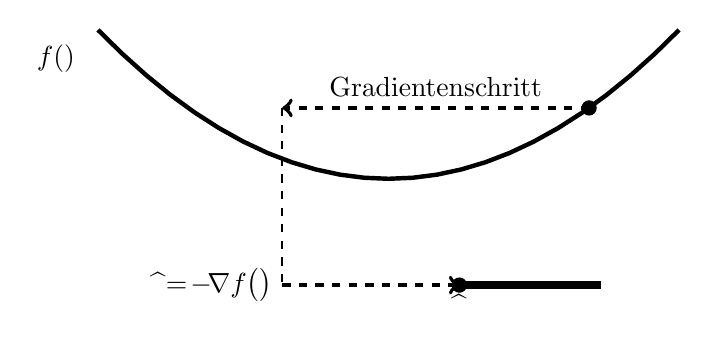
\begin{tikzpicture}[scale=0.9]
					\node [right] at (-5.1,1.7) {$f(\weights)$} ;
					\draw[ultra thick, domain=-4.1:4.1] plot (\x,  {(1/8)*\x*\x});
					\draw [fill] (2.83,1) circle [radius=0.1] node[right] {$\weights$};
					\draw[line width =0.5mm,dashed,->] (2.83,1) -- node[midway,above] {Gradientenschritt} (-1.5,1);
					\draw[line width =0.2mm,dashed] (-1.5,1) --(-1.5,-1.5)  node [below, left]{$\widehat{\weights}=\weights\!-\!\lrate \nabla f\big(\weights\big)$} ;
					\draw[line width =0.5mm,dashed,->] (-1.5,-1.5)  -- node[midway,above] {} (1,-1.5) ; 
					\draw [fill] (1,-1.5) circle [radius=0.1] node[below] {$\projection{\paramspace}{\widehat{\weights}}$};
					\draw[line width=1mm] (1,-1.5) -- (3,-1.5) node[midway, above] {$\paramspace$};
				\end{tikzpicture}
				\vspace*{-5mm}
			\end{center}
			\caption{Projizierter \gls{gd} erweitert einen einfachen \gls{gradstep} durch eine \gls{projection} zurück auf die zulässige Menge $\paramspace$.}
			\label{fig_projected_GD_dict}
		\end{figure}
	},
	first={projizierter Gradientenabstieg (projizierter GD)},
	text={projizierter GD}
}

\newglossaryentry{diffpriv}{
	name=differenzielle Privatsphäre (DP),
	description={
		Betrachten wir eine \gls{ml}-Methode $\algomap$, 
		die ein \gls{dataset} (z.\,B.\ das \gls{trainset} im Rahmen von \gls{erm}) einliest 
		und ein Ergebnis $\algomap(\dataset)$ liefert. Dieses Ergebnis kann entweder aus den 
		gelernten \glspl{modelparam} oder den \gls{prediction}s für bestimmte \gls{datapoint}s bestehen. \\
		Die differenzielle \index{differenzielle Privatsphäre (DP)} Privatsphäre (DP) ist ein präzises Maß 
		für die \gls{privleakage}, die durch die Offenlegung dieses Ergebnisses entsteht. 
		Grob gesagt ist eine \gls{ml}-Methode dann differentielle privat, wenn sich die 
		\gls{probdist} des Ausgabewerts $\algomap(\dataset)$ nicht wesentlich ändert, 
		wenn das \gls{sensattr} eines einzelnen \gls{datapoint} im \gls{trainset} verändert wird. \\
		Wichtig ist, dass DP auf einem \gls{probmodel} der \gls{ml}-Methode basiert – 
		das heißt, wir interpretieren $\algomap(\dataset)$ als \gls{realization} einer \gls{rv}. 
		Die notwendige Zufälligkeit im Ergebnis kann durch gezieltes Hinzufügen einer 
		Realisierung einer zusätzlichen \gls{rv} (also durch das Hinzufügen von Rauschen) 
		erzeugt werden.
	},
	first = {differenzielle Privatsphäre (DP)},
	text={DP}
}

\newglossaryentry{robustness}
{name={Robustheit},
	description={\textbf{Robustheit}\index{Robustheit} ist eine zentrale Anforderung für \gls{trustAI}. 
	Sie bezeichnet die Eigenschaft eines \gls{ml}-Systems, auch unter verschiedenen Arten von Störungen 
	eine akzeptable Leistung aufrechtzuerhalten. Solche Störungen können gezielte Veränderungen der 
	\glspl{feature} eines \gls{datapoint} sein, um die von einem trainierten \gls{ml}-\gls{model} gelieferten 
	\glspl{prediction} zu manipulieren.\\
	Zur Robustheit zählt auch die \gls{stability} von auf \gls{erm} basierenden Methoden gegenüber 
	Störungen im \gls{trainset}. Solche Störungen können beispielsweise im Rahmen von 
	\gls{datapoisoning}-\glspl{attack} auftreten.\\
	Siehe auch: \gls{trustAI}, \gls{ml}, \gls{feature}, \gls{datapoint}, \gls{prediction}, \gls{model}, 
	\gls{stability}, \gls{erm}, \gls{trainset}, \gls{datapoisoning}, \gls{attack}.}, 
	first={Robustheit}, 
	text={Robustheit}
}


\newglossaryentry{stability}{
	name={Stabilität},
	description={
		Die \index{Stabilität} \textbf{Stabilität} ist eine wünschenswerte Eigenschaft einer \gls{ml}-Methode $\algomap$, 
		die ein \gls{dataset} $\dataset$ (z.\,B.\ ein \gls{trainset}) auf eine Ausgabe $\algomap(\dataset)$ abbildet. 
		Die Ausgabe $\algomap(\dataset)$ kann entweder aus den gelernten \glspl{modelparam} oder aus 
		den \gls{prediction}s eines trainierten \gls{model} für einen bestimmten \gls{datapoint} bestehen. \\
		Intuitiv ist $\algomap$ stabil, wenn kleine Änderungen im Eingabe-\gls{dataset} $\dataset$ nur zu 
		kleinen Änderungen in der Ausgabe $\algomap(\dataset)$ führen. Es existieren mehrere formale 
		Begriffsbildungen von Stabilität, mit denen sich Schranken für den \gls{generalization}-Fehler oder das 
		\gls{risk} der Methode herleiten lassen (siehe \cite[Kap.~13]{ShalevMLBook}). \\
		Zur Veranschaulichung betrachte die drei in Abbildung~\ref{fig_three_data_stability} dargestellten \gls{dataset}s, 
		die unabhängig voneinander aus derselben \gls{data}-erzeugenden \gls{probdist} gezogen wurden. 
		Da die optimalen \glspl{modelparam} durch diese zugrunde liegende \gls{probdist} bestimmt sind, 
		sollte eine genaue \gls{ml}-Methode $\algomap$ für alle drei \gls{dataset}s dieselbe (oder eine sehr ähnliche) 
		Ausgabe $\algomap(\dataset)$ liefern. Mit anderen Worten: Eine sinnvolle $\algomap$ muss robust 
		gegenüber der Variabilität in \gls{sample}-\gls{realization}en aus derselben \gls{probdist} sein – 
		d.\,h.\ sie muss stabil sein.
		\begin{figure}[H]
			\centering
			\begin{tikzpicture}
				\begin{axis}[
					axis lines=none,
					xlabel={$\sampleidx$},
					legend pos=north west,
					ymin=0, ymax=10,
					xtick={1,2,3,4,5},
					grid style=dashed,
					every axis plot/.append style={very thick}
					]
					% Dataset 1
					\addplot+[only marks,mark=*] coordinates {
						(1,2) (2,4) (3,3) (4,5) (5,7)
					};
					% Dataset 2
					\addplot+[only marks,mark=square*] coordinates {
						(1,3) (2,2) (3,6) (4,4) (5,5)
					};
					% Dataset 3
					\addplot+[only marks,mark=triangle*] coordinates {
						(1,5) (2,7) (3,4) (4,6) (5,3)
					};
				\end{axis}
			\end{tikzpicture}
			\caption{Drei \gls{dataset}s $\dataset^{(*)}$, $\dataset^{(\square)}$ und $\dataset^{(\triangle)}$, 
				die jeweils unabhängig aus derselben \gls{data}-erzeugenden \gls{probdist} gezogen wurden. 
				Eine stabile \gls{ml}-Methode sollte bei Training auf einem dieser \gls{dataset}s jeweils 
				ähnliche Ausgaben liefern. \label{fig_three_data_stability}}
		\end{figure}
	},
	first = {Stabilität},
	text = {Stabilität}
}

\newglossaryentry{privprot}{
	name={Privatsphärenschutz},
	description={
		\index{Privatsphärenschutz} Betrachte eine \gls{ml}-Methode $\algomap$, die ein \gls{dataset} $\dataset$ 
		als Eingabe erhält und eine Ausgabe $\algomap(\dataset)$ liefert. Die Ausgabe kann die gelernten 
		\glspl{modelparam} $\widehat{\weights}$ oder die \gls{prediction} $\learnthypothesis(\featurevec)$ 
		für einen bestimmten \gls{datapoint} mit \gls{feature}n $\featurevec$ sein. \\
		Viele wichtige \gls{ml}-Anwendungen verarbeiten \gls{datapoint}s, die Menschen repräsentieren. 
		Jeder \gls{datapoint} ist charakterisiert durch \gls{feature}n $\featurevec$, eventuell ein \gls{label} $\truelabel$ 
		und ein \gls{sensattr} $\sensattr$ (z.\,B.\ eine kürzliche medizinische Diagnose). \\
		Grob gesagt bedeutet Privatsphärenschutz, dass es unmöglich sein sollte, aus der Ausgabe 
		$\algomap(\dataset)$ Rückschlüsse auf die \gls{sensattr}s einzelner \gls{datapoint}s in $\dataset$ zu ziehen. 
		Mathematisch verlangt Privatsphärenschutz, dass die Abbildung $\algomap(\dataset)$ nicht invertierbar ist. \\
		Im Allgemeinen reicht es jedoch nicht aus, $\algomap(\dataset)$ nur nicht invertierbar zu machen. 
		Vielmehr muss $\algomap(\dataset)$ hinreichend nicht invertierbar sein.
	},
	first = {Privatsphärenschutz},
	text = {Privatsphärenschutz}
}

\newglossaryentry{privleakage}{
	name={Privacy Leakage (Informationsleckage)},
	description={
		Betrachte eine \gls{ml}-Anwendung, die ein \gls{dataset} $\dataset$ verarbeitet und 
		eine Ausgabe liefert, z. B. \gls{prediction}en für neue \gls{datapoint}e. Privacy Leakage 
		entsteht, wenn die Ausgabe Informationen über eine private (oder sensible) \gls{feature} 
		eines \gls{datapoint}es (z. B. einer Person) aus $\dataset$ enthält. 
		Basierend auf einem \gls{probmodel} für die \gls{data}-Erzeugung kann man die Privacy Leakage 
		über die \gls{mutualinformation} zwischen der Ausgabe und dem sensiblen \gls{feature} messen. 
		Eine weitere quantitative Messgröße für Privacy Leakage ist die \gls{diffpriv}. 
		Die Zusammenhänge verschiedener Privacy-Maße wurden in der Literatur untersucht 
		(siehe \cite{InfThDiffPriv}).
	},
	first={Privacy Leakage (Informationsleckage)},
	text={Privacy Leakage}
}

\newglossaryentry{probmodel}
{
	name=probabilistisches Modell,
	description={Ein probabilistisches \gls{model}\index{probabilistisches Modell} interpretiert \gls{datapoint}s 
		als \gls{realization}s von \gls{rv}s mit einer gemeinsamen \gls{probdist}. Diese gemeinsame \gls{probdist} 
		umfasst typischerweise \gls{parameters}, die entweder manuell festgelegt oder durch statistische 
		Schätzverfahren wie die \gls{maxlikelihood}-Schätzung \cite{LC} erlernt werden.}, 
	first = {probabilistisches Modell}, text={probabilistisches Modell} , plural={probabilistische Modelle}
}

\newglossaryentry{mean}
{
	name=Erwartungswert,
	description={Der \index{Erwartungswert} Erwartungswert einer \gls{rv} $\featurevec$, 
		die Werte in einem \gls{euclidspace} $\mathbb{R}^{\dimlocalmodel}$ annimmt, ist der 
		\gls{expectation} $\expect\{\featurevec\}$. Er ist als Lebesgue-Integral von 
		$\featurevec$ bezüglich der zugrunde liegenden \gls{probdist} $P$ definiert (siehe z.\,B. \cite{BillingsleyProbMeasure} oder \cite{RudinBookPrinciplesMatheAnalysis}), also:
		\[
		\expect\{\featurevec\} = \int_{\mathbb{R}^{\dimlocalmodel}} \vx \, \mathrm{d}P(\vx).
		\]
		Der Begriff wird auch für den Durchschnitt einer endlichen Folge 
		$\vx^{(1)}, \ldots, \vx^{(\samplesize)} \in \mathbb{R}^{\dimlocalmodel}$ verwendet. 
		Diese beiden Definitionen sind im Wesentlichen äquivalent. Tatsächlich lässt sich 
		die Folge $\vx^{(1)}, \ldots, \vx^{(\samplesize)}$ verwenden, um eine diskrete 
		\gls{rv} $\widetilde{\vx} = \vx^{(I)}$ zu konstruieren, wobei der Index $I$ 
		gleichverteilt aus der Menge $\{1, \ldots, \samplesize\}$ gewählt wird. 
		Der Erwartungswert von $\widetilde{\vx}$ ist dann genau der Durchschnitt 
		$\frac{1}{\samplesize} \sum_{\sampleidx=1}^{\samplesize} \vx^{(\sampleidx)}$.},
	first = {Erwartungswert}, text={Erwartungswert} 
}
%hier hängt der Name vom Kontext ab, es sieht so aus als würde "Erwartungswert" vor allem für Wahrscheinlichkeiten und Mittelwert eher grob im mathematischen bereich genutzt. Ich habe auch "Statistisches Mittel", Arithmetsisches mittel gefunden, das muss nochmal angeschaut werden.

\newglossaryentry{median}
{name={Median}, 
plural={Mediane},
description={Ein\index{Median} Median $\med\,(x)$ einer reellwertigen \gls{rv} $x$ 
 		ist jede Zahl $M \in \mathbb{R}$, sodass $\prob{ x \leq M} \geq 1/2$ und 
		$\prob{ x \geq M} \geq 1/2$ 
		(siehe Abb. \ref{fig_median1_dict}) \cite{LC}. 
 		\begin{figure}[H]
			\begin{center}
			\begin{tikzpicture}
 			\begin{axis}[
    			axis lines=middle,
    			xlabel={},
    			ylabel={},
    			ymin=0, ymax=1.1,
    			xmin=-2, xmax=6,
    			xtick=\empty,
    			ytick={0,1/2,1},
    			domain=-2:6,
    			samples=200,
    			width=10cm,
    			height=6cm,
    			smooth,
    			enlargelimits=true,
    			clip=false
  			]
    			% Verschobene Sigmoid-KDF
			\addplot[thick, blue, name path=cdf] {1/(1 + exp(-(x - 1)))} node[pos=0.5, above, yshift=15pt] {$\prob{x \leq \eta}$};    
    			\draw[dashed, gray] (axis cs:1,0) -- (axis cs:1,0.5); % vertikal
    			\draw[dashed, gray] (axis cs:-2,0.5) -- (axis cs:1,0.5); % horizontal
    			% Medianpunkt markieren
   			\filldraw[red] (axis cs:1,0.5) circle (2pt);
  		    \node[below] at (axis cs:1,0) {$M$};
			\node[above right] at (axis cs:6.3,0) {$\eta$};
  			\end{axis}
			\end{tikzpicture} 
			\end{center}
			\caption{Der Median einer reellwertigen \gls{rv} ist jede Zahl $M$, 
			die $\mathbb{R}$ in zwei Teilmengen mit gleicher \gls{probability} teilt. \label{fig_median1_dict}}
 		\end{figure}  
 		Der Median $\med\,(\dataset)$ 
 		eines \gls{dataset} $\dataset = \{ x^{(1)}, \ldots, x^{(\samplesize)} \in \mathbb{R} \}$ 
 		kann über eine spezifische \gls{rv} $\tilde{x}^{(\dataset)}$ definiert werden, die natürlich mit $\dataset$ assoziiert ist. 
 		Insbesondere ist diese \gls{rv} auf dem \gls{samplespace} $\{1, \ldots, \samplesize\}$ definiert durch $\tilde{x}^{(\dataset)} \defeq x^{(I)}$, wobei der Index $I$ gleichverteilt zufällig gewählt wird, d.h., $\prob{I = \sampleidx}=1/\samplesize$ für alle $\sampleidx=1, \ldots, \samplesize$. Wenn die \gls{rv} $x$ integrierbar ist, löst jeder Median von $x$ das \gls{optproblem}: 
 		$$\min_{x' \in \mathbb{R}} \expect{|x - x'|}.$$ 
		Für die obige \gls{rv} $\tilde{x}$ (aus einem \gls{dataset} $\dataset$ konstruiert) entspricht dieses \gls{optproblem} \gls{erm} auf $\dataset$ unter Verwendung von \gls{abserr}. 
 		Ähnlich wie der \gls{mean} kann der Median eines \gls{dataset} $\dataset$ auch zur Schätzung von \glspl{parameter} eines zugrunde liegenden \gls{probmodel} verwendet werden. Im Vergleich zum \gls{mean} ist der Median robuster gegenüber \glspl{outlier}. Zum Beispiel ändert sich der Median eines \gls{dataset} $\dataset$ mit mehr als einem \gls{datapoint} nicht, selbst wenn wir das größte Element von $\dataset$ beliebig vergrößern (siehe Abb. \ref{fig_median2_dict}). Im Gegensatz dazu würde der \gls{mean} beliebig ansteigen.
		\begin{figure}[H]
		\centering
		\begin{tikzpicture}[scale=0.7, y=0.5cm, x=0.5cm]
			\begin{scope}
				\foreach \x/\y in {
					1/2, 4/3, 7/4
				} {
					\draw[dashed, gray] (\x, 0) -- (\x, \y);
					\filldraw[blue] (\x, \y) circle (2pt);
					\node[circle, inner sep=0pt] (ptA\x) at (\x, \y) {};
				}
				\draw[dashed, thick] (0.5, 3) -- (10.5, 3) node[right] {$\med\,(\dataset)\!=\!{\rm mean}(\dataset)$};
				\node at (7.5, -4) {(a)};
			\end{scope}
			\begin{scope}[xshift=12cm]
				\foreach \x/\y in {
					1/2, 4/3, 7/10
				} {
					\draw[dashed, gray] (\x, 0) -- (\x, \y);
					\filldraw[blue] (\x, \y) circle (2pt);
					\node[circle, inner sep=0pt] (ptB\x) at (\x, \y) {};
				}
				\draw[dashed, thick] (0.5, 7.5) -- (10.5, 7.5) node[right] 
				{${\rm mean}\,\big(\widetilde{\dataset}\big)$};
				\draw[dashed, thick] (0.5, 3) -- (10.5, 3) node[right] 
				{$\med\,\big(\widetilde{\dataset}\big)$};
				\node[above right=2pt and 2pt, red] at (ptB7) {\gls{outlier}};
				\node at (7.5, -4) {(b)};
			\end{scope}
		\end{tikzpicture}
		\caption{Der Median ist robust gegenüber \gls{outlier}-Kontamination. (a) Originales \gls{dataset} $\dataset$. (b) Rauschbehaftetes \gls{dataset} $\widetilde{\dataset}$ mit einem \gls{outlier}. \label{fig_median2_dict}}
		\end{figure}
		Siehe auch: \gls{mean}, \gls{outlier}, \gls{robustness}, \gls{ladregression}.}, 
first={Median}, 
type=math,
text={Median} 
}


\newglossaryentry{variance}
{
	name={Varianz},
	name=Varianz,
	description={Die \index{Varianz} Varianz einer reellwertigen \gls{rv} $\feature$ ist definiert als der 
		\gls{expectation} $\expect\big\{ \big( x - \expect\{x \} \big)^{2} \big\}$ des quadrierten Abstands zwischen 
		$\feature$ und ihrem \gls{expectation} $\expect\{x \}$. Diese Definition lässt sich auf vektorwertige 
		\gls{rv}s $\featurevec$ erweitern als 
		\[
		\expect\big\{ \big\| \featurevec - \expect\{\featurevec \} \big\|_{2}^{2} \big\}.
		\]
	}, 
	first={Varianz}, text={Varianz} 
}

\newglossaryentry{nn}
{
	name={nächster Nachbar (NN)},
	description={NN\index{nächster Nachbar (NN)}-Methoden lernen eine \gls{hypothesis} 
		$\hypothesis: \featurespace \rightarrow \labelspace$, deren Funktionswert $\hypothesis(\featurevec)$ 
		allein durch die nächstgelegenen \gls{neighbors} in einem gegebenen \gls{dataset} bestimmt wird. 
		Verschiedene Methoden verwenden unterschiedliche Metriken zur Bestimmung der nächsten 
		\gls{neighbors}. Wenn \gls{datapoint}s durch numerische \gls{featurevec}s beschrieben sind, 
		kann beispielsweise der euklidische Abstand als Metrik verwendet werden.},
	first={nächster Nachbar (NN)}, text={NN}
}

\newglossaryentry{neighborhood}
{
	name={Nachbarschaft},
	description={Die \index{Nachbarschaft} Nachbarschaft eines Knotens $\nodeidx \in \nodes$ 
		ist die Teilmenge der Knoten, die die \gls{neighbors} von $\nodeidx$ bilden.},
	first={Nachbarschaft}, text={Nachbarschaft}, plural={Nachbarschaften}
}

\newglossaryentry{neighbor}
{name={Nachbar},
description={Ein\index{Nachbar} Nachbar eines Knotens $\nodeidx \in \nodes$ 
	innerhalb eines ungerichteten \gls{graph} ist ein Knoten $\nodeidx' \in \nodes \setminus \{ \nodeidx\}$, 
	der über eine Kante mit dem Knoten $\nodeidx$ verbunden ist.
			\\ 
	See also: \gls{graph}.},
first={Nachbar},
firstplural={Nachbarn}, 
plural={Nachbarn}, 
text={Nachbar} 
}


\newglossaryentry{bias}
{
	name={Bias},
	description={Betrachten wir eine \index{Bias} \gls{ml}-Methode mit einem parametrisierbaren \gls{hypospace} $\hypospace$. 
		Diese Methode lernt die \glspl{modelparam} $\weights \in \mathbb{R}^{\dimlocalmodel}$ anhand des \gls{dataset}
		\[
		\dataset = \big\{ \pair{\featurevec^{(\sampleidx)}}{\truelabel^{(\sampleidx)}} \big\}_{\sampleidx=1}^{\samplesize}.
		\]
		Zur Analyse der Eigenschaften dieser \gls{ml}-Methode interpretieren wir die \gls{datapoint}s typischerweise 
		als \gls{realization}s von \gls{iid} \gls{rv}s:
		\[
		\truelabel^{(\sampleidx)} = \hypothesis^{(\overline{\weights})}\big( \featurevec^{(\sampleidx)} \big) + \bm{\varepsilon}^{(\sampleidx)}, 
		\quad \sampleidx=1,\ldots,\samplesize.
		\]
		Die \gls{ml}-Methode lässt sich dann als Schätzer $\widehat{\weights}$ interpretieren, der aus dem Datensatz $\dataset$ 
		(z.\,B. durch Lösung des \gls{erm}) berechnet wird. Der (quadratische) Bias dieses Schätzers $\widehat{\weights}$ ist definiert als:
		\[
		\biasterm^{2} \defeq \big\| \expect \{ \widehat{\weights} \} - \overline{\weights} \big\|_{2}^{2}.
		\]},
	first={Bias}, text={Bias}
}


\newglossaryentry{classification}
{
	name={Klassifikation},
	description={Die \index{Klassifikation} Klassifikation ist die Aufgabe, einem gegebenen 
		\gls{datapoint} basierend auf dessen \glspl{feature} $\featurevec$ ein diskretwertiges Label $\truelabel$ 
		zuzuordnen. Das Label $\truelabel$ gehört zu einer endlichen Menge, etwa 
		$\truelabel \in \{-1,1\}$ oder $\truelabel \in \{1,\ldots,19\}$, und repräsentiert die Kategorie, 
		zu der der jeweilige \gls{datapoint} gehört.},
	first={Klassifikation}, text={Klassifikation}

}

\newglossaryentry{privfunnel}
{
	name={Privacy Funnel},
	description={Der \index{Privacy Funnel} Privacy Funnel ist eine Methode zur Erlernung 
		privatsphärefreundlicher \gls{feature}s von \gls{datapoint}s \cite{PrivacyFunnel}.},
	first={Privacy Funnel}, text={Privacy Funnel}
}

\newglossaryentry{condnr}
{
	name={Konditionszahl},
	description={Die \index{Konditionszahl} Konditionszahl $\kappa(\mathbf{Q}) \geq 1$ einer positiv definiten 
		Matrix $\mathbf{Q} \in \mathbb{R}^{\featurelen \times \featurelen}$ ist definiert als das Verhältnis 
		$\alpha / \beta$ der größten $\alpha$ zur kleinsten $\beta$ \gls{eigenvalue} von $\mathbf{Q}$. 
		Die Konditionszahl ist ein wichtiges Hilfsmittel zur Analyse von \gls{ml}-Methoden. 
		Die Rechenkomplexität von \gls{gdmethods} bei \gls{linreg} hängt wesentlich von der 
		Konditionszahl der Matrix $\mQ = \mX \mX^{T}$ ab, wobei $\mX$ die \gls{featuremtx} 
		des \gls{trainset} ist. Aus rechentechnischer Sicht bevorzugt man daher \gls{feature}s 
		von \gls{datapoint}s, bei denen $\mQ$ eine Konditionszahl nahe $1$ besitzt.},
	first={Konditionszahl}, text={Konditionszahl}
}

\newglossaryentry{classifier}
{name={Klassifikator},
description={Ein Klassifikator\index{Klassifikator} ist eine \gls{hypothesis} (d.h. eine \gls{map}) $\hypothesis(\featurevec)$, 
		die zur Vorhersage eines \gls{label} verwendet wird, das Werte aus einem endlichen \gls{labelspace} annimmt. 
		Wir könnten den Wert der \gls{function} $\hypothesis(\featurevec)$ selbst als \gls{prediction} $\predictedlabel$ für 
		das \gls{label} verwenden. Üblicherweise benutzt man jedoch eine \gls{map} $\hypothesis(\cdot)$, die eine 
		numerische Größe liefert. Die \gls{prediction} wird dann über einen einfachen Schwellenwertschritt erhalten. 
		Für ein binäres \gls{classification}-Problem mit einem \gls{labelspace} $\labelspace = \{-1,1\}$ 
		könnte man z.B. eine reellwertige \gls{hypothesis}-\gls{map} $\hypothesis(\featurevec) \in \mathbb{R}$ als Klassifikator verwenden. 
		Eine \gls{prediction} $\predictedlabel$ kann dann durch Thresholding bestimmt werden:
		 \begin{equation} 
		 	\label{equ_def_threshold_bin_classifier_dict}
		 	\predictedlabel =1   \mbox{ für } \hypothesis(\featurevec)\!\geq\!0 \mbox{ und } 	\predictedlabel =-1  \mbox{ sonst.}
	 		\end{equation}
		Ein Klassifikator kann über seine \glspl{decisionregion} $\decreg{a}$ charakterisiert werden, 
		für jeden möglichen \gls{label}-Wert $a \in \labelspace$.
					\\ 
		Siehe auch: \gls{hypothesis}, \gls{classification}, \gls{decisionregion}. },
first={Klassifikator},
text={Klassifikator} 
}


\newglossaryentry{emprisk}
{
	name={empirisches Risiko},
	description={Das empirische \gls{risk}\index{empirisches Risiko} 
		$\emprisk{\hypothesis}{\dataset}$ einer \gls{hypothesis} auf einem 
		\gls{dataset} $\dataset$ ist der durchschnittliche \gls{loss}, 
		den $\hypothesis$ beim Anwenden auf die \gls{datapoint}s in $\dataset$ verursacht.},
	first={empirisches Risiko}, text={empirisches Risiko}
}

\newglossaryentry{nodedegree}
{
	name={Knoten­grad},
	description={Der Grad\index{Knotengrad} $\nodedegree{\nodeidx}$ eines Knotens 
		$\nodeidx \in \nodes$ in einem ungerichteten \gls{graph} ist die Anzahl seiner 
		\gls{neighbors}, also 
		\[
		\nodedegree{\nodeidx} \defeq \big| \neighbourhood{\nodeidx} \big|.
		\]},
	first={Knotengrad}, text={Knotengrad}
}

\newglossaryentry{token}
{name={Token},
description={Ein \textit{Token} ist eine grundlegende Informationseinheit, 
	die durch Aufteilen einer Symbolfolge, wie z.B. eines Textstrings, 
	in kleinere Teile gewonnen wird. In der \gls{nlp} entsprechen Tokens 
	häufig Wörtern, Subwörtern oder Zeichen, die die \glspl{feature} 
	eines \gls{datapoint} bilden. Die Tokenisierung wandelt Rohtext 
	(z.B. ``Die Katze schläft'') in eine Sequenz von Tokens um 
	(z.B. [``Die'', ``Katze'', ``schläft'']), die anschließend in numerische 
	\glspl{featurevec} überführt werden können.}, 
first={Token}, 
firstplural={Tokens}, 
plural={Tokens}, 
text={Token}
}

\newglossaryentry{nlp}
{name={Natural Language Processing (NLP)},
description={NLP \index{Natural Language Processing (NLP)} 
	untersucht \gls{ml}-Methoden zur Analyse und Generierung menschlicher Sprache. 
	Typische NLP-Aufgaben umfassen Text-\gls{classification}, maschinelle Übersetzung, 
	Sentiment-Analyse und Fragebeantwortung. Moderne NLP-Systeme repräsentieren 
	Sprache als Sequenzen von \glspl{token} und trainieren \glspl{model}, die 
	kontextuelle Abhängigkeiten erfassen, z.B. mittels \glspl{attention}-basierter Methoden.\\
	Siehe auch: \gls{attention}, \gls{token}.}, 
first={Natural Language Processing (NLP)}, 
text={NLP}
}

\newglossaryentry{directedcyble}
{name={gerichteter Zyklus},
description={Ein gerichteter Zyklus\index{gerichteter Zyklus} in einem \gls{directedgraph} 
	$\graph=\pair{\nodes}{\edges}$ ist eine Sequenz von verschiedenen Knoten 
	$(\nodeidx_1, \nodeidx_2, \ldots, \nodeidx_k)$, so dass 
	$(\nodeidx_1, \nodeidx_2), (\nodeidx_2, \nodeidx_3), \ldots, (\nodeidx_{k-1}, \nodeidx_k), 
     (\nodeidx_k, \nodeidx_1) \in \edges$ gilt. In einem gerichteten Zyklus führt das Folgen 
	der Richtung jeder Kante schließlich zurück zum Startknoten, wodurch eine geschlossene Schleife entsteht.
	\begin{figure}[H]
	\centering
	\begin{tikzpicture}[>=Latex, node distance=1.4cm, thick]
	% Knoten
	  \coordinate (a1) at (90:1.5);
  	  \coordinate (a2) at (210:1.5);
      \coordinate (a3) at (330:1.5);
  % Gefüllte Kreise für Knoten
  	 \fill (a1) circle (2pt) node[above=3pt] {$\nodeidx_1$};
  	 \fill (a2) circle (2pt) node[below left=3pt] {$\nodeidx_2$};
  	 \fill (a3) circle (2pt) node[below right=3pt] {$\nodeidx_3$};
	% Gerichtete Kanten
	\draw[->] (a1) -- (a2);
	\draw[->] (a2) -- (a3);
	\draw[->] (a3) -- (a1);
	\end{tikzpicture}
	\caption{Ein gerichteter Zyklus, bestehend aus drei Knoten, die eine geschlossene Schleife bilden.}
	\end{figure}
	Das Vorhandensein eines gerichteten Zyklus verhindert, dass ein \gls{directedgraph} ein \gls{dag} ist.
					\\
	Siehe auch: \gls{directedgraph}, \gls{dag}.},
first={gerichteter Zyklus},
firstplural={gerichtete Zyklen}, 
plural={gerichtete Zyklen}, 
type=math, 
text={gerichteter Zyklus} 
}

\newglossaryentry{dag}
{name={gerichteter azyklischer Graph (DAG)},
description={Ein \index{gerichteter azyklischer Graph (DAG)}DAG ist ein \gls{directedgraph}, 
    der keine gerichteten Zyklen enthält. Formal gilt für einen DAG 
    $\graph = (\nodes, \edges)$, dass für jede Sequenz verschiedener Knoten 
    $(\nodeidx_1, \ldots, \nodeidx_k)$ die Existenz gerichteter Kanten 
    $(\nodeidx_1,\nodeidx_2), (\nodeidx_2,\nodeidx_3), \ldots, (\nodeidx_{k-1},\nodeidx_k)$ 
    impliziert, dass $(\nodeidx_k, \nodeidx_1) \notin \edges$ gilt.
	\begin{figure}[H]
		\centering
		\begin{tikzpicture}[>=Latex, node distance=1.4cm, thick, every node/.style={circle, fill=black, inner sep=1.5pt}]
		% --- Links: DAG (gerichtete Kette) ---
		\node (a1) {};
		\node[right=of a1] (a2) {};
		\node[right=of a2] (a3) {};
		\draw[->] (a1) -- (a2);
		\draw[->] (a2) -- (a3);
		% --- Rechts: gleicher Graph mit Zyklus ---
		\node[right=3.5cm of a3] (b1) {};
		\node[right=of b1] (b2) {};
		\node[right=of b2] (b3) {};
		\draw[->] (b1) -- (b2);
		\draw[->] (b2) -- (b3);
		\draw[->, bend left=40] (b3) to (b1); % hinzugefügte Kante erzeugt Zyklus
		\end{tikzpicture}
	\caption{Links: Ein DAG auf drei Knoten $\nodes=\{1,2,3\}$. Rechts: Ein weiterer 
	\gls{directedgraph} auf denselben Knoten, der kein DAG ist, da er einen 
	gerichteten Zyklus enthält.}
	\end{figure}
	Das Fehlen gerichteter Zyklen ermöglicht eine topologische Sortierung der Knoten, 
	sodass alle Kanten von früheren zu späteren Knoten in dieser Reihenfolge verlaufen. 
	Mehrere \gls{ml} \glspl{model}, wie z.B. \glspl{ann} oder \glspl{decisiontree}, 
	lassen sich natürlich als DAGs darstellen.\\
	Siehe auch: \gls{ann}, \gls{decisiontree}, \gls{directedgraph}.},
first={gerichteter azyklischer Graph (DAG)},
firstplural={gerichtete azyklische Graphen (DAGs)},
plural={DAGs},
type=math,
text={DAG}
}

\newglossaryentry{directedgraph}
{name={gerichteter Graph},
description={Ein gerichteter \gls{graph}\index{gerichteter Graph} enthält Kanten, 
	die eine Orientierung (oder Richtung) besitzen. Mathematisch besteht ein gerichteter 
	\gls{graph} $\graph=\pair{\nodes}{\edges}$ aus Knoten $\nodes$ und einer Menge 
	$\edges \subseteq \nodes \times \nodes$ gerichteter Kanten.
	\begin{figure}[H]
		\centering
		\begin{tikzpicture}[>=stealth, node distance=1.8cm]
  			\node[circle, draw, fill=black, inner sep=1.5pt, label=below:{$\nodeidx$}] (i) {};
  			\node[circle, draw, fill=black, inner sep=1.5pt, label=below:{$\nodeidx'$}] (ip) [right=of i] {};
  			\draw[->, >=Latex, line width=1pt, scale=1.3] (i) -- (ip);
		\end{tikzpicture}
	\caption{Die Kanten eines gerichteten \gls{graph} besitzen eine Orientierung (Richtung), die durch Pfeilspitzen angezeigt wird.}
	\end{figure}
	Wir können eine gerichtete Kante von einem Knoten $\nodeidx \in \nodes$ zu einem Knoten 
	$\nodeidx' \in \nodes$ durch das geordnete Paar $\pair{\nodeidx}{\nodeidx'}$ darstellen. 
	Gerichtete \glspl{graph} werden häufig zur Modellierung vernetzter Systeme oder 
	Netzwerke verwendet, z.B. Transportsysteme, elektronische Schaltungen oder biologische Prozesse \cite{NewmannBook}.\\
	Siehe auch: \gls{graph}.},
first={gerichteter Graph},
firstplural={gerichtete Graphen},
plural={gerichtete Graphen},
type=math,
text={gerichteter Graph}
}

\newglossaryentry{undirectedgraph}
{name={ungerichteter Graph},
description={Siehe \gls{graph}. 
\\
Siehe auch: \gls{graph}.},
first={ungerichteter Graph},
firstplural={ungerichtete Graphen},
plural={ungerichtete Graphen},
type=math,
text={ungerichteter Graph}
}

\newglossaryentry{simplefunction}
{name={einfache Funktion},
  description={Eine\index{einfache Funktion} einfache \gls{function} 
 		$f: \mathbb{R}^{\nrfeatures} \rightarrow \mathbb{R}$ ist eine \gls{measurable} 
 		\gls{function}, die nur endlich viele Werte annimmt. Anders gesagt,
 		$$f(\featurevec) = \sum_{\clusteridx=1}^{\nrcluster} \alpha_{\clusteridx} \mathcal{I}^{(\cluster^{(\clusteridx)})}(\featurevec),$$
 		mit der Indikator-\gls{function} $\mathcal{I}^{(\cluster)}$ einer 
 		Teilmenge $\cluster \subset \mathbb{R}^{\nrfeatures}$ und beliebigen 
 		Koeffizienten $\alpha_{1},\ldots,\alpha_{\nrcluster} \in \mathbb{R}$. 
 		Die Teilmengen $\cluster^{(1)},\ldots,\cluster^{(\nrcluster)}$ in der obigen 
 		Darstellung müssen \gls{measurable} sein und eine Partition von 
 		$\mathbb{R}^{\nrfeatures}$ bilden.\\
 		Siehe auch: \gls{LebesgueIntegral}, \gls{measurable}.}, 
 first={einfache Funktion}, 
 plural={einfache Funktionen}, 
 text={einfache Funktion}, 
 type=math
}

\newglossaryentry{LebesgueIntegral}
{name={Lebesgue-Integral},
	description={Das Lebesgue-Integral\index{Lebesgue-Integral} ordnet jeder integrierbaren \gls{function} 
	$f: \mathbb{R}^{\nrfeatures} \rightarrow \mathbb{R}$ eine Zahl 
	$\int_{\featurevec} f(\featurevec) d\featurevec$ zu, die als das Integral von $f$ bezeichnet wird. 
	Das Integral von $f$ kann als das Volumen interpretiert werden, das die \gls{function} 
	$f$ im Raum $\mathbb{R}^{\nrfeatures+1}$ einschließt. Es kann durch zunehmend genaue 
	Näherungen mittels \glspl{simplefunction} berechnet werden \cite[Ch. 1]{RudinBook}. 
	\begin{figure}[H]
		\centering
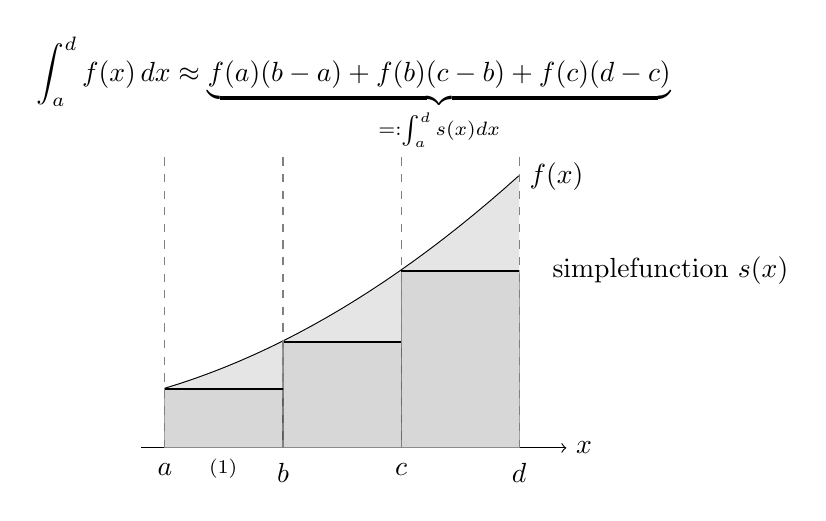
\begin{tikzpicture}[scale=1.5]
  % Achsen
  \draw[->] (-0.2,0) -- (3.4,0) node[right] {$x$};
  % Kontinuierliche Funktion f(x)
  \draw[thick,domain=0:3,smooth] plot(\x,{0.5+0.3*\x+0.1*\x*\x}) node[right] {$f(x)$};
  % Fläche unter f(x) schattieren
  \fill[gray!20] (0,0) -- plot[domain=0:3] (\x,{0.5+0.3*\x+0.1*\x*\x}) -- (3,0) -- cycle;
  % Treppenfunktion: linke Endpunkte der Intervalle [0,1], [1,2], [2,3]
  \draw[fill=gray!50,opacity=0.35] (0,0) rectangle (1,0.5);
  \node at (0.5,-0.2) {$\cluster^{(1)}$}; 
  \draw[fill=gray!50,opacity=0.35] (1,0) rectangle (2,0.9);
  \draw[fill=gray!50,opacity=0.35] (2,0) rectangle (3,1.5);
  % Linien der Treppenfunktion
  \draw[thick] (0,0.5)--(1,0.5);
  \draw[thick] (1,0.9)--(2,0.9);
  \draw[thick] (2,1.5)--(3,1.5);
  % Gepunktete Linien der Partition
  \foreach \x in {0,1,2,3} \draw[dashed,gray] (\x,0) -- (\x,2.5);
  % Beschriftungen
  \node[anchor=north] at (0,-0.05) {$a$};
  \node[anchor=north] at (1,-0.05) {$b$};
  \node[anchor=north] at (2,-0.05) {$c$};
  \node[anchor=north] at (3,-0.05) {$d$};
  \node at (1.6,3.0) {$\displaystyle \int_a^d f(x)\,dx \approx \underbrace{f(a)(b-a) + f(b)(c-b)+f(c)(d-c)}_{=:\int_a^d s(x)dx}$};
  \node [anchor=west] at (3.2,1.5) {\gls{simplefunction} $s(x)$};
\end{tikzpicture}
\end{figure}
Es ist nützlich, das Lebesgue-Integral als \gls{function} zu betrachten, die jede integrierbare 
\gls{function} $f$ auf den Wert ihres Integrals abbildet:
$$ f \mapsto \int_{\featurevec} f(\featurevec) d\featurevec.$$ 
Die präzise Definition dieser \gls{function}, einschließlich ihres \gls{domain}, 
welches die integrierbaren \glspl{function} umfasst, ist ein Grundpfeiler der 
Maßtheorie \cite[Ch. 1]{RudinBook}.
					\\ 
		Siehe auch: \gls{function}.},
	first={Lebesgue-Integral},
	type=math, 
	firstplural={Lebesgue-Integrale}
}

\newglossaryentry{cdf}
{name={kumulative Verteilungsfunktion (cdf)},
	description={Die \index{kumulative Verteilungsfunktion (cdf)} cdf 
	$\cdf{\feature}{\eta}$ einer reellen \gls{rv} $\feature$ ist definiert als \cite{AshProbMeasure,papoulis}
	$$\cdf{\feature}{\eta} \defeq \prob{\feature \leq \eta}.$$
					\\ 
		Siehe auch: \gls{pdf}, \gls{probdist}, \gls{rv}.},
	first={kumulative Verteilungsfunktion (cdf)},
	firstplural={kumulative Verteilungsfunktionen (cdfs)}, 
	plural={cdfs}, 
	type=math,
	text={cdf} 
}

\newglossaryentry{weightedgraph}
{name={gewichteter Graph},
	description={Ein \gls{graph}\index{gewichteter Graph}, dessen Kanten numerische Gewichte 
	erhalten. Typischerweise sind diese Kantengewichte nichtnegative reelle Zahlen. 
	Beispielsweise kann in einem Graphen, der ein Straßennetz darstellt, wobei die Knoten Kreuzungen 
	sind und die Kanten Straßenabschnitte darstellen, das Kantengewicht die Kapazität 
	(maximale Fahrzeuge pro Stunde) des Straßenabschnitts darstellen \cite{NewmannBook}.  
					\\ 
		Siehe auch: \gls{graph}.},
	first={gewichteter Graph},
	type=math,
	firstplural={gewichtete Graphen}, 
	plural={gewichtete Graphen}, 
	text={gewichteter Graph} 
}


\newglossaryentry{graph}
{
	name={Graph},
	description={Ein \index{Graph} Graph $\graph = \pair{\nodes}{\edges}$ ist ein Paar, bestehend aus 
		einer Knotenmenge $\nodes$ und einer Kantenmenge $\edges$. In der allgemeinsten Form wird ein Graph durch eine Abbildung beschrieben, 
		die jeder Kante $\edgeidx \in \edges$ ein Paar von Knoten zuordnet \cite{RockNetworks}. 
		Eine wichtige Familie von Graphen sind einfache ungerichtete Graphen. Ein einfacher ungerichteter Graph entsteht durch Identifikation 
		jeder Kante $\edgeidx \in \edges$ mit zwei verschiedenen Knoten $\{\nodeidx, \nodeidx'\}$. 
		Gewichtete Graphen spezifizieren zusätzlich numerische \gls{weights} $\edgeweight_{\edgeidx}$ für jede Kante $\edgeidx \in \edges$.},
	first={Graph}, text={Graph}, plural={Graphen}
}


\newglossaryentry{uncertainty}
{
	name={Unsicherheit},
	description={Unsicherheit\index{Unsicherheit} bezeichnet den Grad des Vertrauens — oder das Fehlen desselben — 
		in eine Größe wie eine \gls{model} \gls{prediction}, eine Parameterschätzung oder eine beobachtete \gls{datapoint}. 
		Im \gls{ml} entsteht Unsicherheit aus verschiedenen Quellen, darunter verrauschte \gls{data}, begrenzte Trainingsstichproben 
		oder Mehrdeutigkeit in den \gls{model}-Annahmen. Die \gls{probability}-Theorie bietet einen prinzipiellen Rahmen, 
		um solche Unsicherheiten zu modellieren und zu quantifizieren.},
	first={Unsicherheit}, text={Unsicherheit}
}

\newglossaryentry{ucb}
{
	name={obere Konfidenzgrenze (Upper Confidence Bound, UCB)},
	description={Betrachte eine \index{obere Konfidenzgrenze (UCB)} \gls{ml}-Anwendung, 
		die in jedem Zeitschritt $\iteridx$ eine Aktion $\action_{\iteridx}$ aus einer endlichen Menge 
		alternativer Aktionen $\actionset$ auswählt. Der Nutzen der Auswahl von Aktion 
		$\action_{\iteridx}$ wird durch ein numerisches \gls{reward}-Signal $\reward^{(\action_{\iteridx})}$ quantifiziert. 
		
		Ein weit verbreitetes \gls{probmodel} für dieses sequentielle Entscheidungsproblem 
		ist das stochastische Multi-Armed-Bandit-(MAB-)Modell \cite{Bubeck2012}. In diesem \gls{model} 
		wird der \gls{reward} $\reward^{(\action)}$ als Realisierung einer \gls{rv} mit unbekanntem 
		\gls{mean} $\mu^{(\action)}$ betrachtet. Idealerweise wählt man stets die Aktion mit dem 
		grössten erwarteten \gls{reward} $\mu^{(\action)}$, doch diese \gls{mean}s sind unbekannt 
		und müssen aus beobachteten \gls{data} geschätzt werden. Eine einfache Strategie, immer die Aktion 
		mit dem höchsten Schätzwert $\widehat{\mu}^{(\action)}$ zu wählen, kann wegen der 
		Schätzunsicherheit zu suboptimalen Ergebnissen führen. 
		
		Die UCB-Strategie adressiert dieses Problem, indem sie Aktionen nicht nur nach ihren geschätzten 
		\gls{mean}s auswählt, sondern auch einen Term berücksichtigt, der die Unsicherheit dieser 
		Schätzungen widerspiegelt — sie bevorzugt somit Aktionen mit hohem potenziellem \gls{reward} 
		und hoher Unsicherheit. Theoretische Garantien für die Performance von UCB-Strategien, 
		insbesondere logarithmische \gls{regret}-Schranken, finden sich in \cite{Bubeck2012}.},
	first={obere Konfidenzgrenze (UCB)}, text={UCB}
}

\newglossaryentry{mab}
{
	name={Multi-Armed Bandit (MAB)},
	description={Ein Multi-Armed Bandit (MAB)\index{Multi-Armed Bandit (MAB)}-Problem modelliert ein wiederholtes Entscheidungsproblem, 
		bei dem in jedem Zeitschritt $\iteridx$ ein Lernender eine von mehreren möglichen Aktionen, oft als „Arme“ bezeichnet, aus einer endlichen Menge 
		$\actionset$ auswählen muss. Jeder Arm $\action \in \actionset$ liefert eine stochastische \gls{reward} $\reward^{(\action)}$, 
		die aus einer unbekannten \gls{probdist} mit Erwartungswert $\mu^{(\action)}$ gezogen wird. 
		
		Ziel des Lernenden ist es, die kumulative \gls{reward} über die Zeit zu maximieren, indem er geschickt die Balance zwischen Exploration 
		(d.h. dem Sammeln von Informationen über unsichere Arme) und Exploitation (d.h. der Auswahl von Armen, die bekanntlich gut performen) hält. 
		
		Diese Balance wird durch das Konzept des \gls{regret} quantifiziert, das die Leistungsdifferenz zwischen der Strategie des Lernenden und der optimalen Strategie misst, 
		die stets den besten Arm auswählt. MAB-Probleme bilden ein fundamentales \gls{model} im Online-Lernen, Reinforcement Learning und sequentiellen Experimentdesign \cite{Bubeck2012}.},
	first={Multi-Armed Bandit (MAB)}, text={MAB}
}

\newglossaryentry{optimism_in_face_of_uncertainty}
{name={Optimismus im Angesicht der Unsicherheit},
	description={
		\index{Optimismus im Angesicht der Unsicherheit}
		ML-Methoden verwenden ein Leistungsmaß $\bar{f}(\weights)$ um Modell-Parameter $\weights$ 
		zu lernen. Allerdings haben sie in der Regel keinen direkten Zugriff auf $\bar{f}(\weights)$, 
		sondern nur auf eine Schätzung (oder Annäherung) $f(\weights)$. Zum Beispiel verwenden herkömmliche 
		ML Methoden einen Trainingsfehler als Schätzung für den erwarteten Verlust. 
		Mit einem probabilistischen Modell lässt sich ein Konfidenzintervall $\big[ l^{(\weights)},  u^{(\weights)} \big]$ für jede Wahl von Modellparametern konstruieren. 
		Eine einfache Konstruktion hierfür ist $l^{(\weights)} \defeq f(\weights) - \sigma/2$, $u^{(\weights)} \defeq f(\weights) + \sigma/2$, 
		wobei $\sigma$ ein Maß für die (erwartete) Abweichung von $f(\weights)$ zu $\bar{f}(\weights)$ ist. 
		Es können auch andere Konstruktionen für dieses Intervall verwendet werden, solange sie sicherstellen, 
		dass mit ausreichend hoher Wahrscheinlichkeit $\bar{f}(\weights) \in \big[ l^{(\weights)},  u^{(\weights)} \big]$ gilt. 
		Als Optimist wählen wir $\weights$ gemäß dem günstigsten – aber dennoch plausiblen – Wert 
		$\tilde{f}(\weights) \defeq l^{(\weights)}$ des Leistungsmaßes. Zwei Beispiele für diese Konstruktion 
	    findet man in der strukturellen Risikominimierung \cite[Kap. 11]{ShalevMLBook} sowie bei Methoden für 
	    die sequentielle Entscheidungsfindung 
	    \cite[Abschnitt 2.2]{Bubeck2012}. 
		\begin{figure}[htbp]
			\begin{center}
				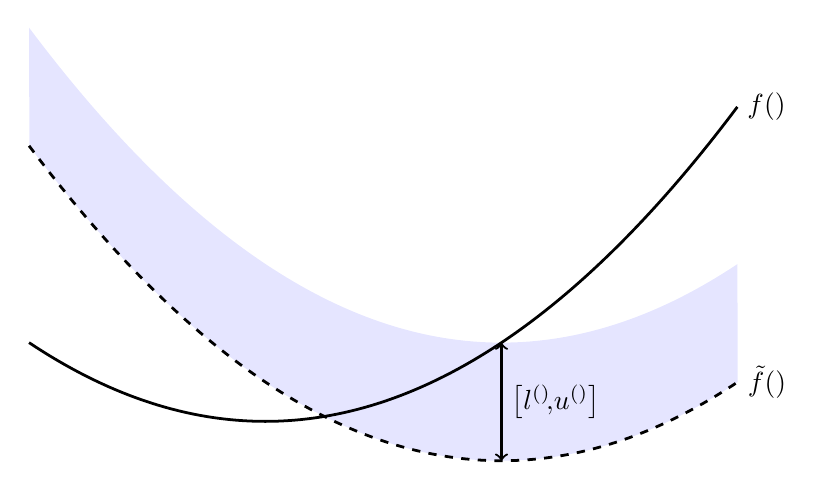
\begin{tikzpicture}[x=3cm, y=1cm]
					% Filled band around the quadratic curve with different boundary curves
					\fill[blue!10] 
					(-1, 5) -- plot[domain=-2:1, samples=100] ({\x+1}, {\x*\x + 1}) -- 
					plot[domain=1:-2, samples=100] ({\x+1}, {\x*\x - 0.5}) -- cycle;
					\node[anchor=west] at (2, 4) {$f(\weights)$};
					\draw[line width=1, domain=-2:1, samples=100,dashed] plot  ({\x+1}, {\x*\x -0.5}) node[right] {$\tilde{f}(\weights)$};
					\draw[line width=1, domain=-1:2, samples=100] plot ({\x}, {\x*\x});
					\draw[<->, thick] (1, -0.5) -- (1, 1) node[midway, right] {$\big[ l^{(\weights)}\!,\!u^{(\weights)} \big]$};
				\end{tikzpicture}
				\caption{Wir verwenden eine Schätzung $f(\weights)$ für das Leistungsmaß $\bar{f}(\weights)$ 
					um ein Konfidenzintervall $\big[ l^{(\weights)},  u^{(\weights)} \big]$ zu konstruieren. Ein Optimist 
					im Angesicht der Unsicherheit wählt Modellparameter $\weights$ gemäß dem günstigsten –
					 aber dennoch plausiblen – Wert $\tilde{f}(\weights) \defeq l^{(\weights)}$.} 
			\end{center}
	\end{figure}},first={Optimismus im Angesicht der Unsicherheit},text={Optimismus im Angesicht der Unsicherheit} 

\newglossaryentry{empgraph}
{
	name={Föderiertes Lernen Netzwerk (FL network)},
	description={Ein \gls{fl}-Netzwerk\index{federated learning network (FL network)} ist ein ungerichteter, 
	gewichteter \gls{graph}, dessen Knoten \gls{data}-Erzeuger repräsentieren, die lokale 
	(oder personalisierte) \gls{modelle} trainieren möchten. Jeder Knoten in einem \gls{fl}-Netzwerk steht 
	für ein \gls{device}, das in der Lage ist, ein \gls{localdataset} zu sammeln und daraus ein \gls{localmodel}
	 zu trainieren. \Gls{fl}-Methoden lernen für jeden Knoten $\nodeidx \in \nodes$ eine lokale \gls{hypothesis} $\localhypothesis{\nodeidx}$, 
	 sodass die \gls{loss} auf den jeweiligen \gls{localdataset}s minimiert wird.},
	first={föderiertes Lernen Netzwerk (FL network)},text={FL network} 
}


\newglossaryentry{norm}
{
	name={Norm},
	description={Eine \index{Norm} Norm ist eine Abbildung, die jedem (Vektor-)Element eines linearen Vektorraums 
	eine nicht-negative reelle Zahl zuordnet. Diese Abbildung muss homogen und definit sein sowie die Dreiecksungleichung 
	erfüllen \cite{HornMatAnalysis}.},
	first={Norm},text={Norm} 
}


\newglossaryentry{dualnorm}
{
	name={duale Norm},
	description={Jede \gls{norm} $\normgeneric{\cdot}{}$, definiert auf einem \gls{euclidspace} $\mathbb{R}^{\dimlocalmodel}$, besitzt eine zugehörige duale \gls{norm}, bezeichnet mit $\normgeneric{\cdot}{*}$ und definiert durch
		\[
		\normgeneric{\vy}{*} \defeq \sup_{\norm{\vx}{} \leq 1} \vy^{T} \vx.
		\]
		Die duale \gls{norm} misst das maximal mögliche Skalarprodukt zwischen $\vy$ und einem Vektor aus der Einheitskugel der ursprünglichen \gls{norm}. Weitere Details finden sich in \cite[Abschnitt A.1.6]{BoydConvexBook}.},
	first={duale Norm},
	text={duale Norm}
}

\newglossaryentry{geometricmedian}{
	name={geometrische Mitte (GM)},
	description={Die GM\index{geometrische Mitte (GM)} einer Menge von Eingabevektoren $\vx^{(1)}, \ldots, \vx^{(\samplesize)}$ 
		in $\mathbb{R}^{\dimlocalmodel}$ ist ein Punkt $\vz \in \mathbb{R}^{\dimlocalmodel}$, der 
		die Summe der Abstände zu diesen Vektoren minimiert \cite{BoydConvexBook}, d.\,h. 
		\begin{equation} 
			\label{equ_geometric_median}
			\vz \in \argmin_{\vy \in \mathbb{R}^{\dimlocalmodel}} \sum_{\sampleidx=1}^{\samplesize} \normgeneric{\vy - \vx^{(\sampleidx)}}{2}.
		\end{equation} 
		\begin{figure}[H]
			\begin{center}
				\begin{tikzpicture}[scale=2, thick, >=stealth]
					\coordinate (w) at (3,0);
					\fill (w) circle (1.2pt) node[below right] {$\vz$};
					\coordinate (w2) at (0.5,0.3);
					\coordinate (w3) at (0.7,0.7);
					\fill (w2) circle (1pt) node[above left] {$\vx^{(1)}$};
					\fill (w3) circle (1pt) node[above left] {$\vx^{(2)}$};
					\draw[dashed] (w) -- (w2);
					\draw[dashed] (w) -- (w3);
					\draw[->, thick, red] (w) -- ($(w)!1cm!(w2)$) ;
					\draw[->, thick, red] (w) -- ($(w)!1cm!(w3)$) node[pos=0.9, right,yshift=7pt] {$\frac{\vx^{(2)}- \vz}{\normgeneric{\vx^{(2)}-\vz}{2}}$};
					\coordinate (w4) at (5,0.2);
					\node at (5,0.4) {\textbf{Gestört}};
					\fill (w4) circle (1pt) node[below left] {$\vx^{(3)}$};
					\draw[->, thick, red] (w) -- ($(w)!1cm!(w4)$) ;
				\end{tikzpicture}
				\caption{\label{opt_cond_GM}
					Betrachte eine Lösung $\vz$ von \eqref{equ_geometric_median}, die nicht mit einem der Eingabevektoren übereinstimmt. 
					Die Optimalitätsbedingung für \eqref{equ_geometric_median} verlangt, dass die Einheitsvektoren von $\vz$ zu den Eingabevektoren 
					in der Summe null ergeben.}
			\end{center}
		\end{figure}
		Abbildung~\ref{opt_cond_GM} illustriert eine fundamentale Eigenschaft der GM:
		Falls $\vz$ nicht mit einem der Eingabevektoren übereinstimmt, müssen die Einheitsvektoren, 
		die von $\vz$ zu jedem $\vx^{(\sampleidx)}$ zeigen, in der Summe null ergeben — dies ist die 
		Null-\gls{subgradient}- (Optimalitäts-) Bedingung von \eqref{equ_geometric_median}. 
		Es zeigt sich, dass die Lösung von \eqref{equ_geometric_median} nicht beliebig weit von den vertrauenswürdigen 
		Eingabevektoren weggezogen werden kann, solange diese die Mehrheit bilden \cite[Th. 2.2]{Lopuhaae1991}.},
	first={geometrische Mitte},
	text={GM}
}

\newglossaryentry{explanation}
{name={Erklärung},
	description={Ein Ansatz, um \gls{ml}-Methoden transparenter zu machen, besteht darin, 
		eine Erklärung\index{Erklärung} zusammen mit der von einer \gls{ml}-Methode gelieferten 
		\gls{prediction} bereitzustellen. Erklärungen können in unterschiedlichen Formen auftreten. 
		Eine Erklärung kann beispielsweise ein natürlichsprachlicher Text sein oder eine quantitative 
		Maßzahl, welche die Bedeutung einzelner \gls{feature}s eines \gls{datapoint}s beschreibt \cite{Molnar2019}. 
		Es können auch visuelle Formen von Erklärungen genutzt werden, etwa Intensitätskarten bei der Bild-\gls{classification} \cite{GradCamPaper}.},
	first={Erklärung},text={Erklärung} 
}

\newglossaryentry{risk}
{name={Risiko},
	description={Betrachte\index{Risiko} eine \gls{hypothesis} $\hypothesis$, die verwendet wird, um das \gls{label} 
		$\truelabel$ eines \gls{datapoint} auf Basis seiner \gls{feature}s $\featurevec$ vorherzusagen. 
		Die Qualität einer bestimmten \gls{prediction} wird mithilfe einer \gls{lossfunc} 
		$\lossfunc{(\featurevec,\truelabel)}{\hypothesis}$ gemessen. Wenn wir \gls{datapoint}s als 
		\gls{realization}en von \glspl{rv} interpretieren, die \gls{iid} sind, dann wird auch 
		$\lossfunc{(\featurevec,\truelabel)}{\hypothesis}$ zur \gls{realization} einer \gls{rv}. 
		Die Annahme der \gls{iidasspt} erlaubt es uns, das Risiko einer \gls{hypothesis} als den erwarteten 
		\gls{loss} zu definieren: $\expect \big\{\lossfunc{(\featurevec,\truelabel)}{\hypothesis} \big\}$. 
		Beachte, dass das Risiko von $\hypothesis$ sowohl von der konkreten Wahl der \gls{lossfunc} 
		als auch von der \gls{probdist} der \gls{datapoint}s abhängt.},
	first={Risiko},text={Risiko}, plural={Risiken}
}

\newglossaryentry{actfun}
{name={Aktivierungsfunktion},
	description={Jedem\index{Aktivierungsfunktion} künstlichen Neuron innerhalb eines \gls{ann} 
		wird eine Aktivierungsfunktion $\actfun(\cdot)$ zugewiesen, die eine gewichtete 
		Kombination der Neuronen-Eingaben $\feature_{1},\ldots,\feature_{\nrfeatures}$ 
		auf einen einzelnen Ausgabewert abbildet: 
		$a = \actfun\big(\weight_{1} \feature_{1}+\ldots+\weight_{\nrfeatures} \feature_{\nrfeatures} \big)$. 
		Jedes Neuron ist dabei durch die \glspl{weights} $\weight_{1},\ldots,\weight_{\nrfeatures}$ parametrisiert.},
	first={Aktivierungsfunktion},text={Aktivierungsfunktion} , plural={Aktivierungsfunktionen}
}

\newglossaryentry{distributedalgorithm}
{name={verteiltes Algorithmusverfahren},
	description={Ein\index{verteiltes Algorithmusverfahren} verteiltes \gls{algorithmus}verfahren ist ein \gls{algorithmus}, 
		der für eine spezielle Art von Rechensystemen entwickelt wurde, nämlich für eine Sammlung 
		interagierender Rechengeräte (sogenannte Knoten). Diese Knoten kommunizieren und koordinieren 
		ihre lokalen Berechnungen durch den Austausch von Nachrichten über ein Netzwerk 
		\cite{IntroDistAlg}, \cite{ParallelDistrBook}. Im Gegensatz zu einem klassischen \gls{algorithmus}, 
		der auf einem einzelnen \gls{device} ausgeführt wird, läuft ein verteiltes \gls{algorithmus}verfahren 
		gleichzeitig auf mehreren \gls{device}s mit eigener Rechenkapazität ab. 
		
		Ähnlich wie ein klassischer \gls{algorithmus} lässt sich auch ein verteiltes Verfahren als 
		Menge möglicher Ausführungsverläufe modellieren. Allerdings beinhalten die Ausführungen im 
		verteilten Fall sowohl lokale Berechnungen als auch Kommunikationsereignisse. 
		Eine typische Ausführung könnte folgendermaßen aussehen:
		\[
		\begin{array}{l}
			\text{Knoten 1: } {\rm input}_1, s_1^{(1)}, s_2^{(1)}, \ldots, s_{T_1}^{(1)}, {\rm output}_1; \\
			\text{Knoten 2: } {\rm input}_2, s_1^{(2)}, s_2^{(2)}, \ldots, s_{T_2}^{(2)}, {\rm output}_2; \\
			\quad \vdots \\
			\text{Knoten N: } {\rm input}_N, s_1^{(N)}, s_2^{(N)}, \ldots, s_{T_N}^{(N)}, {\rm output}_N.
		\end{array}
		\]
		Jedes \gls{device} $\nodeidx$ beginnt mit einem eigenen lokalen Eingabewert und führt eine Sequenz 
		von Zwischenrechnungen $s_{\iteridx}^{(\nodeidx)}$ zu diskreten Zeitpunkten $\iteridx = 1, \dots, T_\nodeidx$ durch. 
		Diese Berechnungen können sowohl von vorherigen lokalen Berechnungsschritten als auch von empfangenen 
		Nachrichten anderer \gls{device}s abhängen. 
		
		Eine wichtige Anwendung verteilter \glspl{algorithmus} ist das \gls{fl}, bei dem ein Netzwerk 
		von \glspl{device} kollaborativ ein persönliches \gls{model} für jedes \gls{device} trainiert.},
	first={verteiltes Algorithmusverfahren}, text={verteiltes Algorithmusverfahren}
}

\newglossaryentry{algorithm}
{name={Algorithmus},
	description={Ein\index{Algorithmus} Algorithmus ist eine präzise, schrittweise Vorschrift, 
		wie aus einer gegebenen Eingabe in endlich vielen Rechenschritten eine Ausgabe erzeugt wird \cite{Cormen:2022aa}. 
		Ein Beispiel ist ein Algorithmus zum Trainieren eines \gls{linmodel}, der explizit beschreibt, 
		wie ein gegebenes \gls{trainset} durch eine Folge von \glspl{gradstep} in \glspl{modelparams} 
		transformiert wird. 
		
		Diese informelle Beschreibung lässt sich durch verschiedene mathematische \gls{model}le 
		rigide formalisieren \cite{Sipser2013}. Ein einfaches \gls{model} eines Algorithmus ist 
		die Menge möglicher Ausführungen, wobei jede Ausführung eine Folge der Form
		$${\rm input},s_1,s_2,\ldots,s_T,{\rm output}$$
		darstellt, die den Beschränkungen der zugrunde liegenden Rechenarchitektur genügt.
		
		Algorithmen können \emph{deterministisch} sein, sodass jede Eingabe zu einer eindeutig bestimmten 
		Ausführung führt, oder \emph{randomisiert}, wobei sich Ausführungen mit gewisser Wahrscheinlichkeit 
		unterscheiden. Randomisierte Algorithmen lassen sich daher durch stochastische Prozesse analysieren, 
		wobei Ausführungsfolgen als Ergebnisse zufälliger Experimente modelliert werden 
		\cite{BertsekasProb}, \cite{RandomizedAlgos}, \cite{Gallager13}.
		
		Wesentlich ist, dass ein Algorithmus mehr umfasst als lediglich eine Abbildung von Eingabe 
		auf Ausgabe: Auch die Zwischenschritte $s_1,\ldots,s_T$ gehören zur vollständigen Beschreibung des Verfahrens.},
	first={Algorithmus},text={Algorithmus}, plural={Algorithmen}
}

\newglossaryentry{stochalgorithm}
{name={stochastischer Algorithmus}, 
 plural={stochastische Algorithmen},
	description={Ein\index{stochastischer Algorithmus} \gls{stochastischer} \gls{Algorithmus} nutzt während seiner Ausführung einen Zufallsmechanismus. 
		Beispielsweise verwendet \gls{stochGD} eine zufällig ausgewählte Teilmenge von \glspl{datapoint}, 
		um eine Näherung für den \gls{gradient} einer \gls{objfunc} zu berechnen. 
		Wir können einen \gls{stochastischen} \gls{Algorithmus} durch einen \glspl{stochproc} darstellen, 
		d. h., die möglichen Ausführungsfolgen entsprechen den möglichen Ergebnissen eines 
		\gls{randomexperiment} \cite{BertsekasProb}, \cite{RandomizedAlgos}, \cite{Gallager13}.		
		\\ 
		Siehe auch: \gls{stochastic}, \gls{algorithm}, \gls{stochGD}, \gls{datapoint}, \gls{gradient}, \gls{objfunc}, \gls{stochproc}, 
		\gls{randomexperiment}, \gls{optmethod}, \gls{gdmethod}. },
	first={stochastischer Algorithmus},
	text={stochastischer Algorithmus} 
}

\newglossaryentry{batchlearning}
{name={Batch-Lernen},
	description={Beim \gls{batch} Lernen\index{Batch-Lernen} (auch als Offline-Lernen bekannt) wird das \gls{ml} \gls{model} 
		auf dem gesamten \gls{dataset} in einer einzigen Trainingsiteration trainiert, anstatt es inkrementell zu aktualisieren, sobald neue \gls{data} eintreffen. 
		Alle verfügbaren \gls{data} werden in einen Lern-\gls{algorithm} eingespeist, wodurch ein \gls{model} entsteht, das \glspl{prediction} liefern kann. 
		Da diese \glspl{dataset} oft groß sind, ist das Training rechenaufwendig und zeitintensiv und wird daher typischerweise offline durchgeführt. 
		Nach dem Lernen ist das \gls{model} statisch und passt sich nicht automatisch an neue \gls{data} an. 
		Ein Aktualisieren des \gls{model} mit neuen Informationen erfordert ein vollständiges Retraining. 
		Sobald das \gls{model} trainiert ist, wird es in die Produktion gebracht, wo es nicht aktualisiert werden kann. 
		Da das Training eines \gls{model} viele Stunden dauern kann, werden viele \glspl{model} in Produktionsumgebungen zyklisch nach einem festen Zeitplan aktualisiert, 
		wenn die \gls{data}-Verteilung stabil ist. Beispielsweise könnte ein Einzelhandels-Analytics-Team ihr Nachfrageprognose-\gls{model} jeden Sonntag 
		mit den Verkaufsdaten der Vorwoche neu trainieren, um die Nachfrage der nächsten Woche vorherzusagen. 
		Falls ein System kontinuierlich an schnell ändernde \gls{data} angepasst werden muss, wie z. B. bei der Vorhersage von Aktienkursen, 
		ist eine anpassungsfähigere Lösung wie \gls{onlinelearning} erforderlich.
		\\
		Siehe auch: \gls{batch}, \gls{model}, \gls{dataset}, \gls{onlinelearning}. },
	first={Batch-Lernen}, 
	text={Batch-Lernen}
}

\newglossaryentry{onlinelearning}
{name={Online-Lernen},
	description={Einige \gls{ml}-Methoden\index{Online-Lernen} sind darauf ausgelegt, \gls{data} 
		sequentiell zu verarbeiten und ihre \glspl{modelparam} jeweils einzeln zu aktualisieren, sobald neue \glspl{datapoint} verfügbar werden. 
		Ein typisches Beispiel sind Zeitreihen-\gls{data}, wie tägliche \gls{minimum}- und \gls{maximum}-Temperaturen, 
		die von einer \gls{fmi}-Wetterstation aufgezeichnet werden. Diese Werte bilden eine chronologische Folge von Beobachtungen. 
		In jedem Zeitschritt $\timeidx$ aktualisieren (oder verfeinern) Online-Lernmethoden die aktuelle \gls{hypothesis} 
		$\hypothesis^{(\timeidx)}$ (oder \glspl{modelparam} $\weights^{(\timeidx)}$) basierend auf dem neu beobachteten \gls{datapoint} 
		$\datapoint^{(\timeidx)}$.
		\\ 
		Siehe auch: \gls{onlineGD}, \gls{onlinealgorithm}. },
	first={Online-Lernen},
	text={Online-Lernen}
}


\newglossaryentry{onlinealgorithm}
{name={Online-Algorithmus},
	description={Ein\index{Online-Algorithmus} Online-\gls{algorithmus} verarbeitet Eingabedaten inkrementell, 
		indem die \gls{data} schrittweise empfangen und unmittelbar verarbeitet werden, 
		d.h. Entscheidungen oder Ausgaben erfolgen sofort, ohne dass der gesamte Eingabestrom im Voraus bekannt ist 
		\cite{PredictionLearningGames}, \cite{HazanOCO}. 
		
		Im Gegensatz zu einem Offline-\gls{algorithmus}, der von Anfang an Zugriff auf die vollständige Eingabe hat, 
		muss ein Online-\gls{algorithmus} mit der \gls{uncertainty} zukünftiger Eingaben umgehen und kann frühere 
		Entscheidungen nicht revidieren. Ähnlich wie ein Offline-\gls{algorithmus} lässt sich ein Online-\gls{algorithmus} 
		formal als Menge möglicher Ausführungsverläufe modellieren. Die Struktur einer Ausführung unterscheidet sich jedoch 
		grundlegend und folgt dem Schema:
		\[
		{\rm in}_{1},s_1,{\rm out}_{1},{\rm in}_{2},s_2,{\rm out}_{2},\ldots,{\rm in}_{T},s_T,{\rm out}_{T}.
		\]
		Jede Ausführung beginnt mit einem initialen Zustand (\({\rm in}_{1}\)) und besteht aus abwechselnden 
		Rechenschritten, Ausgaben (oder Entscheidungen) und neu eingehenden Daten. 
		Im Schritt \(\iteridx\) führt der \gls{algorithmus} eine Berechnung \(s_{\iteridx}\) aus, 
		erzeugt eine Ausgabe \({\rm out}_{\iteridx}\) und erhält anschließend die nächste Eingabe \({\rm in}_{\iteridx+1}\). 
		
		Ein bekanntes Beispiel für einen Online-\gls{algorithmus} im Bereich \gls{ml} ist der 
		\gls{onlineGD}, bei dem \glspl{modelparams} schrittweise aktualisiert werden, sobald neue 
		\glspl{datapoint} eintreffen.},
	first={Online-Algorithmus},text={Online-Algorithmus} 
}

\newglossaryentry{transparency}
{name={Transparenz},
	description={Transparenz\index{Transparenz} ist eine grundlegende Voraussetzung für 
		\gls{trustAI} \cite{HLEGTrustworhtyAI}. Im Kontext von \gls{ml}-Methoden wird Transparenz 
		oft synonym mit \gls{explainability} verwendet \cite{JunXML2020}, \cite{gallese2023ai}. 
		Im weiteren Sinne von \gls{ai}-Systemen umfasst Transparenz jedoch mehr als nur 
		Erklärbarkeit: Sie beinhaltet auch die Offenlegung von Beschränkungen, Zuverlässigkeit 
		und dem beabsichtigten Einsatzgebiet des Systems. 
		
		In medizinischen Diagnosesystemen bedeutet Transparenz etwa die Angabe der Vertrauenswürdigkeit 
		der vom trainierten \gls{model} gelieferten \gls{prediction}en. Im Bereich der Kreditvergabe 
		sollten \gls{ai}-basierte Entscheidungen durch Erklärungen der relevanten Einflussfaktoren 
		– etwa Einkommen oder Kreditgeschichte – begleitet werden. Diese Erklärungen ermöglichen es 
		den Betroffenen, etwa Kreditnehmern, die automatisierten Entscheidungen nachzuvollziehen und anzufechten. 
		
		Einige \gls{ml}-Methoden bieten von Natur aus Transparenz: So liefert \gls{logreg} 
		eine quantitative Abschätzung der Zuverlässigkeit einer \gls{classification} über den Wert $|\hypothesis(\featurevec)|$. 
		\Gls{decisiontree}s sind ein weiteres Beispiel, da sie gut verständliche Entscheidungsregeln 
		bieten \cite{rudin2019stop}.
		
		Transparenz verlangt zudem eine klare Kennzeichnung, wenn ein Benutzer mit einem \gls{ai}-System interagiert. 
		Beispielsweise sollten \gls{ai}-gestützte Chatbots ihre Nutzer darüber informieren, dass sie mit einem automatisierten 
		System und nicht mit einem Menschen kommunizieren. 
		
		Darüber hinaus umfasst Transparenz eine umfassende Dokumentation, welche Zweck, Designentscheidungen 
		und vorgesehenen Einsatzbereiche des \gls{ai}-Systems erläutert. Beispielhaft sind hier 
		\gls{model}-Datasheets \cite{DatasheetData2021} und \gls{ai}-System-Cards \cite{10.1145/3287560.3287596}, 
		die Praktiker:innen helfen, die Einsatzmöglichkeiten und Grenzen eines \gls{ai}-Systems zu verstehen \cite{Shahriari2017}.},
	first={Transparenz}, text={Transparenz} 
}

\newglossaryentry{sensattr}
{
	name={sensitive Attribut},
	description={
		\gls{ml}\index{sensitive Attribut} bezeichnet das Gebiet des maschinellen Lernens, bei dem 
		eine \gls{hypothesis}-Funktion erlernt wird, die es ermöglicht, das \gls{Label} eines \gls{Datenpunkts} 
		anhand seiner \glspl{feature} vorherzusagen. In bestimmten Anwendungsfällen muss sichergestellt werden, 
		dass die Ausgabe eines \gls{ML}-Modells keine Rückschlüsse auf sensitive Attribute eines \gls{Datenpunkts} zulässt. Welche Merkmale eines \gls{Datenpunkts} als sensitive Attribute klassifiziert werden, ist eine kontextspezifische Designentscheidung und variiert je nach Anwendungsgebiet.
	},
	first={sensitives Attribut},
	text={sensitives Attribut}, plural={sensitive Attribute}
}


\newglossaryentry{sbm}
{
	name={stochastisches Blockmodell (SBM)},
	description={
		Das\index{stochastisches Blockmodell (SBM)} stochastische Block-\gls{modell} ist ein probabilistisches generatives \gls{modell} für einen ungerichteten \gls{graph} $\graph = \big( \nodes, \edges \big)$ 
		mit einer gegebenen Menge von Knoten $\nodes$ \cite{AbbeSBM2018}. In seiner einfachsten Variante 
		generiert das stochastische Block-\gls{modell} einen \gls{graph}, indem zunächst jeder Knoten $\nodeidx \in \nodes$ 
		zufällig einem \gls{cluster}-Index $\clusteridx_{\nodeidx} \in \{1,\ldots,\nrcluster\}$ zugeordnet wird. 
		Ein Paar verschiedener Knoten im \gls{graph} wird mit einer \gls{wahrscheinlichkeit} $p_{\nodeidx,\nodeidx'}$ verbunden, 
		die ausschließlich von den \gls{label}n $\clusteridx_{\nodeidx}, \clusteridx_{\nodeidx'}$ abhängt. 
		Das Vorhandensein von Kanten zwischen verschiedenen Knotenpaaren ist statistisch unabhängig.
	},
	first={stochastisches Blockmodell (SBM)},
	text={SBM}, 
	plural={stochastische Blockmodelle (SBMs)}
}

\newglossaryentry{deepnet}
{
	name={Deep Net},
	description={
		Ein\index{Deep Net} Deep Net ist ein \gls{ANN} mit einer (relativ) großen Anzahl von 
		versteckten Schichten. Deep Learning ist ein Oberbegriff für \gls{ML}-Methoden, die ein Deep
		 Net als ihr \gls{Modell} verwenden \cite{Goodfellow-et-al-2016}.
	},
	first={Deep Net},
	text={Deep Net}
}


\newglossaryentry{baseline}
{
	name={Baseline},
	description={
		Betrachte\index{Baseline} eine \gls{ML}-Methode, die eine gelernte \gls{Hypothese} (bzw. ein trainiertes \gls{Modell}) $\learnthypothesis \in \hypospace$ liefert.
		 Die Qualität eines trainierten \gls{model}s wird häufig über den durchschnittlichen \gls{Loss} auf einem \gls{Testset} bewertet. Doch wie lässt 
		 sich beurteilen, ob die erzielte Leistung auf dem \gls{Testset} ausreichend gut ist? Wie kann man feststellen, ob das trainierte 
		 \gls{model} nahezu optimal arbeitet und es wenig sinnvoll ist, weitere Ressourcen (für \gls{Daten}sammlung oder Berechnung) in eine Verbesserung zu investieren? 
		
		Zu diesem Zweck ist es hilfreich, einen Referenz- oder Baseline-Wert zu haben, mit dem die Leistung des trainierten \gls{Modells} 
		verglichen werden kann. Ein solcher Referenzwert kann beispielsweise aus menschlicher Leistung gewonnen werden, etwa der Fehlklassifikationsrate 
		von Dermatologen, die Krebs durch visuelle Hautinspektion diagnostizieren \cite{SkinHumanAI}. Eine weitere Quelle für eine Baseline ist eine bestehende, 
		aber aus bestimmten Gründen ungeeignete \gls{ML}-Methode. Beispielsweise könnte diese Methode für die geplante Anwendung zu rechenintensiv sein. Dennoch 
		kann deren Fehler auf dem \gls{Testset} als Baseline dienen.
		
		Ein etwas prinzipiellerer Ansatz zur Konstruktion einer Baseline basiert auf einem \gls{Probmodell}. In vielen Fällen lässt sich für ein gegebenes
		 \gls{Probmodell} $p(\featurevec,\truelabel)$ das minimal erreichbare \gls{Risk} unter allen Hypothesen exakt bestimmen (wobei diese nicht zwingend 
		 zum \gls{Hypothesenraum} $\hypospace$ gehören müssen) \cite{LC}. Dieses minimal erreichbare \gls{Risk} (bekannt als \gls{Bayesrisk}) entspricht 
		 dem \gls{Risk} des \gls{Bayesestimator} für das \gls{Label} $\truelabel$ eines \gls{Datenpunkts} mit \gls{Features} $\featurevec$. Dabei ist zu beachten,
		  dass für eine gegebene Wahl der \gls{Lossfunktion} der \gls{Bayesestimator} (sofern er existiert) vollständig durch die
		   \gls{probdist} $p(\featurevec,\truelabel)$ bestimmt ist \cite[Kap. 4]{LC}. 
		
		Die Berechnung von \gls{Bayesestimator} und \gls{Bayesrisk} stellt jedoch zwei zentrale Herausforderungen dar:
		\begin{enumerate}[label=\arabic*)]
			\item Die  \gls{probdist} $p(\featurevec,\truelabel)$ ist in der Regel unbekannt und muss geschätzt werden.
			\item Selbst wenn $p(\featurevec,\truelabel)$ bekannt ist, kann die exakte Berechnung des \gls{Bayesrisk} 
			rechnerisch zu aufwendig sein \cite{cooper1990computational}.
		\end{enumerate}
		
		Ein weit verbreitetes \gls{Probmodell} ist die \gls{MVNDist} $\pair{\featurevec}{\truelabel} \sim \mathcal{N}({\bm \mu},{\bm \Sigma})$ 
		für \gls{datapoint}, die durch numerische \gls{features} und \gls{label}s charakterisiert sind. Für die \gls{SQErrLoss} 
		ist der \gls{Bayesestimator} in diesem Fall der bedingte Mittelwert $\mu_{\truelabel|\featurevec}$ des \gls{Labels} $\truelabel$
		 gegeben die \gls{Features} $\featurevec$ \cite{LC}, \cite{GrayProbBook}. Das zugehörige \gls{Bayesrisk} entspricht der posterioren
		  Varianz $\sigma^{2}_{\truelabel|\featurevec}$ (siehe Abb. \ref{fig_post_baseline_dict}).
		
		\begin{figure}[H]
			\begin{center}
				\begin{tikzpicture}
					% Achsen
					\draw[->] (-1,0) -- (7,0) node[right] {$\truelabel$}; % x-Achse
					% Gaußsche Verteilung zentriert bei \gaussiancenter mit Varianz 1
					\draw[thick,domain=-1:7,smooth,variable=\x] 
					plot ({\x}, {2*exp(-0.5*((\x-\gaussiancenter)^2))});
					% Gestrichelte Linie für Mittelwert der Gaußverteilung
					\draw[dashed] (\gaussiancenter,0) -- (\gaussiancenter,2.5);
					\node[anchor=south] at ([yshift=-5pt] \gaussiancenter,2.5) {\small $\mu_{\truelabel|\featurevec}$};
					% Doppelpfeil für Varianz
					\draw[<->,thick] (\gaussiancenter-1,1) -- (\gaussiancenter+1,1.0);
					\node[anchor=west] at ([yshift=2pt] \gaussiancenter,1.2) {\small $\sigma_{\truelabel|\featurevec}$};
					% Markierung der x-Achse mit Kreuz
					\foreach \x in {0.5} {
						\node[red] at (\x, 0) {\bf \large $\times$};
					}
					% Beschriftung für erstes Kreuz
					\node[anchor=north] at (0.5,-0.2) {\small $\learnthypothesis(\featurevec)$};
				\end{tikzpicture}
			\end{center}
			\caption{Sind die \gls{Features} und das \gls{Label} eines \gls{datapoint}es gemäß einer \gls{MVNDist} verteilt,
			 so lässt sich das minimale \gls{Risk} (unter \gls{SQErrLoss}) durch den \gls{Bayesestimator} $\mu_{\truelabel|\featurevec}$ 
			 erzielen, der das \gls{Label} $\truelabel$ anhand der \gls{Features} $\featurevec$ vorhersagt. Das zugehörige 
			 minimale \gls{Risk} entspricht der posterioren Varianz $\sigma^{2}_{\truelabel|\featurevec}$. Diese Größe kann 
			 als Baseline für den durchschnittlichen \gls{Loss} eines trainierten \gls{model}s $\learnthypothesis$ verwendet werden.\label{fig_post_baseline_dict}}
		\end{figure}
	},
	first={Baseline},
	text={Baseline}
}

\newglossaryentry{kfoldcv}
{name={$k$-fach Kreuzvalidierung ($k$-fold CV)},
 description={Eine Methode\index{$k$-fach Kreuzvalidierung} zur Bewertung der 
 \gls{gengap} eines \gls{erm}-basierten \gls{ml}-Verfahrens. Die Idee besteht darin, 
 das \gls{dataset} $\dataset$ gleichmäßig in $k$ Teilmengen (oder Folds) 
 $\dataset^{(1)},\ldots,\dataset^{(k)}$ zu unterteilen.
	\begin{figure}[htbp]
		\centering
	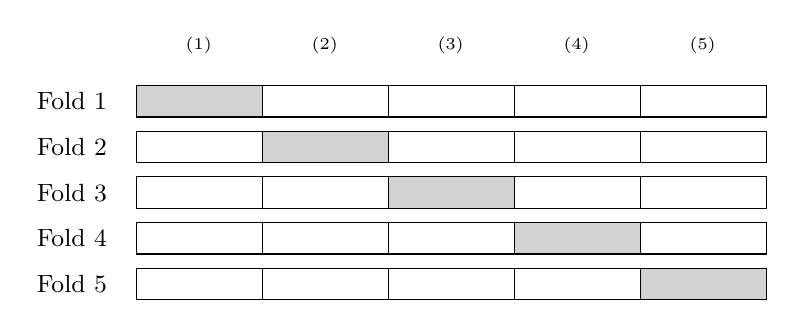
\begin{tikzpicture}[font=\small]
		\def\k{5}          % number of folds
		\def\cellw{1.6}    % width of one segment
		\def\cellh{0.40}   % height of one segment
		\def\gap{0.18}     % vertical gap between rows
		% rows: i = 1..k; columns: j = 1..k
		\foreach \i in {1,...,\k} {
			% row baseline y
			\pgfmathsetmacro{\y}{-(\i-1)*(\cellh+\gap)}
			% row label
			\node[anchor=east] at (-0.25,\y+0.5*\cellh) {Fold \i};
			% draw k equal segments; shade the \i-th as validation
			\foreach \j in {1,...,\k} {
				\pgfmathsetmacro{\x}{(\j-1)*\cellw}
				\ifnum\i=\j
				\fill[gray!35] (\x,\y) rectangle ++(\cellw,\cellh);
				\draw (\x,\y) rectangle ++(\cellw,\cellh);
				\else
				\draw (\x,\y) rectangle ++(\cellw,\cellh);
				\fi
			}
		}
		% add labels D^{(j)} above the columns
		\foreach \j in {1,...,\k} {
			\pgfmathsetmacro{\x}{(\j-1)*\cellw + 0.5*\cellw}
			\node[anchor=south] at (\x,\cellh+0.2) {$\dataset^{(\j)}$};
		}
	\end{tikzpicture}
	\caption{Bei der $k$-fach Kreuzvalidierung wird das verfügbare \gls{dataset} $\dataset$ 
	gleichmäßig in $k$ Folds $\dataset^{(1)},\ldots,\dataset^{(k)}$ unterteilt. 
	Jeder Fold wird einmal als \gls{valset} verwendet, während die verbleibenden $k-1$ Folds 
	das \gls{trainset} bilden.		
	\label{fig_kfoldcv_dict}}
	\end{figure} 
	Für jeden Fold $\foldidx = 1, \,\ldots, \,k$ wird das \gls{model} auf der Vereinigung 
	aller Folds außer $\dataset^{(\foldidx)}$ trainiert und auf 
	$\dataset^{(\foldidx)}$ validiert. Die Gesamtleistung ergibt sich durch Mittelung 
	der \gls{validation}-Ergebnisse über alle $k$ Folds.
	\\ 
	Siehe auch: \gls{validation}, \gls{valerr}.},
	first={$k$-fach Kreuzvalidierung ($k$-fold CV)},
	text={$k$-fold CV} 
}


\newglossaryentry{spectrogram}
{
	name={Spektrogramm},
	description={
		Ein\index{Spektrogramm} Spektrogramm beschreibt die Zeit-Frequenz-Verteilung der Energie eines Zeitsignals $x(t)$. Anschaulich quantifiziert es, wie viel Signalenergie in einem bestimmten Zeitintervall 
		$[t_{1}, t_{2}] \subseteq \mathbb{R}$ und Frequenzbereich $[f_{1}, f_{2}] \subseteq \mathbb{R}$ enthalten ist. 
		
		Formal ist das Spektrogramm eines Signals definiert als das Quadrat des Betrags seiner Kurzzeit-Fourier-Transformation (STFT, short-time Fourier transform) \cite{cohen1995time}.
		
		Abbildung \ref{fig:spectrogram_dict} zeigt ein Zeitsignal zusammen mit seinem Spektrogramm.
		
		\begin{figure}[H]
			\centering
			\includegraphics[width=0.8\textwidth]{assets/spectrogram.png}
			\caption{Links: Ein Zeitsignal bestehend aus zwei modulierten Gauß-Pulsen. Rechts: Ein Intensitätsdiagramm des zugehörigen Spektrogramms.
				\label{fig:spectrogram_dict}}
		\end{figure}
		
		Das Intensitätsbild eines Spektrogramms kann als Bildrepräsentation eines Signals dienen. Ein einfaches Verfahren zur \gls{Klassifikation} von Audiosignalen besteht darin, dieses Signalbild in \gls{DeepNet}s einzuspeisen, die ursprünglich für die Bild-\gls{Klassifikation} und Objekterkennung entwickelt wurden \cite{Li:2022aa}.
		
		Es sei angemerkt, dass es neben dem Spektrogramm noch zahlreiche alternative Darstellungen zur Beschreibung der Zeit-Frequenz-Verteilung der Signalenergie gibt \cite{TimeFrequencyAnalysisBoashash}, \cite{MallatBook}.
	},
	first={Spektrogramm},
	text={Spektrogramm}, plural={Spektogramme}
}

\newglossaryentry{graphclustering}
{
	name={Graph-Clustering},
	description={
		\Gls{Graph}-\gls{Clustering}\index{Graph-Clustering} bezeichnet das \gls{Clustering} von \gls{Datenpunkten}, 
		die als Knoten eines \gls{Graphen} $\graph$ repräsentiert werden. Die Kanten von $\graph$ 
		spiegeln paarweise Ähnlichkeiten zwischen den \gls{Datenpunkten} wider. In manchen Fällen 
		lassen sich diese Ähnlichkeiten durch ein \gls{Kantengewicht} quantitativ beschreiben \cite{FlowSpecClustering2021}, \cite{Luxburg2007}.
	},
	first={Graph-Clustering},
	text={Graph-Clustering}
}


\newglossaryentry{specclustering}
{
	name={Spektrales Clustering},
	description={
		Das spektrale \gls{Clustering}\index{Spektrales Clustering} ist eine spezielle Methode des \gls{GraphClustering}, 
		bei der \gls{Datenpunkte} geclustert werden, die durch die Knoten $\nodeidx = 1, \ldots, \nrnodes$ eines 
		\gls{Graphen} $\graph$ dargestellt werden. 
		
		Beim spektralen \gls{Clustering} werden die \gls{Eigenvektoren} der \gls{LapMat} $\LapMat{\graph}$ verwendet, 
		um \gls{Featurevektoren} $\featurevec^{(\nodeidx)} \in \mathbb{R}^{\nrfeatures}$ für jeden Knoten (also jeden \gls{Datenpunkt}) 
		$\nodeidx=1,\ldots,\nrnodes$ zu konstruieren. Diese \gls{Featurevektoren} können anschließend als Eingabe für 
		\gls{Clustering}-Methoden im \gls{Euklidischen Raum} verwendet werden, z.\,B. \gls{KMeans} oder \gls{SoftClustering} mittels \gls{GMM}. 
		
		Grob gesagt liegen die \gls{Featurevektoren} der Knoten, die zu einer gut verbundenen Teilmenge 
		(also einem \gls{Cluster}) in $\graph$ gehören, im \gls{Euklidischen Raum} $\mathbb{R}^{\nrfeatures}$ nahe beieinander 
		(siehe Abb.~\ref{fig_lap_mtx_specclustering_dict}).
		
		\begin{figure}[H]
			\begin{center}
				\begin{minipage}{0.4\textwidth}
					\begin{tikzpicture}
						\begin{scope}[every node/.style={circle, fill=black, inner sep=0pt, minimum size=0.3cm}]
							\node (1) at (0,0) {};
							\node (2) [below left=of 1, xshift=-0.2cm, yshift=-1cm] {};
							\node (3) [below right=of 1, xshift=0.2cm, yshift=-1cm] {};
							\node (4) [below=of 1, yshift=0.5cm] {};
						\end{scope}
						\draw (1) -- (2);
						\draw (1) -- (3);
						\node[above=0.2cm] at (1) {$\nodeidx=1$};
						\node[left=0.3cm] at (2) {$2$};
						\node[right=0.3cm] at (3) {$3$};
						\node[below=0.2cm] at (4) {$4$};
					\end{tikzpicture}
				\end{minipage}
				\hspace*{5mm}
				\begin{minipage}{0.4\textwidth}
					\begin{equation} 
						\LapMat{\graph} =
						\begin{pmatrix} 
							2 & -1 & -1 & 0 \\ 
							-1 & 1 & 0 & 0 \\  
							-1 & 0 & 1 & 0 \\ 
							0 & 0 & 0 & 0 
						\end{pmatrix}
						= \mathbf{V} {\bm \Lambda} \mathbf{V}^{T}
						\nonumber
					\end{equation}
				\end{minipage}
				\vspace*{20mm}\\
				\begin{minipage}{0.4\textwidth}
					\begin{tikzpicture}[scale=3]
						\draw[->] (-0.2, 0) -- (1.2, 0) node[right] {$v^{(1)}_{\nodeidx}$};
						\draw[->] (0, -0.2) -- (0, 1.2) node[above] {$v^{(2)}_{\nodeidx}$};
						\filldraw[blue] (0.577, 0) circle (0.03cm) node[above right] {$\nodeidx=1,2,3$};
						\filldraw[blue] (0.577, 0) circle (0.03cm);
						\filldraw[blue] (0.577, 0) circle (0.03cm);
						\filldraw[red] (0, 1) circle (0.03cm) node[above right] {$4$};
					\end{tikzpicture}
				\end{minipage}
				\begin{minipage}{0.4\textwidth}
					\begin{align}
						& \mathbf{V} = \big( \vv^{(1)},\vv^{(2)},\vv^{(3)},\vv^{(4)} \big) \nonumber \\
						& \mathbf{v}^{(1)} = \frac{1}{\sqrt{3}} \begin{pmatrix} 1 \\ 1 \\ 1 \\ 0 \end{pmatrix}, \quad
						\mathbf{v}^{(2)} = \begin{pmatrix} 0 \\ 0 \\ 0 \\ 1 \end{pmatrix} \nonumber
					\end{align}
				\end{minipage}
				\caption{\label{fig_lap_mtx_specclustering_dict} 
					{\bf Oben.} Links: Ein ungerichteter \gls{Graph} $\graph$ mit vier Knoten $\nodeidx=1,2,3,4$, 
					die jeweils einen \gls{Datenpunkt} repräsentieren. Rechts: Die \gls{LapMat} 
					$\LapMat{\graph} \in \mathbb{R}^{4 \times 4}$ und ihre \gls{EVD}. 
					{\bf Unten.} Links: Ein \gls{Streudiagramm} der \gls{Datenpunkte} mithilfe der 
					\gls{Featurevektoren} $\featurevec^{(\nodeidx)} = \big( v^{(1)}_{\nodeidx}, v^{(2)}_{\nodeidx} \big)^T$. 
					Rechts: Zwei \gls{Eigenvektoren} $\vv^{(1)}, \vv^{(2)} \in \mathbb{R}^{\nrfeatures}$, 
					die zum \gls{Eigenwert} $\lambda = 0$ der \gls{LapMat} $\LapMat{\graph}$ gehören.
				}
			\end{center}
		\end{figure}
		\newpage
	},
	first={Spektrales Clustering},
	text={Spektrales Clustering}
}


\newglossaryentry{flowbasedclustering}
{
	name={flussbasiertes Clustering},
	description={
		Flussbasiertes \gls{Clustering}\index{flussbasiertes Clustering} gruppiert die Knoten eines 
		ungerichteten \gls{Graphen}, indem \gls{KMeans}-\gls{Clustering} auf knotenspezifische 
		\gls{Featurevektoren} angewendet wird. 
		
		Diese \gls{Featurevektoren} werden aus Netzwerkflüssen konstruiert, die zwischen sorgfältig 
		ausgewählten Quell- und Zielknoten verlaufen \cite{FlowSpecClustering2021}.
	},
	first={flussbasiertes Clustering},
	text={flussbasiertes Clustering}
}

\newglossaryentry{esterr}
{
	name={Schätzfehler},
	description={
		Betrachten wir \gls{Datenpunkte}, jeweils bestehend aus einem \gls{Featurevektor} $\featurevec$ und einem \gls{Label} $\truelabel$. 
		In bestimmten Anwendungen lässt sich die Beziehung zwischen dem \gls{Featurevektor} und dem \gls{Label} 
		eines \gls{Datenpunkts} durch das Modell $\truelabel = \bar{\hypothesis}(\featurevec) + \varepsilon$ beschreiben. 
		Dabei bezeichnet $\bar{\hypothesis}$ eine zugrunde liegende wahre \gls{Hypothese} und $\varepsilon$ 
		einen Rauschterm, der Modellierungs- oder Beschriftungsfehler zusammenfasst. 
		
		Der durch eine \gls{ML}-Methode verursachte **Schätzfehler** ergibt sich bei einer gelernten \gls{Hypothese} 
		$\widehat{\hypothesis}$, z.\,B. mittels \gls{ERM}, als 
		$\widehat{\hypothesis}(\featurevec) - \bar{\hypothesis}(\featurevec)$ für einen gegebenen \gls{Featurevektor}. 
		
		Bei einem parametrischen \gls{Hypothesenraum}, in dem die \gls{Hypothese} durch \gls{Modellparameter} $\weights$ 
		bestimmt ist, lässt sich der Schätzfehler auch durch die Differenz $\Delta \weights = \widehat{\weights} - \overline{\weights}$ 
		ausdrücken \cite{kay}, \cite{hastie01statisticallearning}.
	},
	first={Schätzfehler},
	text={Schätzfehler}
}

\newglossaryentry{dob}
{
	name={Zugehörigkeitsgrad},
	description={
		Der Zugehörigkeitsgrad\index{Zugehörigkeitsgrad} ist eine Kennzahl, die angibt, in welchem Ausmaß ein \gls{Datenpunkt} 
		zu einem bestimmten \gls{Cluster} gehört \cite[Kap.~8]{MLBasics}. Er lässt sich als weiche \gls{Cluster}-Zuordnung interpretieren. 
		
		\Gls{SoftClustering}-Verfahren codieren den Zugehörigkeitsgrad durch eine reelle Zahl im Intervall $[0,1]$. 
		\Gls{HardClustering} stellt den Extremfall dar, bei dem der Zugehörigkeitsgrad nur die Werte $0$ oder $1$ annehmen kann.
	},
	first={Zugehörigkeitsgrad},
	text={Zugehörigkeitsgrad}
}

\newglossaryentry{msee}
{
	name={mittlerer quadratischer Schätzfehler (MSEE)},
	description={
		Der mittlere quadratische Schätzfehler\index{mittlerer quadratischer Schätzfehler (MSEE)} ergibt sich im Kontext einer \gls{ML}-Methode, 
		die \gls{Modellparameter} $\widehat{\weights}$ auf Basis eines \gls{Datensatzes} $\dataset$ erlernt. 
		
		Werden die \gls{Datenpunkte} in $\dataset$ als \gls{iid}-\gls{Realisierungen} einer \gls{Zufallsvariablen} $\datapoint$ interpretiert, 
		so ergibt sich der \gls{Schätzfehler} als $\Delta \weights \defeq \widehat{\weights} - \overline{\weights}$. 
		Dabei bezeichnen $\overline{\weights}$ die wahren \gls{Modellparameter} der \gls{Wahrscheinlichkeitsverteilung} von $\datapoint$. 
		
		Der mittlere quadratische \gls{Schätzfehler} ist definiert als der Erwartungswert $\expect \big\{ \| \Delta \weights \|^{2} \big\}$ 
		der quadrierten euklidischen \gls{Norm} des Schätzfehlers \cite{LC}, \cite{kay}.
	},
	first={mittlerer quadratischer Schätzfehler (MSEE)},
	text={MSEE}
}

\newglossaryentry{gtvmin}
{
	name={Verallgemeinerte Total-Variation-Minimierung (GTVMin)},
	description={
		Die \gls{GTV}-Minimierung\index{Verallgemeinerte Total-Variation-Minimierung (GTVMin)} ist ein Spezialfall der \gls{RERM}, 
		bei dem die \gls{GTV} lokaler \gls{Modellparameter} als \gls{Regularisierer} verwendet wird \cite{ClusteredFLTVMinTSP}.
	},
	first={Verallgemeinerte Total-Variation-Minimierung (GTVMin)},
	text={GTVMin}
}

\newglossaryentry{regression}
{
	name={Regression},
	description={
		Regressionsprobleme\index{Regression} beschäftigen sich mit der Vorhersage eines numerischen \gls{Labels} 
		ausschließlich auf Basis der \gls{Features} eines \gls{Datenpunkts} \cite[Kap.~2]{MLBasics}.
	},
	first={Regression},
	text={Regression}
}
\newglossaryentry{acc}
{
	name={Genauigkeit},
	description={
		Betrachte\index{Genauigkeit} \gls{Datenpunkte}, die durch \gls{Features} $\featurevec \in \featurespace$ 
		und ein kategoriales \gls{Label} $\truelabel$ beschrieben werden, das Werte aus einer endlichen 
		\gls{Labelmenge} $\labelspace$ annimmt. 
		
		Die Genauigkeit einer \gls{Hypothese} $\hypothesis: \featurespace \rightarrow \labelspace$, 
		angewendet auf die \gls{Datenpunkte} eines \gls{Datensatzes} 
		$\dataset = \big\{ \big(\featurevec^{(1)}, \truelabel^{(1)} \big), \ldots, \big(\featurevec^{(\samplesize)},\truelabel^{(\samplesize)}\big) \big\}$, 
		ist definiert als
		\[
		1 - \frac{1}{\samplesize} \sum_{\sampleidx=1}^{\samplesize} 
		\lossfunczo{\big(\featurevec^{(\sampleidx)},\truelabel^{(\sampleidx)}\big)}{\hypothesis}
		\]
		wobei die \gls{0-1-Verlustfunktion} $\lossfunczo{\cdot}{\cdot}$ verwendet wird.
	},
	first={Genauigkeit},
	text={Genauigkeit}
}

\newglossaryentry{expert}
{name={Experte},
	description={ Ein \gls{ml}\index{Experte} zielt darauf ab, eine \gls{hypothesis} $\hypothesis$ zu 			 lernen, die das \gls{label} eines \gls{datapointes} basierend auf dessen \gls{feature}n präzise vorhersagt. 
		Der \gls{prediction}fehler wird mithilfe einer \gls{lossfunc} gemessen. 
		Im Idealfall möchten wir eine \gls{hypothesis} finden, die einen minimalen \gls{loss} 
		für jeden \gls{datapoint} verursacht. Dieses informelle Ziel lässt sich durch die Annahme 
		von \gls{iidasspt} sowie durch die Verwendung des \gls{bayesrisk} als \gls{baseline} für den (durchschnittlichen) 
		\gls{loss} einer \gls{hypothesis} präzisieren. Ein alternativer Ansatz zur Definition einer \gls{baseline} 
		besteht darin, die durch ein bestehendes \gls{ml}-Verfahren gelernte \gls{hypothesis} $\hypothesis'$ zu verwenden. 
		Diese \gls{hypothesis} $\hypothesis'$ bezeichnen wir als *Experten* \cite{PredictionLearningGames}. 
		Methoden zur \gls{regret}-Minimierung lernen eine \gls{hypothesis}, 
		die einen \gls{loss} verursacht, der mit dem des besten Experten vergleichbar ist 
		\cite{PredictionLearningGames}, \cite{HazanOCO}.},
	first={Experte},text={Experte} 
}

\newglossaryentry{nfl}
{name={vernetztes föderiertes Lernen (NFL)},
	description={Vernetztes \gls{fl}\index{vernetztes föderiertes Lernen (NFL)} bezeichnet Methoden, 
		die personalisierte \gls{model}e auf verteilte Weise lernen. 
		Diese Methoden nutzen \gls{localdataset}s, die durch eine intrinsische Netzwerkstruktur miteinander verbunden sind.},
	first={vernetztes föderiertes Lernen (NFL)},text={NFL}
}
%this one is double 

\newglossaryentry{regret}
{name={Regret},
	description={Der \textit{Regret}\index{Regret} einer \gls{hypothesis} $\hypothesis$ relativ zu 
		einer anderen \gls{hypothesis} $\hypothesis'$, die als \gls{baseline} dient, 
		ist die Differenz zwischen dem von $\hypothesis$ verursachten \gls{loss} 
		und dem von $\hypothesis'$ verursachten \gls{loss} \cite{PredictionLearningGames}. 
		Die \gls{baseline}-\gls{hypothesis} $\hypothesis'$ wird auch als \gls{expert} bezeichnet.},
	first={Regret},text={Regret}
	
	\newglossaryentry{strcvx}
	{name={stark konvex},
		description={Eine\index{stark konvex} stetig \gls{differentiable} reellwertige Funktion $f(\featurevec)$ ist 
			stark \gls{convex} mit Koeffizienten $\sigma$, wenn gilt: 
			$f(\vy) \geq f(\vx) + \nabla f(\vx)^{T} (\vy - \vx) + (\sigma/2) \normgeneric{\vy - \vx}{2}^{2}$ 
			\cite{nesterov04}, \cite[Abschnitt B.1.1]{CvxAlgBertsekas}.},
		first={stark konvex},text={stark konvex} 
	}
	
	\newglossaryentry{differentiable}
	{name={differenzierbar},
		description={Eine\index{differenzierbar} reellwertige Funktion $f: \mathbb{R}^{\featuredim} \rightarrow \mathbb{R}$ 
			ist \textit{differenzierbar}, wenn sie an jeder Stelle lokal durch eine lineare Funktion 
			approximiert werden kann. Die lokale lineare Approximation an der Stelle $\mathbf{x}$ 
			wird durch den \gls{gradient} $\nabla f ( \mathbf{x})$ bestimmt 
			\cite{RudinBookPrinciplesMatheAnalysis}.},
		first={differenzierbar},text={differenzierbar} 
	}
	
	\newglossaryentry{gradient}
	{name={Gradient},
		description={Für\index{Gradient} eine reellwertige Funktion $f: \mathbb{R}^{\featuredim} \rightarrow \mathbb{R}: \weights \mapsto f(\weights)$ 
			bezeichnet man einen Vektor $\vg$ als den \emph{Gradienten} von $f$ an der Stelle $\weights'$, 
			wenn gilt: $\lim_{\weights \rightarrow \weights'} \frac{f(\weights) - \big(f(\weights')+ \vg^{T} (\weights- \weights') \big) }{\| \weights-\weights'\|}=0$. 
			Existiert ein solcher Vektor, so wird er mit $\nabla f(\weights')$ oder $\nabla f(\weights)\big|_{\weights'}$ bezeichnet 
			\cite{RudinBookPrinciplesMatheAnalysis}.},
		first={Gradient},text={Gradient}, plural{Gradienten} 
	}

\newglossaryentry{subgradient}
{name={Subgradient},
	description={Für\index{Subgradient} eine reellwertige Funktion $f: \mathbb{R}^{\featuredim} \rightarrow \mathbb{R}: \weights \mapsto f(\weights)$ 
		wird ein Vektor $\va$ als \emph{Subgradient} von $f$ an der Stelle $\weights'$ bezeichnet, 
		wenn gilt: $f(\weights) \geq f(\weights') + \big(\weights - \weights' \big)^{T} \va$ 
		\cite{BertCvxAnalOpt}, \cite{BertsekasNonLinProgr}.},
	first={Subgradient},text={Subgradient} 
}

\newglossaryentry{fedprox}
{name={FedProx},
	description={\textit{FedProx}\index{FedProx} bezeichnet einen iterativen \gls{fl}-\gls{algorithmus}, 
		der zwischen dem separaten Training von \gls{localmodel}s und dem Zusammenführen der aktualisierten lokalen \glspl{modelparam} wechselt. 
		Im Gegensatz zu \gls{fedavg}, das \gls{stochGD} zum Training der \gls{localmodel}s verwendet, 
		nutzt FedProx eine \gls{proxop} für das Training \cite{FedProx2020}.},
	first = {FedProx}, text={FedProx} 
}

\newglossaryentry{relu}
{name={Rectified Linear Unit (ReLU)},
	description={Die\index{Rectified Linear Unit (ReLU)} \textit{ReLU} ist eine häufig verwendete \gls{actfun} 
		in einem künstlichen \gls{ann}-Neuron. Sie ist definiert als 
		$\actfun(z) = \max\{0,z\}$, wobei $z$ den gewichteten Eingang des künstlichen Neurons bezeichnet.},
	first = {Rectified Linear Unit (ReLU)}, text={ReLU} 
}

\newglossaryentry{hypothesis}
{name={Hypothese},
	description={Eine\index{Hypothese} Hypothese bezeichnet eine \gls{map} (oder \gls{function}) 
		$\hypothesis: \featurespace \rightarrow \labelspace$ von dem \gls{featurespace} 
		$\featurespace$ zum \gls{labelspace} $\labelspace$. 
		Für einen \gls{datapoint} mit \glspl{feature} $\featurevec$ verwenden wir eine 
		Hypothese \gls{map} $\hypothesis$, um das \gls{label} $\truelabel$ zu schätzen 
		(oder zu approximieren) mittels der \gls{prediction} 
		$\hat{\truelabel} = \hypothesis(\featurevec)$. 
		\begin{figure}[htbp]
		\centering
			\begin{tikzpicture}[
 		  	>=Latex, node distance=2.0cm,
 		  	box/.style={draw, rounded corners=2pt, inner sep=6pt},
  		 	label/.style={font=\footnotesize},
  		 	thinline/.style={line width=0.6pt}
		 	]
		 	\node[minimum width=3.8cm, minimum height=1.6cm] (audio) {};
		 	\node[label] at (audio.north) [yshift=0mm] {Audiosamples $\featurevec \in \mathbb{R}^{\nrfeatures}$};
		 	\begin{scope}
		 	\draw[thinline]
		 		($(audio.west)+(0.2,0)$) .. controls +(.3,.35) and +(-.3,.35) .. ++(0.8,0)
		 		.. controls +(.3,-.35) and +(-.3,-.35) .. ++(0.8,0)
		 		.. controls +(.3,.25) and +(-.3,.25) .. ++(0.8,0)
		 		.. controls +(.3,-.25) and +(-.3,-.25) .. ++(0.8,0);
		 	\end{scope}
		 	\node[box,right=1.0cm of audio, minimum width=2.2cm, minimum height=1.6cm] (model)
		 	{$\hypothesis$};
		 	\draw[->,thinline] (audio) -- (model) ;
		 	\node[right=1.0cm of model, minimum width=3.2cm, minimum height=1.6cm] (rating) {};
		 	\coordinate (barL) at ($(rating.west)+(0.4,0)$);
		 	\coordinate (barR) at ($(rating.east)+(-0.4,0)$);
		 	\def\score{0.82}
		 	\coordinate (ptr) at ($(barL)!{\score}!(barR)$);
		 	\node[label, above=0pt of ptr] {$\hypothesis(\featurevec)=0.82 (\approx \mbox{Freddie-Level})$};
		 	\draw[->,thinline] (model) -- (rating);
		 	\end{tikzpicture}
			\caption{\label{fig:hypothesis_dict} Eine Hypothese $\hypothesis: \featurespace \rightarrow \labelspace$ 
				mappt die \glspl{feature} $\featurevec \in \featurespace$ eines \gls{datapoint} 
				auf eine \gls{prediction} $\hypothesis(\featurevec) \in \labelspace$ des \gls{label}. 
				Beispielsweise verwendet die \gls{ml}-Anwendung \url{https://freddiemeter.withyoutube.com/} 
				Audioaufnahmen als \glspl{feature}, um vorherzusagen, wie sehr der Gesang einer Person 
				Freddie Mercury ähnelt.
				}
		\end{figure}
		\gls{ml} beschäftigt sich damit, eine Hypothese \gls{map} $\hypothesis$ zu lernen (oder zu finden), 
		sodass $\truelabel \approx \hypothesis(\featurevec)$ für jeden \gls{datapoint} gilt 
		(mit \glspl{feature} $\featurevec$ und \gls{label} $\truelabel$). Praktische \gls{ml}-Methoden, 
		beschränkt durch endliche Rechenressourcen, müssen das Lernen auf eine Teilmenge aller möglichen 
		Hypothesenabbildungen einschränken. Diese Teilmenge wird \gls{hypospace} oder einfach das 
		\gls{model} der Methode genannt.
					\\ 
		Siehe auch: \gls{map}, \gls{function}, \gls{prediction}, \gls{model}.},
	first={Hypothese},
	firstplural={Hypothesen},
	plural={Hypothesen},
	text={Hypothese}  
}

\newglossaryentry{labelspace}
{name={Labelraum},
	description={
		In einer \gls{ml}-Anwendung\index{Labelraum} wird jeder \gls{datapoint} durch eine 
		Menge von \glspl{feature} zusammen mit einem zugehörigen \gls{label} beschrieben. 
		Die Menge aller zulässigen \gls{label}-Werte wird als \gls{labelspace} bezeichnet 
		und mit $\labelspace$ notiert. Wichtig ist, dass $\labelspace$ auch Werte enthalten kann, 
		die kein beobachteter \gls{datapoint} tatsächlich als \gls{label}-Wert aufweist. 
		In großem Maße liegt die Wahl von $\labelspace$ beim \gls{ml}-Ingenieur und hängt von der 
		Problemstellung ab. Abbildung~\ref{fig_label_spaces_dict} zeigt einige Beispiele für \glspl{labelspace}, 
		die häufig in \gls{ml}-Anwendungen verwendet werden.
		\begin{figure}[H]
		\centering
		\begin{tikzpicture}[>=Stealth, font=\small]
			% (a) Reelle Linie für Regression
			\begin{scope}[shift={(0,0)}]
				\draw[->] (-2,0) -- (2,0);
				\node[below=6pt] at (0,-0.7) {(a) $\labelspace\!=\!\mathbb{R}$ (\gls{regression})};
			\end{scope}
			% (b) Ebene für Multi-Label Regression
			\begin{scope}[shift={(7,0)}]
				\fill[gray!20] (-1,-0.5) rectangle (1,0.5);
				\draw[->] (-2,0) -- (2,0);
				\draw[->] (0,-1) -- (0,1);
				\node[below=6pt] at (0,-0.7) {(b) $\labelspace\!=\!\mathbb{R}^{2}$ (Multi-Label \gls{regression})};
			\end{scope}
			% (c) Binäre Klassifikation
			\begin{scope}[shift={(0,-3)}]
				\fill (-1,0) circle (1.2pt) node[below=2pt] {\text{„heiß“}};
				\fill ( 1,0) circle (1.2pt) node[below=2pt] {\text{„kalt“}};
				\node[below=14pt] at (0,-0.7) {(c) $|\labelspace|=2$ Binäre \gls{classification}};
			\end{scope}
			% (d) Ordinale Regression: gerichtete Kette
			\begin{scope}[shift={(7,-3)}]
				\node[circle, inner sep=1pt, draw] (n1) at (-1.5,0) {};
				\node[circle, inner sep=1pt, draw] (n2) at (-0.5,0) {};
				\node[circle, inner sep=1pt, draw] (n3) at ( 0.5,0) {};
				\node[circle, inner sep=1pt, draw] (n4) at ( 1.5,0) {};
				\draw[->] (n1) -- (n2);
				\draw[->] (n2) -- (n3);
				\draw[->] (n3) -- (n4);
				\node[below=2pt of n1] {1};
				\node[below=2pt of n2] {2};
				\node[below=2pt of n3] {3};
				\node[below=2pt of n4] {4};
				\node[below=14pt] at (0,-0.7) {(d) $\labelspace\!=\!\{1,2,3,4\}$ (Ordinale \gls{regression})};
			\end{scope}
		\end{tikzpicture}
		\caption{\label{fig_label_spaces_dict} Beispiele für \glspl{labelspace} und entsprechende Arten von \gls{ml}.}
		\end{figure}
		Die Wahl des \gls{labelspace} $\labelspace$ bestimmt die Art der \gls{ml}-Methoden, 
		die für die jeweilige Anwendung geeignet sind. \Gls{regression}-Methoden verwenden 
		$\labelspace = \mathbb{R}$, während binäre \gls{classification}-Methoden ein \gls{label}-Raum 
		$\labelspace$ mit zwei Elementen verwenden, d.h. $|\labelspace|=2$. Ordinale \gls{regression}-Methoden 
		verwenden eine endliche, geordnete Menge von \gls{label}-Werten, z.B. 
		$\labelspace = \{1,2,3,4\}$ mit der natürlichen Ordnung $1 < 2 < 3 < 4$.
					\\ 
		Siehe auch:  \gls{datapoint}, \gls{label}, \gls{regression}, \gls{classification}.}, 
	first={Labelraum},
	text={Labelraum}  
}

\newglossaryentry{prediction}
{name={Vorhersage}, plural={Vorhersagen},
	description={Eine\index{Vorhersage} Vorhersage ist eine Schätzung oder Approximation einer interessierenden Größe. 
		Das Gebiet des \gls{ml} befasst sich im Wesentlichen mit dem Lernen bzw. Finden einer \gls{hypothesis}-\gls{map} $\hypothesis$, 
		die die \glspl{feature} $\featurevec$ eines \gls{datapoint} einliest und daraus eine Vorhersage 
		$\widehat{\truelabel} \defeq \hypothesis(\featurevec)$ für dessen \gls{label} $\truelabel$ liefert.
					\\ 
		Siehe auch: \gls{ml}, \gls{hypothesis}, \gls{map}, \gls{feature}, \gls{datapoint}, \gls{label}.},
	first={Vorhersage},
	text={Vorhersage},
	plural={Vorhersagen}  
}

\newglossaryentry{empiricaldistribution}
{name = {empirische Verteilung},
description = {Betrachte ein \gls{dataset} 
	$\dataset = \{ \featurevec^{(1)},\ldots, \featurevec^{(\samplesize)}\}$,
	das aus $\samplesize$ verschiedenen \glspl{datapoint} besteht, wobei jeder \gls{datapoint} 
	durch einen \gls{featurevec} $\featurevec^{(\sampleidx)} \in \featurespace$ für 
	$\sampleidx = 1, \ldots, \samplesize$ beschrieben wird. 
	Für eine gegebene \gls{sigmaalgebra} $\sigmaalgebra$ über dem \gls{featurespace} 
	$\featurespace$ ist die empirische Verteilung\index{empirische Verteilung} \cite{Kabluchko2017}
	von $\dataset$ die \gls{probdist} $\probdist$, die definiert ist durch
	$$\probdist(\mathcal{A}) = (1/\samplesize)\, \big| \big\{ \sampleidx : \featurevec^{(\sampleidx)} \in \mathcal{A} \big\} \big|, 
	\quad \text{für alle } \mathcal{A} \in \sigmaalgebra.$$
	Mit anderen Worten weist die empirische Verteilung jeder \gls{messbare}n Menge 
	$\mathcal{A} \in \sigmaalgebra$ den Anteil der \glspl{datapoint} in $\dataset$ zu, 
	die in $\mathcal{A}$ liegen. 
	Ist der \gls{featurespace} geordnet, so kann die empirische Verteilung auch durch ihre empirische 
	\gls{cdf} charakterisiert werden:
	$$\cdf{\dataset}{\featurevec} = 
	(1/\samplesize)\, \big| \big\{ \sampleidx : \featurevec^{(\sampleidx)} \preceq \featurevec \big\} \big|, 
	\quad \text{für alle } \featurevec \in \featurespace,$$
	wobei $\preceq$ die Ordnungsrelation auf $\featurespace$ bezeichnet.
	\begin{figure}[H]
	\begin{center}
	\begin{tikzpicture}[>=stealth, thick,y=2cm]
		\foreach \x/\p in {1/0.3, 4/0.7}
		{% Stabdiagramm
		\draw[gray] (\x,0) -- (\x,\p);
		\fill[blue] (\x,\p) circle (2pt);
		}
		\node[anchor=south,align=center] at (1,0.3) {\small $\pmf{\dataset}{\star}=3/10$};
		\node[anchor=north] at (1,0) {\small $\star$};
		\node[anchor=north] at (4,0) {\small $\otimes$};
		\node[anchor=west,text width=11cm] at (-1.2,-0.80) {
			$\dataset = (\star,\star,\star,\otimes,\otimes,\otimes,\otimes,\otimes,\otimes,\otimes)$
		};
	\end{tikzpicture}
	\end{center}
	\caption{Ein \gls{dataset} $\dataset$ mit $\samplesize = 10$ \glspl{datapoint}, 
	die jeweils einen Wert aus dem endlichen \gls{featurespace} 
	$\featurespace = \{\star, \otimes\}$ annehmen. 
	Die empirische \gls{pmf} $\pmf{\dataset}{\featurevec}$ ordnet jedem möglichen Wert 
	$\featurevec \in \featurespace$ den Anteil der \glspl{datapoint} in $\dataset$ zu, 
	deren \gls{feature} diesen Wert annimmt. Hier nehmen drei von zehn \glspl{datapoint} 
	den \gls{feature}-Wert $\star$ an, was zu $\pmf{\dataset}{\star} = 3/10$ führt. 
	\label{fig_empirical_pmf_dict}}
	\end{figure}
	Ist der \gls{featurespace} $\featurespace$ endlich, 
	kann die empirische Verteilung von $\dataset$ auch durch die empirische 
	\gls{pmf} charakterisiert werden:
	$$\pmf{\dataset}{\featurevec} = 
	(1/\samplesize)\, \big| \big\{ \sampleidx : \featurevec^{(\sampleidx)} = \featurevec \big\} \big|, 
	\quad \text{für alle } \featurevec \in \featurespace.$$
	\\
	Siehe auch: \gls{probdist}, \gls{sigmaalgebra}.},
	type = {math},
	text = {empirische Verteilung},
 	plural = {empirische Verteilungen},
	 first = {empirische Verteilung},
 	
}

\newglossaryentry{histogram}
{name={Histogramm},
 description={Betrachte\index{Histogramm} ein \gls{dataset} $\dataset$, das aus 
 $\samplesize$ \glspl{datapoint} $\datapoint^{(1)}, \,\ldots, \,\datapoint^{(\samplesize)}$ besteht, 
 wobei jedes dieser Elemente zu einer Zelle $[-U,U] \times \ldots \times [-U,U] \subseteq \mathbb{R}^{\featuredim}$ 
 mit Kantenlänge $U$ gehört. Diese Zelle wird gleichmäßig in kleinere, elementare Zellen mit 
 Kantenlänge $\Delta$ unterteilt. Das Histogramm von $\dataset$ ordnet jeder dieser 
 elementaren Zellen den entsprechenden Anteil der \glspl{datapoint} in $\dataset$ zu, 
 die in diese Zelle fallen. Ein visuelles Beispiel eines solchen Histogramms ist in 
 Abbildung~\ref{fig:histogram_dict} dargestellt.\\
 \begin{figure}[H]
 \centering
 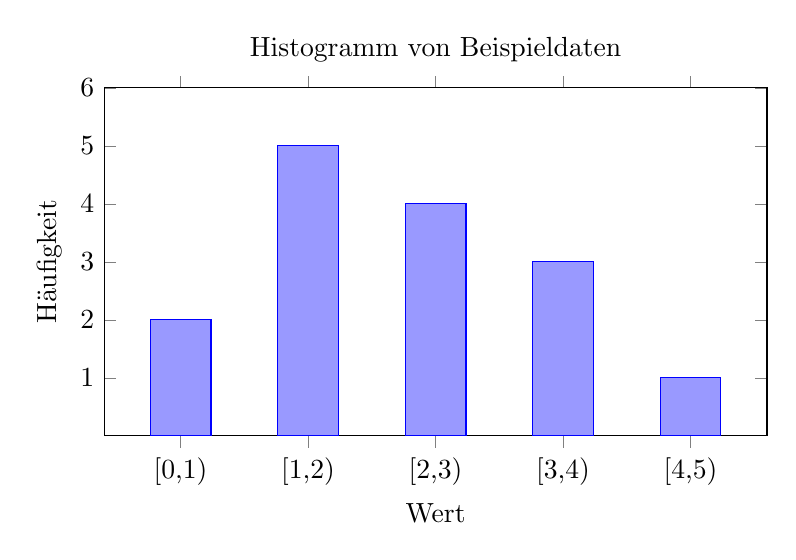
\begin{tikzpicture}
 \pgfplotsset{compat=1.18}
 \begin{axis}[
     ybar,
     ymin=0,
     ymax=6,
     bar width=22pt,
     width=10cm,
     height=6cm,
     xlabel={Wert},
     ylabel={Häufigkeit},
     ytick={1,2,3,4,5,6},
     xtick={1,2,3,4,5},
     xticklabels={{[0,1)}, {[1,2)}, {[2,3)}, {[3,4)}, {[4,5)}},
     enlarge x limits=0.15,
     title={Histogramm von Beispieldaten}
     ]
 \addplot+[fill=blue!40] coordinates {(1,2) (2,5) (3,4) (4,3) (5,1)};
 \end{axis}
 \end{tikzpicture}
 \caption{Ein Histogramm zeigt die Anteile der \glspl{datapoint}, 
 die in verschiedene Wertebereiche (sogenannte Bins) fallen. 
 Die Höhe jedes Balkens gibt die Anzahl der \glspl{sample} im entsprechenden Intervall an.}
 \label{fig:histogram_dict}
 \end{figure}
 Siehe auch: \gls{dataset}, \gls{datapoint}, \gls{sample}.},
 first={Histogramm},
 text={Histogramm},
 plutal={Histogramme}
}

\newglossaryentry{bootstrap}
{name={Bootstrap},
	description={Zur\index{Bootstrap} Analyse von \gls{ml}-Methoden ist es oft hilfreich, 
	ein gegebenes Set von \glspl{datapoint} 
	$\dataset = \big\{ \datapoint^{(1)}, \,\ldots, \,\datapoint^{(\samplesize)}\big\}$ 
	als \glspl{realization} unabhängiger und identisch verteilter (\gls{iid}) \glspl{rv} 
	aufzufassen, die aus einer gemeinsamen \gls{probdist} $\probdist$ gezogen wurden. 
	In der Praxis ist die zugrundeliegende Verteilung $\probdist$ jedoch unbekannt und 
	muss aus den Daten geschätzt werden. Der Bootstrap-Ansatz verwendet das 
	\gls{histogram} von $\dataset$ als Schätzer für $\probdist$ 
	\cite{hastie01statisticallearning}, 
	$$ (1/\samplesize) \big| \{ \sampleidx : \datapoint^{(\sampleidx)} \in \mathcal{A} \} \big| 
	\approx \prob{\mathcal{A}}.$$
	Durch Ziehen mit Zurücklegen aus $\dataset$ entsprechend dieser empirischen Verteilung 
	werden neue \glspl{dataset} 
	$\dataset^{(1)}, \ldots, \dataset^{(\nrbootstraps)}$ erzeugt, 
	von denen jedes $\samplesize$ \glspl{datapoint} enthält. 
	Jedes dieser Datensätze wird anschließend zur \gls{model}-\gls{training} 
	verwendet (z.\,B. mittels \gls{erm}), 
	wodurch die gelernten \glspl{hypothesis} 
	$\widehat{\hypothesis}^{(1)}, \ldots, \widehat{\hypothesis}^{(\nrbootstraps)}$ entstehen. 
	Diese gelernten \glspl{hypothesis} können anschließend genutzt werden, 
	um die \gls{stability} der jeweiligen \gls{ml}-Methode zu bewerten 
	\cite{hastie01statisticallearning}.
	\\
	Siehe auch: \gls{iid}, \gls{rv}, \gls{probdist}, \gls{histogram}.},
	first={Bootstrap},
	text={Bootstrap}  
}

\newglossaryentry{featurespace}
{name={Merkmalsraum},
	description={Der\index{Merkmalsraum} \gls{feature}-Raum
	 (auch feature space)einer gegebenen \gls{ml}-Anwendung 
		oder Methode besteht aus allen möglichen Werten, die der \gls{featurevec} eines \gls{datapoint} 
		annehmen kann. Für \glspl{datapoint}, die durch eine feste Anzahl $\nrfeatures$ numerischer \glspl{feature} beschrieben werden, 
		ist eine gängige Wahl für den \gls{feature}-Raum der \gls{euclidspace} $\mathbb{R}^{\nrfeatures}$. 
		Die bloße Existenz von $\nrfeatures$ numerischen \glspl{feature} bedeutet jedoch nicht, dass $\mathbb{R}^{\nrfeatures}$ 
		die geeignetste Darstellung des \gls{feature}-Raums ist. Tatsächlich könnten die numerischen \glspl{feature} 
		den \glspl{datapoint} in weitgehend willkürlicher oder zufälliger Weise zugeordnet sein, 
		was zu \glspl{datapoint} führt, die zufällig in $\mathbb{R}^{\nrfeatures}$ verteilt sind, 
		ohne eine sinnvolle geometrische Struktur. Methoden des \gls{featlearn} versuchen, 
		eine Transformation der ursprünglichen (potenziell nicht-numerischen) \glspl{feature} zu erlernen, 
		um eine sinnvollere Anordnung der \glspl{datapoint} in $\mathbb{R}^{\nrfeatures}$ zu erreichen. 
		Drei Beispiele für \gls{feature}-Räume sind in Abb. \ref{fig_featurespace_dict} dargestellt.
		\begin{figure}[H]
			\centering
			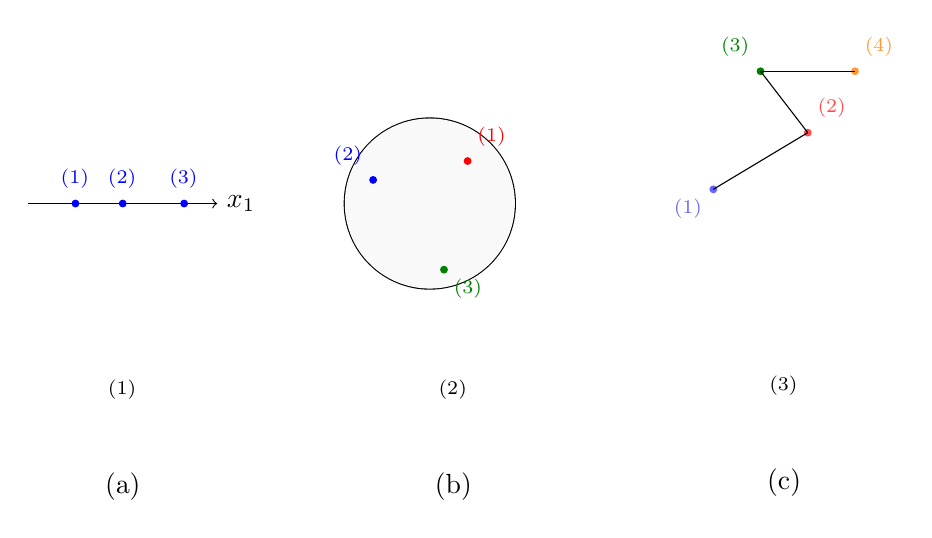
\begin{tikzpicture}[scale=0.6]
			% --------- 1D Line Feature Space (left) ---------
			\begin{scope}[xshift=0cm]
  				% Axis
 	 			\draw[->] (-0.5, 0) -- (3.5, 0) node[right] {$x_1$};
  				% Points
  				\foreach \x/\lbl in {0.5/$\featurevec^{(1)}$, 1.5/$\featurevec^{(2)}$, 2.8/$\featurevec^{(3)}$}
    				\filldraw[blue] (\x,0) circle (2pt) node[above] {\lbl};
  				% Label
  				\node at (1.5, -4.0)  {$\featurespace^{(1)}$};
				\node at (1.5, -6) {(a)};
			\end{scope}
			% --------- 2-D Bounded (Disk) Feature Space (middle) ---------
			\begin{scope}[xshift=8cm]
  				% Circle boundary
  				\draw[thick] (0,0) circle (1.8);
  				\fill[gray!5] (0,0) circle (1.8);
  				% Points inside circle
  				\filldraw[red] (0.8, 0.9) circle (2pt) node[anchor=south west] {$\featurevec^{(1)}$};
  				\filldraw[blue] (-1.2, 0.5) circle (2pt) node[anchor=south east] {$\featurevec^{(2)}$};
  				\filldraw[green!50!black] (0.3, -1.4) circle (2pt) node[anchor=north west] {$\featurevec^{(3)}$};
  				% Label
  				\node at (0.5, -4) {$\featurespace^{(2)}$};
				\node at (0.5, -6) {(b)};
			\end{scope}
			% --------- Graph-Based Feature Space (right) ---------
			\begin{scope}[xshift=14cm, yshift=0.3cm]
  				% Nodes
 	 			\filldraw[blue!60] (0,0) circle (2pt) node[anchor=north east] {$\featurevec^{(1)}$};
 	 			\filldraw[red!70] (2,1.2) circle (2pt) node[anchor=south west] {$\featurevec^{(2)}$};
  				\filldraw[green!50!black] (1,2.5) circle (2pt) node[anchor=south east] {$\featurevec^{(3)}$};
  				\filldraw[orange!80] (3,2.5) circle (2pt) node[anchor=south west] {$\featurevec^{(4)}$};
  				% Edges
  				\draw[-] (0,0) -- (2,1.2);
  				\draw[-] (2,1.2) -- (1,2.5);
  				\draw[-] (1,2.5) -- (3,2.5);
  				% Label
  				\node at (1.5, -4.2) {$\featurespace^{(3)}$};
				\node at (1.5, -6.2) {(c)};
			\end{scope}
			\end{tikzpicture}
		\caption{Drei unterschiedliche \gls{feature}-Räume. (a) Ein linearer Raum $\featurespace^{(1)} = \mathbb{R}$. (b) Eine 
		beschränkte \gls{convex}-Menge $\featurespace^{(2)} \subseteq \mathbb{R}^{2}$. (c) Ein diskreter Raum 
		$\featurespace^{(3)}$, dessen Elemente Knoten eines ungerichteten \gls{graph} sind. \label{fig_featurespace_dict}}
		\end{figure}
		Siehe auch: \gls{featurevec}, \gls{euclidspace}.},
	first={Merkmalsraum},
	text={Merkmalsraum}  
}


\newglossaryentry{missingdata}
{name={fehlende Daten},
	description={Betrachten wir\index{fehlende Daten} ein \gls{dataset}, das aus \glspl{datapoint} besteht, die 
		mittels eines physikalischen \gls{device} erhoben wurden. Aufgrund von Unvollkommenheiten oder Ausfällen 
		könnten einige \gls{feature}- oder \gls{label}-Werte von \glspl{datapoint} beschädigt oder einfach 
		fehlend sein. Die \gls{data}-Imputation zielt darauf ab, diese fehlenden Werte zu schätzen \cite{Abayomi2008DiagnosticsFM}. 
		Man kann \gls{data}-Imputation als ein \gls{ml}-Problem interpretieren, bei dem das \gls{label} eines \gls{datapoint} 
		der Wert des beschädigten \gls{feature} ist.
		\\
		Siehe auch: \gls{feature}, \gls{label}. },
	first={fehlende Daten},
	text={fehlende Daten}  
}


\newglossaryentry{psd}
{name={positiv semidefinit (psd)},
	description={Eine\index{positiv semidefinit (psd)} (reellwertige) symmetrische \gls{matrix} 
	 	$\mQ = \mQ\,^{T} \in \mathbb{R}^{\featuredim \times \featuredim}$ 
	 	ist positiv semidefinit (psd), wenn $\featurevec\,^{T} \mQ \featurevec \geq 0$ 
	 	für jeden \gls{vector} $\featurevec \in \mathbb{R}^{\featuredim}$ gilt. 
	 	Die Eigenschaft der PSD kann von \glspl{matrix} auf (reellwertige) symmetrische 
	 	\gls{kernel}-\glspl{map} $\kernel: \featurespace \times \featurespace \rightarrow \mathbb{R}$ 
	 	(mit $\kernel(\featurevec,\featurevec') = \kernel(\featurevec',\featurevec)$) erweitert werden: 
	 	Für jede endliche Menge von \glspl{featurevec} $\featurevec^{(1)}, \ldots, \featurevec^{(\samplesize)}$ 
	 	ist die resultierende \gls{matrix} $\mQ \in \mathbb{R}^{\samplesize \times \samplesize}$ mit 
		Einträgen $Q_{\sampleidx,\sampleidx'} = \kernelmap{\featurevec^{(\sampleidx)}}{\featurevec^{(\sampleidx')}}$ 
		psd \cite{LearningKernelsBook}.
		\\
		Siehe auch: \gls{matrix}, \gls{vector}, \gls{kernel}, \gls{map}, \gls{featurevec}.},
	first={positiv semidefinit (psd)},
	text={psd}  
}


\newglossaryentry{feature}
{name={Feature}, plural={Features},
description={Ein\index{Feature} Feature eines \gls{datapoint} ist eine seiner Eigenschaften, 
    die leicht messbar oder berechenbar ist, ohne dass menschliche Aufsicht erforderlich ist. 
    Beispielsweise kann, wenn ein \gls{datapoint} ein digitales Bild (z.\,B. gespeichert als \texttt{.jpeg}-Datei) ist, 
    die Rot–Grün–Blau-(RGB-)Intensität seiner Pixel als Features verwendet werden. 
    \begin{figure}
    \centering
    \begin{tikzpicture}[scale=1]
    % Glatte Wellenform zeichnen (Sinuskurve als Beispiel für ein Audiosignal)
    \draw[thick, blue, domain=0:6.28, smooth, variable=\x] 
        plot ({\x}, {sin(\x r)});
    % Probenpunkte in regelmäßigen Abständen markieren
    \foreach \x [count=\i] in {0,0.5,...,6.28} {
        \fill[red] (\x, {sin(\x r)}) circle (2pt);
        % Nur die ersten beiden Proben beschriften
        \ifnum\i=1
            \node[above left] at (\x, {sin(\x r)}) {$x_1$};
        \fi
        \ifnum\i=2
            \node[above left] at (\x, {sin(\x r)}) {$x_2$};
        \fi
    }
    \end{tikzpicture}
    \caption{Ein Audiosignal (blaue Wellenform) und seine diskretisierten Signalproben (rote Punkte), 
    die als Features $x_{1},\ldots,x_{\nrfeatures}$ verwendet werden können. \label{fig:audio_features_dict}}
    \end{figure}
    Ein weiteres Beispiel zeigt Abb.\ \ref{fig:audio_features_dict}, in der die Signalproben eines Audiosignals endlicher Dauer als Features genutzt werden.
    Fachspezifische Synonyme für den Begriff Feature sind „Kovariate“, „erklärende Variable“, 
    „unabhängige Variable“, „Input-Variable“, „Prädiktor“ oder „Regressor“ \cite{Gujarati2021}, \cite{Dodge2003}, \cite{Everitt2010}. 
        \\
    Siehe auch: \gls{datapoint}.},
first={Feature},
text={Feature}  
}

\newglossaryentry{featurevec}
{name={Featurevektor}, plural={Featurevektoren},
description={Ein \Gls{feature} \gls{vector} bezeichnet einen\index{Featurevektor} \gls{Vektor} 
    $\vx = \big(x_{1}, \,\ldots, \,x_{\nrfeatures}\big)\,^{T}$, dessen Einträge die einzelnen \glspl{feature} 
    $x_{1}, \,\ldots, \,x_{\nrfeatures}$ darstellen. Viele \gls{ml}-Methoden verwenden \gls{feature} \glspl{vector}, 
    die in einem endlichdimensionalen \gls{euclidspace} $\mathbb{R}^{\nrfeatures}$ liegen. 
    Für bestimmte \gls{ml}-Methoden kann es jedoch zweckmäßiger sein, mit \gls{feature} \glspl{vector} zu arbeiten, 
    die einem unendlichdimensionalen \gls{vectorspace} angehören (z.\,B. siehe \gls{kernelmethod}). 
        \\
    Siehe auch: \gls{feature}, \gls{vector}, \gls{ml}, \gls{euclidspace}, \gls{vectorspace}.}, 
first={Featurevektor},
text={Featurevektor}  
}

\newglossaryentry{label}
{name={Label}, plural={Labels},
description={Ein\index{Label} Label ist eine höherwertige Information oder eine Zielgröße, die einem \gls{datapoint} zugeordnet ist. 
    Beispielsweise könnte bei einem Bild als \gls{datapoint} das Label angeben, ob das Bild eine Katze enthält oder nicht. 
    Synonyme für Label, die in spezifischen Fachgebieten gebräuchlich sind, sind „Antwortvariable“, „Ausgabevariable“ oder „Target“ \cite{Gujarati2021}, \cite{Dodge2003}, \cite{Everitt2010}. 
        \\
    Siehe auch: \gls{datapoint}, \gls{labelspace}.},
first={Label},
text={Label}  
}

\newglossaryentry{data}
{name={Daten},
description={Im Kontext von \gls{ml} wird der Begriff 
Daten\index{Daten} häufig synonym mit \gls{dataset} verwendet
\cite{Everitt2010,OxfordStatisticsDictionary}. 
Der ISO/IEC 2382:2015 Standard definiert Daten als eine \emph{neu interpretierbare Darstellung von 
Informationen in formalisierter Weise, geeignet für Kommunikation, Interpretation 
oder Verarbeitung} \cite{ISO2382}. 
  \\
  Siehe auch: \gls{dataset}, \gls{datapoint}, \gls{sample}.}, 
text={Daten}
}



\newglossaryentry{dataset}
{name={Datensatz}, plural={Datensätze},
description={Ein\index{Datensatz} Datensatz ist eine Menge von unterschiedlichen \glspl{datapoint}. 
Streng genommen ist ein Datensatz eine ungeordnete Sammlung von \glspl{datapoint}, 
die keine Wiederholungen enthält. In der Praxis wird der Begriff Datensatz jedoch oft 
als Synonym für eine \gls{sample} verwendet, d.h. eine Sequenz (oder endliche Liste) 
von \glspl{datapoint}, die Wiederholungen enthalten kann. 
\gls{ml}-Methoden verwenden Datensätze, um \glspl{model} zu trainieren und zu validieren. 
Der Begriff Datensatz ist weit gefasst: \glspl{datapoint} können konkrete physische 
Entitäten (z. B. Menschen oder Tiere) oder abstrakte Objekte (z. B. Zahlen) darstellen. 
Zur Illustration zeigt Abbildung~\ref{fig_cows_dataset_dict} einen Datensatz, dessen 
\glspl{datapoint} Kühe sind.
	\begin{figure}[H]
		\begin{center}
		\label{fig:cowsintheswissalps_dict}
		\includegraphics[width=0.5\textwidth]{assets/CowsAustria.jpg}
	  	\end{center}
		\caption{\label{fig_cows_dataset_dict}Eine Kuhherde irgendwo in den Alpen.}
 	\end{figure}
Oft hat ein \gls{ml}-Ingenieur keinen direkten Zugriff auf den zugrunde liegenden Datensatz. 
Zum Beispiel würde der Zugriff auf den Datensatz in Abbildung~\ref{fig_cows_dataset_dict} 
einen Besuch der Kuhherde erfordern. In der Praxis arbeitet man mit einer praktischeren 
Darstellung (oder Approximation) des Datensatzes. Hierfür wurden verschiedene 
mathematische \glspl{model} entwickelt \cite{silberschatz2019database}, \cite{abiteboul1995foundations}, 
\cite{hoberman2009data}, \cite{ramakrishnan2002database}. Eines der am weitesten verbreiteten 
Modelle ist das relationale \gls{model}, das \gls{data} in Tabellenform (Relationen) organisiert 
\cite{codd1970relational}, \cite{silberschatz2019database}. Eine Tabelle besteht aus 
Zeilen und Spalten: Jede Zeile entspricht einem einzelnen \gls{datapoint}, jede 
Spalte stellt ein bestimmtes Attribut eines \gls{datapoint} dar. 
\gls{ml}-Methoden interpretieren diese Attribute typischerweise als \glspl{feature} 
oder als \gls{label} eines \gls{datapoint}. Zur Illustration zeigt Tabelle~\ref{tab:cowdata_dict} 
eine relationale Darstellung des Datensatzes aus Abbildung~\ref{fig_cows_dataset_dict}. 
Im relationalen \gls{model} ist die Reihenfolge der Zeilen unerheblich, und jedes Attribut 
(Spalte) ist mit einer Domäne verknüpft, die die Menge der zulässigen Werte spezifiziert. 
In \gls{ml}-Anwendungen entsprechen diese Attribut-Domänen dem \gls{featurespace} und dem 
\gls{labelspace}.
\begin{table}[H]
	\refstepcounter{table}
	\caption*{
		\centering 
		\scshape TABELLE \thetable \\[0.5ex]
		\scshape Eine Relation (Tabelle), die den Datensatz in Abbildung \ref{fig_cows_dataset_dict} darstellt 
	}
	\label{tab:cowdata_dict} 
	\centering
	\begin{tabular}{lcccc}
		\hline
		\textbf{Name} & \textbf{Gewicht} & \textbf{Alter} & \textbf{Größe} & \textbf{Magentemperatur} \\
		\hline
		Zenzi & 100 & 4 & 100 & 25 \\
		Berta & 140 & 3 & 130 & 23 \\
		Resi  & 120 & 4 & 120 & 31 \\
		\hline
	\end{tabular}
\end{table}
Während das relationale \gls{model} für viele \gls{ml}-Anwendungen nützlich ist, 
kann es für Anforderungen im Bereich \gls{trustAI} unzureichend sein. Moderne Ansätze, 
wie „Datasheets for Datasets“, bieten eine umfassendere Dokumentation, 
einschließlich Details zum \gls{data}-Erhebungsprozess, dem vorgesehenen Verwendungszweck 
und weiteren Kontextinformationen \cite{DatasheetData2021}.
\\
Siehe auch: \gls{datapoint}, \gls{data}, \gls{feature}, \gls{sample}, \gls{featurespace}, \gls{labelspace}.},
text={Datensatz}
}



\newglossaryentry{predictor}
{name={Vorhersagefunktion},
description={Eine\index{Vorhersagefunktion} Vorhersagefunktion ist eine reellwertige Abbildung (\gls{hypothesis}-\gls{map}),
 die aus den \glspl{feature} eines \gls{datapoint} eine Vorhersage für dessen numerisches \gls{label} $\truelabel \in \mathbb{R}$ erzeugt. 
Formal gilt: Für ein \gls{datapoint} mit \glspl{feature} $\featurevec$ liefert die Vorhersagefunktion $\hypothesis(\featurevec) \in \mathbb{R}$ 
eine Schätzung des wahren Labels.
\\
Siehe auch: \gls{hypothesis}, \gls{map}, \gls{datapoint}, \gls{feature}, \gls{prediction}, \gls{label}.},
text={Vorhersagefunktion}
}



\newglossaryentry{labeled datapoint}
{name={gelabelter Datenpunkt}, plural={gelabelte Datenpunkte},
description={Ein\index{gelabelter Datenpunkt} \gls{datapoint}, dessen \gls{label} bekannt ist oder 
durch ein Verfahren bestimmt wurde, das menschliche Arbeit erfordern kann.
\\
Siehe auch: \gls{datapoint}, \gls{label}.},
text={gelabelter Datenpunkt}
}

\newglossaryentry{discreteRV}
{name={diskrete Zufallsvariable}, plural={diskrete Zufallsvariablen},
description={Eine\index{diskrete Zufallsvariable} \gls{rv}, d.h. eine \gls{function}, die die 
Ausgänge eines \gls{randomexperiment} auf Elemente eines \gls{measurable} Raums 
$\featurespace$ abbildet, wird als diskret bezeichnet, wenn ihr Wertebereich $\featurespace$ 
abzählbar ist \cite{BillingsleyProbMeasure}.
\\
Siehe auch: \gls{probability}, \gls{rv}, \gls{probdist}.},
text={diskrete Zufallsvariable}
}

\newglossaryentry{rv}
{name={zufällige Variable (RV)}, plural={RVs},
description={Eine RV\index{zufällige Variable (RV)} ist eine \gls{function}, die die 
Ausgänge eines \gls{randomexperiment} auf Elemente eines \gls{measurable} Raums abbildet 
\cite{BillingsleyProbMeasure,GrayProbBook}. 
Mathematisch ist eine RV eine Abbildung $x: \samplespace \rightarrow \featurespace$, 
wobei die Definitionsmenge der \gls{samplespace} $\samplespace$ eines \gls{probspace} 
und die Zielmenge ein \gls{measurable} Raum $\featurespace$ ist. 
Es gibt verschiedene Typen von RVs:
\begin{itemize}
    \item {binäre RVs}, die jedes Ergebnis auf ein Element einer binären Menge abbilden (z.\,B. $\{-1,1\}$ oder $\{\text{Katze}, \text{keine Katze}\}$);
    \item {diskrete RVs}, die Werte in einer abzählbaren Menge annehmen (endlich oder abzählbar unendlich);
    \item {reellwertige RVs}, die Werte in den reellen Zahlen $\mathbb{R}$ annehmen;
    \item {\gls{vector}-wertige RVs}, die Ergebnisse in den \gls{euclidspace} $\mathbb{R}^{\featuredim}$ abbilden.
\end{itemize}
Die \gls{probability}-Theorie verwendet das Konzept der \gls{measurable} Räume, um Eigenschaften von Mengen von RVs rigoros zu definieren und zu untersuchen \cite{BillingsleyProbMeasure}.
\\
Siehe auch: \gls{function}, \gls{randomexperiment}, \gls{samplespace}, \gls{probspace}, \gls{vector}, \gls{euclidspace}, \gls{probability}, \gls{measurable}.},
first={zufällige Variable (RV)},
firstplural={zufällige Variablen (RVs)},
plural={RVs},
text={RV}
}

\newglossaryentry{probspace}
{name={Wahrscheinlichkeitsraum}, 
description={Ein\index{Wahrscheinlichkeitsraum} Wahrscheinlichkeitsraum ist eine mathematische Struktur, die es erlaubt, über ein \gls{randomexperiment} nachzudenken, z.\,B. die Beobachtung eines physikalischen Phänomens. 
Formal ist ein \gls{probability} Raum $\mathcal{P}$ ein Tripel $(\samplespace, \eventspace, \prob{\cdot})$, wobei
\begin{itemize}
    \item $\samplespace$ die \gls{samplespace} ist, die alle möglichen Ausgänge des \gls{randomexperiment} enthält;
    \item $\eventspace$ eine \gls{sigmaalgebra} ist, d.\,h. eine Menge von Teilmengen von $\samplespace$ (genannt \glspl{event}), die bestimmte Abschluss-Eigenschaften unter Mengenoperationen erfüllt;
    \item $\prob{\cdot}$ eine \gls{probdist} ist, d.\,h. eine \gls{function}, die jedem \gls{event} $\mathcal{A} \in \eventspace$ eine Wahrscheinlichkeit $P(\mathcal{A}) \in [0,1]$ zuordnet. Diese \gls{function} muss $\prob{\samplespace} = 1$ und $\prob{\bigcup_{i=1}^{\infty} \mathcal{A}_i} = \sum_{i=1}^{\infty} \prob{\mathcal{A}_i}$ für jede abzählbare Folge paarweise disjunkter \glspl{event} $\mathcal{A}_1, \mathcal{A}_2, \ldots \in \mathcal{F}$ erfüllen.
\end{itemize}
\glspl{probability} Räume bilden die Grundlage für \glspl{probmodel}, mit denen das Verhalten von \gls{ml}-Methoden untersucht werden kann \cite{BillingsleyProbMeasure, GrayProbBook, ross2013first}.
\\
Siehe auch: \gls{probability}, \gls{randomexperiment}, \gls{samplespace}, \gls{event}, \gls{probdist}, \gls{function}, \gls{probmodel}, \gls{ml}.},
first={Wahrscheinlichkeitsraum}, 
text={Wahrscheinlichkeitsraum}
}

\newglossaryentry{samplespace}
{name={Ergebnismenge}, 
description={Eine\index{Ergebnismenge} Ergebnismenge ist die Menge aller möglichen Ausgänge eines \gls{randomexperiment} \cite{BillingsleyProbMeasure, BertsekasProb, papoulis, AshProbMeasure}.
\\
Siehe auch: \gls{probspace}.},
first={Ergebnismenge}, 
firstplural={Ergebnismengen},
plural={Ergebnismengen},
text={Ergebnismenge}
}

\newglossaryentry{samplespace}
{name={Ergebnismenge}, 
description={Eine\index{Ergebnismenge} Ergebnismenge ist die Menge aller möglichen Ausgänge eines \gls{randomexperiment} \cite{BillingsleyProbMeasure, BertsekasProb, papoulis, AshProbMeasure}.
\\
Siehe auch: \gls{probspace}.},  
first={Ergebnismenge}, 
firstplural={Ergebnismengen},
plural={Ergebnismengen},
text={Ergebnismenge}
}

\newglossaryentry{realization}
{name={Realisierung}, plural={Realisierungen},
description={Betrachten wir\index{Realisierung} eine \gls{rv} $\featurevec$, die jeden Ausgang 
$\outcome \in \samplespace$ eines \gls{probspace} auf ein Element $a$ eines \gls{measurable} Raums $\mathcal{N}$ abbildet \cite{RudinBookPrinciplesMatheAnalysis, BillingsleyProbMeasure, HalmosMeasure}. 
Eine Realisierung von $\featurevec$ ist jedes Element $\va \in \mathcal{N}$, für das ein Ausgang $\outcome' \in \samplespace$ existiert, sodass $\featurevec(\outcome') = \va$ gilt.
\\
Siehe auch: \gls{rv}, \gls{probspace}, \gls{measurable}.}, 
first={Realisierung},
text={Realisierung}  
}

\newglossaryentry{trainset}
{name={Trainingsmenge}, plural={Trainingsmengen},
description={Eine\index{Trainingsmenge} Trainingsmenge ist ein \gls{dataset} $\dataset$, das aus einigen \glspl{datapoint} besteht und 
im Rahmen von \gls{erm} verwendet wird, um eine \gls{hypothesis} $\learnthypothesis$ zu lernen. Der durchschnittliche \gls{loss}
 von $\learnthypothesis$ auf der Trainingsmenge wird als \gls{trainerr} bezeichnet. Der Vergleich des \gls{trainerr} mit dem \gls{valerr}
von $\learnthypothesis$ erlaubt eine Diagnose der \gls{ml}-Methode und gibt Hinweise, wie der \gls{valerr} verbessert werden kann (z.\,B. durch
 Wahl eines anderen \gls{hypospace} oder das Sammeln zusätzlicher \glspl{datapoint}) \cite[Sec. 6.6]{MLBasics}.
\\
Siehe auch: \gls{dataset}, \gls{datapoint}, \gls{erm}, \gls{hypothesis}, \gls{loss}, \gls{trainerr}, \gls{valerr}, \gls{ml}, \gls{hypospace}.},
first={Trainingsmenge},
text={Trainingsmenge}  
}

\newglossaryentry{netmodel}
{name={vernetztes Modell},
description={Ein\index{vernetztes Modell} vernetztes \gls{model} über einem \gls{empgraph} $\graph = \pair{\nodes}{\edges}$ weist 
jedem Knoten $\nodeidx \in \nodes$ des \gls{empgraph} $\graph$ ein \gls{localmodel} (d.\,h. einen \gls{hypospace}) zu.
\\
Siehe auch: \gls{model}, \gls{empgraph}, \gls{localmodel}, \gls{hypospace}.}, 
first={vernetztes Modell},
text={vernetztes Modell}  
}

\newglossaryentry{batch}
{name={Batch},
description={Im\index{Batch} Kontext von \gls{stochGD} bezeichnet ein Batch eine zufällig ausgewählte Teilmenge 
der gesamten \gls{trainset}. Die \glspl{datapoint} in diesem Batch werden verwendet, um den \gls{gradient} des
 \gls{trainerr} zu schätzen und damit die \glspl{modelparam} zu aktualisieren.
\\
Siehe auch: \gls{stochGD}, \gls{trainset}, \gls{datapoint}, \gls{gradient}, \gls{trainerr}, \glspl{modelparam}.}, 
first={Batch},
firstplural={Batches}, 
plural={Batches}, 
text={Batch}  
}

\newglossaryentry{epoch}
{name={Epoche},
description={Eine\index{Epoche} Epoche repräsentiert einen vollständigen Durchlauf der gesamten \gls{trainset} durch einen Lern-\gls{algorithmus}. Sie bezeichnet
 den Zeitpunkt, an dem ein \gls{model} jeden \gls{datapoint} in der Trainingsmenge einmal verarbeitet hat. Das Training eines \gls{model} erfordert in 
 der Regel mehrere Epochen, da jede Iteration die Anpassung der \glspl{parameter} und die Verbesserung der \glspl{prediction} ermöglicht. Die Anzahl 
 der Epochen wird vom Benutzer als Hyperparameter vorgegeben und ist entscheidend dafür, wie gut das \gls{model} auf unbekannte Daten generalisiert. 
 Zu wenige Epochen führen zu \gls{underfitting}, während zu viele Epochen \gls{overfitting} verursachen können.
\\
Siehe auch: \gls{trainset}, \gls{algorithm}, \gls{model}, \gls{datapoint}, \gls{parameter}, \gls{prediction}, \gls{underfitting}, \gls{overfitting}.},
first={Epoche},
text={Epoche}
}

\newglossaryentry{netdata}
{name={vernetzte Daten},
description={Vernetzte\index{vernetzte Daten} \gls{data} bestehen aus \glspl{localdataset}, die durch ein Konzept paarweiser Ähnlichkeit miteinander in Beziehung stehen. Wir können vernetzte \gls{data} durch einen \gls{graph} darstellen, dessen Knoten \glspl{localdataset} tragen und dessen Kanten paarweise Ähnlichkeiten kodieren. Ein Beispiel für vernetzte \gls{data} findet sich in \gls{fl}-Anwendungen, bei denen \glspl{localdataset} durch räumlich verteilte \glspl{device} erzeugt werden.
\\
Siehe auch: \gls{data}, \gls{localdataset}, \gls{graph}, \gls{fl}, \gls{device}.}, 
first={vernetzte Daten},
text={vernetzte Daten}  
}

\newglossaryentry{trainerr}
{name={Trainingsfehler},
description={Der\index{Trainingsfehler} durchschnittliche \gls{loss} einer \gls{hypothesis} beim Vorhersagen der \glspl{label} der \glspl{datapoint} in einer \gls{trainset}. Der Trainingsfehler wird manchmal auch als der minimale durchschnittliche \gls{loss} bezeichnet, der durch eine Lösung von \gls{erm} erreicht wird.
\\
Siehe auch: \gls{loss}, \gls{hypothesis}, \gls{label}, \gls{datapoint}, \gls{trainset}, \gls{erm}.},
first={Trainingsfehler},
text={Trainingsfehler}  
}


\newglossaryentry{datapoint}
{name={Datenpunkt}, plural={Datenpunkte},
	description={Ein\index{Datenpunkt} \gls{data}punkt ist jedes Objekt, das Informationen übermittelt~\cite{coverthomas}. 
		Beispiele sind Studierende, Funksignale, Bäume, Bilder, \glspl{rv}, reelle Zahlen 
		oder Proteine. Wir beschreiben \gls{data}punkte desselben Typs anhand zweier Kategorien 
		von Eigenschaften. Die erste Kategorie umfasst \glspl{feature}, also \gls{measurable} oder 
		berechenbare Eigenschaften eines \gls{data}punkts. Diese Attribute können mithilfe von Sensoren, 
		Computern oder anderen \gls{data}erfassungssystemen automatisch extrahiert oder berechnet werden. 
		Bei einem \gls{data}punkt, der eine Patientin oder einen Patienten repräsentiert, könnte ein 
		\gls{feature} beispielsweise das Körpergewicht sein.\\
		Die zweite Kategorie umfasst \glspl{label}, also höherstufige Fakten (oder interessierende Größen) – 
		das heißt, Informationen, die in der Regel menschliche Expertise oder Domänenwissen erfordern, 
		anstatt direkt messbar zu sein – und die mit dem jeweiligen \gls{data}punkt verknüpft sind. 
		Die Bestimmung der \glspl{label} eines \gls{data}punkts erfordert üblicherweise menschliche 
		Fachkenntnis. Für einen \gls{data}punkt, der eine Patientin oder einen Patienten darstellt, 
		könnte eine von einer Ärztin oder einem Arzt gestellte Krebsdiagnose als \gls{label} dienen. 
		Abb.\ \ref{fig:datapoint_cowherd_dict} zeigt ein Bild als Beispiel für einen \gls{data}punkt 
		zusammen mit seinen \glspl{feature} und \glspl{label}.\\
		Wichtig ist, dass die Einordnung einer Eigenschaft als \gls{feature} oder \gls{label} nicht dem 
		\gls{data}punkt selbst inhärent ist – es handelt sich um eine Designentscheidung, die von der 
		spezifischen \gls{ml}-Anwendung abhängt.
		\begin{figure}[H]
    		\centering
    			% Bild als Datenpunkt
    			\begin{minipage}[t]{0.95\textwidth}
        			\centering
        			\includegraphics[width=\textwidth]{assets/CowsAustria.jpg}
        			\caption*{Ein einzelner \gls{data}punkt.}
        			\vspace{5mm}
    			\end{minipage}
    			% Beschreibung von Merkmalen und Labels
    			\begin{minipage}[t]{0.95\textwidth}
        			\Glspl{feature}:
        			\begin{itemize}
            			\item $x_{1}, \,\ldots, \,x_{\nrfeatures}$: Farbintensitäten aller Bildpixel.
            			\item $x_{\nrfeatures+1}$: Zeitstempel der Bildaufnahme.
            			\item $x_{\nrfeatures+2}$: Räumlicher Aufnahmeort.
			\end{itemize}
			\Glspl{label}:
            		\begin{itemize}
               	 		\item $\truelabel_{1}$: Anzahl der abgebildeten Kühe. 
                			\item $\truelabel_{2}$: Anzahl der abgebildeten Wölfe. 
                			\item $\truelabel_{3}$: Zustand der Weide (z.\,B.\ gesund, überweidet).
            		\end{itemize}
    			\end{minipage}
    			\caption{Veranschaulichung eines \gls{data}punkts in Form eines Bildes. 
				Verschiedene Eigenschaften des Bildes können als \glspl{feature} 
				genutzt werden, während übergeordnete Fakten über das Bild als 
				\glspl{label} dienen können.\label{fig:datapoint_cowherd_dict}}
		\end{figure}
 		Die Unterscheidung zwischen \glspl{feature} und \glspl{label} ist nicht immer eindeutig. 
 		Eine Eigenschaft, die in einem Kontext als \gls{label} betrachtet wird (z.\,B.\ eine Krebsdiagnose), 
 		kann in einem anderen Kontext als \gls{feature} verwendet werden – insbesondere dann, wenn eine 
 		zuverlässige Automatisierung (z.\,B.\ durch Bildanalyse) deren Berechnung ohne menschliches 
		Eingreifen ermöglicht.
   		Das Ziel des \gls{ml} besteht im Allgemeinen darin, das \gls{label} eines \gls{data}punkts 
		auf Basis seiner \glspl{feature} vorherzusagen.\\
		Siehe auch: \gls{data}, \gls{feature}, \gls{label}, \gls{dataset}.}, 
	first={Datenpunkt},
	text={Datenpunkt}  
}


\newglossaryentry{valerr}
{name={Validierungsfehler}, plural={Validierungsfehler},
 	description={Betrachte\index{Validierungsfehler} eine durch ein bestimmtes 
 		\gls{ml}-Verfahren, z.\,B.\ mittels \gls{erm} auf einem \gls{trainset}, 
 		gewonnene \gls{hypothesis} $\learnthypothesis$. 
 		Der mittlere \gls{loss} von $\learnthypothesis$ auf einem \gls{valset}, 
 		das sich vom \gls{trainset} unterscheidet, wird als \gls{validation}sfehler bezeichnet.
			\\
		Siehe auch: \gls{hypothesis}, \gls{ml}, \gls{erm}, \gls{trainset}, \gls{loss}, \gls{valset}, \gls{validation}.},
	first={Validierungsfehler},
	text={Validierungsfehler}  
}


\newglossaryentry{validation} 
{name={Validierung},
	description={Betrachte\index{Validierung} eine \gls{hypothesis} $\learnthypothesis$, 
	   die mittels eines \gls{ml}-Verfahrens, z.\,B.\ durch Lösen von \gls{erm} 
	   auf einem \gls{trainset} $\dataset$, erlernt wurde. 
		\begin{figure}[htbp] 
			\centering
			\begin{tikzpicture}[scale=1.2,x=1.5cm]
				% Quadratische Funktion: y = 0.5 x^2
				\draw[thick, domain=-0.5:2.5, samples=10, smooth]
				plot (\x,{0.5*\x*\x})
				node[pos=0, above left]
				{$\learnthypothesis(\feature)$};
				% Trainingsdatenpunkte
				\fill[blue] (0,0) circle (4pt);
				\fill[blue] (2,2) circle (4pt);
				% Manuelle Legende
				\node[below right] at (0,0) {\gls{trainset}};
				% Validierungsdatenpunkt 
				\fill[red] (1,3) circle (4pt);
				\node[above,yshift=2pt] at (1,3) {\gls{valset}};
			\end{tikzpicture}
			\caption{Veranschaulichung der Validierung. Die blauen Punkte stellen die 
			\glspl{datapoint} im \gls{trainset} dar, während der rote Punkt einen 
			\gls{datapoint} im \gls{valset} repräsentiert. Die 
			\gls{hypothesis} $\learnthypothesis$ (schwarze Kurve) passt die \glspl{datapoint} im 
			\gls{trainset} perfekt an, verursacht jedoch einen großen \gls{loss} auf dem 
			\gls{datapoint} im \gls{valset}.}
		\end{figure} 
		Die Validierung bezeichnet den Prozess, bei dem der durch die 
		\gls{hypothesis} $\learnthypothesis$ verursachte \gls{loss} auf einer Menge von 
		\glspl{datapoint} ausgewertet wird, die nicht im \gls{trainset} $\dataset$ enthalten sind. 
		Diese Menge von \glspl{datapoint} wird als \gls{valset} bezeichnet. 
		Der durchschnittliche \gls{loss} von $\learnthypothesis$ auf dem \gls{valset} 
		wird als \gls{valerr} bezeichnet.\\
		Siehe auch: \gls{trainset}, \gls{overfitting}, \gls{generalization}, \gls{valerr}, \gls{valset}.},
 first={Validierung},
 text={Validierung}  
}

\newglossaryentry{quadfunc}
{name={quadratische Funktion},
	description={Eine\index{quadratische Funktion} \gls{function} $f: \mathbb{R}^{\nrfeatures} \rightarrow \mathbb{R}$ der Form 
		$$f(\weights) =  \weights\,^{T} \mathbf{Q} \mathbf{w} + \mathbf{q}\,^{T} \weights + a,$$ 
		wobei \gls{matrix} $\mQ \in \mathbb{R}^{\nrfeatures \times \nrfeatures}$, 
		\gls{vector} $\vq \in \mathbb{R}^{\nrfeatures}$ und der Skalar $a \in \mathbb{R}$ gegeben sind.
		\\
		Siehe auch: \gls{function}, \gls{matrix}, \gls{vector}. },
	first={quadratische Funktion},
	text={quadratische Funktion}  
}

\newglossaryentry{valset}
{name={Validierungsset},
 	description={Ein\index{Validierungsset} Satz von \glspl{datapoint}, der verwendet wird, 
  		um das \gls{risk} einer \gls{hypothesis} $\learnthypothesis$ abzuschätzen, 
  		die mittels eines \gls{ml}-Verfahrens (z.\,B.\ durch Lösen von \gls{erm}) erlernt wurde. 
		Der durchschnittliche \gls{loss} von $\learnthypothesis$ auf dem 
		\gls{validation} set wird als \gls{valerr} bezeichnet und kann zur Diagnose einer 
		\gls{ml}-Methode verwendet werden (siehe \cite[Sec. 6.6]{MLBasics}). 
		Der Vergleich zwischen \gls{trainerr} und \gls{valerr} kann Hinweise zur Verbesserung 
		der \gls{ml}-Methode geben (z.\,B.\ durch die Verwendung eines anderen \gls{hypospace}). 
			\\
		Siehe auch: \gls{datapoint}, \gls{risk}, \gls{hypothesis}, \gls{ml}, \gls{erm}, \gls{loss}, \gls{validation}, \gls{valerr}, \gls{trainerr}, \gls{hypospace}.},
	first={Validierungsset},
	text={Validierungsset}  
}

\newglossaryentry{testset}
{name={Testset},
	description={Ein\index{Testset} Satz von \glspl{datapoint}, der weder zur 
		Trainierung eines \gls{model} (z.\,B.\ via \gls{erm}) noch zur Auswahl zwischen 
		unterschiedlichen \glspl{model} im Rahmen eines \gls{valset} verwendet wurde.
				\\
		Siehe auch: \gls{datapoint}, \gls{model}, \gls{erm}, \gls{valset}.},
	first={Testset},
	text={Testset}  
}

\newglossaryentry{modelsel}
{name={Modellauswahl},
	description={In\index{Modellauswahl} \gls{ml} bezeichnet die \gls{model}auswahl 
		den Prozess, zwischen verschiedenen Kandidaten-\glspl{model} zu wählen. 
		In seiner grundlegendsten Form besteht die \gls{model}auswahl aus: 
		1) Training jedes Kandidaten-\gls{model}; 
		2) Berechnung der \gls{valerr} für jedes trainierte \gls{model}; und 
		3) Auswahl des \gls{model} mit der kleinsten \gls{valerr} \cite[Ch. 6]{MLBasics}. 
				\\
		Siehe auch: \gls{ml}, \gls{model}, \gls{valerr}.},
	first={Modellauswahl},
	text={Modellauswahl}  
}

\newglossaryentry{linclass}
{name={linearer Klassifikator}, 
	description={Betrachten wir\index{linearer Klassifikator} \glspl{datapoint}, die durch numerische \glspl{feature} $\featurevec \in \mathbb{R}^{\nrfeatures}$ 
	    	und ein \gls{label} $\truelabel \in \labelspace$ aus einem endlichen \gls{labelspace} $\labelspace$ charakterisiert sind. 
		Ein linearer \gls{classifier} zeichnet sich dadurch aus, dass die \glspl{decisionregion} 
		durch Hyperflächen in $\mathbb{R}^{\featuredim}$ getrennt sind \cite[Ch. 2]{MLBasics}.
				\\
		Siehe auch: \gls{datapoint}, \gls{feature}, \gls{label}, \gls{labelspace}, \gls{classifier}, \gls{decisionregion}.},
	first={linearer Klassifikator},
	text={linearer Klassifikator} 
}

\newglossaryentry{erm}
{name={Empirische Risikominimierung (ERM)}, 
	description={ERM\index{empirische Risikominimierung (ERM)} ist das \gls{optproblem}, 
	eine \gls{hypothesis} $\learnthypothesis \in \hypospace$ auszuwählen, die den 
	durchschnittlichen \gls{loss} (oder \gls{emprisk}) auf einem \gls{trainset} $\dataset$ minimiert. 
	Die \gls{hypothesis} wird aus einer \gls{hypospace} (oder \gls{model}) $\hypospace$ gewählt. 
	Das \gls{dataset} $\dataset$ wird als \gls{trainset} bezeichnet. Verschiedene \gls{erm}-basierte 
	\gls{ml}-Methoden ergeben sich aus unterschiedlichen Designentscheidungen für das \gls{dataset}, 
	\gls{model} und \gls{loss} \cite[Ch. 3]{MLBasics}. 
	Fig.\ \ref{fig_erm_dict} illustriert ERM für ein \gls{linmodel} 
	und \glspl{datapoint}, die durch eine einzelne \gls{feature} $\feature$ und ein \gls{label} $\truelabel$ charakterisiert sind. 
	Die \gls{hypothesis} $\hypothesis$ ist eine \gls{linearmap}, die das \gls{label} 
	eines \gls{datapoint} als lineare \gls{function} seiner \gls{feature} $\feature$ vorhersagt, d.\,h. 
	$\hypothesis(\feature) = \weight_{1} \feature + \weight_{0}$, wobei $\weight_{1}$ 
	und $\weight_{0}$ die \glspl{modelparam} der \gls{hypothesis} $\hypothesis$ sind. 
	Das ERM-Problem besteht darin, die \glspl{modelparam} $\weight_{1}$ und $\weight_{0}$ zu finden, die 
	den durchschnittlichen \gls{loss} (oder \gls{emprisk}) minimieren, der von der \gls{hypothesis} 
	$\hypothesis$ auf dem \gls{trainset} $\dataset$ verursacht wird.
    \begin{figure}[H]
\begin{center}
\begin{tikzpicture}[scale=1]
  \def\slope{0.4}
  \def\intercept{2.0}
  \def\xmin{0}
  \def\xmax{6.5}
  \draw[color=black, thick, dashed, domain=\xmin:\xmax, variable=\x] plot ({\x},{\slope*\x + \intercept}); 
	% Label am Endpunkt (xmax, h(xmax))
   \coordinate (hend) at (\xmax,{\slope*\xmax + \intercept});
	\node[above right] at (hend) {$\hypothesis(\feature)$};
   \foreach \i/\xval/\yval in {1/1.2/1.8, 2/3.0/2.6, 3/5.0/5.7} {
      % vorhergesagtes Label auf der Hypothesenlinie
      \coordinate (l\i) at (\xval, {\slope*\xval + \intercept});
      % tatsächliches Label
      \coordinate (n\i) at (\xval, \yval);
      % Datenpunkt zeichnen
      \node[circle,draw,fill=blue,minimum size=6pt,scale=0.6] (pt\i) at (n\i) {};
      % Residualpfeil
      \draw[<->, color=blue, thick] (l\i) -- (n\i);
  }
  % Labels für Datenpunkte
  \node[anchor=west,below,yshift=-2pt] at (n1) {$\big(\feature^{(1)},\,\truelabel^{(1)}\big)$};
  \node[anchor=west,below]        at (n2) {$\big(\feature^{(2)},\,\truelabel^{(2)}\big)$};
  \node[anchor=west,above]   at (n3) {$\big(\feature^{(3)},\,\truelabel^{(3)}\big)$};
\end{tikzpicture}
\caption{ERM lernt eine \gls{hypothesis} $\hypothesis \in \hypospace$ 
aus einem \gls{model} $\hypospace$, indem der durchschnittliche \gls{loss} 
(oder \gls{emprisk}) $\frac{1}{\samplesize} \sum_{\sampleidx=1}^\samplesize \lossfunc{\pair{\featurevec^{(\sampleidx)}}{ \truelabel^{(\sampleidx)}}}{\hypothesis}$ 
auf einem \gls{trainset} $\dataset$ minimiert wird.}
\label{fig_erm_dict}
\end{center}
\end{figure}
		Siehe auch: \gls{optmethod}, \gls{emprisk}, \gls{trainset}, \gls{loss}, \gls{optproblem}.},
	first={Empirische Risikominimierung (ERM)},
	text={ERM} 
}


\newglossaryentry{multilabelclass}
{name={Multi-Label-Klassifikation}, 
	description={Multi-\gls{label} 
		\gls{classification}\index{Multi-Label-Klassifikation}-Probleme und -Methoden verwenden \glspl{datapoint}, 
		die durch mehrere \glspl{label} charakterisiert sind. Zum Beispiel betrachte man einen \gls{datapoint}, 
		der ein Bild repräsentiert und zwei \glspl{label} besitzt: Ein \gls{label} zeigt das Vorhandensein 
		eines Menschen im Bild an, ein anderes \gls{label} das Vorhandensein eines Autos.
				\\
		Siehe auch: \gls{label}, \gls{classification}, \gls{datapoint}.},
	first={Multi-Label-Klassifikation},
	text={Multi-Label-Klassifikation} 
}

\newglossaryentry{training}
{name={Training}, 
	description={Im Kontext von \gls{ml} bezeichnet Training\index{Training} den Prozess, 
	eine nützliche \gls{hypothesis} $\learnthypothesis$ aus einem \gls{model} $\hypospace$ zu lernen. 
	Das Training eines \gls{model} $\hypospace$ wird durch den \gls{loss} auf einer Menge von 
	\glspl{datapoint} gesteuert, die als \gls{trainset} dienen. Bei \glspl{parammodel}, 
	bei denen jede \gls{hypothesis} $\hypothesis^{(\weights)}$ durch eine bestimmte Wahl der 
	\glspl{modelparam} charakterisiert ist, besteht das Training darin, eine optimale Wahl für die 
	\glspl{modelparam} $\weights$ zu finden. Ein weit verbreiteter Ansatz zum Training ist \gls{erm}, 
	bei dem eine \gls{hypothesis} durch Minimierung des durchschnittlichen \gls{loss} auf dem 
	\gls{trainset} gelernt wird. Eine der Hauptherausforderungen in \gls{ml} besteht darin, die Diskrepanz 
	zwischen dem \gls{loss} auf dem \gls{trainset} und dem \gls{loss} auf anderen (nicht gesehenen) 
	\glspl{datapoint} zu kontrollieren.
				\\
		Siehe auch: \gls{erm}, \gls{loss}, \gls{model}.},
	first={Training},
	text={Training}, 
	user1={trainiert}
}

\newglossaryentry{ssl}
{name={Semi-Supervised Learning (SSL)}, 
	description={SSL\index{Semi-Supervised Learning (SSL)}-Methoden verwenden unbeschriftete \glspl{datapoint}, 
		um das Lernen einer \gls{hypothesis} aus \glspl{labeled datapoint} zu unterstützen \cite{SemiSupervisedBook}. 
		Dieser Ansatz ist besonders nützlich für \gls{ml}-Anwendungen, bei denen eine große Anzahl unbeschrifteter 
		\glspl{datapoint} vorliegt, aber nur eine begrenzte Anzahl \glspl{labeled datapoint} verfügbar ist.
			\\
		Siehe auch: \gls{datapoint}, \gls{hypothesis}, \gls{labeled datapoint}, \gls{ml}.}, 
	first={Semi-Supervised Learning (SSL)},
	text={SSL} 
}

\newglossaryentry{objfunc}
{name={Zielfunktion}, plural={Zielfunktionen}, 
	description={Eine\index{Zielfunktion} Zielfunktion ist eine \gls{function}, die jeder Wahl 
		$\weights$ einer Variablen, die optimiert werden soll, einen numerischen Zielfunktionswert 
		$f(\weights)$ zuordnet (siehe Abb. \ref{fig_obj_func_dict}). Im Kontext von \gls{ml} 
		könnte die Optimierungsvariable die \glspl{modelparam} einer \gls{hypothesis} $\hypothesis^{(\weights)}$ sein. 
		Gängige Zielfunktionen sind das \gls{risk} (d. h. erwarteter \gls{loss}) oder das \gls{emprisk} 
		(d. h. durchschnittlicher \gls{loss} über ein \gls{trainset}). 
		\gls{ml}-Methoden wenden Optimierungstechniken wie \glspl{gdmethod} an, um die Wahl $\weights$ 
		mit dem optimalen Wert (z. B. \gls{minimum} oder \gls{maximum}) der Zielfunktion zu finden.
		\\
		\begin{figure}[H]
			\begin{center}
			\begin{tikzpicture}[scale=1.0]
				% Achsen
				\draw[->] (-0.5,0) -- (4.5,0) node[right] {$\weights$};
				\draw[->] (0,-0.5) -- (0,3.5);
				% Zielfunktion-Kurve
				\draw[thick,domain=0.3:4,smooth,variable=\x] 
				plot ({\x}, {0.5*(\x-2)^2 + 0.5});
				% Beschriftung der Kurve
				\node at (3.5,2.8) {$f(\weights)$};
			\end{tikzpicture} 
			\end{center}
		\caption{Eine Zielfunktion ordnet jedem möglichen Wert $\weights$ einer 
		Optimierungsvariablen, z. B. den \glspl{modelparam} eines \gls{ml}-\gls{model}, 
		einen Wert $f(\weights)$ zu, der die Nützlichkeit von $\weights$ misst.\label{fig_obj_func_dict}}
		\end{figure} 
		Siehe auch: \gls{loss}, \gls{emprisk}, \gls{erm}, \gls{optproblem}.},
	first={Zielfunktion},
	text={Zielfunktion}, 
	plural={Zielfunktionen} 
}


\newglossaryentry{regularizer}
{name={Regularisierer}, 
 description={Ein Regularisierer\index{Regularisierer} 
  weist jeder \gls{hypothesis} $\hypothesis$ aus einem \gls{hypospace} $\hypospace$ eine quantitative 
  Kennzahl $\regularizer{\hypothesis}$ zu, die angibt, inwieweit die \gls{prediction}-Fehler der \gls{hypothesis} 
  auf \glspl{datapoint} innerhalb und außerhalb eines \gls{trainset} variieren könnten. 
  \Gls{ridgeregression} verwendet den Regularisierer $\regularizer{\hypothesis} \defeq \normgeneric{\weights}{2}^{2}$ 
  für lineare \gls{hypothesis}-\glspl{map} $\hypothesis^{(\weights)}(\featurevec) \defeq \weights\,^{T} \featurevec$ 
  \cite[Kap. 3]{MLBasics}. 
  \Gls{lasso} verwendet den Regularisierer $\regularizer{\hypothesis} \defeq \normgeneric{\weights}{1}$ 
  für lineare \gls{hypothesis}-\glspl{map} $\hypothesis^{(\weights)}(\featurevec) \defeq \weights\,^{T} \featurevec$ 
  \cite[Kap. 3]{MLBasics}.
   \\
  Siehe auch: \gls{ridgeregression}, \gls{lasso}, \gls{loss}, \gls{objfunc}. },
 first={Regularisierer},
 text={Regularisierer}
}

\newglossaryentry{regularization}
{name={Regularisierung}, 
 description={Eine zentrale Herausforderung moderner \gls{ml}-Anwendungen ist, dass häufig sehr große \glspl{model} mit einer 
  \gls{effdim} in Milliardenhöhe eingesetzt werden. Das Training eines hochdimensionalen \gls{model} 
  mittels einfacher \gls{erm}-basierter Methoden ist anfällig für \gls{overfitting}, d.\,h. die gelernte 
  \gls{hypothesis} liefert gute Ergebnisse auf dem \gls{trainset}, aber schlechte Vorhersagen außerhalb des \gls{trainset}. 
  Regularisierung bezeichnet Modifikationen einer gegebenen \gls{erm}-Instanz, um \gls{overfitting} zu vermeiden, 
  d.\,h., um sicherzustellen, dass die gelernte \gls{hypothesis} auch auf bisher ungesehenen \glspl{datapoint} 
  nicht wesentlich schlechter abschneidet. Es gibt drei Wege, Regularisierung umzusetzen:
  \begin{enumerate}[label=\arabic*)]
   \item {\Gls{model}-Pruning:} Das ursprüngliche \gls{model} $\hypospace$ wird auf ein kleineres \gls{model} $\hypospace'$ reduziert. 
   Für ein parametrisches \gls{model} kann das Pruning durch Einschränkungen der \glspl{modelparam} erfolgen 
   (z.\,B. $w_{1} \in [0.4,0.6]$ für das Gewicht der \gls{feature} $x_{1}$ in \gls{linreg}).
   \item {\Gls{loss}-Bestrafung:} Die \gls{objfunc} der \gls{erm} wird durch Hinzufügen eines Strafterms zur \gls{trainerr} 
   modifiziert. Dieser Term schätzt, wie viel höher der erwartete \gls{loss} (oder \gls{risk}) im Vergleich zum 
   durchschnittlichen \gls{loss} auf dem \gls{trainset} ist.
   \item {\Gls{dataaug}:} Das \gls{trainset} $\dataset$ wird durch Hinzufügen von leicht veränderten Kopien der 
   ursprünglichen \glspl{datapoint} vergrößert. Ein Beispiel für eine solche Veränderung ist das Hinzufügen einer 
   \gls{realization} einer \gls{rv} zum \gls{featurevec} eines \gls{datapoint}.
  \end{enumerate}
  Abbildung \ref{fig_equiv_dataaug_penal_dict} illustriert diese drei Ansätze der Regularisierung. 
  Die Wege stehen in engem Zusammenhang und sind teilweise vollständig äquivalent. Beispielsweise wirkt 
  \gls{dataaug} unter Verwendung von \glspl{gaussrv}, um die \glspl{featurevec} im \gls{trainset} der 
  \gls{linreg} zu verändern, genauso wie das Hinzufügen des Strafterms $\lambda \normgeneric{\weights}{2}^2$ 
  zur \gls{trainerr} (d.\,h. \gls{ridgeregression}). Die Wahl des Regularisierungswegs kann sich nach der 
  verfügbaren Recheninfrastruktur richten; so ist \gls{dataaug} häufig einfacher umzusetzen als \gls{model}-Pruning.
   \\
  Siehe auch: \gls{overfitting}, \gls{dataaug}, \gls{validation}, \gls{ridgeregression}, \gls{lasso}, \gls{modelsel}. },
 first={Regularisierung},
 text={Regularisierung}
}

\newglossaryentry{rerm}
{name={regularisierte empirische Risikominimierung (RERM)}, 
 description={Beim klassischen \gls{erm} wird eine \gls{hypothesis} (oder ein \gls{model}) $\hypothesis \in \hypospace$ 
  ausschließlich anhand des \gls{emprisk} $\emprisk{\hypothesis}{\dataset}$ auf einem \gls{trainset} $\dataset$ gelernt. 
  Um \gls{erm} weniger anfällig für \gls{overfitting} zu machen, kann \gls{regularization} implementiert werden, 
  indem ein (skalierter) \gls{regularizer} $\regularizer{\hypothesis}$ in das Lernziel einbezogen wird. 
  Dies führt zu RERM\index{regularisierte empirische Risikominimierung (RERM)}:
  \begin{equation}
   \label{equ_def_rerm_dict}
   \learnthypothesis \in \argmin_{\hypothesis \in \hypospace} \emprisk{\hypothesis}{\dataset} + \regparam \regularizer{\hypothesis}.
  \end{equation}
  Der \gls{parameter} $\regparam \geq 0$ steuert die Stärke der \gls{regularization}. Für $\regparam = 0$ 
  entspricht dies dem klassischen \gls{erm} ohne Regularisierung. Mit zunehmendem $\regparam$ wird die 
  gelernte \gls{hypothesis} zunehmend in Richtung kleiner Werte von $\regularizer{\hypothesis}$ verzerrt. 
  Der Term $\regparam \regularizer{\hypothesis}$ in der \gls{objfunc} von \eqref{equ_def_rerm_dict} 
  kann intuitiv als Surrogat für den erwarteten Anstieg des \gls{loss} außerhalb des \gls{trainset} 
  verstanden werden. Diese Intuition kann formalisiert werden, z.\,B. bei einem \gls{linmodel} mit \gls{sqerrloss} 
  und dem Regularisierer $\regularizer{\hypothesis} = \normgeneric{\weights}{2}^{2}$. 
  In diesem Fall entspricht $\regparam \regularizer{\hypothesis}$ dem erwarteten Anstieg des \gls{loss}, 
  der durch das Hinzufügen von \glspl{gaussrv} zu den \glspl{featurevec} im \gls{trainset} entsteht 
  \cite[Kap. 3]{MLBasics}. 
  Eine principled Konstruktion des Regularisierers $\regularizer{\hypothesis}$ ergibt sich aus 
  approximativen oberen Schranken für den \gls{generalization}-Fehler. Die resultierende RERM-Instanz 
  wird als \gls{srm} bezeichnet \cite[Abschnitt 7.2]{ShalevShwartz2009}.
   \\
  Siehe auch: \gls{erm}, \gls{regularization}, \gls{loss}, \gls{srm}. },
 first={regularisierte empirische Risikominimierung (RERM)},
 text={RERM}
}

\newglossaryentry{generalization}
{name={Generalisierung}, plural={Generalisierungen}, 
	description={Generalisierung\index{Generalisierung} bezeichnet die Fähigkeit eines auf einem \gls{trainset} trainierten \gls{model}, genaue \glspl{prediction} für neue, bisher nicht gesehene \glspl{datapoint} zu liefern. Dies ist ein zentrales Ziel von \gls{ml} und \gls{ai}, d.h. Muster zu lernen, die über das \gls{trainset} hinaus gültig sind. Die meisten \gls{ml}-Systeme verwenden \gls{erm}, um eine \gls{hypothesis} $\learnthypothesis \in \hypospace$ zu lernen, indem der mittlere \gls{loss} über ein \gls{trainset} von \glspl{datapoint} $\datapoint^{(1)}, \,\ldots, \,\datapoint^{(\samplesize)}$, bezeichnet als $\trainset$, minimiert wird. Der Erfolg auf dem \gls{trainset} garantiert jedoch keinen Erfolg auf unbekannten \gls{data} – diese Diskrepanz ist die Herausforderung der Generalisierung.\\
	Um Generalisierung mathematisch zu untersuchen, muss das Konzept der „nicht gesehenen“ \gls{data} formalisiert werden. Ein verbreiteter Ansatz ist die Annahme eines \gls{probmodel} für die Datengenerierung, z.B. die \gls{iidasspt}. Hier interpretieren wir \glspl{datapoint} als unabhängige \glspl{rv} mit identischer \gls{probdist} $p(\datapoint)$. Diese \gls{probdist}, die als fest, aber unbekannt angenommen wird, ermöglicht es, das \gls{risk} eines trainierten \gls{model} $\learnthypothesis$ als den erwarteten \gls{loss} zu definieren:
	\[
	\risk{\learnthypothesis}=\expect_{\datapoint \sim p(\datapoint)} \big\{ \loss(\learnthypothesis, \datapoint) \big\}.
	\]
	Die Differenz zwischen \gls{risk} $\risk{\learnthypothesis}$ und \gls{emprisk} $\emprisk{\learnthypothesis}{\trainset}$ wird als \gls{gengap} bezeichnet. Werkzeuge aus der \gls{probability}-Theorie, wie \glspl{concentrationinequ} und uniforme \gls{convergence}, erlauben es, diese Lücke unter bestimmten Bedingungen zu beschränken \cite{ShalevMLBook}.\\
	Generalisierung ohne \gls{probability}: Die \gls{probability}-Theorie ist eine Möglichkeit, die Generalisierung eines \gls{model} über das \gls{trainset} hinaus zu untersuchen, aber nicht die einzige. Eine weitere Möglichkeit besteht darin, einfache deterministische Änderungen an den \glspl{datapoint} im \gls{trainset} vorzunehmen. Die Grundidee ist, dass ein gutes \gls{model} $\learnthypothesis$ robust sein sollte, d.h., seine \gls{prediction} $\learnthypothesis(\featurevec)$ sollte sich nicht stark ändern, wenn wir die \glspl{feature} $\featurevec$ eines \gls{datapoint} $\datapoint$ leicht verändern. Beispielsweise sollte ein auf Smartphone-Fotos trainierter Objektdetektor das Objekt weiterhin erkennen, wenn einige zufällige Pixel maskiert werden \cite{OnePixelAttack}. Ebenso sollte er das gleiche Ergebnis liefern, wenn das Objekt im Bild rotiert wird \cite{MallatUnderstandingDeepLearning}. Siehe Abb. \ref{fig:polynomial_fit_dict} für eine visuelle Darstellung.
	\begin{figure}[H]
		\centering
		\begin{tikzpicture}[scale=0.8]
			\draw[lightblue, fill=lightblue, opacity=0.5] (3, 2) ellipse (6cm and 2cm);
			\node[black] at (6, 3) {$p(\datapoint)$};
			\fill[blue] (1, 3) circle (4pt) node[below, xshift=0pt, yshift=0pt] {$\datapoint^{(1)}$};
			\fill[blue] (5, 1) circle (4pt) node[below] {$\datapoint^{(2)}$};
			\fill[blue] (1.6, 3) circle (3pt);
			\fill[blue] (0.4, 3) circle (3pt);
			\draw[<->, thin] (1, 3) -- (1.6, 3);
			\draw[<->, thin] (1, 3) -- (0.4, 3);
			\fill[blue] (5.6, 1) circle (3pt);
			\fill[blue] (4.4, 1) circle (3pt);
			\draw[<->, thin] (5, 1) -- (5.6, 1);
			\draw[<->, thin] (5, 1) -- (4.4, 1);
			\draw[black, thick, domain=0:6, smooth] plot (\x, {- 1*\x + 5});
			\node[black] at (3, 2.5) [right] {$\learnthypothesis$};
		\end{tikzpicture}
		\caption{Zwei \glspl{datapoint} $\datapoint^{(1)},\datapoint^{(2)}$, die als \gls{trainset} verwendet werden, 
		um eine \gls{hypothesis} $\learnthypothesis$ mittels \gls{erm} zu lernen. Wir können $\learnthypothesis$ außerhalb von $\trainset$ 
		entweder über eine \gls{iidasspt} mit zugrunde liegender \gls{probdist} $p(\datapoint)$ oder durch Perturbation der \glspl{datapoint} 
		evaluieren.}
		\label{fig:polynomial_fit_dict}
	\end{figure}
	See also: \gls{erm}, \gls{iidasspt}, \gls{overfitting}, \gls{validation}.},
	first={Generalisierung},
	text={Generalisierung} 
}

\newglossaryentry{gengap}
{name={Generalisierungslücke}, 
	description={Die \Gls{generalization}slücke bezeichnet den Unterschied\index{Generalisierungslücke} 
	zwischen der Leistung einer \gls{hypothesis} $\hypothesis \in \hypospace$ auf dem \gls{trainset} $\trainset$ 
	und ihrer Leistung auf \glspl{datapoint} außerhalb von $\trainset$. Diese Idee lässt sich präzise mithilfe eines \gls{probmodel} 
	formalisieren, mit dem man das \gls{risk} (oder den erwarteten \gls{loss}) $\risk{\learnthypothesis}$ 
	einer \gls{hypothesis} $\hypothesis$ berechnen kann.
	\begin{figure}[H]
	\begin{center}
		\begin{tikzpicture}[x=3cm, y=1cm]
			  % --- editierbare Grenzen für den vertikalen Streifen (Hypothesenraum) ---
  			\def\hmin{0.2}   
  			\def\hmax{0.8}   
  			\def\ymin{-2.1}  
  			\def\ymax{4.2}   
  			\fill[gray!40, opacity=0.35] (\hmin,\ymin) rectangle (\hmax,\ymax);
  			\draw[gray!60] (\hmin,\ymin) -- (\hmin,\ymax);
  			\draw[gray!60] (\hmax,\ymin) -- (\hmax,\ymax);
  			\node[rotate=0] at ({(\hmin+\hmax)/2}, {\ymax-0.2}) {$\hypospace$};
			\node[anchor=west] at (2, 4) {$\risk{\hypothesis}$};
			\draw[line width=1, domain=-2:1, samples=100,dashed] plot  ({\x+1}, {\x*\x -0.5}) node[right] {$\emprisk{\dataset}{\hypothesis}$};
			\draw[line width=1, domain=-1:2, samples=100] plot ({\x}, {\x*\x});
			\draw[<->, thick] (1, -0.5) -- (1, 1) node[midway, right] {Lücke};
            \draw[->, thick] (-1.2,-1) -- (2.2,-1) node[below right] {$\hypothesis$};
		\end{tikzpicture}
	\end{center}
	\caption{Die Generalisierungslücke kann als Differenz zwischen dem \gls{risk} $\risk{\hypothesis}$ 
	und dem mittleren \gls{loss} (oder \gls{emprisk}) $\emprisk{\hypothesis}{\trainset}$ auf einem \gls{trainset} definiert werden.}
\end{figure}
	In der Praxis ist die zugrunde liegende \gls{probdist} der \gls{expectation} unbekannt, 
	deshalb muss die Erwartung anhand beobachteter \glspl{datapoint} geschätzt werden. 
	\Gls{validation}-Techniken verwenden unterschiedliche Konstruktionen eines \gls{valset}, das sich vom \gls{trainset} unterscheidet, 
	um die \gls{generalization}slücke abzuschätzen.\\
	See also: \gls{generalization}, \gls{validation}, \gls{erm}, \gls{lossfunc}.}, 
	first={Generalisierungslücke}, 
	text={Generalisierungslücke}
}	

\newglossaryentry{concentrationinequ}
{name={Konzentrationsungleichung}, 
	description={Eine obere Schranke für die \gls{probability}\index{Konzentrationsungleichung}, 
	dass eine \gls{rv} um mehr als einen vorgegebenen Betrag von ihrem \gls{expectation} abweicht \cite{Wain2019}. 
	\\
	See also: \gls{probability}, \gls{rv}, \gls{expectation}.}, 
	first={Konzentrationsungleichung},
	firstplural={Konzentrationsungleichungen},
	plural={Konzentrationsungleichungen},  
	text={Konzentrationsungleichung}
}

\newglossaryentry{boosting}
{name={Boosting}, 
	description={Boosting\index{Boosting} ist ein iteratives \gls{optmethod}, um eine genaue 
		\gls{hypothesis} \gls{map} (oder einen starken Lerner) zu lernen, indem nacheinander weniger genaue 
		\gls{hypothesis}-\glspl{map} (sogenannte schwache Lerner) kombiniert werden \cite[Ch. 10]{hastie01statisticallearning}.
		Schwache Lerner können z.B. flache \glspl{decisiontree} sein, die kombiniert werden, um einen tiefen \gls{decisiontree} zu erhalten. 
		Boosting kann als Verallgemeinerung von \glspl{gdmethod} für \gls{erm} unter Verwendung parametrischer \glspl{model} 
		und glatter \glspl{lossfunc} verstanden werden \cite{Friedman2001}. 
		Analog zu \gls{gd}, das \glspl{modelparam} iterativ aktualisiert, um das \gls{emprisk} zu reduzieren, 
		kombiniert Boosting iterativ \gls{hypothesis}-\glspl{map} (z.B. durch Summation), um das \gls{emprisk} zu verringern 
		(siehe Abb. \ref{fig_boosting_dict}). Ein weit verbreitetes Beispiel ist \gls{gradient} Boosting, das 
		\glspl{gradient} der \gls{lossfunc} für die Kombination schwacher Lerner verwendet \cite{Friedman2001}.
		\begin{figure}[H]
			\begin{center}
				\begin{tikzpicture}[scale=1.2]
					\draw[->] (-0.5,0) -- (5.5,0) node[right] {$\hypothesis$};
					\draw[->] (0,-0.5) -- (0,4.5) node[above] {$\lossfunc{\vz}{\hypothesis}$};
					\draw[thick,domain=0.2:5,smooth,variable=\x,blue!60] plot ({\x},{(4 - 1.3*\x + 0.15*\x*\x)});
					\foreach \x/\label in {0.7/$\hypothesis^{(0)}$, 1.5/$\hypothesis^{(1)}$, 2.3/$\hypothesis^{(2)}$, 3.0/$\hypothesis^{(3)}$} {
						\draw[dashed, gray] (\x, 0) -- (\x, {4 - 1.3*\x + 0.15*\x*\x});
						\filldraw[black] (\x, {4 - 1.3*\x + 0.15*\x*\x}) circle (2pt);
						\node[below] at (\x, -0.1) {\label};
					}
				\end{tikzpicture}
			\end{center} 
			\caption{Boosting-Methoden konstruieren eine Folge von \gls{hypothesis}-\glspl{map} 
				$\hypothesis^{(0)}, \,\hypothesis^{(1)}, \,\ldots$, die zunehmend starke Lerner darstellen (d.h. einen kleineren \gls{loss} verursachen). \label{fig_boosting_dict}}
     		\end{figure} 
		See also: \gls{optmethod}, \gls{generalization}, \gls{gdmethod}, \gls{erm}.}, 
	first={Boosting}, 
	text={Boosting}
} 

\newglossaryentry{gtv}
{name={generalized total variation (GTV)}, 
	description={Die GTV\index{generalized total variation (GTV)} misst die Variation der trainierten \glspl{localmodel} $\localhypothesis{\nodeidx}$ 
		(bzw. ihrer \glspl{modelparam} $\localparams{\nodeidx}$), die den Knoten $\nodeidx=1, \,\ldots, \,\nrnodes$ 
		eines ungerichteten gewichteten \gls{graph} $\graph$ mit Kanten $\edges$ zugeordnet sind. 
		Gibt es ein Maß $\discrepancy{\hypothesis}{\hypothesis'}$ für die \gls{discrepancy} zwischen \gls{hypothesis}-\glspl{map} $\hypothesis,\hypothesis'$, so gilt
		\begin{equation} 
			\nonumber
			\sum_{\edge{\nodeidx}{\nodeidx'}\in \edges} \edgeweight_{\nodeidx,\nodeidx'} 
			\discrepancy{\localhypothesis{\nodeidx}}{\localhypothesis{\nodeidx'}}.
		\end{equation}
		Hierbei bezeichnet $\edgeweight_{\nodeidx,\nodeidx'}>0$ das Gewicht der ungerichteten Kante $\edge{\nodeidx}{\nodeidx'}\in \edges$.
		\\
		See also: \gls{localmodel}, \glspl{modelparam}, \gls{graph}, \gls{discrepancy}, \gls{hypothesis}, \gls{map}.},
	first={GTV},
	text={GTV} 
}
	
\newglossaryentry{srm}
{name={Strukturelle Risikominimierung (SRM)}, 
	description={SRM\index{strukturelle Risikominimierung (SRM)} ist eine 
		Instanz von \gls{rerm}, bei der der \gls{model} $\hypospace$ als abzählbare Vereinigung von Teilmodellen ausgedrückt wird, sodass 
		$\hypospace = \bigcup_{n=1}^{\infty} \hypospace^{(n)}$. 
		Jedes Teilmodell $\hypospace^{(n)}$ erlaubt die Ableitung einer approximativen oberen Schranke 
		für den \gls{generalization}-Fehler, der beim Anwenden von \gls{erm} auf $\hypospace^{(n)}$ entsteht. 
		Diese einzelnen Schranken werden anschließend kombiniert, um einen \gls{regularizer} für das \gls{rerm}-Ziel zu bilden \cite[Sec.\ 7.2]{ShalevMLBook}.
		\\
		See also: \gls{rerm}, \gls{model}, \gls{generalization}, \gls{erm}, \gls{regularizer}, \gls{risk}.},
	first={Strukturelle Risikominimierung (SRM)},
	text={SRM}
 } 

\newglossaryentry{rlm}
{name={Regularisierte Verlustminimierung (RLM)},
	description={Siehe\index{regularisierte Verlustminimierung (RLM)} \gls{rerm}.},
	text={RLM}
}

\newglossaryentry{datapoisoning}
{name={Datenvergiftung}, 
	description={\Gls{data}\index{Datenvergiftung} poisoning bezeichnet die absichtliche Manipulation 
  		(oder Fälschung) von \glspl{datapoint}, um das Training eines \gls{ml}-\gls{model} zu beeinflussen \cite{Liu2021}, \cite{PoisonGAN}. 
  		Datenvergiftungs-\glspl{attack} treten in verschiedenen Formen auf, einschließlich \gls{backdoor} und \glspl{dosattack}.
  		Eine \gls{backdoor}-\gls{attack} implantiert Trigger in Trainingsdaten, sodass das trainierte \gls{model} 
  		auf typischen \glspl{featurevec} normal reagiert, aber ein \gls{featurevec} mit Trigger-Muster falsch klassifiziert.
  		Eine \gls{dosattack} verschlechtert die Gesamtleistung des trainierten \gls{model}, indem falsch gekennzeichnete oder 
  		adversariale Beispiele eingefügt werden, um effektives Lernen zu verhindern.
		Datenvergiftung ist besonders kritisch in dezentralen oder verteilten \gls{ml}-Settings (z.B. \gls{fl}), 
		da Trainingsdaten dort nicht zentral überprüft werden können.
		\\
		See also: \gls{attack}, \gls{backdoor}, \gls{dosattack}, \gls{trustAI}.},
	first={Datenvergiftung},
	text={Datenvergiftung} 
}

\newglossaryentry{backdoor}
{name={Hintertür}, 
	description={Eine\index{Hintertür} Backdoor-Attacke bezeichnet die absichtliche Manipulation des Trainingsprozesses einer \gls{ml}-Methode. 
		Diese Manipulation kann durch Veränderung des \gls{trainset} (d.h. durch \gls{datapoisoning}) oder durch die 
		Verwendung des Optimierungs-\gls{algorithmus} eines \gls{erm}-basierten Verfahrens implementiert werden. 
		Ziel einer Backdoor-Attacke ist es, die gelernte \gls{hypothesis} $\learnthypothesis$ 
		so zu beeinflussen, dass sie für bestimmte Bereiche von \gls{feature}-Werten spezifische \glspl{prediction} liefert. 
		Diese Feature-Bereiche dienen als Schlüssel (Trigger), um die Backdoor zu aktivieren und anomale Vorhersagen zu erzeugen. 
		Der Schlüssel $\featurevec$ und die entsprechenden anomalen \gls{prediction} $\learnthypothesis(\featurevec)$ sind nur dem Angreifer bekannt.
		\\
		See also: \gls{ml}, \gls{trainset}, \gls{datapoisoning}, \gls{algorithm}, \gls{erm}, \gls{hypothesis}, \gls{prediction}, \gls{feature}.},
	first={Hintertür},
	text={Hintertür} 
}

\newglossaryentry{clustasspt}
{name={Clustering-Annahme}, 
	description={Die\index{Clustering-Annahme} 
		\gls{clustering}-Annahme postuliert, dass \glspl{datapoint} in einem \gls{dataset} eine (kleine) Anzahl von Gruppen oder \glspl{cluster} bilden. 
		\glspl{datapoint} innerhalb desselben \gls{cluster} sind einander ähnlicher als diejenigen außerhalb des Clusters \cite{SemiSupervisedBook}. 
		Verschiedene \gls{clustering}-Methoden ergeben sich aus unterschiedlichen Ähnlichkeitsbegriffen zwischen \glspl{datapoint}.
		\\
		See also: \gls{clustering}, \gls{datapoint}, \gls{dataset}, \gls{cluster}.},
	first={Clustering-Annahme},
	text={Clustering-Annahme} 
}

\newglossaryentry{dosattack}
{name={Denial-of-Service-Attacke}, plural={Denial-of-Service-Attacken},
	description={Eine\index{Denial-of-Service-Attacke} Denial-of-Service-\gls{attack} zielt darauf ab (z. B. mittels \gls{datapoisoning}), 
		das Training eines \gls{model} so zu beeinflussen, dass es für typische \glspl{datapoint} schlechte Leistungen erbringt.
		\\
		See also: \gls{attack}, \gls{datapoisoning}, \gls{model}, \gls{datapoint}.},
	first={Denial-of-Service-Attacke},
	text={Denial-of-Service-Attacke} 
}

\newglossaryentry{netexpfam}
{name={Vernetzte Exponentialfamilien (nExpFam)}, 
	description={Eine\index{vernetzte Exponentialfamilien (nExpFam)} Sammlung von Exponentialfamilien, von denen jede einem Knoten eines \gls{empgraph} zugeordnet ist. 
		Die \glspl{modelparam} sind über die Netzwerkstruktur gekoppelt, indem verlangt wird, dass ihre \gls{gtv} klein ist \cite{JungNetExp2020}.
		\\
		See also: \gls{empgraph}, \glspl{modelparam}, \gls{gtv}.},
	first={Vernetzte Exponentialfamilien (nExpFam)},
	text={nExpFam} 
}

\newglossaryentry{scatterplot}
{name={Streudiagramm}, 
	description={Eine\index{Streudiagramm} Visualisierungstechnik, die \glspl{datapoint} als Marker in einer 2D-Ebene darstellt. 
		Fig. \ref{fig_scatterplot_temp_FMI_dict} zeigt ein Beispiel für ein Streudiagramm.  
		Ein Streudiagramm ermöglicht die visuelle Inspektion von \glspl{datapoint}, die natürlicherweise durch \glspl{featurevec} in hochdimensionalen Räumen repräsentiert werden.
		\\
		See also: \gls{datapoint}, \gls{minimum}, \gls{feature}, \gls{maximum}, \gls{label}, \gls{fmi}, \gls{featurevec}, \gls{dimred}.},
	first={Streudiagramm},
	text={Streudiagramm} 
}

\newglossaryentry{stepsize}
{name={Schrittweite}, 
	description={Siehe\index{Schrittweite} \gls{learnrate}.}, 
	first={Schrittweite},
	text={Schrittweite} 
}

\newglossaryentry{learnrate}
{name={Lernrate}, 
	description={Betrachten wir\index{Lernrate} eine iterative \gls{ml}-Methode, um eine nützliche \gls{hypothesis} $\hypothesis \in \hypospace$ zu finden oder zu lernen. 
		Solche iterativen Methoden wiederholen ähnliche Berechnungsschritte (Update-Schritte), die die aktuelle \gls{hypothesis} anpassen oder verändern, um eine verbesserte \gls{hypothesis} zu erhalten. 
		Ein zentraler \gls{parameter} einer iterativen Methode ist die Lernrate. Sie steuert, in welchem Umfang die aktuelle \gls{hypothesis} in einer einzelnen Iteration verändert werden kann. 
		Beispielsweise beim \gls{gradstep} \cite[Ch. 5]{MLBasics} 
		\begin{equation}
			\label{equ_def_basic_gradstep_lrate_dict}
			\weights^{(\iteridx\!+\!1)} = \weights^{(\iteridx)} - \lrate \nabla f(\weights^{(\iteridx)}),
        \end{equation} 
		einer \gls{gdmethod} für \gls{erm}, wobei die \gls{objfunc} $f(\weights)$ das \gls{emprisk} darstellt, das durch $\hypothesis^{(\weights)}$ auf einem \gls{trainset} entsteht. 
		Gegeben die aktuellen \glspl{modelparam} $\weights^{(\iteridx)}$ bei Iteration $\iteridx$, produziert der \gls{gradstep} 
		aktualisierte \glspl{modelparam} $\weights^{(\iteridx\!+\!1)}$, indem er sich in die entgegengesetzte Richtung des \gls{gradient} $\nabla f(\weights^{(\iteridx)})$ bewegt. 
		\begin{figure}[hbtp]
			\begin{center}
			\begin{minipage}{0.45\columnwidth}
			\begin{tikzpicture}[xscale=0.4,yscale=0.6]
				\draw[blue, ultra thick, domain=-4.1:4.1] plot (\x,  {(1/4)*\x*\x});
				\draw[] (1,0.25) circle [radius=0.1] node [right] (A) {$f(\weights^{(\iteridx)})$} ;
				\draw[] (-2,1) circle [radius=0.1] node [left] (B) {$f(\weights^{(\iteridx\!+\!1)})$} ;
				\draw[] (3,2.25) circle [radius=0.1]  node  [right] (C) {$f(\weights^{(\iteridx\!+\!2)})$} ;
				\draw[->,dashed] (-2,1) -- (3,2.25) node [midway,above] {\eqref{equ_def_basic_gradstep_lrate_dict}};
				\draw[->,dashed]  (1,0.25) -- (-2,1) node [midway,above] {\eqref{equ_def_basic_gradstep_lrate_dict}};
				\node [below] at (0,-0.2) {(a)};
			\end{tikzpicture}
			\end{minipage}
			\begin{minipage}{0.45\columnwidth}
			\begin{tikzpicture}[xscale=0.4,yscale=0.6]
				\draw[blue, ultra thick, domain=-4.1:4.1] plot (\x,  {(1/4)*\x*\x});
				\draw[] (4,4) circle [radius=0.1];
				\node [right] at (4,4) {$f(\weights^{(\iteridx)})$};
				\draw[] (3.8,3.61) circle [radius=0.1];
				\node [left] at (3.8,3.61) {$f(\weights^{(\iteridx\!+\!1)})$};
				\draw[] (3.65,3.33) circle [radius=0.1];
				\node [right] at (3.65,3.33) {$f(\weights^{(\iteridx\!+\!2)})$};
				\node [below] at (0,-0.2) {(b)};
			\end{tikzpicture}
			\end{minipage}
		\end{center}
		\caption{Auswirkung einer ungeeigneten \gls{learnrate} $\lrate$ im \gls{gradstep} \eqref{equ_def_basic_gradstep_lrate_dict}. 
		         (a) Ist $\lrate$ zu groß, können die \glspl{gradstep} „überschießen“ und die Iterierten $\weights^{(\iteridx)}$ vom Optimum wegführen, d.h., $f(\weights^{(\iteridx\!+\!1)}) > f(\weights^{(\iteridx)})$. 
		         (b) Ist $\lrate$ zu klein, machen die \glspl{gradstep} zu wenig Fortschritt zum Optimum innerhalb der verfügbaren Iterationen (begrenztes Rechenbudget). 
		\label{fig_small_large_lrate_dict}}
		\end{figure}
		\\
		See also: \gls{ml}, \gls{hypothesis}, \gls{gd}, \gls{stochGD}, \gls{projgd}, \gls{parameter}, \gls{stepsize}.},
	first={Lernrate},
	text={Lernrate} 
}

\newglossaryentry{featuremap}
{name={Merkmalsabbildung}, 
description={Eine \gls{feature} \gls{map}\index{Merkmalsabbildung} oder Featuremap ist eine \gls{funktion} 
$$
\featuremapvec: \featurespace \rightarrow \featurespace', \quad \featurevec \mapsto \featurevec'
$$
die einen \gls{featurevec} $\featurevec \in \featurespace$ eines \glspl{datapoint} in einen neuen \gls{featurevec} $\featurevec' \in \featurespace'$ transformiert, 
wobei $\featurespace'$ typischerweise von $\featurespace$ verschieden ist. 
Die transformierte Darstellung $\featurevec'$ ist oft nützlicher als die ursprüngliche $\featurevec$. 
Zum Beispiel kann die Geometrie der \glspl{datapoint} in $\featurespace'$ linearer werden, was die Anwendung eines \gls{linmodel} auf $\featurevec'$ erleichtert. 
Dieses Konzept ist zentral für die Gestaltung von \glspl{kernelmethod}~\cite{LearningKernelsBook}. 
Weitere Vorteile der Verwendung einer Merkmalsabbildung sind die Reduzierung von \gls{overfitting} und die Verbesserung der \gls{interpretierbarkeit}~\cite{Ribeiro2016}. 
Eine häufige Anwendung ist die \gls{data}-Visualisierung, bei der eine Merkmalsabbildung mit zwei Ausgabedimensionen die Darstellung von \glspl{datapoint} in einem 2-D \gls{scatterplot} erlaubt. 
Einige \gls{ml}-Methoden verwenden trainierbare Merkmalsabbildungen, deren \glspl{parameter} aus \gls{data} gelernt werden. 
Ein Beispiel ist die Verwendung von versteckten \glspl{layer} in einem \gls{deepnet}, die als aufeinanderfolgende Merkmalsabbildungen fungieren \cite{MallatUnderstandingDeepLearning}. 
Eine prinzipielle Methode zum Trainieren einer Merkmalsabbildung ist \gls{erm}, unter Verwendung einer \gls{lossfunc}, die die Rekonstruktionsqualität misst,
 z.B. $\lossfun = \|\featurevec - r(\featurevec')\|^2$, wobei $r(\cdot)$ eine trainierbare \gls{map} ist, die versucht, $\featurevec$ aus dem transformierten \gls{featurevec} $\featurevec'$ zu rekonstruieren.
\\
Siehe auch: \gls{feature}, \gls{map}, \gls{kernelmethod}, \gls{featlearn}, \gls{pca}.},
first={Merkmalsabbildung},
text={Merkmalsabbildung},
plural={Merkmalsabbildungen}
}
%Featuremap seems to be a more used word in German, but Merkmalsabbildung would be a possible valid translation.

\newglossaryentry{lasso}
{name={Least Absolute Shrinkage and Selection Operator (Lasso)}, 
 description={Der Lasso\index{Least Absolute Shrinkage and Selection Operator (Lasso)} ist eine 
	Instanz der \gls{srm}. Er lernt die \gls{weights} $\weights$ einer \gls{linearmap} 
	$\hypothesis(\featurevec) = \weights^{T} \featurevec$ aus einem \gls{trainset}. 
	Der Lasso entsteht aus der \gls{linreg}, indem der skalierte $\ell_{1}$-\gls{norm}-Term 
	$\regparam \normgeneric{\weights}{1}$ zur mittleren \gls{sqerrloss} auf dem \gls{trainset} addiert wird.
	\\
	Siehe auch: \gls{srm}, \gls{weights}, \gls{linearmap}, \gls{trainset}, \gls{linreg}, \gls{norm}, \gls{sqerrloss}.},
 first={Lasso},
 text={Lasso} 
}

\newglossaryentry{simgraph}
{name={Ähnlichkeitsgraph}, 
 description={In einigen\index{Ähnlichkeitsgraph} \gls{ml}-Anwendungen entstehen \glspl{datapoint}, die durch ein 
 domänenspezifisches Maß für Ähnlichkeit verknüpft sind. Diese Ähnlichkeiten können anschaulich durch einen
  Ähnlichkeits-\gls{graph} 
	$\graph = \big(\nodes \defeq \{1, \ldots, \samplesize\}, \edges\big)$ dargestellt werden. 
	Der Knoten $\sampleidx \in \nodes$ repräsentiert den $\sampleidx$-ten \gls{datapoint}. Zwei Knoten werden durch
	 eine ungerichtete Kante verbunden, wenn die entsprechenden \glspl{datapoint} ähnlich sind.
	\\
	Siehe auch: \gls{ml}, \gls{datapoint}, \gls{graph}.},
 first={Ähnlichkeitsgraph},
 text={Ähnlichkeitsgraph} 
}

\newglossaryentry{kld}
{name={Kullback–Leibler-Divergenz (KL-Divergenz)}, 
 description={Die\index{Kullback–Leibler-Divergenz (KL-Divergenz)} KL-Divergenz ist ein quantitatives 
 Maß dafür, wie stark sich eine \gls{probdist} von einer anderen unterscheidet \cite{coverthomas}.
	\\
	Siehe auch: \gls{probdist}.},
 first={Kullback–Leibler-Divergenz (KL-Divergenz)},
 text={KL-Divergenz} 
}

\newglossaryentry{LapMat}
{name={Laplacian-Matrix},
 description={Die\index{Laplacian-Matrix} Struktur eines \gls{graph} $\graph$ mit 
 	Knoten $\nodeidx=1, \ldots, \nrnodes$ kann mithilfe der Eigenschaften spezieller \glspl{matrix}, die mit $\graph$ assoziiert sind, analysiert werden. Eine solche \gls{matrix} ist die 
 	\gls{graph}-Laplacian-\gls{matrix} $\mL^{(\graph)} \in \mathbb{R}^{\nrnodes \times \nrnodes}$, 
 	die für einen ungerichteten und gewichteten \gls{graph} definiert ist \cite{Luxburg2007}, \cite{Ng2001}. 
 	Die Elemente der Matrix werden wie folgt definiert (siehe Abb. \ref{fig_lap_mtx_dict}):
 	\begin{equation}
 		\nonumber
 		\LapMatEntry{\graph}{\nodeidx}{\nodeidx'} \defeq \begin{cases} 
 			- \edgeweight_{\nodeidx,\nodeidx'}, & \mbox{für } \nodeidx \neq \nodeidx', \edge{\nodeidx}{\nodeidx'}\!\in\!\edges; \\ 
 			\sum\limits_{\nodeidx'' \neq \nodeidx} \edgeweight_{\nodeidx,\nodeidx''}, & \mbox{für } \nodeidx = \nodeidx'; \\ 
 			0, & \mbox{sonst.} 
 		\end{cases}
 	\end{equation}
 	Hierbei bezeichnet $\edgeweight_{\nodeidx,\nodeidx'}$ das \gls{edgeweight} einer Kante $\edge{\nodeidx}{\nodeidx'} \in \edges$. 
 	\begin{figure}[H]
 	\begin{center}
 	% ... (TikZ figure bleibt unverändert) ...
 	\caption{\label{fig_lap_mtx_dict} (a) Ein ungerichteter \gls{graph} $\graph$ mit drei Knoten $\nodeidx=1,2,3$. 
 		 (b) Die Laplacian-\gls{matrix} $\LapMat{\graph}  \in \mathbb{R}^{3 \times 3}$ von $\graph$.} 
 	\end{center}
 	\end{figure}
 	Siehe auch: \gls{graph}, \gls{matrix}, \gls{edgeweight}.},
 first={Laplacian-Matrix},
 text={Laplacian-Matrix}
}

\newglossaryentry{algconn}
{name={algebraische Konnektivität},
 description={Die\index{algebraische Konnektivität} algebraische Konnektivität eines \gls{undirectedgraph} ist der zweitkleinste \gls{eigenvalue} $\eigval{2}$ seiner \gls{LapMat}. 
 	\begin{figure}[H]
 		\centering
 		% TikZ-Figur bleibt unverändert
 	\end{figure}
 	Ein \gls{undirectedgraph} ist genau dann zusammenhängend, wenn $\eigval{2} > 0$ \cite{ChungSpecGraphTheory,Spielman2019}. 
 	\\
 	Siehe auch: \gls{graph}, \gls{eigenvalue}, \gls{LapMat}.},
 first={algebraische Konnektivität},
 type=math,
 text={algebraische Konnektivität}
}

\newglossaryentry{cfwmaxmin}
{name={Courant–Fischer–Weyl-Minimax-Charakterisierung}, 
 description={Betrachten Sie\index{Courant–Fischer–Weyl-Minimax-Charakterisierung} eine \gls{psd}-\gls{matrix} 
 	$\mQ \in \mathbb{R}^{\nrfeatures \times \nrfeatures}$ mit \gls{evd} (oder Spektraldekomposition), d.h.,
 	$$\mQ = \sum_{\featureidx=1}^{\nrfeatures} \eigval{\featureidx} \vu^{(\featureidx)} \big(  \vu^{(\featureidx)}  \big)^{T}.$$ 
 	Hierbei werden die aufsteigend geordneten \glspl{eigenvalue} verwendet:
 	\begin{equation}
 		\nonumber
 		\eigval{1} \le \ldots \le \eigval{\nrnodes}.
 	\end{equation}
 	Die Courant–Fischer–Weyl-Minimax-Charakterisierung \cite[Th. 8.1.2]{GolubVanLoanBook} stellt die \glspl{eigenvalue} von $\mQ$ als Lösungen bestimmter \glspl{optproblem} dar.
 	\\
 	Siehe auch: \gls{psd}, \gls{matrix}, \gls{evd}, \gls{eigenvalue}, \gls{optproblem}.}, 
 first={Courant–Fischer–Weyl-Minimax-Charakterisierung (CFW)}, 
 type=math,
 text={CFW}
}

\newglossaryentry{kernel}
{name={Kernel}, 
	description={Betrachten wir\index{kernel} eine Menge von \glspl{datapoint}, die jeweils durch einen \gls{featurevec} 
	 	$\featurevec \in \featurespace$ dargestellt werden, wobei $\featurespace$ den \gls{featurespace} bezeichnet. 
	 	Ein (reeller) Kernel ist eine \gls{function} 
	 	$\kernel: \featurespace \times \featurespace \rightarrow \mathbb{R}$, die jedem Paar von 
     		\glspl{featurevec} $\featurevec, \featurevec' \in \featurespace$ eine reelle Zahl $\kernelmap{\featurevec}{\featurevec'}$ zuordnet. 
     		Dieser Wert wird typischerweise als Maß für die Ähnlichkeit zwischen $\featurevec$ und $\featurevec'$ interpretiert. 
	 	Die definierende Eigenschaft eines Kernels ist Symmetrie, d.h.,
	 	$\kernelmap{\featurevec}{\featurevec'} = \kernelmap{\featurevec'}{\featurevec}$, und dass 
	 	für jede endliche Menge von \glspl{featurevec} $\featurevec_1, \ldots, \featurevec_n \in \featurespace$ die \gls{matrix} 
	  	\begin{equation}
	 		\nonumber
	 		\mathbf{K} = \begin{pmatrix}
	 			\kernelmap{\featurevec_1}{\featurevec_1} & \kernelmap{\featurevec_1}{\featurevec_2} & \ldots & \kernelmap{\featurevec_1}{\featurevec_n} \\
	 			\kernelmap{\featurevec_2}{\featurevec_1} & \kernelmap{\featurevec_2}{\featurevec_2} & \ldots & \kernelmap{\featurevec_2}{\featurevec_n} \\
	 			\vdots											
	 			& \vdots & \ddots & \vdots \\
	 			\kernelmap{\featurevec_n}{\featurevec_1} & \kernelmap{\featurevec_n}{\featurevec_2} & \ldots & \kernelmap{\featurevec_n}{\featurevec_n} 
	 		\end{pmatrix} \in \mathbb{R}^{n \times n}
	 	\end{equation}
	 	\gls{psd} ist. 
     		Ein Kernel definiert auf natürliche Weise eine Transformation eines \gls{featurevec} $\featurevec$ in eine 
	 	\gls{function} $\vz = \kernelmap{\featurevec}{\cdot}$. Die \gls{function} $\vz$ ordnet jedem Input $\featurevec' \in \featurespace$ den Wert $\kernelmap{\featurevec}{\featurevec'}$ zu. 
	 	Wir können die \gls{function} $\vz$ als neuen \gls{featurevec} betrachten, der zu einem 
	 	\gls{featurespace} $\featurespace'$ gehört, der typischerweise vom ursprünglichen \gls{featurespace} verschieden ist. 
	 	Dieser neue \gls{featurespace} $\featurespace'$ besitzt eine besondere mathematische Struktur, nämlich die eines 
	 	Reproduzierenden Kernel-Hilbertraums (RKHS)~\cite{LearningKernelsBook}, \cite{LampertNowKernel}.
     		Da $\vz$ zu einem RKHS gehört, der ein \gls{vectorspace} ist, kann es als verallgemeinerter \gls{featurevec} interpretiert werden. Beachten Sie, dass ein \gls{featurevec} endlicher Länge $\featurevec=\big(\feature_{1}, \ldots, \feature_{\nrfeatures} \big)\,^{T} \in \mathbb{R}^{\nrfeatures}$ 
	 	als \gls{function} $\featurevec: \{1, \ldots, \nrfeatures\} \rightarrow \mathbb{R}$ betrachtet werden kann, 
	 	die jedem Index $\featureidx \in \{1, \ldots, \nrfeatures\}$ einen reellen Wert zuordnet.
          		\\
		Siehe auch: \gls{featurevec}, \gls{featurespace}, \gls{hilbertspace}, \gls{kernelmethod}.},
	first={kernel},
	text={kernel} 
}

\newglossaryentry{kernelmethod}
{name={Kernel-Methode}, 
plural={Kernel-Methoden}, 
	description={Eine\index{kernel method} \gls{kernel} Methode ist ein \gls{ml}-Verfahren, das einen 
		\gls{kernel} $\kernel$ verwendet, um den ursprünglichen (d.h. rohen) \gls{featurevec} $\featurevec$ eines 
		\gls{datapoint} in einen neuen (transformierten) \gls{featurevec} $\vz = \kernelmap{\featurevec}{\cdot}$ zu überführen \cite{LearningKernelsBook}, \cite{LampertNowKernel}.
		Der Zweck der Transformation der \glspl{featurevec} besteht darin, dass die \glspl{datapoint} durch einen geeigneten \gls{kernel} eine „günstigere“ Geometrie im transformierten \gls{featurespace} aufweisen. 
		Beispielsweise kann in einem binären \gls{classification}-Problem die Nutzung transformierter \glspl{featurevec} $\vz$ 
		es ermöglichen, \glspl{linmodel} zu verwenden, selbst wenn die \glspl{datapoint} im ursprünglichen \gls{featurespace} nicht linear trennbar sind (siehe Abb. \ref{fig_linsep_kernel_dict}). 
\begin{figure}[H]
\begin{center}
 \begin{tikzpicture}[auto,scale=0.6]
        % Linke Darstellung (\featurespace)
        \draw [thick] (-6,2) circle (0.1cm) node[anchor=west] {\hspace*{0mm}$\featurevec^{(5)}$};
       \draw [thick] (-8,1.6) circle (0.1cm) node[anchor=west] {\hspace*{0mm}$\featurevec^{(4)}$};
        \draw [thick] (-7.4,-1.7) circle (0.1cm) node[anchor=west] {\hspace*{0mm}$\featurevec^{(3)}$};
        \draw [thick] (-6,-1.9) circle (0.1cm) node[anchor=west] {\hspace*{0mm}$\featurevec^{(2)}$};
        \draw [thick] (-6.5,0.0) rectangle ++(0.1cm,0.1cm) node[anchor=west,above] {\hspace*{0mm}$\featurevec^{(1)}$};
%
% Rechte Darstellung (\featurespace')
        \draw [thick] (4,0) circle (0.1cm) node[anchor=north] {\hspace*{0mm}$\vz^{(5)}$};
        \draw [thick] (5,0) circle (0.1cm) node[anchor=north] {\hspace*{0mm}$\vz^{(4)}$};
        \draw [thick] (6,0) circle (0.1cm) node[anchor=north] {\hspace*{0mm}$\vz^{(3)}$};
        \draw [thick] (7,0) circle (0.1cm) node[anchor=north] {\hspace*{0mm}$\vz^{(2)}$};
        \draw [thick] (2,0) rectangle ++(0.1cm,0.1cm) node[anchor=west,above] {\hspace*{0mm}$\vz^{(1)}$};
%
% Pfeil von links nach rechts
       \draw[->,bend left=30] (-3,0) to node[midway,above] {$\vz = \kernelmap{\featurevec}{\cdot}$} (1,0);
    \end{tikzpicture}
\end{center}
\caption{
Fünf \glspl{datapoint} dargestellt durch \glspl{featurevec} $\featurevec^{(\sampleidx)}$ 
und \glspl{label} $\truelabel^{(\sampleidx)} \in \{ \circ, \square \}$ für $\sampleidx=1, \ldots, 5$. 
Mit diesen \glspl{featurevec} lassen sich die beiden Klassen nicht durch eine Gerade (die \gls{decisionboundary} eines \gls{linclass} repräsentiert) trennen. 
Die transformierten \glspl{featurevec} $\vz^{(\sampleidx)} = \kernelmap{\featurevec^{(\sampleidx)}}{\cdot}$ 
ermöglichen jedoch die Trennung der \glspl{datapoint} mittels eines \gls{linclass}.  \label{fig_linsep_kernel_dict}}
\end{figure}
		Siehe auch: \gls{kernel}, \gls{featurevec}, \gls{featurespace}, \gls{linclass}.},
	first={kernel method},
	text={kernel method} 
}

\newglossaryentry{cm}
{name={Confusion-Matrix}, 
	description={Betrachten wir\index{confusion matrix} \glspl{datapoint}, die durch \glspl{feature} $\featurevec$ und die entsprechenden \glspl{label} $\truelabel$ charakterisiert sind. 
		Die \glspl{label} nehmen Werte in einem endlichen \gls{labelspace} $\labelspace = \{1, \ldots, \nrcluster\}$ an. 
		Für eine gegebene \gls{hypothesis} $\hypothesis$ ist die Confusion-\gls{matrix} eine 
		$\nrcluster \times \nrcluster$-Matrix, wobei jede Zeile einem wahren Label $\truelabel \in \labelspace$ entspricht und jede Spalte einem vorhergesagten Label $\hypothesis(\featurevec) \in \labelspace$. 
		Der Eintrag $(\clusteridx,\clusteridx')$ gibt den Anteil der \glspl{datapoint} mit wahrem Label $\truelabel = \clusteridx$ an, die als $\hypothesis(\featurevec) = \clusteridx'$ vorhergesagt werden. 
		Die Hauptdiagonale der Confusion-\gls{matrix} enthält die Anteile korrekt klassifizierter \glspl{datapoint} (d.h. solche, für die $\truelabel = \hypothesis(\featurevec)$ gilt). Die Nebendiagonalen enthalten die Anteile der Fehlklassifikationen. 
				\\
		Siehe auch: \gls{label}, \gls{labelspace}, \gls{hypothesis}, \gls{matrix}, \gls{classification}.},
	first={confusion matrix},
	text={confusion matrix} 
}

\newglossaryentry{transferlearning}
{name={Transfer Learning},
  description=
  {Transfer Learning\index{transfer learning} zielt darauf ab, Informationen, die beim Lösen einer bestehenden \gls{learningtask} gewonnen wurden, zu nutzen, um eine andere \gls{learningtask} zu lösen.\\ 
   Siehe auch: \gls{learningtask}, \gls{multitask learning}},
  first={transfer learning},
  text={transfer learning}
}

\newglossaryentry{featuremtx}
{name={Merkmalsmatrix}, 
	description={Betrachte\index{Merkmalsmatrix} \cite{Eisenberg2008Merkmalsmatrix} (oder Feature Matrix) ein \gls{dataset} $\dataset$ 
		mit $\samplesize$ \glspl{datapoint}, die durch \glspl{featurevec} 
		$\featurevec^{(1)}, \,\ldots, \,\featurevec^{(\samplesize)} \in \mathbb{R}^{\nrfeatures}$ beschrieben werden. 
		Es ist zweckmäßig, die einzelnen \glspl{featurevec} in einer \gls{feature}-\gls{matrix} 
		$\mX \defeq \big(\featurevec^{(1)}, \,\ldots, \,\featurevec^{(\samplesize)}\big)^{T}$ 
		von der Größe $\samplesize \times \nrfeatures$ zusammenzufassen.
				\\
		Siehe auch: \gls{dataset}, \gls{datapoint}, \gls{featurevec}, \gls{feature}, \gls{matrix}.},
	first={Merkmalsmatrix},
	text={Merkmalsmatrix} 
}



\newglossaryentry{dbscan}
{name={dichtebasiertes räumliches Clustering von Anwendungen mit Rauschen (DBSCAN)}, 
	description={DBSCAN\index{dichtebasiertes räumliches Clustering von Anwendungen mit Rauschen (DBSCAN)} 
		bezeichnet einen \gls{clustering}-\gls{algorithm} für \glspl{datapoint}, 
		die durch numerische \glspl{featurevec} charakterisiert sind. 
		Wie \gls{kmeans} und \gls{softclustering} mittels \gls{gmm} verwendet DBSCAN 
		die euklidischen Distanzen zwischen \glspl{featurevec}, um die \glspl{cluster} zu bestimmen. 
		Im Gegensatz zu \gls{kmeans} und \gls{gmm} nutzt DBSCAN jedoch ein anderes Ähnlichkeitskonzept 
		zwischen \glspl{datapoint}. 
		DBSCAN betrachtet zwei \glspl{datapoint} als ähnlich, wenn sie über eine Sequenz 
		(d.\,h. einen Pfad) von benachbarten Zwischen-\glspl{datapoint} miteinander verbunden sind. 
		Daher kann DBSCAN zwei \glspl{datapoint} als ähnlich (und somit demselben Cluster zugehörig) ansehen, 
		selbst wenn ihre \glspl{featurevec} einen großen euklidischen Abstand aufweisen.
				\\
		Siehe auch: \gls{clustering}, \gls{kmeans}, \gls{gmm}, \gls{cluster}, \gls{graph}.},
	first={dichtebasiertes räumliches Clustering von Anwendungen mit Rauschen (DBSCAN)},
	text={DBSCAN} 
}

\newglossaryentry{fl}
{name={föderiertes Lernen (FL)}, 
	description={FL\index{föderiertes Lernen (FL)} 
		ist ein Oberbegriff für \gls{ml}-Methoden, die \glspl{model} 
		in kollaborativer Weise mit dezentralen \gls{data} und dezentraler Berechnung trainieren.
				\\
		Siehe auch: \gls{ml}, \gls{model}, \gls{data}.},
	first={föderiertes Lernen (FL)},
	text={FL} 
}

\newglossaryentry{cfl}
{name={geclustertes föderiertes Lernen (CFL)}, 
	description={CFL\index{geclustertes föderiertes Lernen (CFL)} trainiert \glspl{localmodel} 
		für die \glspl{device} in einer \gls{fl}-Anwendung mithilfe einer \gls{clustasspt}, 
		d.\,h. die \glspl{device} eines \gls{empgraph} bilden \glspl{cluster}. 
		Zwei \glspl{device} im selben \gls{cluster} erzeugen \glspl{localdataset} 
		mit ähnlichen statistischen Eigenschaften. CFL fasst die \glspl{localdataset} 
		der \glspl{device} innerhalb desselben \gls{cluster} zu einem \gls{trainset} 
		zusammen, um ein \gls{cluster}-spezifisches \gls{model} zu erhalten. 
		\Gls{gtvmin} clustert \glspl{device} implizit, indem eine angenäherte Ähnlichkeit 
		der \glspl{modelparam} über gut verbundene Knoten des \gls{empgraph} erzwungen wird.
		\\ 
		Siehe auch: \gls{fl}, \gls{clustasspt}, \gls{empgraph}, \gls{cluster}, \gls{graphclustering}.},
	first={geclustertes föderiertes Lernen (CFL)},
	text={CFL} 
}

\newglossaryentry{iid}
{name={unabhängig und identisch verteilt (i.i.d.)}, 
	description={Eine Sammlung von \glspl{rv}\linebreak $\datapoint^{(1)}, \,\ldots, \,\datapoint^{(\samplesize)}$ 
		heißt i.i.d.\index{unabhängig und identisch verteilt (i.i.d.)}, 
		wenn jedes $\datapoint^{(\sampleidx)}$ derselben \gls{probdist} folgt und 
		die \glspl{rv} gegenseitig unabhängig sind. Das heißt, für jede Kollektion von 
		\glspl{event} $\mathcal{A}_1, \,\ldots, \,\mathcal{A}_\samplesize$ gilt
       		\[
          		\prob{ \datapoint^{(1)} \in \mathcal{A}_1, \,\ldots, \,\datapoint^{(\samplesize)} \in \mathcal{A}_{\samplesize}} 
         		= \prod_{\sampleidx=1}^{\samplesize} \prob{ \datapoint^{(\sampleidx)} \in \mathcal{A}_\sampleidx}.
         	\]
				\\
		Siehe auch: \gls{rv}, \gls{probdist}, \gls{event}, \gls{datapoint}, \gls{iidasspt}.},
	first={unabhängig und identisch verteilt (i.i.d.)},
	text={{i.i.d.}} 
}

\newglossaryentry{preimage}
{name={Urbild}, 
	description={Betrachte eine \gls{function}\index{Urbild} $f\colon \mathcal{U} \rightarrow \mathcal{V}$ 
		zwischen zwei Mengen. Das Urbild $f^{-1}(\mathcal{B})$ einer Teilmenge $\mathcal{B} \subseteq \mathcal{V}$ 
		ist die Menge aller Eingaben $u \in \mathcal{U}$, die durch $f$ in $\mathcal{B}$ abgebildet werden, d.\,h.
		\[
		f^{-1}(\mathcal{B}) \defeq \{ u \in \mathcal{U} \mid f(u) \in \mathcal{B} \}.
		\]
		Das Urbild ist wohldefiniert, auch wenn die \gls{function} $f$ nicht invertierbar ist \cite{RudinBookPrinciplesMatheAnalysis}.
		\\
		Siehe auch: \gls{function}. },
	first={Urbild},
	text={Urbild}
}

\newglossaryentry{measurable}
{name={messbar}, 
	description={Betrachte\index{messbar} ein \gls{randomexperiment}, 
	zum Beispiel die Messung der Lufttemperatur an einer \gls{fmi}-Wetterstation. 
	Der zugehörige \gls{samplespace} $\samplespace$ besteht aus allen möglichen 
	Ausgängen $\outcome$ (z.\,B. allen möglichen Temperaturwerten in Grad Celsius). 
	In vielen \gls{ml}-Anwendungen interessiert uns nicht der genaue Wert $\outcome$, 
	sondern lediglich, ob er zu einer Teilmenge $\mathcal{A} \subseteq \samplespace$ 
	gehört (z.\,B. ob die Temperatur unter null Grad liegt). 
	Eine solche Teilmenge $\mathcal{A}$ wird als messbar bezeichnet, 
	wenn sich für jedes Ergebnis $\outcome$ entscheiden lässt, ob $\outcome \in \mathcal{A}$ gilt oder nicht 
	(siehe Abb.\ \ref{fig_measurable_dict}).\\[1ex]
	\begin{figure}[H]
	\begin{center}
	\begin{tikzpicture}
		% Temperatur-Achse
		\draw[->] (0,0) -- (8.5,0) node[right] {Temperatur ($^\circ$C)};
		% Achsenmarkierungen von -20 bis 60 °C
		\foreach \x/\label in {0/--20, 1/--10, 2/0, 3/10, 4/20, 5/30, 6/40, 7/50, 8/60} {
			\draw (\x,0.1) -- (\x,-0.1);
			\node[below] at (\x,-0.1) {\label};
		}
		% Messbare Menge: Temperatur < 0°C
		\fill[blue!20] (0,0.3) rectangle (2,0.6);
		\node[above] at (1,0.6) {$\outcome < 0\;^\circ$C};
		% Messbare Menge: 35°C < ω < 55°C
		\fill[red!20] (5.5,0.3) rectangle (7.5,0.6);
		\node[above] at (6.5,0.6) {$35\;^\circ$C $< \outcome < 55\;^\circ$C};
	\end{tikzpicture}
	\end{center}
	\caption{Ein \gls{samplespace}, bestehend aus allen möglichen Temperaturwerten $\outcome$, 
	die an einer \gls{fmi}-Station auftreten können. Zwei messbare Teilmengen der Temperaturwerte, 
	bezeichnet mit $\mathcal{A}^{(1)}$ und $\mathcal{A}^{(2)}$, sind hervorgehoben. 
	Für jeden tatsächlichen Temperaturwert $\outcome$ lässt sich (z.\,B. durch Messung) bestimmen, 
	ob $\outcome \in \mathcal{A}^{(1)}$ bzw. $\outcome \in \mathcal{A}^{(2)}$ gilt. \label{fig_measurable_dict}} 
	\end{figure}
	Prinzipiell könnten messbare Mengen beliebig gewählt werden (z.\,B. abhängig von der Auflösung der Messgeräte). 
	Oft ist es jedoch nützlich, bestimmte Vollständigkeitsanforderungen an die Menge messbarer Teilmengen zu stellen. 
	So sollte beispielsweise der gesamte \gls{samplespace} messbar sein, und die Vereinigung zweier messbarer Mengen 
	sollte ebenfalls messbar bleiben. Diese Vollständigkeitsanforderungen lassen sich mit dem Konzept einer 
	\gls{sigmaalgebra} (oder $\sigma$-Algebra) formal beschreiben \cite{RudinBook}, \cite{BillingsleyProbMeasure}, 
	\cite{durrett2010probability}. 
	Ein messbarer Raum ist ein Paar $\big(\featurespace,\eventspace\big)$, das aus einer beliebigen Menge 
	$\featurespace$ und einer Sammlung $\eventspace$ messbarer Teilmengen von $\featurespace$ besteht, 
	die eine \gls{sigmaalgebra} bilden. 
	\\
	Siehe auch: \gls{samplespace}, \gls{probability}, \gls{sigmaalgebra}.},
	first={messbar},
	text={messbar} 
}

\newglossaryentry{sigmaalgebra}
{name={$\sigma$-Algebra}, 
	description={Betrachte ein \gls{randomexperiment} mit \gls{samplespace} $\samplespace$. 
		Eine $\sigma$-Algebra\index{$\sigma$-Algebra} (oder $\sigma$-Feld) $\sigmaalgebra$ 
		ist eine Sammlung von Teilmengen des \gls{samplespace} mit den folgenden Eigenschaften 
		\cite{RudinBook,BillingsleyProbMeasure,durrett2010probability}:
		 \begin{itemize}
		 	\item Die leere Menge $\emptyset$ und der gesamte \gls{samplespace} 
		 	$\samplespace$ gehören zur $\sigmaalgebra$, d.\,h.\ $\emptyset \in \sigmaalgebra$ und $\samplespace \in \sigmaalgebra$.
		 	\item Wenn eine Menge $\mathcal{A}$ zur $\sigmaalgebra$ gehört, dann gehört auch ihr Komplement 
		 	$\samplespace \setminus \mathcal{A}$ zur $\sigmaalgebra$, d.\,h.\ 
		 	$\mathcal{A} \in \sigmaalgebra$ impliziert $\samplespace \setminus \mathcal{A} \in \sigmaalgebra$.
		 	\item Wenn eine abzählbare Folge von Mengen $\mathcal{A}_1, \,\mathcal{A}_2, \,\ldots$ 
			zur $\sigmaalgebra$ gehört, dann gehört auch ihre Vereinigung zur $\sigmaalgebra$, also gilt:
		 	$\mathcal{A}_1, \,\mathcal{A}_2, \,\ldots \in \sigmaalgebra$ impliziert 
		 	$\bigcup_{i=1}^{\infty} \mathcal{A}_i \in \sigmaalgebra$.	
		 \end{itemize}			 
		Siehe auch: \gls{rv}, \gls{probspace}, \gls{samplespace}.},
	first={$\sigma$-Algebra},
	type=math, 
	text={$\sigma$-Algebra} 
}

\newglossaryentry{sigmafield}
{name={$\sigma$-Feld}, 
	description={Siehe \gls{sigmaalgebra}\index{$\sigma$-Feld}.}, 
	first={$\sigma$-Feld},
	type=math,
	text={$\sigma$-Feld} 
}


\newglossaryentry{injective}
{name={injektiv}, 
	description={Eine \gls{function} $f: \mathcal{U} \rightarrow \mathcal{V}$ heißt\index{injektiv} 
	\cite{Huynh2015}, wenn sie verschiedene Elemente ihres \gls{domain} auf verschiedene Elemente 
	ihres \gls{co-domain} abbildet, 
    d.\,h.\ wenn $f(u_1) = f(u_2)$ die Gleichheit $u_1 = u_2$ für alle $u_1, u_2 \in \mathcal{U}$ impliziert 
        \cite{HalmosSet}. 
    Äquivalent bedeutet das, dass keine zwei verschiedenen Eingaben der \gls{function} auf dasselbe Ausgabeelement 
    abgebildet werden.
				\\
		Siehe auch: \gls{function}.},
	first={injektiv},
	type=math,
	text={injektiv} 
}


\newglossaryentry{event}
{name={Ereignis}, 
	description={Betrachte\index{Ereignis} eine \gls{rv} $\featurevec$, die auf einem \gls{probspace} 
	definiert ist und Werte in einem \gls{measurable} Raum $\featurespace$ annimmt. 
	Ein Ereignis $\mathcal{A} \subseteq \featurespace$ ist eine Teilmenge von $\featurespace$, 
	für die die \gls{probability} $\prob{\featurevec \in \mathcal{A}}$ wohldefiniert ist. 
	Mit anderen Worten gehört das \gls{preimage} $\featurevec^{-1}(\mathcal{A})$ 
	eines Ereignisses zur zugrundeliegenden \gls{sigmaalgebra}. 
				\\
		Siehe auch: \gls{rv}, \gls{datapoint}, \gls{iidasspt}, \gls{probmodel}.},
	first={Ereignis},
	firstplural={Ereignisse},
	plural={Ereignisse},
	type=math,
	text={Ereignis} 
}

\newglossaryentry{countable}{
name={abzählbar},
description={Eine Menge heißt abzählbar\index{abzählbare Menge}, wenn ihre 
Elemente in eine eineindeutige Zuordnung zu den natürlichen Zahlen 
$\mathbb{N}=\{1,2,3,\ldots\}$ oder zu einer endlichen Teilmenge von $\mathbb{N}$ 
gebracht werden können \cite{HalmosSet}. 
Äquivalent dazu ist eine Menge $\mathcal{A}$ genau dann abzählbar, wenn eine \gls{injective} 
\gls{function} $f:\mathcal{A}\rightarrow\mathbb{N}$ existiert. 
\begin{figure}[H]
\centering
\begin{tikzpicture}[>=stealth, node distance=1.0cm, thick]
  %--- Linke Seite: Elemente der Menge A ---
  \node (a1) {$a_1$};
  \node[below=of a1] (a2) {$a_2$};
  \node[below=of a2] (a3) {$a_3$};
  \node[left=0.4cm of a2, align=center] {$\mathcal{A}$};
  % Umrandung der Menge A
  \begin{scope}[on background layer]
    \draw[rounded corners, dashed, gray] ($(a1)+(-0.5,0.4)$) rectangle ($(a3)+(0.5,-0.4)$);
  \end{scope}
  %--- Rechte Seite: natürliche Zahlen ---
  \node[right=3.0cm of a1] (n1) {$1$};
  \node[below=of n1] (n2) {$2$};
  \node[below=of n2] (n3) {$3$};
  \node[below=of n3] (n4) {$4$};
  \node[below=of n4] (ndots) {$\vdots$};
  \node[right=0.4cm of n2, align=center] {$\mathbb{N}$};
  %--- Pfeile (injektive Abbildung) ---
  \draw[->] (a1) -- (n3);
  \draw[->] (a2) -- (n1);
  \draw[->] (a3) -- (n4);
\end{tikzpicture}
\caption{Eine \gls{injective} \gls{function}, die die Elemente einer endlichen Menge 
$\mathcal{A}$ auf die natürlichen Zahlen $\mathbb{N}$ abbildet. Dies impliziert, dass $\mathcal{A}$ abzählbar ist.}
\end{figure}
Typische Beispiele sind die Menge der ganzen Zahlen $\mathbb{Z}$ oder der rationalen 
Zahlen $\mathbb{Q}$. Im Gegensatz dazu ist die Menge der reellen Zahlen $\mathbb{R}$ 
nicht abzählbar, d.\,h.\ es existiert keine solche eineindeutige Zuordnung zu $\mathbb{N}$.\\ 
Siehe auch: \gls{injective}, \gls{function}.}, 
first={abzählbar}, 
text = {abzählbar}
}


\newglossaryentry{pmf}
{name={Wahrscheinlichkeitsmassenfunktion (pmf)}, 
	description={Die pmf\index{Wahrscheinlichkeitsmassenfunktion (pmf)} 
	einer diskreten \gls{rv} $\feature$ ist eine \gls{function} 
	$\pmf{\feature}{\cdot}: \featurespace \rightarrow [0,1]$, die jedem 
	möglichen Wert $\feature' \in \featurespace$ der \gls{rv} $\feature$ 
	die \gls{probability} $\pmf{\feature}{\feature'} = \prob{\feature' = \feature}$ zuordnet \cite{papoulis}. 
	Abbildung~\ref{fig_pmf_dict} illustriert die pmf einer diskreten \gls{rv} $\feature$. 
\begin{figure}[H]
	\centering
		\begin{tikzpicture}[>=stealth, thick,y=2cm]
  			\foreach \x/\p in {1/0.3, 4/0.7}{
				% Stablinien
					\draw[gray] (\x,0) -- (\x,\p);
				% Punkte am Ende der Stäbe
				\fill[blue] (\x,\p) circle (2pt);
			}
  \node[anchor=south,align=center] at (1,0.3) {\small $\pmf{\feature}{\star}=3/10$};
  \node[anchor=north] at (1,0) {\small $\star$};
  \node[anchor=north] at (4,0) {\small $\otimes$};
  \node[anchor=west,text width=11cm] at (-1.2,-0.80) {
    $\dataset = (\star,\star,\star,\otimes,\otimes,\otimes,\otimes,\otimes,\otimes,\otimes)$
  };
  \node[anchor=west,text width=11cm] at (-5.2,1.18) {\small
    $\dataset' = (\otimes,\star,\otimes,\star,\otimes,\otimes,\star,\otimes,\otimes,\otimes)$
  };
  \node[anchor=west,text width=11cm] at (3.2,1.56) {
    $\dataset'' = (\otimes,\otimes,\otimes,\star,\otimes,\star,\otimes,\otimes,\star,\otimes)$
  };
\end{tikzpicture}
\caption{Die pmf $\pmf{\feature}{\cdot}$ einer diskreten \gls{rv} $\feature$, 
die Werte in der Menge $\featurespace = \{\star,\otimes\}$ annimmt. 
Darüber hinaus sind drei \glspl{dataset} gezeigt, deren relative Häufigkeiten 
der \glspl{datapoint} genau dieser pmf entsprechen. Solche \glspl{dataset} 
könnten als \glspl{realization} von \gls{iid} \glspl{rv} entstehen, die eine gemeinsame pmf $\pmf{\feature}{\cdot}$ besitzen. 
\label{fig_pmf_dict}}
\end{figure}
Die pmf erfüllt $\sum_{\feature' \in \featurespace} \pmf{\feature}{\feature'} = 1$. 
Eine über der Menge $\featurespace$ definierte pmf kann als idealisierte Beschreibung 
eines ausreichend großen \gls{dataset} $\dataset = \{\feature^{(1)}, \ldots, \feature^{(\samplesize)}\}$ 
interpretiert werden, dessen relative Häufigkeiten der Werte $\feature' \in \featurespace$ 
ungefähr den entsprechenden pmf-Werten $\pmf{\feature}{\feature'}$ entsprechen:
$$ \frac{\big|\sampleidx \in \{1,\ldots,\samplesize\}: \feature^{(\sampleidx)}= \feature' \big|}
{\samplesize} \approx \pmf{\feature}{\feature'}.$$ 
Eine strenge Behandlung dieses Approximationsprinzips bildet den Kern der 
Informationstheorie und der Statistik \cite{coverthomas,Kullback68informationtheory,CIT-004}.
				\\
	Siehe auch: \gls{rv}, \gls{probdist}, \gls{probability}, \gls{probmodel}.},
	first={Wahrscheinlichkeitsmassenfunktion (pmf)},
	firstplural={Wahrscheinlichkeitsmassenfunktionen (pmfs)},
	plural={pmfs},
	type=math,
	text={pmf} 
}

\newglossaryentry{coreset}
{name={Coreset}, 
	description={Ein Coreset\index{Coreset} ist eine kleine Teilmenge eines größeren \gls{dataset}, 
	die bestimmte Eigenschaften des ursprünglichen \gls{dataset} approximiert \cite{Chai2023}. 
	Die Konstruktion eines Coresets beinhaltet typischerweise die Auswahl repräsentativer \glspl{datapoint} 
	und die Zuweisung von Gewichten, die ihre Bedeutung im ursprünglichen \gls{dataset} widerspiegeln (Abb.~\ref{fig_coreset_dict}).
        \begin{figure}[H]
			\centering
		\begin{tikzpicture}
  % alle Datenpunkte
  \foreach \x/\y in {0.5/0.7, 1.2/1.4, 1.8/0.9, 2.2/1.8, 2.6/1.2, 3.1/1.6}
    {\fill (\x,\y) circle (1.5pt);}
  % Coreset-Punkte (hervorgehoben)
  \foreach \x/\y in {1.2/1.4, 2.6/1.2}{
    \fill[blue] (\x,\y) circle (2pt);
    \draw[blue, thick] (\x,\y) circle (6pt);
  }
  % Beschriftung für Coreset
  \node[blue] (label) at (0.6,2.2) {\small Coreset};
  \draw[->,blue] (label) -- (1.2,1.5);
  \draw[->,blue] (label) -- (2.6,1.3);
\end{tikzpicture}
\caption{Ein Coreset (in Blau hervorgehoben) ist eine kleine Teilmenge eines größeren \gls{dataset}. \label{fig_coreset_dict}}
\end{figure}
	Coresets sind besonders nützlich für \gls{ml}-Anwendungen (wie \gls{clustering}), 
	die große \glspl{dataset} umfassen, da sie effiziente Berechnungen ermöglichen 
	und gleichzeitig die wesentlichen Eigenschaften der \gls{data} beibehalten \cite{DistkmeansBalcan2013}.
				\\
	Siehe auch: \gls{dataset}, \gls{datapoint}, \gls{clustering}.},
	first={Coreset},
	firstplural={Coresets},
	plural={Coresets},
	text={Coreset} 
}

\newglossaryentry{outlier}
{
    name={Ausreißer}, 
    description={
        Viele \index{Ausreißer} \gls{ml}-Methoden basieren auf der \gls{iidasspt}, die \glspl{datapoint} 
        als \glspl{realization} von \gls{iid} \glspl{rv} mit einer gemeinsamen \gls{probdist} interpretiert. 
        Die \gls{iidasspt} ist insbesondere nützlich in Anwendungen, bei denen die statistischen Eigenschaften 
        des \gls{data}-Erzeugungsprozesses stationär (oder zeitinvariant) sind \cite{Brockwell91}. 
        In einigen Anwendungen besteht jedoch das \gls{data} überwiegend aus regulären \glspl{datapoint}, 
        die der \gls{iidasspt} entsprechen, sowie aus wenigen \glspl{datapoint}, deren statistische 
        Eigenschaften grundlegend von denen der regulären \glspl{datapoint} abweichen. 
        Wir bezeichnen einen \gls{datapoint}, der wesentlich von den statistischen Eigenschaften 
        der meisten \glspl{datapoint} abweicht, als Ausreißer. Verschiedene Methoden zur 
        Ausreißererkennung verwenden unterschiedliche Maßzahlen, um diese Abweichung zu quantifizieren. 
        Die statistische Lerntheorie untersucht die grundlegenden Grenzen der zuverlässigen 
        Behandlung von Ausreißern \cite{doi:10.1137/0222052}, \cite{10.1214/20-AOS1961}. 
        \\
        Siehe auch: \gls{robustness}, \gls{stability}, \gls{huberreg}, \gls{probmodel}.
    },
    first={Ausreißer},
    text={Ausreißer} 
}


\newglossaryentry{membershipinferenceattack}
{name = {Mitgliedschaftsinferenzangriff}, 
 description = {Betrachten wir eine \gls{ml}-Methode, die ein \gls{hypothesis} 
 über \gls{erm} auf einem \gls{trainset} lernt. Mitgliedschaftsinferenz\index{Mitgliedschaftsinferenz} 
 ist eine Form eines \gls{privattack}, bei der ein Angreifer versucht festzustellen, ob ein 
 bestimmter \gls{datapoint} Teil des \gls{trainset} war. Der Angreifer fragt typischerweise $\learnthypothesis$ mit 
 Kandidaten-\glspl{featurevec} $\featurevec^{(1)},\ldots,\featurevec^{(\nrbootstraps)}$ ab und schließt 
 anhand der \glspl{prediction} $\learnthypothesis\big(\featurevec^{(1)}\big),\ldots, \learnthypothesis\big(\featurevec^{(\nrbootstraps)}\big)$ 
 auf den Mitgliedsstatus eines bestimmten \gls{datapoint} \cite{Shokri2017}.\\ 
		Siehe auch: \gls{privattack}, \gls{attack}.}, 
 first = {Mitgliedschaftsinferenzangriff}, 
 text = {Mitgliedschaftsinferenzangriff},
 firstplural={Mitgliedschaftsinferenzangriffe},
 plural={Mitgliedschaftsinferenzangriffe}
}


\newglossaryentry{machineunlearning}
{name={Maschinelles Vergessen},
 description={
	Betrachten wir eine \gls{ml}-Methode, die ein \gls{hypothesis} $\learnthypothesis$ über \gls{erm} 
	auf einem \gls{trainset} $\dataset$ lernt. Das gelernte \gls{hypothesis} kann Informationen 
	über $\dataset$ offenbaren, die von \glspl{privattack}, wie \gls{modelinversion}, ausgenutzt werden. 
	Maschinelles Vergessen \index{Maschinelles Vergessen} bezeichnet Techniken, die $\learnthypothesis$ so
	modifizieren, dass es schwieriger wird, Eigenschaften einzelner \glspl{datapoint} in $\dataset$ zu 
	erkennen \cite{cao2015unlearning}. Maschinelles Vergessen unterstützt die Einhaltung gesetzlicher
	 Anforderungen an den \gls{privprot} in \gls{ai}-Systemen \cite{GDPR2016}.\\
		Siehe auch: \gls{gdpr}, \gls{modelinversion}, \gls{privprot}. },
	first={Maschinelles Vergessen},
	text={Maschinelles Vergessen},
	firstplural={Methoden des Maschinellen Vergessens},
	plural={Methoden des Maschinellen Vergessens}
}

\newglossaryentry{ensemble}
{name={Ensemble}, 
	description={Eine Ensemble-Methode\index{Ensemble} kombiniert mehrere 
		\gls{ml}-Methoden, von denen jede als \gls{baselearner} bezeichnet wird, 
		um die Gesamtleistung zu verbessern. Die \glspl{baselearner} können auf 
        \gls{erm} basieren und unterschiedliche \gls{loss}, \gls{model} und \gls{trainset} verwenden. 
		Durch die Aggregation der \glspl{prediction} der \glspl{baselearner} erreichen Ensemble-Methoden 
		häufig bessere Ergebnisse als ein einzelner \gls{baselearner}. Die Aggregation kann 
		z. B. durch Mittelwertbildung der \glspl{prediction} (bei \gls{regression}) 
        oder durch Mehrheitsabstimmung (bei \gls{classification}) erfolgen. 
			\begin{figure}[htbp]
		\begin{center}
			\begin{tikzpicture}[
				scale=1.1, transform shape,
				node distance=11mm and 10mm,
				dataset/.style={draw, rounded corners, inner sep=2pt},
				learner/.style={draw, rounded corners,inner sep=2pt},
				op/.style={draw, circle, inner sep=1pt},
				flow/.style={->, >=latex},
				feedback/.style={->, >=latex, dashed, very thin},
				lab/.style={font=\scriptsize}
				]
				% --- Source dataset
				\node[dataset] (D) {$\dataset$};
				% --- Variant datasets (could be resample/reweight/transform)
				\node[dataset, below left=of D]  (D1) {\small $\widetilde{\dataset}^{(1)}$};
				\node[dataset, below=of D]       (D2) {\small $\widetilde{\dataset}^{(2)}$};
				\node[dataset, below right=of D] (D3) {\small $\widetilde{\dataset}^{(3)}$};
				\draw[flow] (D) -- (D1) node[midway, lab, above left=-1pt] {resample};
				\draw[flow] (D) -- (D2) node[midway, lab, right] {};
				\draw[flow] (D) -- (D3) node[midway, lab, above right=-1pt] {};
				% --- Base learners
				\node[learner, below=5mm of D1] (L1) {\small $\hypospace^{(1)}$};
				\node[learner, below=5mm of D2] (L2) {\small $\hypospace^{(2)}$};
				\node[learner, below=5mm of D3] (L3) {\small $\hypospace^{(3)}$};
				% --- Data-to-learner edges
				\draw[flow] (D1) -- (L1);
				\draw[flow] (D2) -- (L2);
				\draw[flow] (D3) -- (L3);
				% --- Inter-learner dependencies (generic; like boosting-style feedback)
				\draw[feedback] (L1.east) .. controls +(+7mm,0mm) and +(-7mm,0mm) .. (L2.west)
				node[midway, lab, above] {};
				\draw[feedback] (L2.east) .. controls +(+7mm,0mm) and +(-7mm,0mm) .. (L3.west);
				% (Optional: allow skip connections)
				\draw[feedback] (L1.east) to[out=60, in=120] (L3.west);
				% --- Aggregator and final prediction
				\node[op, below=8mm of L2] (agg) {\small $\phi_{\text{agg}}$};
				\draw[flow] (L1) -- (agg);
				\draw[flow] (L2) -- (agg);
				\draw[flow] (L3) -- (agg);
				% --- Prediction display
				\node[below=5mm of agg, align=right, inner sep=2pt] (yhat)
				{\small $\learnthypothesis= \phi_{\text{agg}}\!\big(\learntlocalhypothesis{1},\learntlocalhypothesis{2},\learntlocalhypothesis{3}\big)$};
				\draw[flow] (agg) -- (yhat);
				% --- Tiny labels on learner outputs
				\node[lab, below left=-1pt and -1pt of L1.south] {$\learntlocalhypothesis{1}$};
				\node[lab, below           =-1pt of L2.south]    {$\learntlocalhypothesis{2}$};
				\node[lab, below right=-1pt and -1pt of L3.south]{$\learntlocalhypothesis{3}$};
			\end{tikzpicture}
			\caption{Ein generisches Ensemble mit drei \glspl{baselearner}, die jeweils 
				\gls{erm} verwenden, um $\hypospace^{(\featureidx)} \in \hypospace^{(\featureidx)}$ 
				auf Grundlage des \gls{trainset} $\widetilde{\dataset}^{(\featureidx)}$ zu lernen. 
				Ein \gls{baselearner} kann auch die Ausgaben anderer \glspl{baselearner} verwenden. 
				Das endgültige \gls{hypothesis} $\learnthypothesis$ wird durch Aggregation der 
				\glspl{hypothesis} der \glspl{baselearner} bestimmt.}
		\end{center}
	\end{figure}
	Verschiedene Ensemble-Methoden verwenden unterschiedliche Konstruktionen der \glspl{baselearner}. 
	Beispielsweise verwenden \gls{bagging}-Methoden (wie ein \gls{randomforest}) zufällige Stichproben, 
	um für jeden \gls{baselearner} ein leicht unterschiedliches \gls{trainset} zu erzeugen. 
	Im Gegensatz dazu werden bei \gls{boosting}-Methoden die \glspl{baselearner} sequentiell trainiert: 
	Jeder \gls{baselearner} versucht, die Fehler der vorherigen zu korrigieren. Eine dritte Familie von 
	Ensemble-Methoden ist \gls{stacking}, bei der \glspl{baselearner} auf demselben \gls{trainset}, 
	aber mit unterschiedlichen \glspl{model} trainiert werden.\\
	Siehe auch: \gls{bagging}, \gls{stacking}, \gls{boosting}.},
	first={Ensemble},
	text={Ensemble} 
}



\newglossaryentry{stacking}
{
    name={stacking},
    description={Stacking\index{stacking} ist eine der Hauptvarianten von \gls{ensemble}-Methoden.  
        Beim Stacking wird eine endliche Anzahl $\numlearners$ von \glspl{baselearner} auf demselben 
        \gls{dataset} trainiert, jedoch unter Verwendung unterschiedlicher \glspl{model} 
        $\hypospace^{(\featureidx)}$ oder \glspl{lossfunc} $\loss^{(\featureidx)}$, für 
        $\featureidx=1,\ldots,\numlearners$ \cite[Ch. 8.8]{hastie01statisticallearning},
        \cite{WOLPERT1992241,ZhouEnsemble2012}. 
        Der $\featureidx$-te \gls{baselearner} liefert eine gelernte \gls{hypothesis} 
        $\learntlocalhypothesis{\featureidx} \in \hypospace^{(\featureidx)}$. 
        Die finale \gls{prediction} für einen \gls{datapoint} wird durch Aggregation der 
        \glspl{prediction} der \glspl{baselearner} mittels einer Aggregationsregel 
        $\phi_{\rm agg}$ bestimmt, z.B. Mehrheitsentscheidung bei \gls{classification} 
        oder Mittelwertbildung bei \gls{regression}. 
        Stacking kann als eine Form von \gls{featlearn} interpretiert werden, bei der jeder 
        \gls{baselearner} ein neues \gls{feature} extrahiert. Die Aggregationsregel kann 
        durch ein weiteres \gls{erm}-Problem erlernt werden, das eine \gls{hypothesis}-Abbildung 
        $\phi_{\rm agg} \in \hypospace$ aus einem Meta-\gls{model} $\hypospace$ bestimmt. 
        Die \gls{hypothesis} $\phi_{\rm agg}$ wird auf den transformierten 
        \gls{featurevec} angewendet:
        $$\featuremapvec(\featurevec)= \big( \learnthypothesis^{(1)}(\featurevec), 
       \ldots, \learnthypothesis^{(\numlearners)}(\featurevec) \big)^{T}.$$
       \begin{figure}[htbp]
        \begin{center}
        \begin{tikzpicture}[
        font=\small,
        scale=1.0, transform shape,
        node distance=7mm and 10mm,
        dataset/.style={draw, rounded corners, inner sep=2pt},
        learner/.style={draw, rounded corners, minimum width=14mm, minimum height=7mm, inner sep=6pt,align=center},
        op/.style={draw, circle, inner sep=1pt},
        >=latex
        ]
        % Original dataset
        \node[dataset] (D) {$\dataset$};
        % Variants (closer to D)
        \node[learner, below left=of D]  (L1) {\gls{erm} \\ $\hypospace^{(1)},\loss^{(1)}$};
        \node[learner, below=of D]       (L2) {\gls{erm} \\ $\hypospace^{(2)},\loss^{(2)}$};
        \node[learner, below right=of D] (L3) {\gls{erm} \\ $\hypospace^{(3)},\loss^{(3)}$};
        % Arrows to variants (shorter labels)
        \draw[->] (D) -- (L1) node[midway, above left=-1pt] {};
        \draw[->] (D) -- (L2) node[midway, right]           {};
        \draw[->] (D) -- (L3) node[midway, above right=-1pt]{};
        \node[op, below=8mm of L2] (agg) {$\phi_{\text{agg}}$};
        \node[below=5mm of agg, align=right, inner sep=2pt] (yhat)
        {$\predictedlabel = \phi_{\text{agg}}\!\big(\learntlocalhypothesis{1}(\featurevec),\learntlocalhypothesis{2}(\featurevec),\learntlocalhypothesis{3}(\featurevec)\big)$};
        \draw[->] (L1) -- (agg);
        \draw[->] (L2) -- (agg);
        \draw[->] (L3) -- (agg);
        \draw[->] (agg) -- (yhat);
        % Tiny labels on learner outputs
        \node[below left=-1pt and -1pt of L1.south] {$\learntlocalhypothesis{1}$};
        \node[below           =-1pt of L2.south]    {$\learntlocalhypothesis{2}$};
        \node[below right=-1pt and -1pt of L3.south]{$\learntlocalhypothesis{3}$};
        \end{tikzpicture}
        \caption{Drei \glspl{baselearner}, die \gls{erm} mit unterschiedlichen \glspl{model} und \glspl{lossfunc} nutzen, um gelernte \glspl{hypothesis} 
        $\learntlocalhypothesis{1},\learntlocalhypothesis{2},\learntlocalhypothesis{3}$ zu erhalten. 
        Für einen \gls{datapoint} mit \gls{featurevec} $\featurevec$ liefert jeder eine \gls{prediction} 
        $\learntlocalhypothesis{\featureidx}(\featurevec)$, $\featureidx=1,2,3$. Diese \glspl{prediction} werden als neue \glspl{feature} für eine 
        Aggregationsregel $\phi_{\rm agg}$ verwendet, die die Gesamtausgabe $\predictedlabel$ liefert. 
        Die Aggregationsregel kann durch Training eines Meta-\gls{model} $\hypospace$ erlernt werden.}
        \end{center}
        \end{figure}
        \\
        Siehe auch: \gls{ensemble}, \gls{bagging}.},
    first={stacking},
    text={stacking} 
}

\newglossaryentry{sample}
{
    name={sample},
    plural={samples},
    description={Im Kontext von \gls{ml} bezeichnet ein \index{sample} Sample eine endliche \gls{sequence} 
        (der Länge $\samplesize$) von \glspl{datapoint}, $\datapoint^{(1)}, \ldots, \datapoint^{(\samplesize)}$. 
        Die Zahl $\samplesize$ wird als \gls{samplesize} bezeichnet. 
        \Gls{erm}-basierte Methoden verwenden ein Sample, um ein \gls{model} (oder eine \gls{hypothesis}) zu trainieren, 
        indem die mittlere \gls{loss} (das \gls{emprisk}) über das Sample minimiert wird. 
        Da ein Sample als \gls{sequence} definiert ist, kann derselbe \gls{datapoint} mehrfach auftreten. 
        In der Statistik definieren einige Autoren ein Sample als Menge von \glspl{datapoint}, 
        in der Duplikate nicht erlaubt sind \cite{Everitt2010,OxfordStatisticsDictionary}. 
        Diese beiden Sichtweisen lassen sich vereinbaren, indem ein Sample als \gls{sequence} von 
        \gls{feature}-\gls{label}-Paaren betrachtet wird:
        $\pair{\featurevec^{(1)}}{\truelabel^{(1)}}, \ldots, 
        \pair{\featurevec^{(\samplesize)}}{\truelabel^{(\samplesize)}}$. 
        Das $\sampleidx$-te Paar besteht aus den \glspl{feature} $\featurevec^{(\sampleidx)}$ 
        und dem \gls{label} $\truelabel^{(\sampleidx)}$ eines eindeutigen zugrundeliegenden 
        \gls{datapoint} $\widetilde{\datapoint}^{(\sampleidx)}$. Während die zugrundeliegenden 
        \glspl{datapoint} $\widetilde{\datapoint}^{(1)},\ldots,\widetilde{\datapoint}^{(\samplesize)}$ 
        eindeutig sind, können einige identische \glspl{feature} und \glspl{label} haben.
        \begin{figure} 
        \begin{center}
            \begin{tikzpicture}[>=Latex, font=\small]
                % --- Population box ----------------------------------------------------
                \node[draw, rounded corners, inner sep=6pt,
                minimum width=5.2cm, minimum height=3.4cm] (pop) {};
                \node[above=0pt of pop.north] {Population};
                % --- Population points as coordinates ---------------------------------
                \foreach \x/\y [count=\i] in {-2.0/0.3, -1.6/0.9, -1.2/-0.2, -0.8/0.5,
                    -0.3/-0.6, 0.2/0.1, 0.6/0.8, 1.0/-0.4,
                    1.4/0.4, 1.8/-0.1} {
                    \coordinate (p\i) at ($(pop.center)+(\x,\y)$);
                    \fill (p\i) circle (1.6pt);
                }
                % --- Anchor for sample -----------------------------------------------
                \coordinate (sampleanchor) at ([xshift=1.8cm,yshift=0.5cm]pop.east);
                % --- Sample sequence entries -----------------------------------------
                \def\rowgap{0.55cm}
                \def\ybase{0.95cm}
                \node[anchor=west] (s1) at ($(sampleanchor)+(0, \ybase - 0*\rowgap)$)
                {$1:\;(\featurevec^{(1)},\truelabel^{(1)})$};
                \node[anchor=west] (s2) at ($(sampleanchor)+(0, \ybase - 1*\rowgap)$)
                {$2:\;(\featurevec^{(2)},\truelabel^{(2)})$};
                \node[anchor=west] (s3) at ($(sampleanchor)+(0, \ybase - 2*\rowgap)$)
                {$3:\;(\featurevec^{(3)},\truelabel^{(3)})$};
                \node[anchor=west] (s4) at ($(sampleanchor)+(0, \ybase - 3*\rowgap)$)
                {$4:\;(\featurevec^{(4)},\truelabel^{(4)})$};
                \node[anchor=west] (s5) at ($(sampleanchor)+(0, \ybase - 4*\rowgap)$)
                {$5:\;(\featurevec^{(5)},\truelabel^{(5)})$};
                \node[anchor=west] (s6) at ($(sampleanchor)+(0, \ybase - 5*\rowgap)$)
                {$6:\;(\featurevec^{(6)},\truelabel^{(6)})$};
                % --- Auto-sized sample box --------------------------------------------
                \node[draw, rounded corners, inner sep=6pt, fit=(s1)(s6)] (seqbox) {};
                \node[above=0pt of seqbox.north] {Ein Sample};
                % --- Arrows from population points to sample entries -----------------
                \node[font=\scriptsize] at ($(p2)+(1.5mm,3.5mm)$) {$\widetilde{\datapoint}^{(1)}$};
                \draw[->, thick] (p2) to[out=0,   in=180] ($(s1.west)+(1mm,0mm)$);
                \draw[->, thick] (p7) to[out=10,  in=180] ($(s3.west)+(1mm,0mm)$);
                \draw[->, thick] (p4) to[out=10,  in=180] ($(s4.west)+(1mm,0mm)$);
                \draw[->, thick] (p5) to[out=-10, in=180] ($(s5.west)+(1mm,0mm)$);
                % Duplicate selection: same population point chosen twice
                \draw[->, thick, densely dashed] (p3) to[out=0,  in=180] ($(s2.west)+(1mm,0mm)$);
                \draw[->, thick, densely dashed] (p3) to[out=-5, in=180] ($(s6.west)+(1mm,0mm)$);
            \end{tikzpicture}
        \end{center}
        \caption{Ein Sample als endliche \gls{sequence}. 
            Jedes Element besteht aus \gls{featurevec} und \gls{label} eines \gls{datapoint} aus der Population. 
            Derselbe \gls{datapoint} kann mehrfach im Sample vorkommen.}
        \end{figure} 
        Für die Analyse von \gls{ml}-Methoden wird häufig angenommen, dass die Generierung eines Samples 
        als \gls{realization} eines \gls{stochproc} mit Indexmenge $\{1,\ldots,\samplesize\}$ interpretiert wird. 
        Eine weit verbreitete Annahme ist die \gls{iidasspt}, bei der die Sample-Elemente 
        $\pair{\featurevec^{(\sampleidx)}}{\truelabel^{(\sampleidx)}}$, $\sampleidx=1,\ldots,\samplesize$, 
        \gls{iid} \glspl{rv} mit gemeinsamer \gls{probdist} sind. \\
        Siehe auch: \gls{dataset}, \gls{sequence}, \gls{iidasspt}.},
    first={sample},
    text={sample}
}

\newglossaryentry{condtionalexpect}
{
    name={Bedingte Erwartung}, 
    description={Betrachten wir eine numerische \gls{rv} $\featurevec$, definiert auf einem 
        \gls{probspace} mit \gls{sigmaalgebra} $\sigmaalgebra$. Für jede \gls{sigmaalgebra} 
        $\sigmaalgebra' \subseteq \sigmaalgebra$ ist die bedingte Erwartung von $\featurevec$ 
        gegeben $\sigmaalgebra'$ (oder bedingt auf $\sigmaalgebra'$) wie folgt definiert: TBC.}, 
    first={bedingte Erwartung},
    plural={bedingte Erwartungen}, 
    type=math, 
    firstplural={bedingte Erwartungen},  
    text={bedingte Erwartung}
}

\newglossaryentry{auc}
{
    name={Fläche unter der Kurve (AUC)}, 
    description={Die \gls{auc}\index{Fläche unter der Kurve (AUC)} ist ein quantitatives Maß für die 
        Leistungsfähigkeit eines binären \gls{classifier} \cite{Hanley:1982aa}. Sie wird definiert als die Fläche 
        (unter Verwendung des natürlichen Maßes des \gls{euclidspace} $\mathbb{R}^{2}$) unter der \gls{roc}-Kurve.}, 
    first={Fläche unter der Kurve (AUC)}, 
    text={AUC} 
}

\newglossaryentry{roc} 
{
    name={Receiver Operating Characteristic (ROC)}, 
    description={Betrachten wir den \gls{labelspace} $\labelspace=\{-1,1\}$ und einen \gls{classifier}, 
        der eine reellwertige \gls{hypothesis} $\hypothesis(\featurevec)$ verwendet. Für einen gegebenen 
        Schwellenwert $\eta \in \mathbb{R}$ ist die endgültige \gls{prediction} $\predictedlabel=1$, 
        falls $\hypothesis(\featurevec)\geq \eta$, und $\predictedlabel=-1$ sonst. 
        Auf einem \gls{testset} $\testset$ berechnen wir für jeden Wert von $\eta$ zwei Größen: 
        \begin{itemize} 
            \item True-Positive-Rate ${\rm TPR}^{(\eta)}$ und 
            \item False-Positive-Rate ${\rm FPR}^{(\eta)}$. 
        \end{itemize}  
        Die \gls{roc}-Kurve\index{Receiver Operating Characteristic (ROC)} ist die \gls{funktion} \cite{IntroROCFawcett}
        $${\rm ROC}: \mathbb{R} \rightarrow \mathbb{R}^{2}: \eta \mapsto \big({\rm TPR}^{(\eta)}, {\rm FPR}^{(\eta)} \big).$$ 
        Eine wichtige Eigenschaft der ROC-Kurve ist die \gls{auc}.\\ 
        Siehe auch: \gls{auc}, \gls{classifier}.}, 
    first={Receiver Operating Characteristic (ROC)}, 
    text={ROC}
}

\newglossaryentry{condprobdist}
{
    name={Bedingte Wahrscheinlichkeitsverteilung}, 
    description={Betrachten wir\index{bedingte Wahrscheinlichkeitsverteilung} 
        einen \gls{stochproc}, bestehend aus zwei \glspl{rv} $\featurevec$ und $\truelabel$ 
        mit \gls{probdist} $\probdist^{(\featurevec,\truelabel)}$. Die bedingte \gls{probdist} 
        von $\truelabel$ gegeben (oder bedingt auf) $\featurevec$ wird mit 
        $\probdist^{(\truelabel|\featurevec)}$ bezeichnet. Sie wird definiert über die bedingten 
        \glspl{expectation} der Indikatorfunktionen, die für jede \gls{measurable} Menge 
        in der von der \gls{rv} $\truelabel$ erzeugten \gls{sigmaalgebra} erhalten werden \cite{BillingsleyProbMeasure,KallenbergBook}.},
    first={bedingte Wahrscheinlichkeitsverteilung}, 
    plural={bedingte Wahrscheinlichkeitsverteilungen}, 
    type=math, 
    text={bedingte Wahrscheinlichkeitsverteilung}

}

\newglossaryentry{posterior}
{
    name={Posterior},
    description={Die\index{posterior} Untersuchung und Entwicklung von \gls{ml}-Methoden basiert oft auf einem 
                 \gls{probmodel} für den \gls{data}-Generierungsprozess. Innerhalb eines 
                 \gls{probmodel} betrachten wir die (Erzeugung eines) \gls{datapoint} mit 
                 \glspl{feature} $\featurevec$ und \gls{label} $\truelabel$ als 
                 \gls{rv} mit \gls{probdist} $\probdist^{(\featurevec,\truelabel)}$. 
                 Es zeigt sich, dass die optimale \gls{prediction} für das \gls{label} 
                 $\truelabel$, gegeben das \gls{featurevec} $\featurevec$, vollständig 
                 durch die bedingte \gls{probdist} von $\truelabel$ gegeben (bedingt durch) 
                 $\featurevec$ bestimmt ist.},
    first={Posterior},
    type=math,
    text={posterior}
}


\newglossaryentry{bagging}
{
    name={Bagging},
    description={
        Bagging\index{bagging} ist eine \gls{ensemble}-Technik, bei der \glspl{baselearner} 
        auf gestörten Kopien 
        $$\widetilde{\dataset}^{(1)},\ldots,\widetilde{\dataset}^{(\numlearners)}$$ 
        des ursprünglichen \glspl{trainset} $\dataset$ arbeiten \cite{Breiman:1996aa}. Jeder 
        \gls{baselearner} liefert eine möglicherweise unterschiedliche \gls{hypothesis}, 
        $$\learnthypothesis^{(1)},\ldots,\learnthypothesis^{(\numlearners)}.$$
        Die durch die Methode insgesamt gelieferte \gls{hypothesis} wird durch Aggregation 
        der \glspl{hypothesis} $\learnthypothesis^{(1)},\ldots,\learnthypothesis^{(\numlearners)}$ 
        unter Verwendung einer Aggregationsregel erhalten. Für \gls{classification}-Methoden 
        besteht die Regel typischerweise aus einer Mehrheitsabstimmung, während sie für 
        \gls{regression}-Methoden dem Mittelwert entspricht. 
        \begin{figure}[htbp]
        \begin{center}
        \begin{tikzpicture}[
        scale=1.0, transform shape,
        node distance=10mm and 10mm,
        dataset/.style={draw, rounded corners, inner sep=2pt},
        learner/.style={draw, rounded corners, minimum width=14mm, minimum height=7mm, inner sep=2pt},
        op/.style={draw, circle, inner sep=1pt},
        >=latex
        ]
        % Original dataset
        \node[dataset] (D) {$\dataset$};
        % Variants (closer to D)
        \node[dataset, below left=of D]  (D1) {$\widetilde{\dataset}^{(1)}$};
        \node[dataset, below=of D]       (D2) {$\widetilde{\dataset}^{(2)}$};
        \node[dataset, below right=of D] (D3) {$\widetilde{\dataset}^{(3)}$};
        % Arrows to variants (shorter labels)
        \draw[->] (D) -- (D1) node[midway, above left=-1pt] {resample};
        \draw[->] (D) -- (D2) node[midway, right]           {resample};
        \draw[->] (D) -- (D3) node[midway, above right=-1pt]{resample};
        % Base learners (reduced vertical gaps)
        \node[learner, below=5mm of D1] (L1) {$\hypospace^{(1)}$};
        \node[learner, below=5mm of D2] (L2) {$\hypospace^{(2)}$};
        \node[learner, below=5mm of D3] (L3) {$\hypospace^{(3)}$};
        % Feed variants into learners
        \draw[->] (D1) -- (L1);
        \draw[->] (D2) -- (L2);
        \draw[->] (D3) -- (L3);
        % Aggregator and final prediction (tighter)
        \node[op, below=8mm of L2] (agg) {$\phi_{\text{agg}}$};
        \node[below=5mm of agg, align=right, inner sep=2pt] (yhat)
        {$\learnthypothesis = \phi_{\text{agg}}\!\big(\learntlocalhypothesis{1},\learntlocalhypothesis{2},\learntlocalhypothesis{3}\big)$};
        \draw[->] (L1) -- (agg);
        \draw[->] (L2) -- (agg);
        \draw[->] (L3) -- (agg);
        \draw[->] (agg) -- (yhat);
        % Tiny labels on learner outputs
        \node[below left=-1pt and -1pt of L1.south] {$\learntlocalhypothesis{1}$};
        \node[below           =-1pt of L2.south]    {$\learntlocalhypothesis{2}$};
        \node[below right=-1pt and -1pt of L3.south]{$\learntlocalhypothesis{3}$};
        \end{tikzpicture}
        \caption{Ein Beispiel für Bagging, bei dem drei \glspl{baselearner} gestörte 
        Versionen $\widetilde{\dataset}^{(1)},\,\ldots,\,\widetilde{\dataset}^{(3)}$ 
        des ursprünglichen \gls{trainset} $\dataset$ verwenden, um die \glspl{hypothesis} 
        $\learntlocalhypothesis{1},\,\ldots,\,\learntlocalhypothesis{3}$ zu lernen. 
        Die endgültige \gls{hypothesis} wird durch Aggregation dieser individuellen 
        \glspl{hypothesis} mittels einer Aggregationsregel $\phi_{\rm agg}$ erhalten.}
        \end{center}
        \end{figure}
        Siehe auch: \gls{robustness}, \gls{bootstrap}, \gls{ensemble}.},
    first={Bagging},
    text={bagging}
}

\newglossaryentry{bootstrap aggregation}
{
    name={Bootstrap-Aggregation},
    description={Siehe: \gls{bagging}\index{Bootstrap-Aggregation}.},
    first={Bootstrap-Aggregation},
    text={Bootstrap-Aggregation}
}	

\newglossaryentry{decisionregion}
{
    name={Entscheidungsregion}, plural={Entscheidungsregionen},
    description={Betrachten wir\index{Entscheidungsregion} eine \gls{hypothesis}-\gls{map} $\hypothesis$, die Werte aus einer endlichen Menge $\labelspace$ liefert. 
                 Für jeden \gls{label}-Wert (d.h. Kategorie) $a \in \labelspace$ bestimmt die \gls{hypothesis} $\hypothesis$ 
				 eine Teilmenge von \gls{feature}-Werten $\featurevec \in \featurespace$, die zum gleichen Ergebnis $\hypothesis(\featurevec)=a$ führen. 
                 Wir bezeichnen diese Teilmenge als Entscheidungsregion der \gls{hypothesis} $\hypothesis$.\\
                 Siehe auch: \gls{hypothesis}, \gls{map}, \gls{label}, \gls{feature}.},
    first={Entscheidungsregion},
    text={Entscheidungsregion}
}

\newglossaryentry{baselearner}
{
    name={Basislernender}, 
    description={Ein Basislernender\index{Basislernender} ist eine \gls{ml}-Methode, die Teil einer \gls{ensemble}-Methode ist.\\
                 Siehe auch: \gls{ensemble}, \gls{bagging}, \gls{stacking}, \gls{boosting}.},
    first={Basislernender},
    firstplural={Basislernende},
    plural={Basislernende},
    text={Basislernender}
}	

\newglossaryentry{decisionboundary}
{
    name={Entscheidungsgrenze}, 
    description={Betrachten\index{Entscheidungsgrenze} wir eine \gls{hypothesis} \gls{map} $\hypothesis$, 
                 die einen \gls{featurevec} $\featurevec \in \mathbb{R}^{\featuredim}$ einliest 
                 und einen Wert aus einer endlichen Menge $\labelspace$ liefert. 
                 Die Entscheidungsgrenze von $\hypothesis$ ist die Menge der \glspl{vector} $\featurevec \in \mathbb{R}^{\featuredim}$, 
                 die zwischen verschiedenen \glspl{decisionregion} liegen. Genauer gesagt, gehört ein 
                 \gls{vector} $\featurevec$ zur Entscheidungsgrenze genau dann, wenn jede 
                 \gls{neighborhood} $\{ \featurevec': \| \featurevec - \featurevec' \| \leq \varepsilon \}$, 
                 für beliebiges $\varepsilon >0$, mindestens zwei \glspl{vector} mit unterschiedlichen 
                 \gls{function}-Werten enthält.\\
                 Siehe auch: \gls{hypothesis}, \gls{map}, \gls{featurevec}, \gls{vector}, 
                 \gls{decisionregion}, \gls{neighborhood}, \gls{function}.},
    first={Entscheidungsgrenze},
    text={Entscheidungsgrenze} 
}



\newglossaryentry{euclidnorm}
{
    name={Euklidische Norm}, 
    description={Die\index{Euklidische Norm} euklidische Norm $\normgeneric{\weights}{2}$ eines \gls{vector} 
                 $$\weights = \big(\weight_{1},\ldots,\weight_{\nrfeatures} \big) \in \mathbb{R}^{\nrfeatures}$$
                 ist definiert als 
                 $$\normgeneric{\weights}{2} \defeq \sqrt{\sum_{\featureidx=1}^{\nrfeatures}\weight^2_{\featureidx}}.$$ 
                 Die euklidische Norm ist unter allen Normen auf $\mathbb{R}^{\nrfeatures}$ besonders, 
                 da sie durch das Skalarprodukt $\vw^{T} \vv$ induziert wird \cite{RudinBook,HalmosFiniteDimVecSpace,BoydConvexBook}. 
                 Anders gesagt, $\normgeneric{\weights}{2}= \sqrt{\weights^{T} \weights}$.\\
                 Siehe auch: \gls{vector}, \gls{euclidspace}. },
    first={euklidische Norm},
    text={euklidische Norm} 
}

\newglossaryentry{eucliddist}
{
    name={Euklidische Distanz}, 
    description={Die\index{Euklidische Distanz} euklidische Distanz wird synonym zur \gls{euclidnorm} verwendet.\\
                 Siehe auch: \gls{vector}, \gls{euclidspace}. },
    first={euklidische Distanz},
    text={euklidische Distanz} 
}

\newglossaryentry{normalequations}
{
    name={Normalengleichungen}, 
    description={Die Optimalitätsbedingung\index{Normalengleichungen} für die \glspl{modelparam} 
                 in der \gls{linleastsquares} wird häufig als Normalengleichungen bezeichnet.\\ 
                 Siehe auch: \gls{linleastsquares}, \glspl{modelparam}. },
    first={Normalengleichungen},
    text={Normalengleichungen} 
}

\newglossaryentry{euclidspace}
{
    name={Euklidischer Raum}, 
    description={Der\index{Euklidischer Raum} euklidische Raum $\mathbb{R}^{\featuredim}$ der Dimension $\featuredim \in \mathbb{N}$ besteht aus \glspl{vector} 
                 $\featurevec= \big(\feature_{1}, \,\ldots, \,\feature_{\featurelen}\big)$ mit $\featuredim$ reellwertigen Einträgen 
                 $\feature_{1}, \,\ldots, \,\feature_{\featuredim} \in \mathbb{R}$. Ein solcher euklidischer Raum ist mit einer geometrischen 
                 Struktur ausgestattet, die durch das Skalarprodukt 
                 $\featurevec\,^{T} \featurevec' = \sum_{\featureidx=1}^{\featuredim} \feature_{\featureidx} \feature'_{\featureidx}$ 
                 zwischen beliebigen zwei \glspl{vector} $\featurevec,\featurevec' \in \mathbb{R}^{\featuredim}$ definiert ist \cite{RudinBookPrinciplesMatheAnalysis}.
                 \\
                 Siehe auch: \gls{vector}.},
    first={Euklidischer Raum},
    text={Euklidischer Raum} 
}

\newglossaryentry{eerm}
{
    name={erklärbare empirische Risikominimierung (EERM)}, 
    description={EERM ist eine\index{erklärbare empirische Risikominimierung (EERM)} Instanz von \gls{srm}, die einen 
                 \gls{regularization}-Term zum durchschnittlichen \gls{loss} in der \gls{objfunc} von \gls{erm} hinzufügt. 
                 Der \gls{regularization}-Term wird so gewählt, dass \gls{hypothesis} \glspl{map} bevorzugt werden, 
                 die für einen bestimmten Benutzer intrinsisch erklärbar sind. Dieser Benutzer ist charakterisiert durch seine 
                 \glspl{prediction}, die für die \glspl{datapoint} in einem \gls{trainset} bereitgestellt werden \cite{Zhang:2024aa}.
                 \\
                 Siehe auch: \gls{srm}, \gls{regularization}, \gls{erm}, \gls{trainset}.},
    first={erklärbare empirische Risikominimierung (EERM)},
    text={EERM} 
}

\newglossaryentry{kmeans}
{
    name={$k$-means}, 
    sort={k-means},
    description={Das\index{$k$-means} $k$-means-Prinzip ist ein optimierungsbasierter Ansatz zur \gls{clustering} von \glspl{datapoint} mit numerischen \gls{featurevec} \cite[Ch. 8]{MLBasics}. 
    Als \gls{hardclustering}-Ansatz partitioniert $k$-means ein \gls{dataset} in $k$ disjunkte Teilmengen (oder \glspl{cluster}), die mit $\clusteridx=1,\,\ldots,\,\nrcluster$ indiziert werden. Jeder \gls{cluster} $\cluster$ wird durch den Mittelwert der \glspl{featurevec} der zugehörigen \glspl{datapoint} charakterisiert. Dieser Mittelwert (oder \gls{mean}) \gls{featurevec} wird als \gls{clustercentroid} $\clustercentroid{\clusteridx}$ bezeichnet. 
    Eine visuelle Darstellung ist in Abb. \ref{fig_kmeans_dict} zu sehen.
    \begin{figure}[H]
    \begin{center}
    \begin{tikzpicture}[scale=1]
        % Styles
        \tikzset{
            data/.style={circle, fill=black, inner sep=1.2pt},
            centroid/.style={thick, cross out, draw, minimum size=6pt, inner sep=0pt}
        }
        % Cluster A data (with one labeled point)
        \node[data] (xi) at (1.0,0.2) {};
        \node[right=0pt of xi,yshift=2pt] {$\featurevec^{(\sampleidx)}$};
        % The rest unlabeled
        \foreach \p in {(-0.3,0.0),(0.2,-0.4),(0.6,0.8),(0.0,0.9),(1.1,-0.2)}
                            \node[data] at \p {};
        % Cluster B data (spread wider)
        \foreach \p in {(2.5,1.0),(3.7,1.2),(2.6,2.3),(3.8,2.5),(3.0,2.9),(3.6,1.6)}
        \node[data] at \p {};
        % Centroids as crosses
        \node[centroid] (mu1) at (0.55,0.4) {};
        \node[centroid] (mu2) at (3.1,1.85) {};
        % Labels
        \node[above of=mu1,yshift=-25pt,xshift=-10pt] {$\clustercentroid{1}$};
        \node[above of=mu2,yshift=-25pt,xshift=-10pt] {$\clustercentroid{2}$};
    \end{tikzpicture}
    \end{center}
    \caption{Ein \gls{scatterplot} von \glspl{datapoint}, indiziert durch $\sampleidx=1,\,\ldots,\,\samplesize$ und charakterisiert durch \glspl{featurevec} $\featurevec^{(\sampleidx)} \in \mathbb{R}^{2}$. 
    Der \gls{scatterplot} enthält auch zwei \glspl{clustercentroid} $\clustercentroid{1}, \clustercentroid{2} \in \mathbb{R}^{2}$. \label{fig_kmeans_dict}}
    \end{figure} 
    Im Allgemeinen ist das $k$-means-Problem ein anspruchsvolles \gls{optproblem} \cite{Mahajan2009Springer}. 
    Es gibt jedoch einfache iterative Methoden, um annähernd optimale \glspl{clustercentroid} zu finden. Eine solche Methode wird als \gls{lloydalgorithm} bezeichnet.\\
    Siehe auch: \gls{hardclustering}, \gls{cluster}, \gls{lloydalgorithm}.},
    first={$k$-means},
    text={$k$-means} 
}

\newglossaryentry{lloydalgorithm} 
{
    name={Lloyd-Algorithmus}, 
    description={Der Lloyd-Algorithmus\index{Lloyd-Algorithmus} ist ein iteratives \gls{optmethod}, 
       um \glspl{clustercentroid} zu finden, die annähernd optimal für die \gls{kmeans} \gls{objfunc} sind. 
       Die Methode wechselt ab zwischen
       \begin{itemize} 
            \item der Aktualisierung der \gls{cluster}-Zugehörigkeit jedes \gls{datapoint} basierend auf dem nächstgelegenen aktuellen \gls{clustercentroid} und 
            \item der Neuberechnung der \glspl{clustercentroid} unter Berücksichtigung der aktualisierten \gls{cluster}-Zugehörigkeiten \cite{Lloyd1982}.
        \end{itemize}
        Siehe auch: \gls{clustering}, \gls{clustercentroid}, \gls{kmeans}.},
    first={Lloyd-Algorithmus},
    text={Lloyd-Algorithmus} 
}

\newglossaryentry{qlearning} 
{
    name={Q-Learning}, 
    description={Q-Learning\index{Q-Learning} ist ein populärer \gls{reinforcementlearning} \gls{algorithm}, 
         der eine optimale Strategie erlernt, indem er die optimale Aktionswertfunktion (oder Q-Funktion) schätzt \cite{SuttonEd2}.  \\
        Siehe auch: \gls{reinforcementlearning}, \gls{fixedpointiter}.},
    first={Q-Learning},
    text={Q-Learning} 
}

\newglossaryentry{iteration}
{
    name={Iteration},
    description={Der elementare Rechenschritt während der Ausführung eines 
                 \gls{algorithm} wird als Iteration\index{Iteration} bezeichnet \cite{Cormen:2022aa,KleinbergTardos2006}. 
                 Zum Beispiel ist der elementare Rechenschritt der \glspl{gdmethod} ein \gls{gradstep}. 
                 \begin{figure}[t]
                    \centering
                    \begin{tikzpicture}[>=Latex, font=\small,scale=1]
                    % --- fixed point ---
                    \node[circle,draw,inner sep=1.2pt,fill=white,label={above:$\weights^\ast$}] (xstar) at (8,0) {};
                    % --- iterates ---
                    \node[circle,fill,inner sep=1pt,label={below:$\weights^{(0)}$}] (x0) at (0.3,0) {};
                    \node[circle,fill,inner sep=1pt,label={below:$\weights^{(1)}$}] (x1) at (4.3,0) {};
                    \node[circle,fill,inner sep=1pt,label={below:$\weights^{(2)}$}] (x2) at (6.5,0) {};
                    % --- update arrows labelled by the update operator T ---
                    \draw[->] (x0) to[bend left=12] node[above,sloped] {$\fixedpointop$} (x1);
                    \draw[->] (x1) to[bend left=12] node[above,sloped] {$\fixedpointop$} (x2);
                    \end{tikzpicture}
                    \caption{Eine \gls{fixedpointiter} besteht aus der wiederholten Anwendung eines 
                    Operators $\fixedpointop$ mit einem festen Punkt $\weights^\ast$, d.h., 
                    $\fixedpointop\weights^\ast=\weights^\ast$.}
                 \end{figure} 
                 Allgemeiner ist der elementare Rechenschritt einer \gls{fixedpointiter} die Auswertung eines zugrunde liegenden Operators $\fixedpointop$ 
                 (der sich über die Iterationen ändern kann). Viele wichtige \gls{ml} \glspl{algorithm}, 
                 einschließlich \gls{lloydalgorithm} und \gls{gd}, sind \gls{fixedpointiter}.  \\ 
                 Siehe auch: \gls{algorithm}, \gls{gd}, \gls{gradstep}. 
    },
    first={Iteration},
    text={Iteration},
    firstplural={Iterationen},
    plural={Iterationen}
}

\newglossaryentry{clustercentroid}
{
    name={Cluster-Zentroid}, 
    description={\Gls{clustering}-Methoden\index{Cluster-Zentroid} zerlegen ein gegebenes 
                 \gls{dataset} in wenige \glspl{cluster}. Verschiedene \gls{clustering}-Methoden 
                 verwenden unterschiedliche Repräsentationen für diese \glspl{cluster}. 
                 Wenn \glspl{datapoint} durch numerische \glspl{featurevec} $\featurevec \in \mathbb{R}^{\nrfeatures}$ 
                 charakterisiert sind, kann ein Vektor ${\bm \mu} \in \mathbb{R}^{\nrfeatures}$, bezeichnet als 
                 \gls{cluster}zentroid, zur Repräsentation eines \glspl{cluster} verwendet werden. 
                 Beispielsweise kann für einen \gls{cluster}, der aus einer Menge von \glspl{datapoint} besteht, 
                 der Mittelwert ihrer \glspl{featurevec} als \gls{cluster}zentroid verwendet werden. 
                 Es existieren jedoch auch andere Möglichkeiten, ein \gls{cluster}zentroid zu konstruieren. 
                 \\
                 Siehe auch: \gls{clustering}, \gls{featurevec}, \gls{kmeans}.},
    first={Cluster-Zentroid},
    firstplural={Cluster-Zentroiden}, 
    text={Cluster-Zentroid}, 
    plural={Cluster-Zentroiden}
}

\newglossaryentry{xml}
{
    name={Erklärbares maschinelles Lernen (XML)}, 
    description={XML\index{erklärbares maschinelles Lernen (XML)}-Methoden zielen darauf ab, jede \gls{prediction} 
                 mit einer \gls{explanation} zu ergänzen, die angibt, wie die Vorhersage zustande gekommen ist. 
                 Die explizite Konstruktion einer \gls{explanation} ist möglicherweise nicht erforderlich, 
                 wenn die \gls{ml}-Methode ein hinreichend einfaches (oder interpretierbares) \gls{model} verwendet \cite{rudin2019stop}.
                 \\
                 Siehe auch: \gls{prediction}, \gls{explanation}, \gls{ml}, \gls{model}.},
    first={XML},
    text={XML} 
}

\newglossaryentry{fmi}
{
    name={Finnisches Meteorologisches Institut (FMI)}, 
    description={Das\index{Finnisches Meteorologisches Institut (FMI)} 
                 FMI ist eine staatliche Behörde, die für die Erfassung 
                 und Berichterstattung von Wetter-\gls{data} in Finnland zuständig ist.
                 \\
                 Siehe auch: \gls{data}.},
    first={Finnisches Meteorologisches Institut (FMI)},
    text={FMI} 
}

\newglossaryentry{samplemean}
{
    name={Stichprobenmittelwert}, 
    description={Der\index{Stichprobenmittelwert} \gls{sample} \gls{mean} 
                 $\vm \in \mathbb{R}^{\nrfeatures}$ für ein gegebenes \gls{dataset}, 
                 mit \glspl{featurevec} $\featurevec^{(1)}, \,\ldots, \,\featurevec^{(\samplesize)} \in \mathbb{R}^{\nrfeatures}$, 
                 wird definiert als 
                 $$\vm = \frac{1}{\samplesize} \sum_{\sampleidx=1}^{\samplesize} \featurevec^{(\sampleidx)}.$$ 
                 \\
                 Siehe auch: \gls{sample}, \gls{mean}, \gls{dataset}, \gls{featurevec}.},
    first={Stichprobenmittelwert},
    text={Stichprobenmittelwert} 
}

\newglossaryentry{samplecovmtx}
{name={sample covariance matrix}, 
	description={The\index{sample covariance matrix} 
		\gls{sample} \gls{covmtx} $\widehat{\bf \Sigma} \in \mathbb{R}^{\nrfeatures \times \nrfeatures}$ 
		for a given set of \glspl{featurevec} $\featurevec^{(1)}, \,\ldots, \,\featurevec^{(\samplesize)} \in \mathbb{R}^{\nrfeatures}$ is defined as 
		$$\widehat{\bf \Sigma} = \frac{1}{\samplesize} \sum_{\sampleidx=1}^{\samplesize} (\featurevec^{(\sampleidx)}\!-\!\widehat{\vm}) (\featurevec^{(\sampleidx)}\!-\!\widehat{\vm})\,^{T}.$$ 
		Here, we use the \gls{samplemean} $\widehat{\vm}$. 
				\\
		See also: \gls{sample}, \gls{covmtx}, \gls{featurevec}, \gls{samplemean}.},
	first={sample covariance matrix},
	text={sample covariance matrix} 
}

\newglossaryentry{covmtx}
{name={covariance matrix}, 
	description={The\index{covariance matrix} \gls{covariance} \gls{matrix} of a \gls{rv} $\vx \in \mathbb{R}^{\featuredim}$ 
		is defined as $\expect \bigg \{ \big( \vx - \expect \big\{ \vx \big\} \big)  \big(\vx - \expect \big\{ \vx \big\} \big)\,^{T} \bigg\}$.
				\\
		See also: \gls{covariance}, \gls{matrix}, \gls{rv}.},
	first={covariance matrix},
	text={covariance matrix} 
}

\newglossaryentry{highdimregime}
{
    name={hochdimensionales Regime}, 
    description={Das\index{hochdimensionales Regime} 
        hochdimensionale Regime der \gls{erm} ist dadurch gekennzeichnet, 
        dass die \gls{effdim} des \gls{model} größer ist als die \gls{samplesize}, 
        also die Anzahl der (gelabelten) \glspl{datapoint} im \gls{trainset}. 
        Beispielsweise arbeiten \gls{linreg}-Methoden im hochdimensionalen Regime, 
        wenn die Anzahl $\featuredim$ der \glspl{feature}, die zur Beschreibung der 
        \glspl{datapoint} verwendet werden, größer ist als die Anzahl der \glspl{datapoint} 
        im \gls{trainset}. 
        Ein weiteres Beispiel für \gls{ml}-Methoden, die im hochdimensionalen Regime arbeiten, 
        sind große \glspl{ann}, die wesentlich mehr anpassbare \gls{weights} (und Bias-Terme) 
        besitzen als die Gesamtzahl der \glspl{datapoint} im \gls{trainset}. 
        Die hochdimensionale Statistik ist ein aktuelles Hauptgebiet der 
        \gls{probability}-Theorie, das das Verhalten von \gls{ml}-Methoden 
        im hochdimensionalen Regime untersucht \cite{Wain2019}, \cite{BuhlGeerBook}.
        \\
        Siehe auch: \gls{erm}, \gls{effdim}, \gls{overfitting}, \gls{regularization}.},
    first={hochdimensionales Regime},
    text={hochdimensionales Regime} 
}

\newglossaryentry{covariance}
{
    name={Kovarianz}, 
    description={Die\index{Kovarianz} Kovarianz zwischen zwei reellwertigen 
        \glspl{rv} $x$ und $y$, die auf einem gemeinsamen \gls{probspace} definiert sind, 
        misst deren lineare Abhängigkeit. Sie ist definiert als
        $$
        \cov{x}{y} = \expect\big\{ \big(x - \expect\{ x\} \big)\big(y - \expect\{y\} \big)\big\}.
        $$
        Eine positive Kovarianz zeigt an, dass $x$ und $y$ tendenziell gemeinsam zunehmen, 
        während eine negative Kovarianz darauf hinweist, dass eine Variable zunimmt, 
        wenn die andere abnimmt. 
        Falls $\cov{x}{y} = 0$, bezeichnet man die \glspl{rv} als unkorreliert, 
        wobei sie jedoch nicht notwendigerweise statistisch unabhängig sein müssen. 
        Abbildung~\ref{fig:covariance-examples_dict} zeigt visuelle Beispiele.
        \begin{figure}[H]
        \begin{tikzpicture}
        % Negative Kovarianz
        \begin{scope}[shift={(0,0)}]
            \begin{axis}[
                width=4.5cm, height=4.5cm,
                title={$\cov{x}{y} <0$},
                xlabel={$x$}, ylabel={$y$},
                xmin=-3, xmax=3, ymin=-3, ymax=3,
                xtick=\empty, ytick=\empty,
                axis lines=middle, enlargelimits
                ]
                \addplot+[only marks, mark=*, samples=50, domain=-2:2] 
                ({x}, {-x + rand});
            \end{axis}
            \node at (1.5,-1) {(a)};
        \end{scope}
        % Null-Kovarianz
        \begin{scope}[shift={(5.2cm,0)}]
            \begin{axis}[
                width=4.5cm, height=4.5cm,
                title={$\cov{x}{y} =0$}, 
                xlabel={$x$}, ylabel={$y$},
                xmin=-3, xmax=3, ymin=-3, ymax=3,
                xtick=\empty, ytick=\empty,
                axis lines=middle, enlargelimits
                ]
                \addplot+[only marks, mark=*, samples=50, domain=-2:2] 
                ({x}, {rand});
            \end{axis}
            \node at (1.5,-1) {(b)};
        \end{scope}
        % Positive Kovarianz
        \begin{scope}[shift={(10.4cm,0)}]
            \begin{axis}[
                width=4.5cm, height=4.5cm,
                title={$\cov{x}{y} > 0$},
                xlabel={$x$}, ylabel={$y$},
                xmin=-3, xmax=3, ymin=-3, ymax=3,
                xtick=\empty, ytick=\empty,
                axis lines=middle, enlargelimits
                ]
                \addplot+[only marks, mark=*, samples=50, domain=-2:2] 
                ({x}, {x + rand});
            \end{axis}
            \node at (1.5,-1) {(c)};
        \end{scope}
        \end{tikzpicture}
            \caption{\Glspl{scatterplot} mit \glspl{realization} aus drei verschiedenen \glspl{probmodel} 
                für zwei \glspl{rv} mit unterschiedlichen Kovarianzwerten: 
                (a) negativ, (b) null, (c) positiv.}
            \label{fig:covariance-examples_dict}
        \end{figure}
        Siehe auch: \gls{probmodel}, \gls{expectation}. },
    first={Kovarianz},
    text={Kovarianz} 
}

\newglossaryentry{gmm}
{
    name={Gaußsches Mischungsmodell (GMM)}, 
    description={Ein GMM\index{Gaußsches Mischungsmodell (GMM)} 
        ist ein spezieller Typ von \gls{probmodel} für einen numerischen \gls{vector} 
        $\featurevec$ (z.\,B. die \glspl{feature} eines \gls{datapoint}). 
        Innerhalb eines GMM wird der \gls{vector} $\featurevec$ aus einer zufällig 
        ausgewählten \gls{mvndist} 
        $p^{(\clusteridx)} = \mvnormal{\meanvec{\clusteridx}}{\covmtx{\clusteridx}}$ 
        mit $\clusteridx = I$ gezogen. Der Index $I \in \{1, \,\ldots, \,\nrcluster\}$ 
        ist eine \gls{rv} mit \glspl{probability} $\prob{I=\clusteridx} = p_{\clusteridx}$.  
        Ein GMM ist somit durch die \glspl{probability} $p_{\clusteridx}$, die 
        \gls{mean}-\glspl{vector} $\clustermean{\clusteridx}$ und die 
        \gls{covmtx} $\covmtx{\clusteridx}$ für jedes 
        $\clusteridx = 1, \,\ldots, \,\nrcluster$ parametriert. 
        \\
        Siehe auch: \gls{probmodel}, \gls{mvndist}, \gls{clustering}.},
    first={Gaußsches Mischungsmodell (GMM)},
    text={GMM} 
}

\newglossaryentry{maxlikelihood}
{
    name={Maximum-Likelihood}, 
    description={Betrachte\index{Maximum-Likelihood} \glspl{datapoint} 
        $\dataset=\big\{ \datapoint^{(1)}, \,\ldots, \,\datapoint^{(\samplesize)} \big\}$, 
        die als \glspl{realization} von \gls{iid} \glspl{rv} mit einer gemeinsamen 
        \gls{probdist} $\probdist^{(\weights)}$ interpretiert werden, 
        welche von den \glspl{modelparam} $\weights \in \mathcal{W} \subseteq \mathbb{R}^{n}$ abhängt.  
        \Gls{maximum}-Likelihood-Methoden bestimmen die \glspl{modelparam} $\weights$, 
        indem sie die Wahrscheinlichkeit (Dichte) 
        $\probdist^{(\weights)}(\dataset) 
        = \prod_{\sampleidx=1}^{\samplesize} \prob{\datapoint^{(\sampleidx)}; \weights}$ 
        des beobachteten \gls{dataset} maximieren. 
        Somit ist der Maximum-Likelihood-Schätzer eine Lösung des 
        \gls{optproblem} 
        $\max_{\weights \in \mathcal{W}} \prob{\dataset; \weights}$. 
        \\
        Siehe auch: \gls{probdist}, \gls{optproblem}, \gls{probmodel}.},
    first={Maximum-Likelihood},
    text={Maximum-Likelihood}
}
\newglossaryentry{em}
{
    name={Erwartungs-Maximierungs-Verfahren (EM)}, 
    description={\index{Erwartungs-Maximierungs-Verfahren (EM)} 
        Betrachte ein \gls{probmodel} $\prob{\datapoint; \weights}$ für die \glspl{datapoint} 
        $\dataset$, die in einer bestimmten \gls{ml}-Anwendung erzeugt wurden. 
        Der \gls{maxlikelihood}-Schätzer für die \glspl{modelparam} $\weights$ ergibt sich durch 
        die Maximierung von $\prob{\dataset; \weights}$. 
        Das daraus resultierende \gls{optproblem} kann jedoch rechnerisch schwierig sein.  
        Das EM-Verfahren approximiert den \gls{maxlikelihood}-Schätzer, indem eine latente 
        \gls{rv} $\vz$ eingeführt wird, sodass die Maximierung von 
        $\prob{\dataset,\vz; \weights}$ einfacher wird 
        \cite{hastie01statisticallearning}, \cite{BishopBook}, \cite{GraphModExpFamVarInfWainJor}.  
        Da $\vz$ nicht beobachtbar ist, muss sie aus dem beobachteten \gls{dataset} $\dataset$ 
        mithilfe einer bedingten \gls{expectation} geschätzt werden. 
        Die daraus resultierende Schätzung $\widehat{\vz}$ wird anschließend verwendet, 
        um eine neue Schätzung $\widehat{\weights}$ durch Lösung von 
        $\max_{\weights} \prob{\dataset, \widehat{\vz}; \weights}$ zu bestimmen.  
        Der entscheidende Punkt besteht darin, dass die bedingte \gls{expectation} $\widehat{\vz}$ 
        von den \glspl{modelparam} $\widehat{\weights}$ abhängt, 
        die ihrerseits basierend auf $\widehat{\vz}$ aktualisiert wurden.  
        Daher muss $\widehat{\vz}$ erneut berechnet werden, was wiederum eine neue Wahl von 
        $\widehat{\weights}$ ergibt.  
        In der Praxis wiederholt man die Berechnung der bedingten \gls{expectation} 
        (d.\,h. den E-Schritt) und die Aktualisierung der \glspl{modelparam} 
        (d.\,h. den M-Schritt), bis ein \gls{stopcrit} erfüllt ist.  
        \\
        Siehe auch: \gls{probmodel}, \gls{maxlikelihood}, \gls{optproblem}. },
    first={Erwartungs-Maximierungs-Verfahren (EM)},
    text={EM}
}

\newglossaryentry{ppca}
{
    name={probabilistische Hauptkomponentenanalyse (PPCA)}, 
    description={Die PPCA\index{probabilistische Hauptkomponentenanalyse (PPCA)} 
        erweitert die grundlegende \gls{pca}, indem ein \gls{probmodel} 
        für die \glspl{datapoint} verwendet wird.  
        Das \gls{probmodel} der PPCA formuliert die Aufgabe der \gls{dimred} 
        als ein Schätzproblem, das mithilfe des \gls{em}-Verfahrens gelöst werden kann 
        \cite{TippingProbPCA}.  
        \\
        Siehe auch: \gls{pca}, \gls{probmodel}, \gls{dimred}, \gls{em}.},
    first={probabilistische Hauptkomponentenanalyse (PPCA)},
    text={PPCA}
}

\newglossaryentry{polyreg}
{
    name={Polynomiale Regression}, 
    description={Die polynomiale\index{polynomiale Regression} 
        \gls{regression} ist eine spezielle Form der \gls{erm}, 
        die eine polynomiale \gls{hypothesis}-\gls{map} lernt, 
        um ein numerisches \gls{label} basierend auf den numerischen 
        \glspl{feature} eines \gls{datapoint} vorherzusagen.  
        Für \glspl{datapoint}, die durch ein einzelnes numerisches \gls{feature} charakterisiert sind, 
        verwendet die polynomiale \gls{regression} den \gls{hypospace}
        $$
        \hypospace^{(\rm poly)}_{\nrfeatures} \defeq 
        \left\{ \hypothesis(x) = \sum_{\featureidx=0}^{\nrfeatures-1} x^{\featureidx} \weight_{\featureidx} \right\}.
        $$
        Die Qualität einer polynomialen \gls{hypothesis}-\gls{map} 
        wird anhand des durchschnittlichen \gls{sqerrloss} bewertet, 
        der auf einer Menge von \glspl{labeled datapoint} 
        (dem sogenannten \gls{trainset}) auftritt.  
        \\
        Siehe auch: \gls{regression}, \gls{erm}, \gls{sqerrloss}.},
    first={polynomiale Regression},
    text={polynomiale Regression}
}

\newglossaryentry{leastsquares}
{
    name={Methode der kleinsten Quadrate}, 
    description={Die Methode der kleinsten Quadrate\index{Methode der kleinsten Quadrate} 
        bezeichnet \gls{erm}-basierte Verfahren, die den durchschnittlichen 
        \gls{sqerrloss}
        $$
        \frac{1}{\samplesize} \sum_{\sampleidx=1}^{\samplesize} 
        \big( \truelabel^{(\sampleidx)} - \hypothesis(\featurevec^{(\sampleidx)}) \big)^{2}
        $$
        auf einem \gls{trainset} 
        $\dataset = \big\{ \pair{\featurevec^{(1)}}{\truelabel^{(1)}}, \,\ldots, \,
        \pair{\featurevec^{(\samplesize)}}{\truelabel^{(\samplesize)}} \big\}$ 
        verwendet, um die Qualität einer \gls{hypothesis}-\gls{map} 
        $\hypothesis \in \hypospace$ zu messen.  
        Unterschiedliche Varianten der Methode der kleinsten Quadrate 
        ergeben sich durch die Wahl verschiedener \glspl{model} innerhalb der \gls{erm}.  
        Beispielsweise ist die Variante für das \gls{linmodel} 
        eine Methode der kleinsten Quadrate, die ein \gls{linmodel} verwendet.  
        \\
        Siehe auch: \gls{erm}, \gls{sqerrloss}, \gls{linreg}, \gls{linmodel}.},
    first={Methode der kleinsten Quadrate},
    text={Methode der kleinsten Quadrate}
}

\newglossaryentry{columnspace}
{
    name={Spaltenraum},
    description={Der Spaltenraum\index{Spaltenraum} einer \gls{matrix} 
        $\mA \in \mathbb{R}^{\samplesize \times \nrfeatures}$, 
        bezeichnet als $\linspan{\mA}$, ist die Menge aller linearen Kombinationen 
        der Spalten von $\mA$. Anders ausgedrückt gilt
        $$
        \linspan{\mA} = \{ \mA \weights : \weights \in \mathbb{R}^{\nrfeatures} \}.
        $$
        Der Spaltenraum ist ein Unterraum des \gls{euclidspace} $\mathbb{R}^{\samplesize}$.
        \\
        Siehe auch: \gls{vectorspace}, \gls{matrix}.},
    first={Spaltenraum},
    text={Spaltenraum}
}

\newglossaryentry{subspace}
{
    name={Unterraum},
    description={Eine Teilmenge eines \gls{vectorspace} $\mathcal{V}$ ist ein Unterraum\index{Unterraum} 
        von $\mathcal{V}$, wenn sie selbst ein \gls{vectorspace} in Bezug auf dieselben Operationen 
        wie $\mathcal{V}$ ist.
        \\
        Siehe auch: \gls{vectorspace}.},
    first={Unterraum},
    text={Unterraum}
}

\newglossaryentry{designmatrix}
{
    name={Designmatrix},
    description={Der Begriff \index{Designmatrix} Designmatrix ist ein Synonym für die 
        \gls{featuremtx}, das insbesondere in der Statistik verwendet wird 
        \cite{Everitt2022,OxfordStatisticsDictionary}. 
        Sie fasst die \glspl{featurevec} der \glspl{datapoint} in einem \gls{dataset} zusammen, 
        das für das \gls{model}-\gls{training} oder die \gls{validation} verwendet wird.},
    first={Designmatrix},
    text={Designmatrix}
}

\newglossaryentry{datamatrix}
{
    name={Datenmatrix},
    description={Der Begriff \index{Datenmatrix} \gls{data} \gls{matrix} wird gelegentlich 
        als Synonym für die \gls{featuremtx} $\featuremtx \in \mathbb{R}^{\samplesize \times \nrfeatures}$ 
        eines \gls{dataset} verwendet, das $\samplesize$ \glspl{datapoint} enthält, 
        die jeweils durch einen \gls{featurevec} $\featurevec \in \mathbb{R}^{\nrfeatures}$ charakterisiert sind 
        \cite{Everitt2022}. 
        Insbesondere, wenn keine \gls{label}-Informationen verfügbar sind, betont der Begriff 
        \gls{data} \gls{matrix}, dass die \gls{featuremtx} das \gls{dataset} vollständig beschreibt.\\
        Siehe auch: \gls{featuremtx}, \gls{dataset}, \gls{datapoint}, \gls{featurevec}.},
    first={Datenmatrix},
    text={Datenmatrix}
}

\newglossaryentry{labelvec}
{
    name={Label-Vektor},
    description={Gegeben sei ein \gls{dataset} aus $\samplesize$ \glspl{labeled datapoint},
        $$
        \pair{\featurevec^{(1)}}{\truelabel^{(1)}}, \ldots, \pair{\featurevec^{(\samplesize)}}{\truelabel^{(\samplesize)}},
        $$
        so ist es zweckmäßig, die zugehörigen \glspl{label} in einem einzigen 
        \gls{label}-\gls{vector} zusammenzufassen: 
        $\labelvec \defeq \big( \truelabel_{1},\ldots,\truelabel_{\samplesize}\big)^{T}$ 
        \cite{BishopBook,hastie01statisticallearning}. 
        \\
        Siehe auch: \gls{labeled datapoint}, \gls{dataset}, \gls{datapoint}, \gls{label}.},
    first={Label-Vektor},
    text={Label-Vektor},
    firstplural={Label-Vektoren},
    plural={Label-Vektoren}
}

\newglossaryentry{inputvec}{
 name={Eingangsvektor},
 description={Der Begriff\index{Eingangsvektor} Eingangs-\gls{vector} wird häufig 
 als Synonym für den \gls{featurevec} eines \gls{datapoint} verwendet. 
 In Szenarien, in denen \glspl{datapoint} aus einem dynamischen System stammen, 
 das über die Zeit beobachtet wird, werden \glspl{feature} durch Messung von Eingangsvariablen gewonnen. 
 Diese Eingangsvariablen werden dann von \gls{ml}-Methoden verwendet, 
 um den Systemausgang (der in der \gls{ml}-Terminologie einem \gls{label} entspricht) vorherzusagen.}, 
 first={Eingangsvektor}, 
 text={Eingangsvektor}, 
 firstplural={Eingangsvektoren}, 
 plural={Eingangsvektoren}
}

\newglossaryentry{outputvec}{
 name={Ausgangsvektor},
 description={Der Begriff\index{Ausgangsvektor} Ausgangs-\gls{vector} wird 
 als Synonym für den \gls{labelvec} eines \gls{dataset} verwendet 
 \cite{Murphy2012}.},  
 first={Ausgangsvektor}, 
 text={Ausgangsvektor}, 
 firstplural={Ausgangsvektoren}, 
 plural={Ausgangsvektoren}
}

\newglossaryentry{output}{
 name={Ausgang},
 description={Der Begriff\index{Ausgang} Ausgang wird gelegentlich 
 als Synonym für das \gls{label} eines \gls{datapoint} verwendet 
 \cite{Murphy2012}.},  
 first={Ausgang}, 
 text={Ausgang}, 
 firstplural={Ausgänge}, 
 plural={Ausgänge}
}

\newglossaryentry{targetvec}{
 name={Zielvektor},
 description={Der Begriff\index{Zielvektor} Ziel-\gls{vector} wird 
 als Synonym für den \gls{labelvec} eines \gls{dataset} verwendet 
 \cite{Goodfellow-et-al-2016,BishopBook}.},  
 first={Zielvektor}, 
 text={Zielvektor}, 
 firstplural={Zielvektoren}, 
 plural={Zielvektoren}
}

\newglossaryentry{target}{
 name={Ziel},
 description={Der Begriff\index{Ziel} Ziel wird gelegentlich 
 als Synonym für das \gls{label} eines \gls{datapoint} verwendet 
 \cite{Goodfellow-et-al-2016,BishopBook}.},  
 first={Ziel}, 
 text={Ziel}, 
 firstplural={Ziele}, 
 plural={Ziele}
}

\newglossaryentry{responsevec}{
 name={Antwortvektor},
 description={Der Begriff\index{Antwortvektor} Antwort-\gls{vector} wird 
 als Synonym für den \gls{labelvec} eines \gls{dataset} verwendet 
 \cite{hastie01statisticallearning}.},  
 first={Antwortvektor}, 
 text={Antwortvektor}, 
 firstplural={Antwortvektoren}, 
 plural={Antwortvektoren}
}

\newglossaryentry{response}{
 name={Antwort},
 description={Der Begriff\index{Antwort} Antwort wird gelegentlich 
 als Synonym für das \gls{label} eines \gls{datapoint} verwendet 
 \cite{hastie01statisticallearning}.},  
 first={Antwort}, 
 text={Antwort}, 
 firstplural={Antworten}, 
 plural={Antworten}
}

\newglossaryentry{linleastsquares}{
 name={lineare kleinste Quadrate},
 description={
Lineare kleinste Quadrate\index{lineare kleinste Quadrate} bezeichnen die 
Variante der \gls{linreg}, die den \gls{sqerrloss} verwendet, um die Qualität einer 
linearen \gls{hypothesis}-\gls{map} zu bewerten. 
Umgekehrt kann sie auch als Variante der Methode der \gls{leastsquares} angesehen werden, 
bei der die \gls{hypothesis} auf ein \gls{linmodel} beschränkt ist. 

  \begin{figure}
 	\centering
  \begin{tikzpicture}[scale=1]
   % Column space of X (a 1D subspace through the origin)
   \draw[thick] (-1,-0.333) -- (3,1) node[pos=0.0,below right] {$\linspan{\featuremtx}$};
%   % Label vector y
   \coordinate (y) at (1,2);
   \fill (y) circle (1.6pt) node[above] {$\labelvec$};
   % Orthogonal projection X \hat w of y onto col(X)
   % Line direction vector chosen as v=(3,1); proj(y) = ((y·v)/(v·v)) v = 0.5*(3,1) = (1.5,0.5)
   \coordinate (xw) at (1.5,0.5);
   \fill (xw) circle (1.6pt) node[below right] {$\featuremtx\widehat{\weights}$};
   % Residual (drawn as the perpendicular drop)
   \draw[dashed] (y) -- (xw);
   % (Optional) origin for visual reference
 % \fill (0,0) circle (0.8pt) node[below left] {$\mathbf 0$};
    % --- Right: normal equations ---
    \begin{scope}[xshift=6.2cm]
       \node[anchor=west] at (0,1.2) {\textbf{Normalengleichungen}};
       \node[anchor=west] at (0,0.4) {$\featuremtx^{T}\featuremtx\,\widehat{\weights} \;=\; \featuremtx^{T}\labelvec$};
     \end{scope}
 \end{tikzpicture}
 \caption{Lineare kleinste Quadrate besitzen sowohl eine geometrische als auch eine algebraische Interpretation. 
 Links: Geometrisch wird die orthogonale Projektion des 
 \gls{label}-\gls{vector} $\labelvec$ auf den \gls{columnspace} der 
 \gls{featuremtx} $\featuremtx$ bestimmt \cite[Kap.~8]{BoydConvexBook}. 
 Rechts: Algebraisch werden die sogenannten \gls{normalequations} gelöst. 
 \label{fig_linleastsquares_dict}}
 \end{figure}

Insbesondere lernt die Methode der linearen kleinsten Quadrate die \glspl{parameter} $\weights$ 
einer linearen \gls{hypothesis} 
\[
  \hypothesis^{(\weights)}(\featurevec) = \weights^{T} \featurevec
\]
durch Lösung des Optimierungsproblems
\begin{equation} 
 	\label{eq_linleastsquares_dic}
 	\min_{\weights \in \mathbb{R}^{\nrfeatures}} \normgeneric{\labelvec - \featuremtx \weights}{2}^2.
\end{equation} 

Hierbei ist die \gls{featuremtx}
\[
  \featuremtx = \big(\featurevec^{(1)},\ldots,\featurevec^{(\samplesize)}\big)
\]
und der \gls{label}-\gls{vector}
\[
  \labelvec = \big(\truelabel^{(1)},\ldots,\truelabel^{(\samplesize)}\big)^{T}.
\]
Beide werden aus dem \gls{trainset}
\[
  \dataset = \left\{ \pair{\featurevec^{(1)}}{\truelabel^{(1)}}, \,\ldots, \,
 			   \pair{\featurevec^{(\samplesize)}}{\truelabel^{(\samplesize)}} \right\}
\]
konstruiert. 

Das Optimierungsproblem in \eqref{eq_linleastsquares_dic} besitzt eine klare geometrische Interpretation: 
Es wird der Vektor $\featuremtx \widehat{\weights}$ im \gls{columnspace} von $\featuremtx$ gesucht, 
der dem Labelvektor $\vy$ am nächsten liegt (siehe Abb.~\ref{fig_linleastsquares_dict}) 
\cite[Kap.~8]{BoydConvexBook}. 

Eine notwendige und hinreichende Bedingung dafür, dass $\widehat{\weights}$ das 
Problem \eqref{eq_linleastsquares_dic} minimiert, sind die \gls{normalequations}
\[
  \featuremtx^{T} \featuremtx \widehat{\weights} = \featuremtx^{T} \labelvec.
\]

\\
Siehe auch: \gls{erm}, \gls{sqerrloss}, \gls{linreg}, \gls{linmodel}, \gls{leastsquares}.},
 first={lineare kleinste Quadrate},
 text={lineare kleinste Quadrate}
}

\newglossaryentry{weightedleastsquares}
{
    name={gewichtete kleinste Quadrate},
    description={
        Die Methode der \textit{gewichteten kleinsten Quadrate}\index{gewichtete kleinste Quadrate}
        bezeichnet \gls{erm}-basierte Verfahren, die den gewichteten Mittelwert der
        \gls{sqerrloss}
        $$
        \frac{1}{\samplesize} \sum_{\sampleidx=1}^{\samplesize}
        \beta^{(\sampleidx)} \big( \truelabel^{(\sampleidx)} -
        \hypothesis(\featurevec^{(\sampleidx)}) \big)^{2}
        $$
        auf einem \gls{trainset}
        $\dataset = \big\{ \pair{\featurevec^{(1)}}{\truelabel^{(1)}}, \,\ldots, \,
        \pair{\featurevec^{(\samplesize)}}{\truelabel^{(\samplesize)}} \big\}$
        verwenden, um die Qualität einer \gls{hypothesis}-\gls{map}
        $\hypothesis \in \hypospace$ zu bewerten.
        \begin{figure}[H]
        \centering
        \begin{tikzpicture}[scale=0.7, y=0.5cm, x=0.5cm]
            \foreach \x/\y in {
                1/2, 4/3, 7/10
            } {
                \draw[dashed, gray] (\x, 0) -- (\x, \y);
                \filldraw[blue] (\x, \y) circle (2pt);
                \node[circle, inner sep=0pt] (ptB\x) at (\x, \y) {};
            }
            \draw[dashed, thick] (0.5, 3.5) -- (10.5, 3.5) node[right]
            {$\hypothesis$};
            \node[above right=2pt and 2pt, red] at (ptB7) {\gls{outlier}};
            % --- Hypothesengerade (horizontal bei y=3.5) ---
            \coordinate (lineStart) at (0.5, 3.5);
            \coordinate (lineEnd)   at (10.5, 3.5);
            \draw[dashed, thick] (lineStart) -- (lineEnd) node[right] {$\hypothesis$};
            % --- Projektion des Ausreißers (ptB7) auf die Hypothesengerade ---
            \path let \p1 = (ptB7) in coordinate (proj7) at (\x1, 3.5);
            % --- Residualvektor ---
            \draw[<->, very thick, red]
                (proj7) -- node[right, xshift=2pt, fill=white, inner sep=1pt]
                {$\beta^{(\sampleidx)} \big( \truelabel^{(\sampleidx)}\!-\!\hypothesis\big(\featurevec^{(\sampleidx)}\big) \big)^{2}$}
                (ptB7);
            % --- Hervorhebung der Punkte ---
            \fill[red] (proj7) circle (1.2pt);
            \fill[red] (ptB7)  circle (1.2pt);
        \end{tikzpicture}
        \caption{Die Methode der gewichteten kleinsten Quadrate kann verwendet werden,
        um den Einfluss von \glspl{outlier} in einem \gls{trainset} zu verringern.
        \label{fig_weighted_least_squares_dict}}
        \end{figure}
        Die Gewichte $\beta^{(1)}, \,\ldots, \,\beta^{(\samplesize)} \in \mathbb{R}_{+}$
        ermöglichen es, den Beitrag einzelner \glspl{datapoint} im \gls{trainset}
        unterschiedlich stark zu gewichten. Idealerweise weist man einem \gls{datapoint},
        der ein \gls{outlier} ist, ein kleines Gewicht $\beta^{(\sampleidx)}$ zu,
        um dessen Einfluss zu reduzieren (siehe Abbildung~\ref{fig_weighted_least_squares_dict}).
        Unterschiedliche Varianten der Methode der gewichteten kleinsten Quadrate
        ergeben sich durch die Wahl verschiedener \glspl{model} im Rahmen der \gls{erm}.
        \\
        Siehe auch: \gls{erm}, \gls{sqerrloss}, \gls{linreg}, \gls{linmodel}.
    },
    first={gewichtete kleinste Quadrate},
    text={gewichtete kleinsten Quadrate}
}

\newglossaryentry{linreg}
{name={lineare Regression}, 
	description={Lineare\index{lineare Regression} 
		\gls{regression}-Methoden lernen eine lineare \gls{hypothesis}-Abbildung 
		$\hypothesis^{(\weights)}(\featurevec) = \weights^{T}\featurevec$, die verwendet wird, 
		um das numerische \gls{label} $\truelabel \in \mathbb{R}$ eines \gls{datapoint} 
		auf Basis seiner numerischen \glspl{featurevec} $\featurevec=\big(\feature_{1},\ldots,
		\feature_{\nrfeatures}\big)^{T} \in \mathbb{R}^{\nrfeatures}$ vorherzusagen. 
		Die Variante der linearen \gls{regression} mit kleinsten Quadraten bewertet die Qualität 
		einer linearen \gls{hypothesis}-Abbildung über den mittleren 
		\gls{sqerrloss} auf einem \gls{trainset} 
		$$\pair{\featurevec^{(1)}}{\truelabel^{(1)}},\ldots,
		\pair{\featurevec^{(\samplesize)}}{\truelabel^{(\samplesize)}}.$$ 
		Als Instanz von \gls{erm} lernt die lineare (Least-Squares-) \gls{regression} 
		die \glspl{modelparam} $\weights$, indem sie das \gls{optproblem} löst
		$$\min_{\weights \in \mathbb{R}^{\nrfeatures}} \frac{1}{\samplesize} \sum_{\sampleidx=1}^{\samplesize} \big( \truelabel^{(\sampleidx)} 
		- \weights^{T} \featurevec^{(\sampleidx)} \big)^{2}.$$
		\begin{figure}[H]
		 \centering
		 \begin{tikzpicture}[scale=0.7, y=0.5cm, x=0.5cm]
		 	\begin{scope}
		 		\foreach \x/\y in {
		 			1/2, 4/3, 7/4
		 		} {
		 			\draw[dashed, gray] (\x, 0) -- (\x, \y);
		 			\filldraw[blue] (\x, \y) circle (2pt);
		 			\node[circle, inner sep=0pt] (ptA\x) at (\x, \y) {};
		 		}
		 		\draw[dashed, thick] (0.5, 3) -- (10.5, 3) node[right] {$\widehat{w}$};
		 		\node at (7.5, -4) {(a)};
		 	\end{scope}
		 	\begin{scope}[xshift=10cm]
		 		\foreach \x/\y in {
		 			1/2, 4/3, 7/10
		 		} {
		 			\draw[dashed, gray] (\x, 0) -- (\x, \y);
		 			\filldraw[blue] (\x, \y) circle (2pt);
		 			\node[circle, inner sep=0pt] (ptB\x) at (\x, \y) {};
		 		}
		 		\draw[dashed, thick] (0.5, 7.5) -- (10.5, 7.5) node[right] 
		 		{$\widehat{w}$};
		 		\node[above right=2pt and 2pt, red] at (ptB7) {\gls{outlier}};
		 		\node at (7.5, -4) {(b)};
		 	\end{scope}
		 \end{tikzpicture}
		 \caption{Für ein \gls{linmodel} mit $\nrfeatures=1$ und unter Verwendung 
		 des trivialen \gls{feature} $\feature=1$ für jeden \gls{datapoint}, 
		 reduziert sich die lineare \gls{regression} auf die Berechnung des Mittelwerts 
		 $\widehat{w} = (1/\samplesize) \sum_{\sampleidx=1}^{\samplesize} \truelabel^{(\sampleidx)}$. 
		(a) Ein sauberes \gls{trainset} und der resultierende \gls{parameter} (gegeben durch den Mittelwert). 
		 (b) Ein gestörtes \gls{dataset} (einschließlich eines \gls{outlier}) 
		 und der resultierende \gls{parameter}. \label{fig_linreg_dict}}
		 \end{figure}
		Das obige \gls{optproblem} kann kompakter unter Verwendung der 
		 \gls{featuremtx} $\featuremtx = \big(\featurevec^{(1)},\ldots,\featurevec^{(\samplesize)}\big)^{T} \in \mathbb{R}^{\samplesize \times \nrfeatures}$ 
		und des \gls{label}-\gls{vector}s $\labelvec = \big( \truelabel^{(1)},\ldots, \,\truelabel^{(\samplesize)} \big)^{T} \in \mathbb{R}^{\samplesize}$ 
		geschrieben werden:
		 $$\min_{\weights \in \mathbb{R}^{\nrfeatures}} \frac{1}{\samplesize} \normgeneric{\labelvec - \featuremtx \weights}{2}^{2}.$$
		 Nach der \gls{zerogradientcondition} ist eine notwendige und hinreichende Bedingung dafür, dass ein 
		 Vektor $\widehat{\weights}$ eine Lösung des obigen \gls{optproblem} ist, das lineare Gleichungssystem \cite{StrangLinAlg2016}
		 \begin{equation} 
			\label{eq_linreg_normal_eq_dict}
			\featuremtx^{T}\featuremtx \widehat{\weights} = \featuremtx^{T} \labelvec.
		 \end{equation}
		 Anstatt \eqref{eq_linreg_normal_eq_dict} direkt zu lösen 
		 (z. B. über die Berechnung der \gls{inverse} oder \gls{pseudoinverse}), 
		 verwenden viele \gls{ml}-Methoden Varianten des \gls{gd}, um eine Sequenz 
		 $\weights^{(0)},\weights^{(1)},\ldots,$ von zunehmend genauen Näherungen 
		 einer Lösung $\widehat{\weights}$ von \eqref{eq_linreg_normal_eq_dict} zu konstruieren. Diese 
		 \glspl{gdmethod} können als \gls{fixedpointiter} der folgenden 
		 Reformulierung von \eqref{eq_linreg_normal_eq_dict} interpretiert werden: 
		 $$ \big(\mathbf{I} - \mA \featuremtx^{T}\featuremtx\big) \widehat{\weights} + \featuremtx^{T} 
		 \labelvec = \widehat{\weights}, \mbox{ mit einer invertierbaren \gls{matrix} } \mA.$$
		 Diese Gleichung wird von einem \gls{vector} $\widehat{\weights}$ gelöst, genau dann, wenn 
		 dieser \gls{vector} auch \eqref{eq_linreg_normal_eq_dict} löst. Die Optimalitätsbedingung 
		 \eqref{eq_linreg_normal_eq_dict} ist auch nützlich für die Untersuchung der 
		 \gls{stability} der linearen \gls{regression}. Idealerweise sollten die Lösungen von 
		 \eqref{eq_linreg_normal_eq_dict} unempfindlich gegenüber kleinen Störungen 
		 des \gls{trainset} sein. Diese Störungen können durch eine 
		 gestörte \gls{featuremtx} $\widetilde{\featuremtx} = \featuremtx + \Delta \featuremtx$
		 und einen gestörten \gls{label}-\gls{vector} $\widetilde{\labelvec} = \labelvec + \Delta \labelvec$ 
		 beschrieben werden. Hierbei repräsentieren $\Delta \featuremtx$ und $\Delta \labelvec$ kleine Änderungen 
		 der \glspl{featurevec} und \glspl{label} der \glspl{datapoint} im ursprünglichen \gls{trainset}. 
		 Die \gls{matrix}-Perturbationstheorie erlaubt zu bewerten, 
		 wie stark die Lösungen des gestörten linearen \gls{regression}-Problems \cite[Sec.\ 2.6]{GolubVanLoanBook}
		 $$\widetilde{\featuremtx}^{T} \widetilde{\featuremtx} \widetilde{\weights} = 
		 \widetilde{\featuremtx}^{T} \widetilde{\labelvec}$$
		 von den Lösungen $\weights$ des ursprünglichen linearen \gls{regression}-Problems abweichen.
		 \\
		Siehe auch: \gls{regression}, \gls{linmodel}, \gls{erm}.},
	first={lineare Regression},
	text={lineare Regression}
}

\newglossaryentry{ridgeregression}
{name={Ridge-Regression}, 
	description={Betrachten wir ein \gls{regression}-Problem, bei dem das Ziel darin besteht, eine \gls{hypothesis} $\hypothesis^{(\weights)}$ zu lernen, 
		um das numerische \gls{label} eines \gls{datapoint} auf Basis seines \gls{featurevec} vorherzusagen. 
		Ridge\index{Ridge-Regression} \gls{regression} lernt die \glspl{parameter} $\weights$, 
		indem die penalized durchschnittliche \gls{sqerrloss} minimiert wird. Die durchschnittliche \gls{sqerrloss} wird 
		an einer Menge von \glspl{labeled datapoint} (d.h. dem \gls{trainset}) gemessen:
		$$\pair{\featurevec^{(1)}}{\truelabel^{(1)}}, \,\ldots, \,\pair{\featurevec^{(\samplesize)}}{\truelabel^{(\samplesize)}}.$$ 
		Der Strafterm ist die skalierte quadratische euklidische \gls{norm} $\regparam \normgeneric{\weights}{2}^{2}$ mit einem 
		\gls{regularization} \gls{parameter} $\regparam > 0$. Zweck des Strafterms ist \gls{regularization}, 
		d.h. die Vermeidung von \gls{overfitting} im \gls{highdimregime}, in dem die Anzahl der \glspl{feature} 
		$\featuredim$ die Anzahl der \glspl{datapoint} $\samplesize$ im \gls{trainset} übersteigt. 
		Für das \gls{training} eines \gls{linmodel} ist das Hinzufügen von $\regparam \normgeneric{\weights}{2}^{2}$ zur durchschnittlichen 
		\gls{sqerrloss} äquivalent zur Berechnung der durchschnittlichen \gls{sqerrloss} auf einem augmentierten \gls{trainset}. 
		\begin{figure}[H]
			\begin{center} 
				\begin{tikzpicture}[scale = 1]
					% (TikZ-Grafik unverändert)
				\end{tikzpicture}
				\caption{Für ein \gls{linmodel} ist das Hinzufügen des Strafterms $\regparam \normgeneric{\weights}{2}^2$ zur 
				\gls{objfunc} in \gls{erm} äquivalent zu \gls{erm} auf einem augmentierten \gls{dataset}. \label{fig_ridge_regression_dict} }
			\end{center}
		\end{figure} 
		Dieses augmentierte \gls{trainset} wird erzeugt, indem jeder \gls{datapoint} 
		$\pair{\featurevec^{(\sampleidx)}}{\truelabel^{(\sampleidx)}}$ 
		im ursprünglichen \gls{trainset} durch die \gls{realization} unendlich vieler 
		\glspl{iid} \glspl{rv} ersetzt wird, deren \gls{probdist} um 
		$\pair{\featurevec^{(\sampleidx)}}{\truelabel^{(\sampleidx)}}$ zentriert ist.
		\\
		Siehe auch: \gls{regression}, \gls{regularization}, \gls{map}, \gls{dataaug}.},
	first={Ridge-Regression},
	text={Ridge-Regression}
}

\newglossaryentry{expectation}
{name={Erwartungswert}, plural={Erwartungswerte},
  description={Betrachten wir\index{Erwartungswert} einen numerischen \gls{featurevec} $\featurevec \in \mathbb{R}^{\featuredim}$, 
		den wir als \gls{realization} einer \gls{rv} mit \gls{probdist} $p(\featurevec)$ interpretieren. 
		Der Erwartungswert von $\featurevec$ ist definiert als das Integral 
		$\expect \{ \featurevec \} \defeq \int \featurevec \, p(\featurevec) \, d\featurevec$. 
		Beachten Sie, dass der Erwartungswert nur definiert ist, wenn dieses Integral existiert, d.h. wenn die \gls{rv} integrierbar ist 
		\cite{RudinBookPrinciplesMatheAnalysis}, \cite{BillingsleyProbMeasure}, \cite{HalmosMeasure}. 
		Fig. \ref{fig_expect_discrete_dict} illustriert den Erwartungswert einer skalaren diskreten \gls{rv} $x$, die nur Werte aus einer endlichen Menge annimmt. 
		\begin{figure}[H]
			\begin{center}
			\begin{tikzpicture}
			% (TikZ-Grafik unverändert)
			\end{tikzpicture}
			\end{center}
			\vspace*{-5mm}
			\caption{Der Erwartungswert einer diskreten \gls{rv} $x$ wird berechnet, indem ihre möglichen Werte $x_{i}$ mit den entsprechenden \gls{probability} $p(x_i) = \prob{x= x_i}$ gewichtet summiert werden. \label{fig_expect_discrete_dict}}
		\end{figure}
		Siehe auch: \gls{featurevec}, \gls{realization}, \gls{rv}, \gls{probdist}, \gls{probability}.},
	first={Erwartungswert},
	text={Erwartungswert}
}

\newglossaryentry{logreg}
{name={logistische Regression}, 
	description={Die logistische\index{logistische Regression} \gls{regression} lernt eine 
		lineare \gls{hypothesis} \gls{map} (oder \gls{classifier}) $\hypothesis(\featurevec) = \weights\,^{T} \featurevec$, 
		um ein binäres \gls{label} $\truelabel$ auf Basis des numerischen \gls{featurevec} $\featurevec$ eines \gls{datapoint} vorherzusagen. 
		Die Qualität einer linearen \gls{hypothesis} \gls{map} wird durch die durchschnittliche \gls{logloss} 
		an einer Menge von \glspl{labeled datapoint} (d.h. dem \gls{trainset}) gemessen.
		\\
		Siehe auch: \gls{regression}, \gls{hypothesis}, \gls{map}, \gls{classifier}, \gls{label}, \gls{featurevec}, \gls{datapoint}, \gls{logloss}, \gls{labeled datapoint}, \gls{trainset}.},
	first={logistische Regression},
	text={logistische Regression}
}

\newglossaryentry{logloss}
{
name={logistische Verlustfunktion}, 
description={
Betrachten wir einen \gls{datapoint} mit \gls{featurevec} $\featurevec \in \mathbb{R}^{\featuredim}$ und einem binären \gls{label} $\truelabel \in \{-1,1\}$. Der logistische \gls{loss}, der durch eine reellwertige \gls{hypothesis} $\hypothesis(\featurevec)$ verursacht wird, ist definiert als
\begin{equation} 
\label{equ_log_loss_gls_dict_de}
\lossfunc{(\featurevec,\truelabel)}{\hypothesis} \defeq \log \big( 1 + \exp(- \truelabel \hypothesis(\featurevec)) \big).
\end{equation}
\begin{figure}[H]
\begin{center}
\begin{tikzpicture}
\begin{axis}[
axis lines=middle,
xlabel={$\truelabel \hypothesis(\featurevec)$},
ylabel={$\lossfunc{(\featurevec,\truelabel)}{\hypothesis}$},
xlabel style={at={(axis description cs:1.,0.3)}, anchor=north},
ylabel style={at={(axis description cs:0.5,1.1)}, anchor=center},
xmin=-3.5, xmax=3.5,
ymin=-0.5, ymax=2.5,
xtick={-3,-2,-1,0,1,2,3},
ytick={0,1,2},
domain=-3:3,
samples=100,
width=10cm, height=6cm,
grid=both,
major grid style={line width=.2pt, draw=gray!50},
minor grid style={line width=.1pt, draw=gray!20},
legend pos=south west
]
\addplot [red, thick] {ln(1 + exp(-x))};
\end{axis}
\end{tikzpicture}
\caption{Der logistische \gls{loss}, der durch die \gls{prediction} $\hypothesis(\featurevec) \in \mathbb{R}$ für einen \gls{datapoint} mit \gls{label} $\truelabel \in \{-1,1\}$ verursacht wird.}
\label{fig_logloss_dict_de}
\end{center}
\end{figure}
Hinweis: Die Gleichung \eqref{equ_log_loss_gls_dict_de} gilt nur für das \gls{labelspace} $\labelspace = \{-1,1\}$ und die Schwellwertregel \eqref{equ_def_threshold_bin_classifier_dict}.\\
Siehe auch: \gls{datapoint}, \gls{feature}, \gls{label}, \gls{hypothesis}, \gls{loss}, \gls{prediction}, \gls{labelspace}.
},
first={logistische Verlustfunktion},
text={logistische Verlustfunktion}
}

\newglossaryentry{hingeloss}
{
name={Hinge-Verlustfunktion}, 
description={
Betrachten wir einen \gls{datapoint} mit \gls{featurevec} $\featurevec \in \mathbb{R}^{\featuredim}$ und einem binären \gls{label} $\truelabel \in \{-1,1\}$. Der durch eine reellwertige \gls{hypothesis} $\hypothesis(\featurevec)$ verursachte Hinge-\gls{loss} ist definiert als
\begin{equation} 
\label{equ_hinge_loss_gls_dict_de}
\lossfunc{(\featurevec,\truelabel)}{\hypothesis} \defeq \max \{ 0 , 1 - \truelabel \hypothesis(\featurevec) \}. 
\end{equation}
\begin{figure}[H]
\begin{center}
\begin{tikzpicture}
\begin{axis}[
axis lines=middle,
xlabel={$\truelabel \hypothesis(\featurevec)$},
ylabel={$\lossfunc{(\featurevec,\truelabel)}{\hypothesis}$},
xlabel style={at={(axis description cs:1.,0.3)}, anchor=north},
ylabel style={at={(axis description cs:0.5,1.1)}, anchor=center},
xmin=-3.5, xmax=3.5,
ymin=-0.5, ymax=2.5,
xtick={-3,-2,-1,0,1,2,3},
ytick={0,1,2},
domain=-3:3,
samples=100,
width=10cm, height=6cm,
grid=both,
major grid style={line width=.2pt, draw=gray!50},
minor grid style={line width=.1pt, draw=gray!20},
legend pos=south west
]
\addplot[blue, thick] {max(0,1-x)};
\end{axis}
\end{tikzpicture}
\caption{Der Hinge-\gls{loss}, der durch die \gls{prediction} $\hypothesis(\featurevec) \in \mathbb{R}$ für einen \gls{datapoint} mit \gls{label} $\truelabel \in \{-1,1\}$ verursacht wird. Eine regulierte Variante des Hinge-\gls{loss} wird im \gls{svm} verwendet \cite{LampertNowKernel}.}
\label{fig_hingeloss_dict_de}
\end{center}
\end{figure} 	    
Siehe auch: \gls{svm}, \gls{classification}, \gls{classifier}.
},
first={Hinge-Verlustfunktion},
text={Hinge-Verlustfunktion}
}

\newglossaryentry{iidasspt}
{
name={Annahme unabhängiger und identisch verteilter Daten (i.i.d.-Annahme)}, 
description={
Die \gls{iid}-Annahme interpretiert die \glspl{datapoint} eines \gls{dataset} als \glspl{realization} von \glspl{iid} \glspl{rv}.\\
Siehe auch: \gls{iid}, \gls{datapoint}, \gls{dataset}, \gls{realization}, \gls{rv}.
},
first={Annahme unabhängiger und identisch verteilter Daten (i.i.d.-Annahme)},
text={i.i.d.-Annahme}
}

\newglossaryentry{hypospace}
{
name={Hypothesenraum}, plural={Hypothesenräume}, 
description={Ein \gls{hypothesis}-Raum\index{Hypothesenraum} ist ein mathematisches \gls{model}, 
das die Lernkapazität einer \gls{ml}-Methode charakterisiert. Ziel einer solchen Methode ist es, 
eine \gls{hypothesis}-\gls{map} zu erlernen, die \glspl{feature} eines \gls{datapoint} auf eine 
\gls{prediction} seines \gls{label} abbildet. Unter begrenzten Rechenressourcen erkundet eine praktische \gls{ml}-Methode typischerweise nur eine eingeschränkte Menge aller möglichen \glspl{map} vom \gls{featurespace} zum \gls{labelspace}. Diese eingeschränkte Menge wird als \gls{hypothesis}-Raum $\hypospace$ bezeichnet, der der \gls{ml}-Methode zugrunde liegt (siehe Abb. \ref{fig_hypospace_dict}). 
Für die Analyse einer gegebenen \gls{ml}-Methode ist die Wahl eines \gls{hypothesis}-Raums $\hypospace$ nicht eindeutig, d.h., jede Obermenge, die alle \glspl{map} enthält, die die Methode lernen kann, ist ebenfalls ein gültiger \gls{hypothesis}-Raum. 
\begin{figure}[H]
\begin{center}
\begin{tikzpicture}[allow upside down, scale=0.4]
\node [below] at (5,-3) {$\labelspace^{\featurespace}$};
\draw [ultra thick] (5,0) circle (5cm);
\draw [ultra thick,fill=black!20] (5,0) circle (1cm);
\node [] at (5,0) {$\hypospace$};
\end{tikzpicture}
\end{center}
\caption{Der \gls{hypothesis}-Raum $\hypospace$ einer \gls{ml}-Methode ist eine (typischerweise sehr kleine) Teilmenge der (typischerweise sehr großen) Menge $\labelspace^{\featurespace}$ aller möglichen \glspl{map} vom \gls{featurespace} $\featurespace$ in das \gls{labelspace} $\labelspace$. \label{fig_hypospace_dict}}
\end{figure}
Aus der Perspektive des \gls{ml}-Engineering ist der \gls{hypothesis}-Raum $\hypospace$ eine Designentscheidung für \gls{erm}-basierte Methoden. Diese Designentscheidung kann durch verfügbare Rechenressourcen und \gls{statasp} geleitet werden. Beispielsweise kann ein \gls{linmodel} eine nützliche Wahl für $\hypospace$ sein, wenn effiziente \gls{matrix}-Operationen möglich sind und eine annähernd lineare Beziehung zwischen \glspl{feature} und \glspl{label} besteht.\\
Siehe auch: \gls{hypothesis}, \gls{model}, \gls{map}, \gls{linmodel}.
},
first={Hypothesenraum},
text={Hypothesenraum}
}

\newglossaryentry{model}
{
name={Modell}, plural={Modelle}, 
description={Die Untersuchung und Gestaltung von \gls{ml}-Methoden basiert häufig auf einem mathematischen Modell\index{Modell} \cite{bender1978mathematical}. 
Vielleicht das am weitesten verbreitete Beispiel für ein mathematisches Modell in \gls{ml} ist ein \gls{hypospace}. 
Ein \gls{hypospace} besteht aus \gls{hypothesis}-\glspl{map}, die von einer \gls{ml}-Methode verwendet werden, um \glspl{label} aus den \glspl{feature} von \glspl{datapoint} vorherzusagen. Ein weiterer wichtiger Typ mathematischer Modelle ist ein \gls{probmodel}, das aus \glspl{probdist} besteht, die beschreiben, wie \glspl{datapoint} erzeugt werden. Sofern nicht anders angegeben, verwenden wir den Begriff Modell speziell für den \gls{hypospace}, der einer \gls{ml}-Methode zugrunde liegt. Wir illustrieren ein Beispiel für einen \gls{hypospace} und ein \gls{probmodel} in Abb. \ref{fig_model_dict}.
\begin{figure}[H]
\centering
\begin{tikzpicture}[scale=1]
\draw[->] (-1,0) -- (3,0) node[right] {$\feature$};
\draw[->] (0,-1) -- (0,3) node[above] {$\truelabel$};
\draw[thick, red] (-0.5,0) -- (2.5,2) node[right] {$\hypothesis^{(1)}$};
\draw[thick, blue] (-0.5,1) -- (2.5,1) node[right] {$\hypothesis^{(2)}$};
\draw[thick, green!60!black] (-0.5,2) -- (2.5,0.5) node[right] {$\hypothesis^{(3)}$};
\node at (1.5,-1.2) {(a)};
\end{tikzpicture}
\hspace{2cm}
\begin{tikzpicture}[scale=1]
\draw[->] (-1,0) -- (3,0) node[right] {$\feature$};
\draw[->] (0,-1) -- (0,3) node[above] {$\truelabel$};
\draw[thick, red] (1,1) ellipse [x radius=1, y radius=0.5];
\draw[thick, blue] (2,2) ellipse [x radius=0.7, y radius=0.3];
\node[red] at (1,0.3) {$p^{(1)}(\feature,\truelabel)$};
\node[blue] at (2,2.7) {$p^{(2)}(\feature,\truelabel)$};
\node at (1.5,-1.2) {(b)};
\end{tikzpicture}
\caption{Zwei Typen mathematischer Modelle in \gls{ml}. (a) Ein \gls{hypospace} bestehend aus drei \glspl{linearmap}. (b) Ein \gls{probmodel}, bestehend aus \glspl{probdist} über der Ebene der \gls{feature}- und \gls{label}-Werte eines \gls{datapoint}. \label{fig_model_dict}}
\end{figure}
Siehe auch: \gls{hypospace}, \gls{probmodel}, \gls{probdist}.
},
first={Modell},
text={Modell}.
user1={Modells}
}

\newglossaryentry{modelparam}
{
name={Modellparameter}, 
description={Die Elemente eines \gls{parammodel} werden durch Größen angegeben, die als \gls{model}-\glspl{parameter}\index{Modellparameter} bezeichnet werden. 
Im Kontext von \gls{ml} besteht ein \gls{parammodel} aus \gls{hypothesis}-\glspl{map}, die durch eine Liste von \gls{model}-\glspl{parameter} $\weight_{1}, \weight_{2}, \ldots, \weight_{\nrfeatures}$ spezifiziert werden. Es ist oft praktisch, diese \gls{model}-\glspl{parameter} in einem \gls{vector} 
$\weights=\big(\weight_{1},\ldots,\weight_{\nrfeatures}\big)^{T} \in \mathbb{R}^{\nrfeatures}$ zu stapeln.
\begin{figure}[H]
\centering
\begin{tikzpicture}[scale=1]
  % Parameterraum
  \draw (0,0) ellipse (1.6 and 1.1);
  \node at (0,1.5) {\gls{paramspace} $\subseteq \mathbb{R}^{\nrfeatures}$};
  \fill (-0.6,0.2) circle (1.5pt) node[above left] {$\weights'$};
  \fill (0.7,-0.3) circle (1.5pt) node[below right] {$\weights''$};
  % Hypothesenraum
  \draw (6,0) ellipse (1.8 and 1.2);
  \node at (6,1.6) {\gls{model} $\hypospace$};
  \fill (5.4,0.1) circle (1.5pt) node[above left] {$\hypothesis^{(\weights')}$};
  \fill (6.7,-0.2) circle (1.5pt) node[below right] {$\hypothesis^{(\weights'')}$};
  % Abbildung (Parametrisierung)
  \draw[->] (-0.6,0.2) .. controls (2,0.9) .. (5.4,0.1);
  \draw[->] (0.7,-0.3) .. controls (2,-0.9) .. (6.7,-0.2);
  \node at (3,1.2) {$\weights \mapsto \hypothesis^{(\weights)}$};
\end{tikzpicture}
\caption{Die \gls{model}-\glspl{parameter} $\weights$ wählen eine eindeutig definierte \gls{hypothesis} $\hypothesis^{(\weights)}$ aus dem \gls{model} $\hypospace$ aus.}
\end{figure}
Wir können \gls{model}-\glspl{parameter} als Identifikator für eine \gls{hypothesis}-\gls{map} betrachten, ähnlich wie eine Sozialversicherungsnummer eine Person eindeutig identifiziert.\\
Siehe auch: \gls{model}, \gls{parameter}, \gls{hypothesis}, \gls{map}.
},
first={Modellparameter},
plural={Modellparameter},
firstplural={Modellparameter},
text={Modellparameter}
}

\newglossaryentry{ai}
{name={künstliche Intelligenz (KI)}, 
	description={KI\index{künstliche Intelligenz (KI)} bezeichnet Systeme, die sich rational verhalten, 
	indem sie darauf abzielen, eine langfristige \gls{reward} zu maximieren. 
	Der \gls{ml}-basierte Ansatz der KI besteht darin, ein \gls{model} so zu trainieren, dass es optimale Aktionen 
	vorhersagt. Diese \glspl{prediction} werden aus Beobachtungen über den Zustand der Umgebung berechnet. 
	Die Wahl der \gls{lossfunc} unterscheidet KI-Anwendungen von einfacheren \gls{ml}-Anwendungen. 
	KI-Systeme verfügen selten über ein gelabeltes \gls{trainset}, das es erlaubt, den mittleren \gls{loss} 
	für jede mögliche Wahl von \glspl{modelparam} zu messen. Stattdessen verwenden KI-Systeme beobachtete 
	\gls{reward}-Signale, um den durch die aktuelle Wahl der \glspl{modelparam} verursachten \gls{loss} abzuschätzen.\\
	Siehe auch: \gls{ml}, \gls{reinforcementlearning}.},
	first={KI},
	text={KI} 
}

\newglossaryentry{mdp}
{name={Markov-Entscheidungsprozess (MDP)},
	description={Ein MDP\index{Markov-Entscheidungsprozess (MDP)} ist eine mathematische Struktur, 
	die zur Untersuchung von \gls{reinforcementlearning}-Anwendungen verwendet werden kann. 
	Ein MDP formalisiert, wie \gls{reward}-Signale von den \glspl{prediction} (und den entsprechenden Aktionen) 
	einer \gls{reinforcementlearning}-Methode abhängen. Formal ist ein MDP ein spezieller Typ eines \gls{stochproc}, 
	definiert durch:
	\begin{itemize}
		\item einen Zustandsraum $\mathcal{S}$;
		\item einen Aktionsraum $\mathcal{A}$ (wobei jede Aktion $a \in \mathcal{A}$ einer bestimmten 
		\gls{prediction} der \gls{reinforcementlearning}-Methode entspricht);
		\item eine Übergangs-\gls{function} $\prob{s' \mid s, a}$, die die \gls{probdist} über den 
		nächsten Zustand $s' \in \mathcal{S}$ angibt, gegeben den aktuellen Zustand $s \in \mathcal{S}$ 
		und die Aktion $a \in \mathcal{A}$;
		\item eine \gls{reward}-\gls{function} $\reward(s, a) \in \mathbb{R}$, die jedem Zustands-Aktions-Paar 
		eine numerische \gls{reward} zuweist.
	\end{itemize}
	Die definierende Eigenschaft eines MDP ist die Markov-Eigenschaft. 
	Diese besagt, dass der nächste Zustand $s'$ und die \gls{reward} nur vom aktuellen Zustand $s$ und der Aktion $a$ abhängen, 
	nicht jedoch von der gesamten Interaktionshistorie.\\
	Siehe auch: \gls{reinforcementlearning}, \gls{reward}, \gls{prediction}, \gls{stochproc}, \gls{function}, \gls{probdist}.},
	first={mdp},
	text={mdp} 
}

\newglossaryentry{reward}
{name={Belohnung}, 
	description={Eine Belohnung\index{Belohnung} bezeichnet eine beobachtete (oder gemessene) Größe, 
	die es ermöglicht, den durch die \gls{prediction} (oder Entscheidung) einer \gls{hypothesis} $\hypothesis(\featurevec)$ 
	verursachten \gls{loss} abzuschätzen. 
	Beispielsweise könnte in einer \gls{ml}-Anwendung für autonomes Fahren $\hypothesis(\featurevec)$ 
	die aktuelle Lenkrichtung eines Fahrzeugs darstellen. 
	Eine \gls{reward} könnte aus den Messwerten eines Kollisionssensors konstruiert werden, 
	die anzeigen, ob sich das Fahrzeug einem Hindernis nähert. 
	Wir definieren eine geringe \gls{reward} für die Lenkrichtung $\hypothesis(\featurevec)$, 
	wenn sich das Fahrzeug gefährlich auf ein Hindernis zubewegt.\\
	Siehe auch: \gls{loss}, \gls{mab}, \gls{reinforcementlearning}.},
	first={Belohnung}, 
	text={Belohnung}
} 

\newglossaryentry{clusteringerror}
{name={Clustering-Fehler}, 
	description={Betrachten wir eine \gls{clustering}-Methode\index{Clustering-Fehler}, 
	die ein gegebenes \gls{dataset} in \glspl{cluster} unterteilt. 
	Der \gls{clustering}-Fehler ist ein quantitatives Maß für die Nützlichkeit der \glspl{cluster}. 
	Verschiedene \gls{clustering}-Methoden verwenden unterschiedliche Definitionen für den \gls{clustering}-Fehler. 
	\begin{figure}
	\centering
	\begin{tikzpicture}[scale=1]
	% --- Zentroiden ---
	\coordinate (c1) at (0.8,0.7);
	\fill[black] ($(c1)+(-0.05,-0.05)$) rectangle ($(c1)+(0.05,0.05)$);
	\node[above left] at (c1) {$\clustermean{1}$};
	\coordinate (c2) at (3.6,1.6);
	\fill[black] ($(c2)+(-0.05,-0.05)$) rectangle ($(c2)+(0.05,0.05)$);
	\node[above left] at (c2) {$\clustermean{2}$};
	% --- Cluster 1 ---
	\begin{scope}[shift={(c1)}, xscale=0.9, yscale=0.7, rotate=0]
	  \foreach \dx/\dy in {-0.6/-0.4, 0.1/0.9, 0.7/-0.6} {
	    \fill (\dx,\dy) circle (1.5pt);
	    \draw[dashed, gray] (\dx,\dy) -- (0,0);
	  }
	\end{scope}
	% --- Cluster 2 ---
	\begin{scope}[shift={(c2)}, xscale=0.8, yscale=0.8, rotate=0]
	  \foreach \dx/\dy in {-1.1/-0.5, -0.2/0.6, 0.6/-0.2} {
	    \fill (\dx,\dy) circle (1.5pt);
	    \draw[dashed, gray] (\dx,\dy) -- (0,0);
	  }
	\end{scope}
	\end{tikzpicture}
	\caption{Für \gls{datapoint} mit numerischen \glspl{featurevec} kann der durchschnittliche quadratische 
	\gls{eucliddist} zur nächstgelegenen \gls{clustercentroid} als Maß für den \gls{clustering}-Fehler verwendet werden.}
	\end{figure}
	Beispielsweise misst die \gls{hardclustering}-Methode \gls{kmeans} den \gls{clustering}-Fehler über den 
	durchschnittlichen quadratischen \gls{eucliddist} zwischen einem \gls{datapoint} (bzw. dessen \gls{featurevec}) 
	und der nächstgelegenen \gls{clustercentroid}.}, 
	first={Clustering-Fehler}, 
	firstplural={Clustering-Fehler}, 
	plural={Clustering-Fehler}, 
	text={Clustering-Fehler}
}

\newglossaryentry{softclustering}
{name={Soft-Clustering}, 
	description={Soft-\gls{clustering}\index{Soft-Clustering} 
	bezeichnet die Aufgabe, eine gegebene Menge von \glspl{datapoint} in (wenige) überlappende 
	\glspl{cluster} zu unterteilen. Jedem \gls{datapoint} werden dabei mehrere verschiedene 
	\glspl{cluster} mit unterschiedlichen \glspl{dob} zugeordnet. 
	Soft-\gls{clustering}-Methoden bestimmen für jedes \gls{datapoint} und jedes \gls{cluster} 
	die jeweilige \gls{dob} (oder weiche \gls{cluster}-Zuweisung). 
	Eine prinzipiengeleitete Vorgehensweise für Soft-\gls{clustering} bei \glspl{datapoint}, 
	die durch numerische \glspl{featurevec} charakterisiert sind, erfolgt über ein \gls{probmodel} 
	wie das \gls{gmm}. 
	Die bedingte \gls{probability}, dass ein \gls{datapoint} zu einer bestimmten Mischkomponente gehört, 
	ist dabei eine natürliche Wahl für die \gls{dob}. 
	\Gls{gmm}-basierte Soft-\gls{clustering}-Methoden können auch auf nicht-numerische \gls{data} angewendet werden, 
	indem \gls{featlearn}-Methoden eingesetzt werden, um numerische \glspl{feature} bereitzustellen 
	(z.\,B. in \gls{specclustering}).\\
	Siehe auch: \gls{clustering}, \gls{cluster}, \gls{dob}, \gls{gmm}, \gls{specclustering}.},
	first={Soft-Clustering},
	text={Soft-Clustering} 
}

\newglossaryentry{kroneckerproduct}
{name={Kronecker-Produkt}, 
	description={Das Kronecker-Produkt\index{Kronecker-Produkt} zweier \glspl{matrix} 
	$\mA \in \mathbb{R}^{m \times n}$ und $\mB \in \mathbb{R}^{p \times q}$ ist eine Block-\gls{matrix}, 
	die mit $\mA \otimes \mB$ bezeichnet und wie folgt definiert ist 
	\cite{GolubVanLoanBook}, \cite{HornMatAnalysis}:
	\[
	\mA \otimes \mB =
	\begin{pmatrix}
		a_{11}\mB & \cdots & a_{1n}\mB \\
		\vdots & \ddots & \vdots \\
		a_{m1}\mB & \cdots & a_{mn}\mB
	\end{pmatrix}
	\in \mathbb{R}^{mp \times nq}.
	\]
	Das Kronecker-Produkt ist ein Spezialfall des Tensorprodukts für \glspl{matrix} 
	und wird häufig in der multivariaten Statistik, der linearen Algebra 
	und in strukturierten \gls{ml}-\glspl{model} verwendet. 
	Es erfüllt die Identität $(\mA \otimes \mB)(\vx \otimes \vy) = (\mA\vx) \otimes (\mB\vy)$ 
	für \glspl{vector} $\vx$ und $\vy$ kompatibler Dimensionen.\\
	Siehe auch: \gls{matrix}, \gls{ml}, \gls{model}, \gls{vector}.},
	first={Kronecker-Produkt},
	text={Kronecker-Produkt} 
}

\newglossaryentry{clustering}
{name={Clustering}, 
	description={Clustering\index{Clustering}-Methoden zerlegen eine gegebene Menge von 
	\glspl{datapoint} in einige Teilmengen, die als \glspl{cluster} bezeichnet werden. 
	Jedes \gls{cluster} besteht aus \glspl{datapoint}, die einander ähnlicher sind 
	als den \glspl{datapoint} außerhalb des \gls{cluster}. 
	Verschiedene Clustering-Methoden verwenden unterschiedliche Maße für die Ähnlichkeit 
	zwischen \glspl{datapoint} und unterschiedliche Formen der \gls{cluster}-Repräsentation. 
	Die Clustering-Methode \gls{kmeans} verwendet den durchschnittlichen \gls{featurevec} 
	eines \gls{cluster} (d.\,h. den \gls{cluster}-Mittelwert) als Repräsentanten. 
	Eine beliebte \gls{softclustering}-Methode, die auf \gls{gmm} basiert, repräsentiert 
	ein \gls{cluster} durch eine \gls{mvndist}.\\
	Siehe auch: \gls{cluster}, \gls{kmeans}, \gls{softclustering}, \gls{gmm}.},
	first={Clustering},
	text={Clustering} 
}

\newglossaryentry{cluster}
{name={Cluster}, plural={Cluster}, 
	description={Ein\index{Cluster} Cluster ist eine Teilmenge von 
	\glspl{datapoint}, die einander ähnlicher sind als den \glspl{datapoint} 
	außerhalb des Clusters. Das quantitative Maß für die Ähnlichkeit zwischen 
	\glspl{datapoint} ist eine Designentscheidung. 
	Sind die \glspl{datapoint} durch euklidische \glspl{featurevec} 
	$\featurevec \in \mathbb{R}^{\nrfeatures}$ charakterisiert, 
	kann die Ähnlichkeit zwischen zwei \glspl{datapoint} über den euklidischen Abstand 
	ihrer \glspl{featurevec} definiert werden. Ein Beispiel für solche Cluster 
	ist in Abb.~\ref{fig:clusters_dict} dargestellt.\\
	\begin{figure}[H]
	\centering
	\begin{tikzpicture}
	\pgfplotsset{compat=1.18}
	\begin{axis}[
	    width=10cm,
	    height=8cm,
	    xlabel={$x_1$},
	    ylabel={$x_2$},
	    title={Cluster von Datenpunkten},
	    xmin=0, xmax=10,
	    ymin=0, ymax=10,
	    axis lines=left,
	    legend style={at={(0.5,-0.25)}, anchor=north, legend columns=3}
	]
	% Cluster 1 
	\addplot[only marks, color=blue, mark=*, mark size=3pt] coordinates {
	    (1,1) (2,1.2) (1.8,2) (2.2,1.5) (1.5,2.5)
	};
	% Cluster 2 
	\addplot[only marks, color=red, mark=square*, mark size=3pt] coordinates {
	    (7,8) (8,7.5) (7.5,8.5) (8.2,7.8) (7.7,7)
	};
	% Cluster 3 
	\addplot[only marks, color=green!60!black, mark=triangle*, mark size=3pt] coordinates {
	    (5,3) (5.5,3.2) (5.2,2.8) (4.8,3.5) (5.1,3.1)
	};
	\legend{Cluster 1, Cluster 2, Cluster 3}
	\end{axis}
	\end{tikzpicture}
	\caption{Darstellung dreier Cluster in einem zweidimensionalen \gls{featurespace}. 
	Jedes Cluster gruppiert \glspl{datapoint}, die auf Basis des euklidischen Abstands 
	einander ähnlicher sind als den Punkten in anderen Clustern.}
	\label{fig:clusters_dict}
	\end{figure}
	Siehe auch: \gls{datapoint}, \gls{featurevec}, \gls{featurespace}.},
	first={Cluster},
	text={Cluster} 
}

\newglossaryentry{huberloss}
{name={Huber-Verlust}, 
	description={Der\index{Huber-Verlust} 
		Huber-\gls{loss} vereinigt den \gls{sqerrloss} und den \gls{abserr}.\\
		Siehe auch: \gls{loss}, \gls{sqerrloss}, \gls{abserr}.},
	first={Huber-Verlust},
	text={Huber-Verlust} 
}

\newglossaryentry{svm}
{name={Support Vector Machine (SVM)}, 
	description={Die\index{Support Vector Machine (SVM)} 
		Support Vector Machine (SVM) ist eine binäre \gls{classification}-Methode, 
		die eine lineare \gls{hypothesis}-\gls{map} erlernt. 
		Ähnlich wie \gls{linreg} und \gls{logreg} stellt sie somit eine Instanz der 
		\gls{erm}-Formulierung für das \gls{linmodel} dar. 
		Allerdings verwendet die SVM eine andere \gls{lossfunc} als diese Methoden. 
		Wie in Abb.~\ref{fig_svm_gls_dict} veranschaulicht, zielt sie darauf ab, 
		die \glspl{datapoint} der beiden Klassen im \gls{featurespace} maximal zu trennen 
		(das sogenannte Prinzip des \emph{maximalen Margins}). 
		Die Maximierung dieser Trennung ist äquivalent zur Minimierung einer regularisierten 
		Variante der \gls{hingeloss} \eqref{equ_hinge_loss_gls_dict} 
		\cite{BishopBook}, \cite{LampertNowKernel}, \cite{Cristianini_Shawe-Taylor_2000}.
		\begin{figure}[H]
			\begin{center}
				\begin{tikzpicture}[auto,scale=0.8]
					\draw [thick] (1,2) circle (0.1cm)node[anchor=west] {\hspace*{0mm}$\featurevec^{(5)}$};
					\draw [thick] (0,1.6) circle (0.1cm)node[anchor=west] {\hspace*{0mm}$\featurevec^{(4)}$};
					\draw [thick] (0,3) circle (0.1cm)node[anchor=west] {\hspace*{0mm}$\featurevec^{(3)}$};
					\draw [thick] (2,1) circle (0.1cm)node[anchor=east,above] {\hspace*{0mm}$\featurevec^{(6)}$};
					\node[] (B) at (-2,0) {Support-\gls{vector}};
					\draw[->,dashed] (B) to (1.9,1) ; 
					\draw [|<->|,thick] (2.05,0.95)  -- (2.75,0.25)node[pos=0.5] {$\xi$} ; 
					\draw [thick] (1,-1.5) -- (4,1.5) node [right] {$\hypothesis^{(\weights)}$} ; 
					\draw [thick] (3,-1.9) rectangle ++(0.1cm,0.1cm) node[anchor=west,above]  {\hspace*{0mm}$\featurevec^{(2)}$};
					\draw [thick] (4,.-1) rectangle ++(0.1cm,0.1cm) node[anchor=west,above] {\hspace*{0mm}$\featurevec^{(1)}$};
				\end{tikzpicture}
				\caption{Die SVM lernt eine \gls{hypothesis} (oder einen \gls{classifier}) 
					$\hypothesis^{(\weights)}$ mit minimalem durchschnittlichen 
					Soft-Margin-\gls{hingeloss}. 
					Die Minimierung dieses \gls{loss} ist äquivalent zur Maximierung des Margins $\xi$ 
					zwischen der \gls{decisionboundary} von $\hypothesis^{(\weights)}$ 
					und jeder Klasse des \gls{trainset}.}
				\label{fig_svm_gls_dict}
			\end{center}
		\end{figure}
		Die oben beschriebene Basisvariante der SVM ist nur nützlich, 
		wenn die \glspl{datapoint} unterschiedlicher Klassen (annähernd) linear trennbar sind. 
		Für \gls{ml}-Anwendungen, bei denen dies nicht der Fall ist, 
		kann die SVM mithilfe eines \gls{kernel} erweitert werden.\\
		Siehe auch: \gls{classification}, \gls{linmodel}, \gls{classifier}, \gls{hingeloss}.},
	first={Support Vector Machine (SVM)},
	text={SVM} 
}

\newglossaryentry{eigenvalue}
{name={Eigenwert}, plural={Eigenwerte}, 
	description={Eine Zahl\index{Eigenwert} 
		$\lambda \in \mathbb{R}$ wird als Eigenwert einer quadratischen \gls{matrix} 
		$\mathbf{A} \in \mathbb{R}^{\featuredim \times \featuredim}$ bezeichnet, 
		wenn es einen von null verschiedenen \gls{vector} 
		$\vx \in \mathbb{R}^{\featuredim} \setminus \{ \mathbf{0} \}$ gibt, 
		so dass $\mathbf{A} \vx = \lambda \vx$ gilt.\\
		Siehe auch: \gls{matrix}, \gls{vector}.},
	first={Eigenwert},
	text={Eigenwert} 
}

\newglossaryentry{eigenvector}
{name={Eigenvektor}, plural={Eigenvektoren}, 
	description={Ein\index{Eigenvektor} 
		Eigenvektor einer \gls{matrix} 
		$\mathbf{A} \in \mathbb{R}^{\featuredim \times \featuredim}$ 
		ist ein von null verschiedener \gls{vector} 
		$\vx \in \mathbb{R}^{\featuredim} \setminus \{ \mathbf{0} \}$, 
		für den gilt $\mathbf{A} \vx = \lambda \vx$ mit einem bestimmten 
		\gls{eigenvalue} $\lambda$.\\
		Siehe auch: \gls{matrix}, \gls{vector}, \gls{eigenvalue}.},
	first={Eigenvektor},
	text={Eigenvektor} 
}

\newglossaryentry{evd}
{name={Eigenwertzerlegung (EVD)}, 
	description={Die\index{Eigenwertzerlegung (EVD)} 
		Eigenwertzerlegung (EVD) einer quadratischen \gls{matrix} 
		$\mA \in \mathbb{R}^{\dimlocalmodel \times \dimlocalmodel}$ 
		ist eine Faktorisierung der Form
		$$\mA = \mathbf{V} {\bm \Lambda} \mathbf{V}^{-1}.$$ 
		Die Spalten der \gls{matrix} 
		$\mV = \big( \vv^{(1)}, \,\ldots, \,\vv^{(\dimlocalmodel)} \big)$ 
		sind die \glspl{eigenvector} der \gls{matrix} $\mA$. 
		Die diagonale \gls{matrix} 
		${\bm \Lambda} = {\rm diag} \big\{ \eigval{1}, \,\ldots, \,\eigval{\dimlocalmodel} \big\}$ 
		enthält die \glspl{eigenvalue} $\eigval{\featureidx}$, 
		die den jeweiligen \glspl{eigenvector} $\vv^{(\featureidx)}$ entsprechen. 
		Die obige Zerlegung existiert nur, wenn die \gls{matrix} $\mA$ diagonalisierbar ist.\\
		Siehe auch: \gls{matrix}, \gls{eigenvector}, \gls{eigenvalue}.},
	first={Eigenwertzerlegung (EVD)},
	text={EVD} 
}

\newglossaryentry{svd}
{name={Singulärwertzerlegung (SVD)}, 
  	description={Die\index{Singulärwertzerlegung (SVD)} 
  		Singulärwertzerlegung (SVD) einer \gls{matrix} 
		$\mA \in \mathbb{R}^{\samplesize \times \dimlocalmodel}$ 
		ist eine Faktorisierung der Form
		$$\mA = \mathbf{V} {\bm \Lambda} \mathbf{U}\,^{T}$$ 
		mit orthonormalen \glspl{matrix} 
		$\mV \in \mathbb{R}^{\samplesize \times \samplesize}$ 
		und $\mU \in \mathbb{R}^{\dimlocalmodel \times \dimlocalmodel}$ 
		\cite{GolubVanLoanBook}. 
		Die \gls{matrix} ${\bm \Lambda} \in \mathbb{R}^{\samplesize \times \dimlocalmodel}$ 
		ist nur auf der Hauptdiagonalen von null verschieden, 
		dessen Einträge $\Lambda_{\featureidx,\featureidx}$ 
		nichtnegativ sind und als Singulärwerte bezeichnet werden.\\
		Siehe auch: \gls{matrix}.},
	first={Singulärwertzerlegung (SVD)},
	text={SVD} 
}

\newglossaryentry{tv}
{name={Totale Variation}, 
	description={Siehe \gls{gtv}\index{Totale Variation}.},
	first={Totale Variation},
	text={Totale Variation} 
}

\newglossaryentry{cvxclustering}
{name={konvexes Clustering}, 
 	description={Betrachten wir\index{konvexes Clustering} ein \gls{dataset} 
 		$\featurevec^{(1)}, \,\ldots, \,\featurevec^{(\samplesize)} \in \mathbb{R}^{\nrfeatures}$. 
 		Das \gls{convex}e \gls{clustering} erlernt \glspl{vector} 
 		$\weights^{(1)}, \,\ldots, \,\weights^{(\samplesize)}$ durch Minimierung von
 		$$\sum_{\sampleidx=1}^{\samplesize} \normgeneric{\featurevec^{(\sampleidx)} - \weights^{(\sampleidx)}}{2}^2 + 
 		\regparam \sum_{\nodeidx,\nodeidx' \in \nodes} \normgeneric{\weights^{(\nodeidx)} - \weights^{(\nodeidx')}}{p}.$$ 
		Hier bezeichnet $\normgeneric{\vu}{p} \defeq \big( \sum_{\featureidx=1}^{\dimlocalmodel} |u_{\featureidx}|^{p} \big)^{1/p}$ 
		die $p$-\gls{norm} (für $p \geq 1$).  
		Es zeigt sich, dass viele der optimalen \glspl{vector} 
		$\widehat{\weights}^{(1)}, \,\ldots, \,\widehat{\weights}^{(\samplesize)}$ identisch sind. 
		Ein \gls{cluster} besteht dann aus jenen \glspl{datapoint} $\sampleidx \in \{1, \,\ldots, \,\samplesize\}$, 
		die dieselben Werte $\widehat{\weights}^{(\sampleidx)}$ besitzen \cite{JMLR:v22:18-694}, \cite{Pelckmans2005}.\\
		Siehe auch: \gls{dataset}, \gls{convex}, \gls{clustering}, \gls{vector}, \gls{norm}, \gls{cluster}, \gls{datapoint}.},
 	first={konvexes Clustering},
	text={konvexes Clustering} 
}

\newglossaryentry{gdmethod}
{name={gradientenbasierte Methode}, 
	description={Eine \Gls{gradient}-basierte\index{gradientenbasierte Methode} 
		Methode ist ein iteratives Verfahren zur Bestimmung des \gls{minimum} (oder \gls{maximum}) 
		einer \gls{differentiable}n \gls{objfunc} $f(\weights)$ in Bezug auf die \glspl{modelparam} $\weights$. 
		Eine solche Methode konstruiert eine Folge von Näherungen an eine optimale Wahl der Parameter $\weights$. 
		Wie der Name andeutet, verwendet eine gradientenbasierte Methode die \glspl{gradient} 
		der \gls{objfunc}, die in früheren Iterationen ausgewertet wurden, 
		um neue (hoffentlich verbesserte) \glspl{modelparam} zu bestimmen. 
		Ein wichtiges Beispiel einer gradientenbasierten Methode ist \gls{gd}.\\
		Siehe auch: \gls{gradient}, \gls{differentiable}, \gls{objfunc}, \gls{optmethod}, \gls{gd}.},
	first={gradientenbasierte Methode},
	firstplural={gradientenbasierte Methoden},
	plural={gradientenbasierte Methoden},
	text={gradientenbasierte Methode} 
}

\newglossaryentry{sgd}
{name={Subgradientenverfahren}, 
	description={Das \Gls{subgradient}-Verfahren\index{Subgradientenverfahren} 
		ist eine \gls{generalization} von \gls{gd}, 
		die keine Differenzierbarkeit der zu minimierenden \gls{function} erfordert. 
		Diese Verallgemeinerung wird erreicht, indem das Konzept des \gls{gradient} 
		durch das des \gls{subgradient} ersetzt wird. 
		Ähnlich wie \glspl{gradient} erlauben \glspl{subgradient}, 
		lokale Approximationen einer \gls{objfunc} zu konstruieren. 
		Die \gls{objfunc} könnte z.\,B. das \gls{emprisk} 
		$\emperror\big( \hypothesis^{(\weights)} \big| \dataset \big)$ sein, 
		aufgefasst als \gls{function} der \glspl{modelparam} $\weights$, 
		die eine \gls{hypothesis} $\hypothesis^{(\weights)} \in \hypospace$ bestimmen.\\
		Siehe auch: \gls{subgradient}, \gls{generalization}, \gls{gd}, \gls{function}, \gls{gradient}, \gls{objfunc}, \gls{emprisk}, \glspl{modelparam}, \gls{hypothesis}.},
	first={Subgradientenverfahren},
	text={Subgradientenverfahren} 
}

\newglossaryentry{stochGD}
{name={stochastischer Gradientenabstieg (SGD)}, 
	description={Der SGD\index{stochastischer Gradientenabstieg (SGD)} 
		ergibt sich aus dem \gls{gd}, indem der \gls{gradient} der \gls{objfunc} 
		durch eine \gls{stochastic}e Approximation ersetzt wird. 
		Eine Hauptanwendung des SGD besteht darin, ein parametrisiertes \gls{model} 
		mittels \gls{erm} auf einem \gls{trainset} $\dataset$ zu trainieren, 
		das entweder sehr groß oder nicht vollständig verfügbar ist 
		(z.\,B. wenn \glspl{datapoint} global verteilt in einer Datenbank gespeichert sind). 
		Um den \gls{gradient} des \gls{emprisk} (als \gls{function} der \glspl{modelparam} $\weights$) 
		zu berechnen, muss eine Summe 
		$\sum_{\sampleidx=1}^{\samplesize} \nabla_{\weights} \lossfunc{\datapoint^{(\sampleidx)}}{\weights}$ 
		über alle \glspl{datapoint} des \gls{trainset} ausgewertet werden. 
		Eine \gls{stochastic}e Approximation wird erhalten, indem man diese Summe 
		durch eine Teilsumme 
		$\sum_{\sampleidx \in \batch} \nabla_{\weights} \lossfunc{\datapoint^{(\sampleidx)}}{\weights}$ 
		über eine zufällig gewählte Teilmenge $\batch \subseteq \{1, \,\ldots, \,\samplesize\}$ ersetzt 
		(siehe Abb.~\ref{fig_sgd_approx_dict}). 
		Die zufällig ausgewählten \glspl{datapoint} werden oft als \gls{batch} bezeichnet. 
		Die Größe des \gls{batch} $|\batch|$ ist ein wichtiger \gls{parameter} des SGD. 
		SGD mit $|\batch| > 1$ wird als Mini-\gls{batch}-SGD bezeichnet \cite{Bottou99}. 		
		\begin{figure}[H]
			\centering
			\begin{tikzpicture}[scale=1.5, >=stealth]
				\draw[thick, blue, domain=0.5:2.5, samples=100] plot (\x, {(\x-1.5)^2 + 1});
				\node[blue,above] at (0.5, 2) {$\sum\limits_{\sampleidx=1}^{\samplesize}$};
				\draw[thick, red, domain=1:3, samples=100] plot (\x, {(\x-2)^2 + 0.5});
				\node[red] at (3.3, 1.5) {$\sum\limits_{\sampleidx \in \batch}$};
			\end{tikzpicture}
		\caption{Der SGD für \gls{erm} approximiert den \gls{gradient}, 
		indem die Summe 
		$\sum_{\sampleidx=1}^{\samplesize} \nabla_{\weights} \lossfunc{\datapoint^{(\sampleidx)}}{\weights}$
		über alle \glspl{datapoint} im \gls{trainset} 
		durch eine Summe über eine zufällig gewählte Teilmenge $\batch \subseteq \{1, \,\ldots, \,\samplesize\}$ ersetzt wird.\label{fig_sgd_approx_dict}}
		\end{figure}
		Siehe auch: \gls{gd}, \gls{gradient}, \gls{objfunc}, \gls{stochastic}, \gls{model}, \gls{erm}, \gls{trainset}, \gls{datapoint}, \gls{emprisk}, \gls{function}, \glspl{modelparam}, \gls{batch}, \gls{parameter}.},
	first={stochastischer Gradientenabstieg (SGD)},
	text={SGD} 
}

\newglossaryentry{onlineGD}
{name={Online-Gradientenabstieg (Online-GD)}, 
	description={Betrachten wir\index{Online-Gradientenabstieg (Online-GD)} 
		eine \gls{ml}-Methode, die \glspl{modelparam} $\weights$ 
		aus einem \gls{paramspace} $\paramspace \subseteq \mathbb{R}^{\dimlocalmodel}$ erlernt. 
		Der Lernprozess verwendet \glspl{datapoint} $\datapoint^{(\timeidx)}$, 
		die zu aufeinanderfolgenden Zeitpunkten $\timeidx = 1, \,2, \,\dots$ eintreffen. 
		Wir interpretieren die \glspl{datapoint} $\datapoint^{(\timeidx)}$ als \gls{iid}-Kopien 
		einer \gls{rv} $\datapoint$. 
		Das \gls{risk} $\expect\{ \lossfunc{\datapoint}{\weights} \}$ einer 
		\gls{hypothesis} $\hypothesis^{(\weights)}$ kann (unter milden Bedingungen) als Grenzwert 
		$\lim_{T \rightarrow \infty} (1/T)\sum_{\timeidx=1}^{T} \lossfunc{\datapoint^{(\timeidx)}}{\weights}$ 
		geschrieben werden. 
		Dieser Grenzwert kann als \gls{objfunc} zum Erlernen der \glspl{modelparam} $\weights$ verwendet werden. 
		Da dieser Grenzwert jedoch nur nach unendlich vielen Beobachtungen berechnet werden kann, 
		sind in vielen \gls{ml}-Anwendungen Verfahren erforderlich, die \emph{online} lernen. 
		Dabei werden die aktuellen \glspl{modelparam} $\weights^{(\timeidx)}$ sofort aktualisiert, 
		sobald ein neues \gls{datapoint} $\datapoint^{(\timeidx)}$ bei Zeit $\timeidx$ eintrifft. 
		Das neue \gls{datapoint} $\datapoint^{(\timeidx)}$ trägt dabei den Summanden 
		$\lossfunc{\datapoint^{(\timeidx)}}{\weights}$ zum \gls{risk} bei. 
		Wie der Name andeutet, aktualisiert der Online-\gls{gd} die Parameter $\weights^{(\timeidx)}$ 
		durch einen (projizierten) \gls{gradstep}:
		\begin{equation} 
			\label{equ_def_ogd_dict}
 			\weights^{(\timeidx+1)} \defeq \projection{\paramspace}{\weights^{(\timeidx)} - \lrate_{\timeidx} \nabla_{\weights} \lossfunc{\datapoint^{(\timeidx)}}{\weights}}. 
		\end{equation} 
		Diese Aktualisierung \eqref{equ_def_ogd_dict} berücksichtigt nur die aktuelle Komponente 
		$\lossfunc{\datapoint^{(\timeidx)}}{\cdot}$ des \gls{risk} 
		und ignoriert alle vorherigen Komponenten $\lossfunc{\datapoint^{(\timeidx')}}{\cdot}$ für $\timeidx' < \timeidx$. 
		Es kann daher vorkommen, dass die neuen \glspl{modelparam} 
		$\weights^{(\timeidx+1)}$ die retrospektive durchschnittliche \gls{loss} 
		$\sum_{\timeidx'=1}^{\timeidx-1} \lossfunc{\datapoint^{(\timeidx')}}{\cdot}$ vergrößern. 
		Unter einer geeigneten Wahl der \gls{learnrate} $\lrate_{\timeidx}$ 
		kann jedoch gezeigt werden, dass der Online-\gls{gd} in praktisch relevanten Szenarien optimal ist. 
		„Optimal“ bedeutet hier, dass die nach $T$ beobachteten \glspl{datapoint} 
		$\datapoint^{(1)}, \,\ldots, \,\datapoint^{(T)}$ erlernten Parameter 
		$\weights^{(T+1)}$ mindestens ebenso gut sind wie jene, die durch andere Lernverfahren erzielt werden 
		\cite{HazanOCO}, \cite{GDOptimalRakhlin2012}.
		\begin{figure}[H]
		\begin{center}
		\begin{tikzpicture}[x=1.5cm,scale=1.5, every node/.style={font=\footnotesize}]
			\draw[->] (0.5, 0) -- (5.5, 0) node[below] {};
			\foreach \x in {1, 2, 3, 4, 5} {
				\draw (\x, 0.1) -- (\x, -0.1) node[below] {$t=\x$};
			}
			\foreach \x/\y in {1/2.5, 2/1.8, 3/2.3, 4/1.5, 5/2.0} {
				\fill[black] (\x, \y) circle (2pt) node[above right] {$\datapoint^{(\x)}$};
			}
			\foreach \x/\y in {1/1.0, 2/1.6, 3/1.8, 4/2.2, 5/1.9} {
				\fill[blue] (\x, \y) circle (2pt) node[below left] {$\weights^{(\x)}$};
			}
			\foreach \x/\y/\z in {1/2.5/1.0, 2/1.8/1.6, 3/2.3/2.0, 4/1.5/1.8, 5/2.0/1.9} {
				\draw[dashed, gray] (\x, \y) -- (\x, \z);
			}
		\end{tikzpicture}
		\end{center} 
		\caption{Ein Beispiel für Online-\gls{gd}, das die \glspl{modelparam} 
			$\weights^{(\timeidx)}$ mithilfe der \gls{datapoint} 
			$\datapoint^{(\timeidx)} = \feature^{(\timeidx)}$ aktualisiert, 
			die zu den Zeitpunkten $\timeidx$ eintreffen. 
			Hier wird die \gls{sqerrloss} $\lossfunc{\datapoint^{(\timeidx)}}{\weight} = (\feature^{(\timeidx)} - \weight)^{2}$ verwendet.}
		\end{figure}
		Siehe auch: \gls{objfunc}, \gls{gd}, \gls{gradstep}, \gls{onlinelearning}.},
	first={Online-Gradientenabstieg (Online-GD)},
	text={Online-GD}
}

\newglossaryentry{pca}
{name={Hauptkomponentenanalyse (PCA)}, 
	description={Die PCA\index{Hauptkomponentenanalyse (PCA)} 
		bestimmt eine lineare \gls{featuremap}, sodass die neuen \glspl{feature} 
		es ermöglichen, die ursprünglichen \glspl{feature} mit dem \gls{minimum} an Rekonstruktionsfehler zu rekonstruieren \cite{MLBasics}.
				\\
		Siehe auch: \gls{featuremap}, \gls{feature}, \gls{minimum}, \gls{johnsonlindenstrausslemma}.},
	first={Hauptkomponentenanalyse (PCA)},
	text={PCA} 
}
	
\newglossaryentry{loss}
{name={Verlust}, 
	description={\gls{ml}\index{Verlust}-Methoden verwenden eine 
		\gls{lossfunc} $\lossfunc{\datapoint}{\hypothesis}$, um den Fehler zu messen, 
		der durch die Anwendung einer bestimmten \gls{hypothesis} auf ein bestimmtes \gls{datapoint} entsteht. Mit einem 
		leichten Missbrauch der Notation wird der Begriff \emph{Verlust} sowohl für die \gls{lossfunc} $\loss$ 
		selbst als auch für den spezifischen Wert $\lossfunc{\datapoint}{\hypothesis}$ verwendet, für ein \gls{datapoint} $\datapoint$ 
		und eine \gls{hypothesis} $\hypothesis$.
				\\
		Siehe auch: \gls{lossfunc}, \gls{emprisk}.},
	first={Verlust},
	text={Verlust} 
}

\newglossaryentry{lossfunc}
{name={Verlustfunktion}, 
	description={Eine\index{Verlustfunktion} \gls{loss}-\gls{function} ist eine \gls{map} 
		$$\lossfun: \featurespace \times \labelspace \times \hypospace \rightarrow \mathbb{R}_{+}: \big( \big(\featurevec,\truelabel\big),
		 \hypothesis\big) \mapsto  \lossfunc{(\featurevec,\truelabel)}{\hypothesis}.$$
		Sie ordnet einer Kombination aus einem \gls{datapoint} mit \glspl{feature} $\featurevec$ 
		und einem \gls{label} $\truelabel$ sowie einer \gls{hypothesis} $\hypothesis \in \hypospace$ 
		eine nichtnegative reelle Zahl (d.\,h. den \gls{loss}) $\lossfunc{(\featurevec,\truelabel)}{\hypothesis}$ zu. 
		Der Wert $\lossfunc{(\featurevec,\truelabel)}{\hypothesis}$ quantifiziert die Diskrepanz 
		zwischen dem wahren \gls{label} $\truelabel$ und der \gls{prediction} $\hypothesis(\featurevec)$. 
		Kleinere (näher bei null liegende) Werte $\lossfunc{(\featurevec,\truelabel)}{\hypothesis}$ 
		deuten auf eine geringere Diskrepanz zwischen der \gls{prediction} $\hypothesis(\featurevec)$ 
		und dem \gls{label} $\truelabel$ hin. 
		Abbildung \ref{fig_loss_function_gls_dict} zeigt eine \gls{loss}-\gls{function} für ein gegebenes \gls{datapoint}, 
		mit \glspl{feature} $\featurevec$ und \gls{label} $\truelabel$, als Funktion der \gls{hypothesis} $\hypothesis \in \hypospace$. 
		\begin{figure}[H]
			\begin{center}
				\begin{tikzpicture}[scale = 0.7,% enlarge arrowheads globally:
        			every axis/.append style={
          			axis line style={-Latex, thick},
          			tick style={thick}
        			}]
					\begin{axis}
						[axis x line=center,
						axis y line=center,
						xlabel={},
						xlabel style={below right},
						ylabel style={above right},
						xtick=\empty,
						ytick=\empty,
						xmin=-5,
						xscale = 1.4, 
						xmax=5,
						ymin=-0.5,
						ymax=2.5
						]
						% Logistic loss: \ell(x) = ln(1 + e^{-x})
  						\addplot[red, line width=0.5mm,thick] {ln(1 + exp(-x))};
						% Absolute error: \ell(x) = |x|
  						\addplot[blue, line width=0.5mm, dashed, domain=-4:4] {0.3*abs(x)};
  						% Squared error: \ell(x) = (1/2) x^2
  						\addplot[green!50!black, line width=0.5mm, dotted, domain=-4:4] {0.3*x^2};
					\end{axis}
					\node [below] at (10,1) {$\hypothesis(\featurevec)$};
					\node [right] at (4,6) {$\lossfunc{(\featurevec,\truelabel)}{\hypothesis}$};
				\end{tikzpicture}
			\end{center}
			\vspace*{-7mm}
			\caption{Einige \gls{loss}-\glspl{function} $\lossfunc{(\featurevec,\truelabel)}{\hypothesis}$ für ein festes \gls{datapoint}, 
				mit \gls{featurevec} $\featurevec$ und \gls{label} $\truelabel$, als Funktion der \gls{hypothesis} $\hypothesis$. 
				\gls{ml}-Methoden versuchen, eine \gls{hypothesis} zu finden (oder zu lernen), die einen minimalen \gls{loss} verursacht.}
			\label{fig_loss_function_gls_dict}
		\end{figure}
		Siehe auch: \gls{loss}, \gls{label}, \gls{featurevec}, \gls{erm}.},
 	first={Verlustfunktion},
 	text={Verlustfunktion} 
}

\newglossaryentry{decisiontree}
{name={Entscheidungsbaum}, plural={Entscheidungsbäume}, 
	description={Ein\index{Entscheidungsbaum} Entscheidungsbaum ist eine flussdiagrammartige Darstellung einer \gls{hypothesis}-\gls{map} $\hypothesis$. 
		Formaler betrachtet ist ein Entscheidungsbaum ein gerichteter \gls{graph} mit einer Wurzel, die den \gls{featurevec} $\featurevec$ 
		eines \gls{datapoint} einliest. Der Wurzelknoten leitet das \gls{datapoint} anschließend an einen seiner Kindknoten weiter, 
		basierend auf einem elementaren Test der \glspl{feature} $\featurevec$. 
		Ist der empfangende Knoten kein Blatt, d.\,h. besitzt er selbst Kindknoten, 
	  	so repräsentiert er einen weiteren Test. Abhängig vom Testergebnis wird das \gls{datapoint} 
	   	an einen seiner Nachfolger weitergeleitet. Dieser Test- und Weiterleitungsprozess wird fortgesetzt, 
	  	bis das \gls{datapoint} in einem Blattknoten ohne Kinder endet. 
	  	Siehe Abbildung \ref{fig_decision_tree_dict} für eine visuelle Darstellung.
		\begin{figure}[H]
		\begin{minipage}{.45\textwidth}
		\scalebox{1}{
		\begin{tikzpicture}
			\node[fill=black, circle, inner sep=2pt, label=above:{$\| \featurevec-\mathbf{u} \| \leq \varepsilon$?}] (A) {};	
			\node[fill=black, circle, inner sep=2pt, below left=1.5cm and 1cm of A, label=left:{$\hypothesis(\featurevec) = \predictedlabel_1$}] (B) {};
			\node[fill=black, circle, inner sep=2pt, below right=1.5cm and 1cm of A, label=right:{$\| \featurevec - \mathbf{v} \| \leq \varepsilon$?}] (C) {};
			\node[fill=black, circle, inner sep=2pt, below left=1.5cm and 1cm of C, label=left:{$\hypothesis(\featurevec) = \predictedlabel_2$}] (D) {};
			\node[fill=black, circle, inner sep=2pt, below right=1.5cm and 1cm of C, label=right:{$\hypothesis(\featurevec) =\predictedlabel_3$}] (E) {};
			\draw[line width=1.5pt, ->] (A) -- (B) node[midway, left] {nein};
			\draw[line width=1.5pt, ->] (A) -- (C) node[midway, right] {ja};
			\draw[line width=1.5pt, ->] (C) -- (D) node[midway, left] {nein};
			\draw[line width=1.5pt, ->] (C) -- (E) node[midway, right] {ja};
			\node at (0.7,-4.5) {\selectfont (a)};
		\end{tikzpicture}
		}
		\end{minipage}	
		\hspace*{15mm}
		\begin{minipage}{.45\textwidth}
		\hspace*{15mm}
		\begin{tikzpicture}
		\draw (-2,2) rectangle (2,-2);
		\begin{scope}
			\clip (-0.5,0) circle (1cm);
			\clip (0.5,0) circle (1cm);
			\fill[color=gray] (-2,1.5) rectangle (2,-1.5);
		\end{scope}
		\draw (-0.5,0) circle (1cm);
		\draw (0.5,0) circle (1cm);
		\draw[fill] (-0.5,0) circle [radius=0.025];
		\node [below right, red] at (-0.5,0) {$\predictedlabel_{3}$};
		\node [below left, blue] at (-0.7,0) {$\predictedlabel_{2}$};
		\node [above left] at (-0.7,1) {$\predictedlabel_{1}$};
		\node [left] at (-0.4,0) {$\mathbf{u}$};
		\draw[fill] (0.5,0) circle [radius=0.025];
		\node [right] at (0.6,0) {$\mathbf{v}$};
		\node at (0,-3.5) {\selectfont (b)};
		\end{tikzpicture}
		\end{minipage}
		\caption{(a) Ein Entscheidungsbaum ist eine flussdiagrammartige Darstellung einer stückweise konstanten \gls{hypothesis} $\hypothesis: \featurespace \rightarrow \mathbb{R}$.  
		Jedes Stück ist eine \gls{decisionregion} $\decreg{\predictedlabel} \defeq \big\{ \featurevec \in  \featurespace: \hypothesis(\featurevec) = \predictedlabel \big\}$. 
		Der dargestellte Entscheidungsbaum kann auf numerische \glspl{featurevec} angewendet werden, d.\,h. $\featurespace \subseteq \mathbb{R}^{\dimlocalmodel}$. Er ist parametrisiert 
		durch den Schwellenwert $\varepsilon>0$ und die \glspl{vector} $\vu, \vv \in \mathbb{R}^{\dimlocalmodel}$. 
		(b) Ein Entscheidungsbaum partitioniert den \gls{featurespace} $\featurespace$ in \glspl{decisionregion}. Jede \gls{decisionregion}  
		$\decreg{\hat{\truelabel}} \!\subseteq\!\featurespace$ entspricht einem spezifischen Blattknoten des Entscheidungsbaums.}
		\label{fig_decision_tree_dict}
		\end{figure} 
		Siehe auch: \gls{decisionregion}.},
	  first={Entscheidungsbaum},
	  text={Entscheidungsbaum} 
}

\newglossaryentry{API} 
{name={Application Programming Interface (API)},
		description={Eine\index{Application Programming Interface (API)} API ist ein formaler Mechanismus, 
			der es Softwarekomponenten ermöglicht, in strukturierter und modularer Weise zu interagieren \cite{RestfulBook2013}.
			Im Kontext von \gls{ml} werden APIs häufig verwendet, um Zugriff auf ein trainiertes \gls{ml}-\gls{model} zu bieten. 
			Nutzer – seien es Menschen oder Maschinen – können den \gls{featurevec} eines \gls{datapoint} übermitteln 
			und eine entsprechende \gls{prediction} erhalten. Angenommen, ein trainiertes \gls{ml}-\gls{model} ist definiert als 
			$\widehat{\hypothesis}(\feature) \defeq 2 \feature + 1$. Über eine API kann ein Nutzer 
			$\feature = 3$ eingeben und das Ergebnis $\widehat{\hypothesis}(3) = 7$ erhalten, 
			ohne Kenntnis der detaillierten Struktur des \gls{ml}-\gls{model} oder seines Trainings. 
			In der Praxis wird das \gls{model} typischerweise auf einem mit dem Internet verbundenen Server betrieben. 
			Clients senden Anfragen mit \gls{feature}-Werten an den Server, der mit der berechneten \gls{prediction} 
			$\widehat{\hypothesis}(\featurevec)$ antwortet. APIs fördern die Modularität in der \gls{ml}-Systemarchitektur, 
			d.\,h. ein Team kann das \gls{model} entwickeln und trainieren, während ein anderes Team die Integration und Benutzerinteraktion übernimmt. 
			Die Veröffentlichung eines trainierten \gls{model} über eine API bietet zudem praktische Vorteile, 
			z.\,B. die Zentralisierung von Rechenressourcen, die für die Berechnung von \glspl{prediction} erforderlich sind. 
			Zudem bleibt die interne Struktur des \gls{model} verborgen – was vorteilhaft für den Schutz geistigen Eigentums oder Betriebsgeheimnisse ist. 
			APIs sind jedoch nicht ohne \gls{risk}. Techniken wie \gls{modelinversion} können ein 
			\gls{model} aus seinen \glspl{prediction} unter Verwendung gezielt ausgewählter \glspl{featurevec} rekonstruieren.
					\\
			Siehe auch: \gls{ml}, \gls{model}, \gls{featurevec}, \gls{datapoint}, \gls{prediction}, \gls{feature}, \gls{modelinversion}.},
		first={Application Programming Interface (API)},
		text={API}
}

\newglossaryentry{modelinversion}
{name={Model Inversion},
 	description={Eine\index{Model Inversion} \gls{model}-Inversion ist eine Form des \gls{privattack} auf ein \gls{ml}-System. 
  		Ein Angreifer versucht, \glspl{sensattr} einzelner \glspl{datapoint} durch Ausnutzung teilweisen Zugriffs 
  		auf ein trainiertes \gls{model} $\learnthypothesis \in \hypospace$ zu rekonstruieren. 
  		Dieser Zugriff besteht typischerweise darin, das \gls{model} mit gezielt gewählten Eingaben nach \glspl{prediction} 
  		$\learnthypothesis(\featurevec)$ abzufragen. Grundlegende \gls{model}-Inversionstechniken wurden im Kontext der 
  		Gesichtsbilderkennung demonstriert, bei denen Bilder unter Verwendung des (\gls{gradient}en) der \gls{model}-Ausgaben 
  		in Kombination mit Zusatzinformationen wie dem Namen einer Person rekonstruiert wurden \cite{Fredrikson2015} 
  		(siehe Abbildung \ref{fig_model_inv_dict}).
  		\begin{figure}[H]
			\begin{center}
			\begin{tikzpicture}[scale=1.5]
  			% Axes
  			\draw[->] (-0.5,0) -- (5.5,0) node[right] {Gesichtsbild $\featurevec$};
  			\draw[->] (0,-0.2) -- (0,2.5) node[above] {Name};
  			% Sigmoid-like curve
  			\draw[thick, domain=0.5:5, samples=100, smooth, variable=\x, name path=sigmoid] 
  			plot ({\x}, {2/(1 + exp(-3*(\x - 3)))});
  			% Highlight point
  			\def\xval{3}
  			\pgfmathsetmacro{\yval}{2/(1 + exp(-3*(\xval - 3)))}
  			% Ruler lines
  			\draw[dashed] (\xval,0) -- (\xval,\yval);
  			\draw[dashed] (0,\yval) -- (\xval,\yval);
  			% Dots
  			\filldraw[red] (\xval,\yval) circle (1.5pt);
  			\node at (\xval,-0.2) [below] {$\featurevec_{i}$};
  			\node at (-0.2,\yval) [left,red] {$\learnthypothesis(\featurevec_{i})$};
			\node [below right] at (1.5,1.3) {$\learnthypothesis$};
			\end{tikzpicture}
			\caption{Eine \gls{modelinversion}-Attacke versucht, \glspl{sensattr} eines \gls{datapoint} 
			aus seinen \glspl{prediction} $\learnthypothesis(\featurevec)$ zu rekonstruieren.}
			\label{fig_model_inv_dict}
			\end{center}
		\end{figure}
		Siehe auch: \gls{API}, \gls{ml}, \gls{model}, \gls{privattack}.},
	first={Model Inversion},
	text={Model Inversion} 
}

\newglossaryentry{samplesize}
{name={Stichprobengröße},
	description={Die\index{Stichprobengröße} Anzahl der einzelnen \glspl{datapoint}, 
		die in einer \gls{sample} oder einem \gls{dataset} enthalten sind. 
		Betrachten wir eine auf \gls{erm} basierende Methode, die ein 
		\gls{trainset} $\dataset$ mit der Stichprobengröße $\samplesize$ 
		und ein \gls{model} $\hypospace$ mit effektiver Dimension $\effdim{\hypospace}$ verwendet. 
		Wenn das \gls{trainset} gut durch die \gls{iidasspt} angenähert werden kann, 
		dann kann das Verhältnis zwischen $\samplesize$ und $\effdim{\hypospace}$ 
		ein nützlicher Indikator für das Auftreten von \gls{overfitting} sein \cite[Ch.~6]{MLBasics}.
				\\
		Siehe auch: \gls{datapoint}, \gls{dataset}.},
	first={Stichprobengröße},
	text={Stichprobengröße}
}

\newglossaryentry{skipconnection}
{name={Sprungverbindung},
  description={Betrachten wir ein \gls{deepnet}\index{Sprungverbindung} mit Neuronen, 
               die in aufeinanderfolgenden \glspl{layer} organisiert sind. 
			   Eine Sprungverbindung (engl.~skip connection) verbindet die Ausgabe eines Neurons in einer 
			   bestimmten \gls{layer} mit dem Eingang eines Neurons in einer nicht-aufeinanderfolgenden \gls{layer} \cite{HeResidual2016}.\\
		Siehe auch: \gls{deepnet}, \gls{dag}.},
 	first={Sprungverbindung},
 	firstplural={Sprungverbindungen}, 
 	plural={Sprungverbindungen}, 
 	text={Sprungverbindung}
}

\newglossaryentry{ann}
{name={künstliches neuronales Netz (ANN)}, 
	description={Ein\index{künstliches neuronales Netz (ANN)} künstliches 
	neuronales Netz (engl.~artificial neural network, ANN) ist eine grafische (signalflussbasierte) Darstellung einer 
	\gls{hypothesis}, die die \glspl{feature} eines \gls{datapoint} am Eingang 
	auf eine \gls{prediction} für das zugehörige \gls{label} am Ausgang abbildet. 
	Die grundlegende Recheneinheit eines ANN ist das künstliche Neuron, 
	das eine \gls{actfun} $\actfun(\cdot)$ auf die Summe seiner Eingaben anwendet. 
	Die Ausgabe eines Neurons kann entweder als endgültige Ausgabe des ANN 
	oder als Eingabe für andere Neuronen dienen. 
	Eine zentrale Entwurfsgröße eines ANN ist dessen Konnektivitätsstruktur (oder Architektur), 
	d.\,h. welche Neuronen-Ausgänge mit welchen Neuronen-Eingängen verbunden sind. 
	Wie in Abbildung~\ref{fig_ANN_DAG_dict} dargestellt, kann ein ANN als \gls{dag} dargestellt werden. 
	Eine weit verbreitete Form von \glspl{ann} sind \glspl{deepnet}, 
	bei denen Neuronen in aufeinanderfolgenden \glspl{layer} angeordnet sind. 
	In einem \gls{deepnet} sind die Ausgaben der Neuronen einer bestimmten \gls{layer} 
	typischerweise nur mit den Eingängen der Neuronen der unmittelbar folgenden \gls{layer} verbunden. 
	Manchmal ist es jedoch nützlich, Kurz- oder Sprungverbindungen hinzuzufügen, 
	die Ausgaben von Neuronen einer \gls{layer} direkt mit Eingängen von Neuronen 
	einer nicht-aufeinanderfolgenden \gls{layer} verbinden \cite{Goodfellow-et-al-2016,HeResidual2016}.	
    \begin{figure}[H]
 		\centering
 		\begin{tikzpicture}[>=stealth, node distance=2.3cm and 2.4cm]
  			\node[circle, fill=black, inner sep=1.5pt, label=left:{$\feature_1$}] (x1) {};
  			\node[circle, fill=black, inner sep=1.5pt, label=left:{$\feature_2$}] (x2) [below=of x1] {};
  			\node[circle, fill=black, inner sep=1.5pt, label=above:{$a_{1}$}] (h1) [right=of x1, yshift=5mm] {};
  			\node[circle, fill=black, inner sep=1.5pt, label=below:{$a_{2}$}] (h2) [right=of x2, yshift=-5mm] {};
  			\node[circle, fill=black, inner sep=1.5pt, label=right:{$\hypothesis^{(\weights)}(\featurevec)$}] (y) [right=of h1, yshift=-2cm] {};
  			\draw[->] (x1) -- (h1) node [midway, above] {$w_{1}$};
  			\draw[->] (x2) -- (h1)node [pos=0.1, above] {$w_{2}$};
  			\draw[->] (x1) -- (h2) node [pos=0.8, above] {$w_{3}$};
  			\draw[->] (x2) -- (h2) node [midway, above] {$w_{4}$};
  			\draw[->] (h1) -- (y) node [midway, above] {$w_{5}$};
  			\draw[->] (h2) -- (y) node [midway, above] {$w_{6}$};
			\draw[->] (x1) -- (y) node [midway, above] {$w_{7}$};
 			\end{tikzpicture}
 			\caption{Ein künstliches neuronales Netz (ANN) kann als gewichteter \gls{dag} dargestellt werden, 
			wobei die Knoten Neuronen oder \glspl{feature} eines \gls{datapoint} repräsentieren. 
			\Glspl{feature} können als triviale Neuronen ohne Eingang mit festem Ausgang, 
			gegeben durch den jeweiligen \gls{feature}-Wert, interpretiert werden. 
			Die gerichteten Kanten mit Gewichten zeigen, wie Neuronen-Ausgaben als Eingaben 
			anderer Neuronen verwendet werden. Die Kantengewichte sind anpassbare \glspl{modelparam}, 
			die zur Skalierung der Eingaben der Neuronen dienen. Die Ausgaben bestimmter Neuronen 
			werden als \gls{prediction} $\hypothesis^{(\weights)}(\featurevec)$ verwendet.}
 			\label{fig_ANN_DAG_dict}
 			\end{figure}
		Siehe auch: \gls{label}, \gls{actfun}, \gls{layer}, \gls{deepnet}.},
	first={künstliches neuronales Netz (ANN)},
	plural={ANNs},
	text={ANN}
}

\newglossaryentry{randomforest}
{name={Zufallswald},
	description={Ein\index{Zufallswald} Zufallswald (engl.~random forest) ist eine Menge verschiedener \glspl{decisiontree}. 
		Jeder dieser \glspl{decisiontree} wird durch das Anpassen einer gestörten (perturbierten) Kopie 
		des ursprünglichen \gls{dataset} erzeugt.
				\\
		Siehe auch: \gls{decisiontree}, \gls{dataset}.},
	first={Zufallswald}, 
	text={Zufallswald}
}

\newglossaryentry{gd}
{name={Gradientenabstieg (GD)},
	description={Der\index{Gradientenabstieg (GD)} Gradientenabstieg (engl.~gradient descent, GD) ist ein iteratives Verfahren 
	 	zur Bestimmung des \gls{minimum} einer \gls{differentiable}n \gls{function} $f: \mathbb{R}^{\nrfeatures} \rightarrow \mathbb{R}$. 
	 	Der GD erzeugt eine Folge von Schätzungen $\weights^{(0)}, \,\weights^{(1)}, \,\weights^{(2)}, \,\ldots$, 
	 	die (idealerweise) gegen ein \gls{minimum} von $f$ konvergieren. 
	 	In jeder Iteration $\itercntr$ verfeinert der GD die aktuelle Schätzung $\weights^{(\itercntr)}$, 
	 	indem er einen Schritt in die Richtung des steilsten Abstiegs einer lokalen linearen Approximation unternimmt. 
	 	Diese Richtung wird durch den negativen \gls{gradient}en $\nabla f(\weights^{(\itercntr)})$ 
	 	der \gls{function} $f$ an der aktuellen Schätzung $\weights^{(\itercntr)}$ bestimmt. 
	 	Die daraus resultierende Aktualisierungsregel lautet
		\begin{equation} 
			\label{equ_def_GD_step_dict}
			\weights^{(\itercntr\!+\!1)} = \weights^{(\itercntr)} - \lrate \nabla f(\weights^{(\itercntr)})
		\end{equation} 
		wobei $\lrate > 0$ eine hinreichend kleine \gls{stepsize} ist. 
		Für eine geeignet gewählte \gls{stepsize} $\lrate$ reduziert das Update typischerweise 
		den Funktionswert, d.\,h. $f(\weights^{(\itercntr+1)}) < f(\weights^{(\itercntr)})$. 
		Abbildung~\ref{fig_basic_GD_step_dict} illustriert einen einzelnen GD-Schritt.
		\begin{figure}[H]
			\begin{center}
				\begin{tikzpicture}[scale=0.9]
					\draw[loosely dotted] (-4,0) grid (4,4);
					\draw[blue, ultra thick, domain=-4.1:4.1] plot (\x,  {(1/4)*\x*\x});
					\draw[red, thick, domain=2:4.7] plot (\x,  {2*\x - 4});
					\draw[<-] (4,4) -- node[right] {$\big( \Delta \weights\big)\,^{T} \nabla f(\weights^{(\itercntr)})$} (4,2);
					\draw[->] (4,4) -- node[above] {$-\lrate \nabla f(\weights^{(\itercntr)})$} (1,4);
					\draw[<-] (4,2) -- node[below] {$\Delta \weights$} (3,2) ;
					\draw[->] (-4.25,0) -- (4.25,0) node[right] {$\weights$};
					\draw[->] (0,-2pt) -- (0,4.25) node[above] {$f(\weights)$};
					\draw[shift={(0,0)}] (0pt,2pt) -- (0pt,-2pt) node[below] {$\overline{\weights}$};
					\draw[shift={(4,0)}] (0pt,2pt) -- (0pt,-2pt) node[below] {$\weights^{(\itercntr)}$};
					\draw[shift={(1,0)}] (0pt,2pt) -- (0pt,-2pt) node[below] {$\weights^{(\itercntr\!+\!1)}$};
					\foreach \y/\ytext in {1/1, 2/2, 3/3, 4/4}
					\draw[shift={(0,\y)}] (2pt,0pt) -- (-2pt,0pt) node[left] {$\ytext$};  
				\end{tikzpicture}
			\end{center}
			\caption{Ein einzelner \gls{gradstep} \eqref{equ_def_GD_step_dict} in Richtung des Minimums $\overline{\weights}$ der Funktion $f(\weights)$.}
			\label{fig_basic_GD_step_dict}
		\end{figure}
		Siehe auch: \gls{minimum}, \gls{differentiable}, \gls{gradient}, \gls{stepsize}, \gls{gradstep}. },
	first={Gradientenabstieg (GD)},
	text={GD}
}

\newglossaryentry{abserr}
{name={Absoluter Fehlerverlust},
	description={Betrachten wir einen \gls{datapoint} mit \glspl{feature} 
	$\featurevec \in \featurespace$ und numerischem \gls{label} $\truelabel \in \mathbb{R}$. 
	Wie der Name bereits andeutet, wird der durch eine \gls{hypothesis} 
	$\hypothesis: \featurespace \rightarrow \mathbb{R}$ verursachte absolute Fehler-\gls{loss}\index{Absoluter Fehlerverlust} 
	definiert als 
	$$\lossfunc{\pair{\featurevec}{\truelabel}}{\hypothesis} = |\truelabel - \hypothesis(\featurevec)|.$$
	Abbildung~\ref{fig_abs_err_dict} zeigt den absoluten Fehler-\gls{loss} für einen festen \gls{datapoint} 
	mit \gls{featurevec} $\featurevec$ und \gls{label} $\truelabel$. Sie illustriert außerdem die \gls{loss}-Werte, 
	die durch zwei verschiedene \glspl{hypothesis} $\hypothesis'$ und $\hypothesis''$ verursacht werden. 
	Ähnlich wie der \gls{sqerrloss} ist der absolute Fehler-\gls{loss} eine \gls{convex}e \gls{function} 
	der \gls{prediction} $\predictedlabel=\hypothesis(\featurevec)$. 
	Im Gegensatz zum \gls{sqerrloss} ist der absolute Fehler-\gls{loss} jedoch \gls{nonsmooth}, 
	da er an der optimalen \gls{prediction} $\predictedlabel=\truelabel$ nicht \gls{differentiable} ist. 
	Diese Eigenschaft macht \gls{erm}-basierte Methoden mit absolutem Fehler-\gls{loss} 
	rechnerisch aufwändiger \cite{nesterov04}, \cite{OptMLBook}. 
	Um ein besseres Verständnis zu entwickeln, betrachten wir die beiden in Abbildung~\ref{fig_abs_err_dict} dargestellten \glspl{hypothesis}. 
	Anhand der Steigung von $\loss$ um $\hypothesis'(\featurevec)$ und $\hypothesis''(\featurevec)$ 
	ist es unmöglich zu bestimmen, ob man sich bereits sehr nahe am Optimum (bei $\hypothesis'$) oder noch weit davon entfernt (bei $\hypothesis''$) befindet. 
	Deshalb muss jede \gls{optmethod}, die auf lokalen Approximationen der \gls{lossfunc} basiert (z.\,B. \gls{sgd}), 
	eine abnehmende \gls{learnrate} verwenden, um ein Überschreiten des Optimums zu vermeiden. 
	Diese notwendige Verringerung der \gls{learnrate} verlangsamt in der Regel die \gls{convergence} der \gls{optmethod}. 
	Trotz des höheren Rechenaufwands kann die Verwendung des absoluten Fehler-\gls{loss} in \gls{erm} 
	bei Vorhandensein von \glspl{outlier} im \gls{trainset} vorteilhaft sein. 
	Im Gegensatz zum \gls{sqerrloss} wächst die Steigung des absoluten Fehler-\gls{loss} 
	nicht mit zunehmendem \gls{prediction}-Fehler $\truelabel - \hypothesis(\featurevec)$. 
	Daher ist der Einfluss eines \gls{outlier} mit großem \gls{prediction}-Fehler 
	auf die Lösung $\learnthypothesis$ von \gls{erm} mit absolutem Fehler-\gls{loss} 
	deutlich geringer als auf die Lösung von \gls{erm} mit \gls{sqerrloss}.
	\begin{figure}[H]
	\begin{center}
	\begin{tikzpicture}[x=3cm,y=1.6cm]
		\pgfmathsetmacro{\ytrue}{0.0}
		\pgfmathsetmacro{\hp}{0.6}
		\pgfmathsetmacro{\hpp}{3.7}
		\begin{axis}[axis lines=middle,xtick=\empty,ytick=\empty,width=15cm,height=5cm,xmin=-4,xmax=4,ymin=-0.2,ymax=3,domain=-4:4,samples=100,clip=false,enlarge x limits=0.15,enlarge y limits=0.15]			
			\addplot[very thick, red] {abs(x - \ytrue)};
			\addplot[only marks, mark=*, mark options={fill=white}] coordinates {(\ytrue, 0)};
			\node[anchor=west,below,xshift=-2mm] at (axis cs:\ytrue, 0) {$\truelabel$};
			\pgfmathsetmacro{\Lhp}{abs(\hp - \ytrue)}
			\addplot[only marks, mark=*, mark options={scale=1.1}] coordinates {(\hp, \Lhp)};
			\node[anchor=west] at (axis cs:\hp, \Lhp) {$\lossfunc{\pair{\featurevec}{\truelabel}}{\hypothesis'}$};
			\node[yshift=-4mm] at (axis cs:\hp, 0) {$\hypothesis'(\featurevec)$};
			\addplot[densely dashed] coordinates {(\hp, 0) (\hp, \Lhp)};
			\pgfmathsetmacro{\Lhpp}{abs(\hpp - \ytrue)}
			\addplot[only marks, mark=*, mark options={scale=1.1}] coordinates {(\hpp, \Lhpp)};
			\node[yshift=-4mm] at (axis cs:\hpp, 0) {$\hypothesis''(\featurevec)$};
			\addplot[densely dashed] coordinates {(\hpp, 0) (\hpp, \Lhpp)};
			\node[anchor=west] at (axis cs:\hpp, \Lhpp) {$\lossfunc{\pair{\featurevec}{\truelabel}}{\hypothesis''}$};
			\node[xshift=18mm] at (axis cs:4,0) {$\hat{\truelabel}$};
		\end{axis}
	\end{tikzpicture}
	\end{center}
	\caption{Für einen \gls{datapoint} mit numerischem \gls{label} $\truelabel\!\in\!\mathbb{R}$ 
	kann der absolute Fehler $|\truelabel\!-\!\hypothesis(\featurevec)|$ als \gls{lossfunc} verwendet werden, 
	um das Lernen einer \gls{hypothesis} $\hypothesis$ zu steuern.}
	\label{fig_abs_err_dict}
	\end{figure} 
	Siehe auch: \gls{datapoint}, \gls{feature}, \gls{label}, \gls{loss}, \gls{erm}, \gls{sgd}, \gls{ladregression}.},
	first={Absoluter Fehlerverlust},
	text={Absoluter Fehlerverlust}
}

\newglossaryentry{device}
{name={Gerät}, plural={Geräte}, 
	description={Ein\index{Gerät} physikalisches System, das \gls{data} speichern und verarbeiten kann. 
	Im Kontext des \gls{ml} bezeichnet der Begriff typischerweise einen Computer, 
	der in der Lage ist, \glspl{datapoint} aus verschiedenen Quellen einzulesen und sie zum Trainieren 
	eines \gls{ml}-\gls{model} zu verwenden \cite{Patterson2013}.
	\\
	Siehe auch: \gls{data}, \gls{ml}, \gls{datapoint}, \gls{model}.},
	first={Gerät},
	text={Gerät}
}

\newglossaryentry{huberreg}
{name={Huber-Regression},
	description={Die\index{Huber-Regression} Huber-\gls{regression} bezeichnet \gls{erm}-basierte Methoden, 
	die die \gls{huberloss} als Maß für den \gls{prediction}-Fehler verwenden. 
	Zwei wichtige Spezialfälle der Huber-\gls{regression} sind die \gls{ladregression} und die \gls{linreg}. 
	Durch das Abstimmen des Schwellenwert-\gls{parameter}s der \gls{huberloss} kann der Benutzer 
	einen Kompromiss zwischen der \gls{robustness} des \gls{abserr} 
	und den rechnerischen Vorteilen des \gls{smooth}en \gls{sqerrloss} erzielen.
	\\
	Siehe auch: \gls{ladregression}, \gls{linreg}, \gls{abserr}, \gls{sqerrloss}.},
	first={Huber-Regression},
	text={Huber-Regression}
}

\newglossaryentry{ladregression}
{name={Kleinste absolute Abweichungsregression},
	description={Die\index{Kleinste absolute Abweichungsregression} Regression der kleinsten absoluten 
	Abweichungen (engl.~least absolute deviation regression) ist ein Spezialfall von \gls{erm}, der die \gls{abserr} verwendet. 
	Sie stellt zudem einen Spezialfall der \gls{huberreg} dar.
	\begin{figure}[H]
		\centering
		\begin{tikzpicture}[scale=0.7, y=0.5cm, x=0.5cm]
			\begin{scope}
				\foreach \x/\y in {
					1/2, 4/3, 7/4
				} {
					\draw[dashed, gray] (\x, 0) -- (\x, \y);
					\filldraw[blue] (\x, \y) circle (2pt);
					\node[circle, inner sep=0pt] (ptA\x) at (\x, \y) {};
				}
				\draw[dashed, thick, darkgreen] (0.5, 3) -- (10.5, 3) node[right] {$\widehat{\weight} = \med\,(\dataset)$};
				\node at (7.5, -4) {(a)};
			\end{scope}
			\begin{scope}[xshift=10cm]
				\foreach \x/\y in {
					1/2, 4/3, 7/10
				} {
					\draw[dashed, gray] (\x, 0) -- (\x, \y);
					\filldraw[blue] (\x, \y) circle (2pt);
					\node[circle, inner sep=0pt] (ptB\x) at (\x, \y) {};
				}
				\draw[dashed, thick, darkgreen] (0.5, 3) -- (10.5, 3) node[right] {$\widehat{\weight} = \med\,\big(\widetilde{\dataset}\big)$};
				\node[above right=2pt and 2pt, red] at (ptB7) {Ausreißer};
				\node at (7.5, -4) {(b)};
			\end{scope}
		\end{tikzpicture}
		\caption{Für das einfache \gls{parammodel} $\hypothesis^{(\weight)}(\featurevec) = \weight$ 
		entspricht \gls{erm} mit \gls{abserr} der Berechnung des \gls{median}. 
		(a) Ursprüngliches \gls{dataset} $\dataset$. (b) Rauschbehaftetes 
		\gls{dataset} $\widetilde{\dataset}$ mit einem \gls{outlier}.}
		\label{fig_lad_dict}
		\end{figure}
	Für das \gls{parammodel} $\hypothesis^{(\weight)}(\featurevec) = \weight$ 
	wird \gls{erm} mit \gls{abserr} durch den \gls{median} gelöst. 
	Die Verwendung des \gls{sqerrloss} für dasselbe \gls{parammodel} 
	führt hingegen dazu, dass \gls{erm} den \gls{mean} berechnet.
	\\
	Siehe auch: \gls{erm}, \gls{abserr}, \gls{huberreg}.},
	first={Kleinste absolute Abweichungsregression},
	text={Kleinste absolute Abweichungsregression}
}

\newglossaryentry{metric}
{name={Metrik}, plural={Metriken},
	description={Eine\index{Metrik} Metrik ist ein quantitatives Maß, das zum Vergleich von Objekten verwendet wird. 
	In der Mathematik misst eine Metrik den Abstand zwischen zwei Punkten in einem Raum und 
	muss bestimmte Eigenschaften erfüllen: Der Abstand ist stets nichtnegativ, null nur für identische Punkte, 
	symmetrisch und erfüllt die Dreiecksungleichung \cite{RudinBookPrinciplesMatheAnalysis}. 
	Im Kontext des \gls{ml} bezeichnet der Begriff Metrik ein quantitatives Maß für die Güte eines \gls{model}, 
	ähnlich einer \gls{lossfunc}. Beispiele sind die \gls{acc}, die Präzision und der mittlere 
	\gls{zerooneloss} auf einem \gls{testset} \cite{Goodfellow-et-al-2016}, \cite{BishopBook}. 
	Der Begriff \gls{lossfunc} wird typischerweise im Zusammenhang mit dem \gls{training} eines \gls{model} verwendet, 
	während der Begriff Metrik im Kontext der \gls{validation} verwendet wird.
	\\ 
	Siehe auch: \gls{loss}, \gls{validation}, \gls{acc}.},
	first={Metrik}, 
	text={Metrik}
}

\newglossaryentry{bayesrisk}
{name={Bayes-Risiko},
	description={Betrachten wir ein \gls{probmodel} für eine \gls{ml}-Anwendung, 
	in der jeder \gls{datapoint} als \gls{rv} interpretiert wird. 
	Das \gls{probmodel} umfasst eine \gls{probdist} für die \glspl{feature} $\featurevec$ 
	und das \gls{label} $\truelabel$ eines \gls{datapoint}. 
	Das\index{Bayes-Risiko} Bayes-\gls{risk} ist das minimale \gls{risk}, 
	das durch irgendeine \gls{hypothesis} $\hypothesis: \featurespace \rightarrow \labelspace$ 
	erzielt werden kann. 
	Jede \gls{hypothesis}, die das Bayes-\gls{risk} erreicht, wird als \gls{bayesestimator} bezeichnet \cite{LC}.
	\\
	Siehe auch: \gls{probmodel}, \gls{risk}, \gls{bayesestimator}.},
	first={Bayes-Risiko},
	text={Bayes-Risiko}
}
	
\newglossaryentry{bayesestimator}
{name={Bayes-Schätzer},
	description={Betrachten wir\index{Bayes-Schätzer} ein \gls{probmodel} mit einer gemeinsamen \gls{probdist} 
	$p(\featurevec,\truelabel)$ über die \glspl{feature} $\featurevec$ und das \gls{label} $\truelabel$ 
	eines \gls{datapoint}. Für eine gegebene \gls{lossfunc} $\lossfunc{\cdot}{\cdot}$ 
	bezeichnen wir eine \gls{hypothesis} $\hypothesis$ als Bayes-Schätzer, 
	wenn ihr \gls{risk} 
	$\expect\left\{\lossfunc{\pair{\featurevec}{\truelabel}}{\hypothesis}\right\}$
	das minimal erreichbare \gls{risk} darstellt \cite{LC}. 
	Ob eine \gls{hypothesis} als Bayes-Schätzer gilt, hängt sowohl von der zugrunde liegenden \gls{probdist} 
	als auch von der gewählten \gls{lossfunc} $\lossfunc{\cdot}{\cdot}$ ab.
	\\
	Siehe auch: \gls{probmodel}, \gls{hypothesis}, \gls{risk}.},
	first={Bayes-Schätzer},
	text={Bayes-Schätzer}
}

\newglossaryentry{weights}
{name={Gewichte},
	description={Betrachten Sie\index{Gewichte} einen parametri\-sierten \gls{hypospace} $\hypospace$. 
	Wir verwenden den Begriff \emph{Gewichte} für numerische \glspl{modelparam}, 
	die verwendet werden, um \glspl{feature} oder deren Transformationen zu skalieren, 
	um $\hypothesis^{(\weights)} \in \hypospace$ zu berechnen. 
	Ein \gls{linmodel} verwendet Gewichte 
	$\weights=\big(\weight_{1}, \,\ldots, \,\weight_{\nrfeatures}\big)\,^{T}$, um die lineare Kombination 
	$\hypothesis^{(\weights)}(\featurevec)= \weights\,^{T} \featurevec$ zu berechnen. 
	Gewichte werden auch in \glspl{ann} verwendet, um lineare Kombinationen von \glspl{feature} 
	oder den Ausgaben von Neuronen in verborgenen \glspl{layer} zu bilden 
	(siehe Abb. \ref{fig_weights_dict}).
	\begin{figure}[H]
		\begin{center}
		\begin{tikzpicture}[neuron/.style={circle, draw, minimum size=1cm}, 
            	thick, >=stealth]
		% Hidden layer neurons
		\node[neuron] (h1) at (0, 2) {$h_1$};
		\node[neuron] (h2) at (0, 0) {$h_2$};
		\node[neuron] (h3) at (0, -2) {$h_3$};
		% Common target coordinate to merge arrows
		\coordinate[right=3cm of h2] (outpoint);
		% Label the linear combination to the right of the arrow tips
		\node[anchor=west] at ([xshift=0.2cm]outpoint) 
			{$z = w_1 h_1 + w_2 h_2 + w_3 h_3$};
		% Arrows from hidden neurons to common point
		\draw[->] (h1) -- node[above] {$w_1$} (outpoint);
		\draw[->] (h2) -- node[above] {$w_2$} (outpoint);
		\draw[->] (h3) -- node[below] {$w_3$} (outpoint);
		\end{tikzpicture}
		\end{center}
		\caption{Ein Abschnitt eines \gls{ann}, der eine verborgene \gls{layer} 
		mit Ausgaben (oder \glspl{activation}) $h_{1}$, $h_{2}$ und $h_{3}$ enthält. 
		Diese Ausgaben werden linear kombiniert, um $z$ zu berechnen, das entweder 
		als Ausgabe des \gls{ann} oder als Eingabe für eine weitere \gls{layer} 
		verwendet werden kann. \label{fig_weights_dict}}
	\end{figure}
	Siehe auch: \gls{hypospace}, \glspl{modelparam}, \gls{feature}, \gls{linmodel}, \gls{ann}, \gls{layer}, \gls{activation}.},
	first={Gewichte},
	text={Gewichte}
}

\newglossaryentry{probdist}
{name={Wahrscheinlichkeitsverteilung}, plural={Wahrscheinlichkeitsverteilungen},
	description={Zur\index{Wahrscheinlichkeitsverteilung} Analyse von \gls{ml}-Methoden kann es nützlich sein, 
		\glspl{datapoint} als \gls{iid} \glspl{realization} einer \gls{rv} zu interpretieren. 
		Die typischen Eigenschaften solcher \glspl{datapoint} werden dann durch die 
		\gls{probability}-Verteilung dieser \gls{rv} bestimmt. 
		Die \gls{probability}-Verteilung einer binären \gls{rv} 
		$\truelabel \in \{0,1\}$ ist vollständig durch die \glspl{probability} 
		$\prob{\truelabel = 0}$ und 
		$\prob{\truelabel=1}\!=\!1\!-\!\prob{\truelabel=0}$ bestimmt. 
		Die \gls{probability}-Verteilung einer reellwertigen \gls{rv} 
		$\feature \in \mathbb{R}$ kann durch eine \gls{pdf} $p(\feature)$ beschrieben werden, 
		so dass $\prob{ \feature \in [a,b] } \approx  p(a) |b-a|$. 
	   	Im allgemeinsten Fall wird eine \gls{probability}-Verteilung durch ein 
		\gls{probability}-Maß definiert \cite{BillingsleyProbMeasure}, \cite{GrayProbBook}.
	    		\\
		Siehe auch: \gls{iid}, \gls{realization}, \gls{rv}, \gls{probability}, \gls{pdf}.},
	first={Wahrscheinlichkeitsverteilung},
	text={Wahrscheinlichkeitsverteilung}
}

\newglossaryentry{pdf}
{name={Wahrscheinlichkeitsdichtefunktion (pdf)},
	description={Die\index{Wahrscheinlichkeitsdichtefunktion (pdf)} pdf 
	$\pdf{\feature}{\cdot}$ einer kontinuierlichen reellwertigen \gls{rv} $\feature \in \mathbb{R}$ 
	ermöglicht es, die \gls{probability} $\prob{\feature \in \mathcal{B}}$ 
	(des \gls{event} $\mathcal{B} \subseteq \mathbb{R}$)
	über ein \gls{LebesgueIntegral} zu berechnen \cite[Ch. 3]{BertsekasProb}:
	$$\prob{\feature \in \mathcal{B}} = \int_{\mathcal{B}} \pdf{\feature}{\eta} \, d\eta.$$ 
	Diese Definition erweitert sich natürlich auf eine (kontinuierliche) vektorwertige \gls{rv} 
	$\featurevec \in \mathbb{R}^{\nrfeatures}$, da das \gls{LebesgueIntegral} 
	auf $\mathbb{R}^{\nrfeatures}$ für jede \gls{dimension} $\nrfeatures$ definiert ist.
	\\
	Siehe auch: \gls{rv}, \gls{probdist}, \gls{probability}, \gls{measurable}, \gls{vector}.},
	first={Wahrscheinlichkeitsdichtefunktion (pdf)},
	firstplural={Wahrscheinlichkeitsdichtefunktionen (pdfs)},
	text={pdfs}
}

\newglossaryentry{parameter}
{name={Parameter},
	description={Der\index{Parameter} Parameter eines \gls{ml}-\gls{model} ist eine anpassbare 
		(lern- oder justierbare) Größe, die es erlaubt, zwischen verschiedenen 
		\gls{hypothesis}-\glspl{map} zu wählen. Beispielsweise besteht das \gls{linmodel} 
		$\hypospace \defeq \{\hypothesis^{(\weights)}: \hypothesis^{(\weights)}(\feature)= \weight_{1} \feature + \weight_{2}\}$ 
		aus allen \gls{hypothesis}-Abbildungen $\hypothesis^{(\weights)}(\feature)= \weight_{1} \feature + \weight_{2}$ 
		mit einer bestimmten Wahl der Parameter $\weights = \big(\weight_{1},\weight_{2}\big)\,^{T} \in \mathbb{R}^{2}$. 
		Ein weiteres Beispiel für einen \gls{model}-Parameter sind die \gls{weights}, 
		die einer Verbindung zwischen zwei Neuronen eines \gls{ann} zugeordnet sind.
				\\
		Siehe auch: \gls{ml}, \gls{model}, \gls{hypothesis}, \gls{map}, \gls{linmodel}, \gls{weights}, \gls{ann}.},
	first={Parameter},
	text={Parameter},
	firstplural={Parameter}, 
	plural={Parameter}
}


\newglossaryentry{paramspace}
{name={parameter space},
	description={Der\index{parameter space} \gls{parameter}raum $\paramspace$ eines 
		\gls{ml}-\gls{model} $\hypospace$ ist die Menge aller zulässigen Wahlmöglichkeiten für die 
		\glspl{modelparam} (siehe Abb. \ref{fig_param_space_dict}). Viele wichtige \gls{ml}-Methoden 
		verwenden ein \gls{model}, das durch \glspl{vector} des \gls{euclidspace} $\mathbb{R}^{\dimlocalmodel}$ parametrisiert ist. 
		Zwei weit verbreitete Beispiele für parametrisierte \glspl{model} sind \glspl{linmodel} 
		und \glspl{deepnet}. Der \gls{parameter}raum ist dann oft eine Teilmenge $\paramspace \subseteq \mathbb{R}^{\dimlocalmodel}$, 
		z.B. alle \glspl{vector} $\weights \in \mathbb{R}^{\dimlocalmodel}$ mit \gls{norm} kleiner als eins.
		\begin{figure}[H]
			\begin{center}
			\begin{tikzpicture}
				% Left part: Ellipse representing parameter space (with two dots)
				\node[ellipse, minimum width=3cm, minimum height=2cm, draw, thick] (paramspace) {};
				\node[below=0.1cm of paramspace] {\gls{parameter}raum $\paramspace$};
				% Two dots inside the left ellipse
				\node[black, circle, inner sep=2pt, fill] (theta1) at ($(paramspace.north west) + (1, -1)$) {};
				\node[left=0.01cm of theta1] {$\weights$};
				\node[black, circle, inner sep=2pt, fill] (theta2) at ($(paramspace.south east) + (-1.5, 1)$) {};
				\node[left=0.01cm of theta2] {$\weights'$};
				% Right part: Ellipse containing two smaller plots
				\node[ellipse, minimum width=7cm, minimum height=3cm, draw, thick, right=4cm of paramspace] (plotcloud) {};
				\node[above=0.2cm of plotcloud] {\gls{model} $\hypospace$};
				% Axis for first smaller plot
				\node (plot1start) at ($(plotcloud.south west) + (0.2, 0.2)$) {};
				% Simple plot line in first smaller plot
				\draw[thick, red] (plot1start) .. controls ++(0.8, 1) and ++(-0.8, -0.8) .. ($(plotcloud.south west) + (2.8, 0.8)$) node[anchor=west] {$\hypothesis^{(\weights)}$};
				% Axis for second smaller plot
				\node (plot2start) at ($(plotcloud.south west) + (1.0, 1.2)$) {};
				% Simple plot line in second smaller plot
				\draw[thick, blue] (plot2start) .. controls ++(0.8, 0.5) and ++(-0.8, -0.8) .. ($(plotcloud.south west) + (2.8, 2.1)$) node[anchor=west] {$\hypothesis^{(\weights')}$};
				% Connect the two dots in the parameter space to the two plots
				\draw[thick, ->, bend right=20] (theta1) to ($(plot1start) + (0,0)$);
				\draw[thick, ->, bend left=20] (theta2) to (plot2start);
			\end{tikzpicture}
			\end{center} 
			\caption{Der \gls{parameter}raum $\paramspace$ eines \gls{ml}-\gls{model} $\hypospace$ besteht aus allen 
			zulässigen Wahlmöglichkeiten für die \glspl{modelparam}. Jede Wahl $\weights$ der \glspl{modelparam} 
			wählt eine \gls{hypothesis}-\gls{map} $\hypothesis^{(\weights)} \in \hypospace$ aus.
				 \label{fig_param_space_dict}} 
			\end{figure}
			Siehe auch: \gls{parameter}, \gls{model}, \glspl{modelparam}.},
	first={parameter space},
	text={parameter space}
}

\newglossaryentry{datanorm}
{name={data normalization},
	description={\Gls{data}-Normalisierung\index{data normalization} bezeichnet Transformationen 
		der \glspl{featurevec} von \glspl{datapoint}, die die \gls{ml}-Methode in Bezug auf \gls{statasp} oder \gls{compasp} 
		verbessern sollen. Zum Beispiel hängt bei \gls{linreg} mit \glspl{gdmethod} und festem \gls{learnrate} 
		die \gls{convergence} davon ab, die \gls{norm} der \glspl{featurevec} im \gls{trainset} zu kontrollieren. 
		Eine gängige Methode ist, die \glspl{featurevec} so zu normalisieren, dass ihre \gls{norm} eins nicht überschreitet \cite[Kap. 5]{MLBasics}.
				\\
		Siehe auch:  \gls{gdmethod}, \gls{learnrate}, \gls{featuremap}.},
	first={data normalization},
	text={data normalization}
}

\newglossaryentry{dataaug}
{name={data augmentation},
	description={\Gls{data}-Augmentation\index{data augmentation}-Methoden fügen einer bestehenden Menge von \glspl{datapoint} 
		synthetische \glspl{datapoint} hinzu. Diese synthetischen \glspl{datapoint} entstehen durch 
		Perturbationen (z.B. Hinzufügen von Rauschen zu physikalischen Messungen) oder Transformationen 
		(z.B. Drehungen von Bildern) der ursprünglichen \glspl{datapoint}. Diese Perturbationen und 
		Transformationen sollen so beschaffen sein, dass die resultierenden synthetischen \glspl{datapoint} 
		dasselbe \gls{label} behalten. Zum Beispiel bleibt ein gedrehtes Katzenbild ein Katzenbild, 
		auch wenn sich die \glspl{featurevec} (z.B. durch Stapeln der Pixelwerte) stark unterscheiden (siehe Abb. \ref{fig_symmetry_dataaug_dict}). 
		\Gls{data}-Augmentation kann eine effiziente Form der \gls{regularization} sein.
		\begin{figure}[H]
		\begin{center}
			\begin{tikzpicture}
				\newcommand{\xshift}{0.5}
				\newcommand{\yshift}{2}
  				\draw[very thick, blue] plot[smooth, tension=1] coordinates {(0,0) (2,1) (4,0) (6,-1) (8,0)};
  				\node[blue, right] at (0,0) {\textbf{cat}};
  				\draw[very thick, red, dashed] plot[smooth, tension=1] coordinates {(0 + \xshift,0 + \yshift) (2 + \xshift,1 + \yshift) (4 + \xshift,0 + \yshift) (6 + \xshift,-1 + \yshift) (8 + \xshift,0 + \yshift)};
  				\node[red, right] at (8 + \xshift,0 + \yshift) {\textbf{no cat}};
				\fill[blue] (2,1) circle (2pt) node[above] {$\featurevec^{(1)}$};
				\fill[blue] (6,-1) circle (2pt) node[above] {$\featurevec^{(2)}$};
				\draw[->, thin, >=latex, line width=0.5pt] (2,1) to[out=240, in=240] node[midway, below] {$\mathcal{T}^{(\eta)}$} (6,-1);
			  \end{tikzpicture}
			  \vspace*{-11mm}
		\end{center}
		\caption{\Gls{data}-Augmentation nutzt intrinsische Symmetrien von \glspl{datapoint} in 
		    einem \gls{featurespace} $\featurespace$. Eine Symmetrie kann durch einen Operator 
		    $\mathcal{T}^{(\eta)}: \featurespace \rightarrow \featurespace$ dargestellt werden, 
		    parametrisiert durch $\eta \in \mathbb{R}$. Zum Beispiel könnte $\mathcal{T}^{(\eta)}$ eine 
		    Drehung eines Katzenbildes um $\eta$ Grad darstellen. Ein \gls{datapoint} mit 
		    \gls{featurevec} $\featurevec^{(2)} = \mathcal{T}^{(\eta)} \big(\featurevec^{(1)} \big)$ 
		    muss dasselbe \gls{label} $\truelabel^{(2)}=\truelabel^{(1)}$ haben wie 
		    $\featurevec^{(1)}$.\label{fig_symmetry_dataaug_dict}}
		 \end{figure}
		Siehe auch: \gls{data}, \gls{datapoint}, \gls{label}, \gls{featurevec}, \gls{regularization}, \gls{featurespace}. },
	first={data augmentation},
	text={data augmentation}
}

\newglossaryentry{localdataset}
{name={local dataset}, plural={local datasets}, 
	description={Das\index{local dataset} Konzept eines lokalen \gls{dataset} liegt zwischen den Konzepten eines \gls{datapoint} und eines \gls{dataset}. Ein lokales \gls{dataset} besteht aus mehreren 
		einzelnen \glspl{datapoint}, die durch \glspl{feature} und \glspl{label} charakterisiert sind. 
		Im Gegensatz zu einem einzelnen \gls{dataset}, das in grundlegenden \gls{ml}-Methoden verwendet wird, 
		steht ein lokales \gls{dataset} auch in Beziehung zu anderen lokalen \glspl{dataset} über verschiedene 
		Ähnlichkeitsmaße. Diese Ähnlichkeiten können aus \glspl{probmodel} oder Kommunikationsinfrastruktur 
		abgeleitet und in den Kanten eines \gls{empgraph} kodiert werden.
				\\
		Siehe auch: \gls{dataset}, \gls{datapoint}, \gls{feature}, \gls{label}, \gls{ml}, \gls{probmodel}, \gls{empgraph}.},
	first={local dataset},
	text={local dataset}
}

\newglossaryentry{localmodel}
{name={local model}, plural={local models}, 
	description={Betrachten\index{local model} wir eine Sammlung von \glspl{device}, die als Knoten $\nodes$ eines \gls{empgraph} dargestellt werden. Ein lokales \gls{model} $\localmodel{\nodeidx}$ 
	ist ein \gls{hypospace}, der einem Knoten $\nodeidx \in \nodes$ zugewiesen ist. Verschiedene Knoten können unterschiedliche \glspl{hypospace} haben, d.h. im Allgemeinen gilt 
	$\localmodel{\nodeidx} \neq \localmodel{\nodeidx'}$ für unterschiedliche Knoten 
	$\nodeidx, \nodeidx' \in \nodes$. 
				\\
		Siehe auch: \gls{device}, \gls{empgraph}, \gls{model}, \gls{hypospace}. },
	first={local model},
	text={local model}
}

\newglossaryentry{mutualinformation}
{name={mutual information (MI)},
 	description={Die\index{mutual information (MI)} MI $\mutualinformation{\featurevec}{\truelabel}$ 
 		zwischen zwei \glspl{rv} $\featurevec$, $\truelabel$, die auf demselben \gls{probspace} definiert sind, wird gegeben durch \cite{coverthomas} 
		$$\mutualinformation{\featurevec}{\truelabel} \defeq 
		\expect \left\{ \log \frac{p (\featurevec,\truelabel)}{p(\featurevec)p(\truelabel)} \right\}.$$ 
		Sie misst, wie gut $\truelabel$ allein aus $\featurevec$ geschätzt werden kann. Ein hoher Wert von 
		$\mutualinformation{\featurevec}{\truelabel}$ zeigt an, dass $\truelabel$ gut allein aus $\featurevec$ 
		vorgesagt werden kann. Diese \gls{prediction} könnte durch eine 
		\gls{hypothesis} erfolgen, die mittels \gls{erm}-basierter \gls{ml}-Methoden gelernt wird.
				\\
		Siehe auch: \gls{rv}, \gls{probspace}, \gls{prediction}, \gls{hypothesis}, \gls{erm}, \gls{ml}. }, 
	first={MI}, 
	text={MI} 
}

\newglossaryentry{zerogradientcondition}
{name={zero-gradient condition},
	description={Betrachten\index{zero-gradient condition} wir das unbeschränkte 
		\gls{optproblem} $\min_{\weights \in \mathbb{R}^{\dimlocalmodel}} f(\weights)$ mit 
		einer \gls{smooth}-en und \gls{convex}-en \gls{objfunc} $f(\weights)$. 
			\begin{figure}[htbp] 
			\centering
			\begin{tikzpicture}[scale=1.1,x=2cm]
				\pgfmathsetmacro{\xmin}{1}
				\pgfmathsetmacro{\ymin}{0.5}
				\pgfmathsetmacro{\xA}{-0.2}
				\pgfmathsetmacro{\xB}{2.4}
				\pgfmathsetmacro{\yB}{(\xB-\xmin)^2 + \ymin}
				\draw[thick, domain=\xA:\xB, samples=40]
				plot (\x,{(\x-\xmin)^2 + \ymin});
				\node[anchor=west] at (\xB,\yB) {$f(\weights)$};
				\coordinate (xstar) at (\xmin,\ymin);
				\fill (xstar) circle (1.6pt);
				\draw[dashed] (\xmin,0) -- (xstar) node[below,yshift=-18pt] {$\widehat{\weights}$};
				\draw[dashed] (0,\ymin) -- (xstar);
				\draw[thick] (xstar) ++(-0.7,0) -- ++(1.4,0);
				\node [xshift=20pt,yshift=-5pt] at ($(xstar)+(1.0,0.18)$) {$\nabla f\big(\widehat{\weights}\big)\!=\!\mathbf{0}$};
			\end{tikzpicture}
			\end{figure}
			Eine notwendige und hinreichende Bedingung dafür, dass ein \gls{vector} 
			$\widehat{\weights} \in \mathbb{R}^{\dimlocalmodel}$ dieses Problem löst, ist, dass der 
			\gls{gradient} $\nabla f \big( \widehat{\weights} \big)$ der Nullvektor ist: 
			$\nabla f \big( \widehat{\weights} \big) = \mathbf{0}$. Anders ausgedrückt \cite[S. 140]{BoydConvexBook}:
			$$\nabla f \big( \widehat{\weights} \big) = \mathbf{0} \Leftrightarrow  f \big( \widehat{\weights} \big) = \min_{\weights \in \mathbb{R}^{\dimlocalmodel}} f(\weights).$$ 
			Unter Definition des \gls{gradient}-Operators $\nabla f: \mathbb{R}^{\nrfeatures} \rightarrow \mathbb{R}^{\nrfeatures}$ kann die Zero-Gradient-Bedingung als Fixpunktgleichung geschrieben werden:
			$$ \big( \mathcal{I} - \regparam \nabla f\big) \widehat{\weights} = \widehat{\weights}.$$ 
			Hier bezeichnet $\mathcal{I}$ den Identitätsoperator (d.h. $\mathcal{I}(\weights) = \weights$) 
			und $\regparam$ ist eine beliebige positive Zahl.
					\\
			Siehe auch: \gls{optproblem}, \gls{smooth}, \gls{convex}, \gls{objfunc}, \gls{vector}, \gls{gradient}.}, 
	first={zero-gradient condition},
	text={zero-gradient condition}
}

\newglossaryentry{edgeweight}
{name={edge weight},
	description={Jede\index{edge weight} Kante $\edge{\nodeidx}{\nodeidx'}$ eines \gls{empgraph} 
		ist mit einem nichtnegativen Kantengewicht $\edgeweight_{\nodeidx,\nodeidx'}\geq0$ versehen. 
		Ein Null-Kantengewicht $\edgeweight_{\nodeidx,\nodeidx'}=0$ zeigt das Fehlen einer Kante 
		zwischen den Knoten $\nodeidx, \nodeidx' \in \nodes$ an.
				\\
		Siehe auch: \gls{empgraph}.}, 
	first={edge weight},
	text={edge weight}
}

\newglossaryentry{dataminprinc}
{name={data minimization principle},
	description={Die europäische\index{data minimization principle} \gls{data}-Schutzverordnung 
		beinhaltet ein \gls{data}minimierungsprinzip. Dieses Prinzip verlangt von einem \gls{data}-Verantwortlichen, 
		die Erhebung personenbezogener Daten auf das direkt relevante und notwendige Maß zu beschränken, 
		um einen festgelegten Zweck zu erfüllen. Die \gls{data} sollten nur so lange aufbewahrt werden, 
		wie es zur Erreichung dieses Zwecks erforderlich ist \cite[Artikel 5(1)(c)]{GDPR2016}, \cite{EURegulation2018}.
				\\
		Siehe auch: \gls{data}.}, 
	first={data minimization principle},
	text={data minimization principle}
}

\newglossaryentry{layer}
{name={layer},
	description={Ein \gls{deepnet}\index{layer} besteht aus aufeinanderfolgenden \glspl{layer}, die mit
	 $\ell=1,\,2,\,\ldots,\,L$ indiziert sind. Die $\ell$-te Schicht besteht aus künstlichen
	  Neuronen $a^{(\ell)}_{1},\,\ldots,\,a^{(\ell)}_{\featuredim^{(\ell)}}$ mit der Schichtbreite
	   $\featuredim^{(\ell)}$. Jedes dieser künstlichen Neuronen berechnet eine \gls{actfun} auf die 
	   gewichtete Summe der Ausgaben (bzw. \glspl{activation}) der vorherigen Schicht $\ell-1$. Der Input 
	   zur Schicht $\ell=1$ wird aus gewichteten Summen der \glspl{feature} des \gls{datapoint} gebildet,
	    für das das \gls{deepnet} eine \gls{prediction} berechnet. Die Ausgaben der Neuronen in Schicht $\ell$ 
		werden wiederum als Input für die Neuronen der nächsten Schicht verwendet. Die letzte (Output-)Schicht
		 besteht aus einem einzelnen Neuron, dessen Ausgabe als \gls{prediction} des \gls{deepnet} dient.  
		\\
		Siehe auch: \gls{deepnet}, \gls{ann}.}, 
	first={layer},
	firstplural={layers},
	plural={layers}, 
	text={layer}
}

\newglossaryentry{activation}
{name={activation},
	description={Die Ausgabe\index{activation} eines künstlichen Neurons innerhalb eines \gls{ann} wird als seine
	 Aktivierung bezeichnet. Insbesondere wird die Aktivierung durch Anwendung einer (typischerweise nichtlinearen)
	  \gls{actfun} auf die gewichtete Summe seiner Eingaben berechnet.
		\\
		Siehe auch: \gls{ann}, \gls{deepnet}.}, 
	first={activation},
	firstplural={activations},
	plural={activations}, 
	text={activation}
}

\newglossaryentry{cav}
{name={concept activation vector (CAV)},
	description={Betrachten wir ein \gls{deepnet}, bestehend aus mehreren versteckten \glspl{layer}, 
		trainiert zur Vorhersage des \gls{label} eines \gls{datapoint} aus seinem \gls{featurevec}. Eine Möglichkeit,
		 das Verhalten des trainierten \gls{deepnet} zu erklären, besteht darin, die \glspl{activation} einer
		  versteckten \gls{layer} als neuen \gls{featurevec} $\vz$ zu verwenden. Wir untersuchen dann die Geometrie 
		  des resultierenden neuen \gls{featurespace}, indem wir das \gls{deepnet} auf \glspl{datapoint} anwenden,
		   die ein bestimmtes Konzept $\mathcal{C}$ repräsentieren. Indem wir das \gls{deepnet} auch auf 
		   \glspl{datapoint} anwenden, die nicht zu diesem Konzept gehören, können wir einen binären 
		   \gls{linclass} $g(\vz)$ trainieren, der Konzept- und Nicht-Konzept-\glspl{datapoint} basierend auf 
		   den \glspl{activation} der versteckten Schicht unterscheidet. Die resultierende \gls{decisionboundary}
		    ist eine Hyperebene, deren Normalenvektor der CAV für das Konzept $\mathcal{C}$ ist. 
				\\
		Siehe auch: \gls{deepnet}, \gls{linmodel}, \gls{trustAI}, \gls{interpretability}, \gls{transparency}.}, 
	first={concept activation vector (CAV)},
	text={concept activation vector (CAV)}
}

\newglossaryentry{backpropagation}
{name={backpropagation},
	description={Backpropagation\index{backpropagation} ist ein \gls{algorithm} zur Berechnung des \gls{gradient} 
	 	$\nabla_{\weights} f(\weights)$ einer \gls{objfunc} $f(\weights)$, die von den 
	  	\glspl{modelparam} $\weights$ eines \gls{ann} abhängt. Ein Beispiel für eine solche \gls{objfunc} 
	  	ist der durchschnittliche \gls{loss}, der durch das \gls{ann} auf einem \gls{batch} von \glspl{datapoint} verursacht wird. 
	  	Dieser \gls{algorithm} ist eine direkte Anwendung der Kettenregel aus der Analysis, um effizient die partiellen Ableitungen 
		der \gls{lossfunc} bezüglich der \glspl{modelparam} zu berechnen.
		Backpropagation besteht aus zwei aufeinanderfolgenden Phasen, die auch in Abb. \ref{fig:backprop_schematic_dict} illustriert sind. 
		Die erste Phase umfasst den Vorwärtsdurchlauf, bei dem ein \gls{batch} von \glspl{datapoint} in das \gls{ann} eingespeist wird. 
		Das \gls{ann} verarbeitet den Input durch seine \glspl{layer} unter Verwendung der aktuellen \glspl{weights} und erzeugt schließlich 
		eine \gls{prediction} an seinem Ausgang. Die \gls{prediction} des \gls{batch} wird mit dem wahren \gls{label} unter Verwendung 
		einer \gls{lossfunc} verglichen, die den Vorhersagefehler quantifiziert. Die zweite Phase umfasst den 
		Rückwärtsdurchlauf (d. h. Backpropagation), bei dem der Fehler durch die \glspl{layer} des \gls{ann} zurückpropagiert wird. 
	   	Die erhaltenen partiellen Ableitungen bezüglich der \glspl{parameter} $\weight_{1},\,\ldots,\,\weight_{\nrfeatures}$ ergeben 
		den \gls{gradient} $\nabla f(\weights)$, der wiederum verwendet werden kann, um einen \gls{gradstep} durchzuführen.
	   	\begin{figure}[H]
		\centering
			\begin{tikzpicture}[
			>=Stealth,
			neuron/.style={circle,draw,minimum size=9mm,inner sep=0pt},
			conn/.style={-Stealth, line width=0.7pt},
			grad/.style={Stealth-, dashed, line width=0.7pt},
			lbl/.style={font=\small},
			box/.style={draw, rounded corners, inner sep=4pt}
			]
			%--- Layer positions -----------------------------------------------------------
			\node[neuron] (x1) at (0,1.8) {$x_1$};
			\node[neuron] (x2) at (0,0)   {$x_2$};
			\node[neuron] (x3) at (0,-1.8){$x_3$};
			\node[neuron, right=2.8cm of x1] (h1) {$h_1$};
			\node[neuron, right=2.8cm of x2] (h2) {$h_2$};
			\node[neuron, right=2.8cm of x3] (h3) {$h_3$};
			\node[neuron, right=2.8cm of h2] (yhat) {$\predictedlabel=\hypothesis(\featurevec)$};
			\node[neuron, right=2.6cm of yhat, minimum size=10mm] (loss) {$\loss$};
			\foreach \i in {1,2,3}{
		  	\foreach \j in {1,2,3}{
			\draw[conn] (x\i) -- (h\j);
		  	}
			}
			\foreach \j in {1,2,3}{
		  	\draw[conn] (h\j) -- (yhat);
			}
			\draw[conn] (yhat) -- (loss);
			\foreach \j in {1,2,3}{
		  	\draw[grad] (h\j) to[bend left=10] (yhat);
			}
			\foreach \i in {1,2,3}{
		  	\foreach \j in {1,2,3}{
			\draw[grad] (x\i) to[bend left=10] (h\j);
		  	}
			}
			\node[lbl] at ($(x1)!0.5!(h1)+(0,1.0)$) {$W^{(1)},\,b^{(1)}$};
			\node[lbl] at ($(h1)!0.5!(yhat)+(0,1.0)$) {$W^{(2)},\,b^{(2)}$};
			\node[draw, rounded corners, inner sep=3pt, below=1.4cm of yhat, align=left] (legend) {%
			\begin{tikzpicture}[baseline={(0,0)}]
		  	\draw[conn] (0,0) -- (1.0,0); \node[right=2mm] at (1.5,0) {\small Vorwärtsdurchlauf (Berechnung von $\hypothesis(\featurevec)$)};
		  	\draw[grad] (0,-0.5) -- (1.0,-0.5); \node[right=2mm] at (1.5,-0.5) {\small Rückwärtsdurchlauf (Berechnung von $\nabla_{\weights}\loss$)};
			\end{tikzpicture}
			};
			\node[lbl] at ($(x2)+(0,-2.8)$) {$a^{(0)}{=}\mathbf{x}$,\; $a^{(1)}{=}\sigma(z^{(1)})$,\; $a^{(2)}{=}\hypothesis(\featurevec)$};
			\end{tikzpicture}
			\caption{Die durchgezogenen Pfeile zeigen den Vorwärtsdurchlauf (d. h. \gls{data}-Fluss und Berechnung der \gls{loss}), während
			 die gestrichelten Pfeile den Fluss der \gls{gradient}-Korrekturen während des Rückwärtsdurchlaufs zur Anpassung der \glspl{parameter} {$W^{(x)},\,b^{(x)}$} zeigen.}
			\label{fig:backprop_schematic_dict}
		\end{figure}
 	  	Siehe auch: \gls{ann}, \gls{lossfunc}, \gls{gd}, \gls{optmethod}. },
	first={backpropagation},
	text={backpropagation}
}

\newglossaryentry{vcdim}
{name={Vapnik–Chervonenkis-Dimension (VC-Dimension)},
	description={Die statistischen Eigenschaften einer auf \gls{erm} basierenden Methode hängen entscheidend von der Ausdruckskraft ihres \gls{hypospace} (oder \gls{model}) $\hypospace$ ab. Ein standardmäßiges Maß dieser Ausdruckskraft ist die 
		\index{Vapnik–Chervonenkis-Dimension (VC-Dimension)} VC-Dimension $\vcdim{\hypospace}$ 
		\cite{vapnik2015uniform}. Formal ist sie die größte ganze Zahl $\samplesize$, sodass es ein \gls{dataset} 
		$\dataset = \{\featurevec^{(1)},\,\dots,\,\featurevec^{(\samplesize)}\} \subseteq \featurespace$ gibt, das von einem \gls{hypothesis} $\hypothesis \in \hypospace$ perfekt klassifiziert werden kann (oder „geshattered“ wird). 
		Formal bedeutet dies, dass für jede der $2^\samplesize$ möglichen Zuweisungen binärer \glspl{label} an  
		jeden \gls{featurevec} in $\dataset$ ein \gls{hypothesis} $\hypothesis \in \hypospace$ existiert, der diese Beschriftung realisiert. Intuitiv quantifiziert die VC-Dimension, wie gut $\hypospace$ beliebige \gls{label}-Zuweisungen anpassen kann und erfasst somit seine ungefähre Ausdruckskraft. Sie spielt eine zentrale Rolle bei der Ableitung von Schranken für den \gls{gengap}. 
		Fig. \ref{fig:vcdim_dict} illustriert die Definition der VC-Dimension für ein \gls{linmodel} $\linmodel{2}$ mit 
		$\featurelen=2$ \glspl{feature}. Fig.~\ref{fig:vcdim_dict}(a) und ~\ref{fig:vcdim_dict}(b) zeigen dasselbe Set von drei 
		nichtkollinearen \glspl{featurevec} unter zwei verschiedenen binären Labelungen. In beiden Fällen existiert eine trennende Hyperfläche, die die Beschriftung realisiert. Da dies für alle $2^3 = 8$ möglichen binären Labelungen 
		der drei \glspl{featurevec} gilt, wird das Set geshattered.
		Fig.~\ref{fig:vcdim_dict}(c) zeigt vier \glspl{featurevec} mit einer bestimmten Beschriftung. 
		Keine lineare Trennung kann alle \glspl{datapoint} korrekt klassifizieren. Somit gilt $\vcdim{\linmodel{2}}=3$. \\
		\begin{figure}[H]
		\centering
		\vspace*{3mm}
			\begin{subfigure}{.3\textwidth}
			\centering
			\begin{tikzpicture}[scale =.4]
				\filldraw [red]  (-1,1) circle (3pt);
				\filldraw [blue] (1,-1) circle (3pt);
				\filldraw [blue] (-1,-1) circle (3pt);
				\draw [black] (-1.5,0) -- (1.5,0);
				\node at (0,-3.4) {(a)};
			\end{tikzpicture}  
			\label{fig:VC_a}
			\end{subfigure}%
			\begin{subfigure}{.3\textwidth}
			\centering
			\begin{tikzpicture}[scale =.4]
				\filldraw [red]  (-1,1) circle (3pt);
				\filldraw [red]  (1,-1) circle (3pt);
				\filldraw [blue] (-1,-1) circle (3pt);
				\draw [black] (-1.2,0.3) -- (0.3,-1.2);
				\node at (0,-3.4) {(b)};
			\end{tikzpicture}  
			\label{fig:VC_b} 
			\end{subfigure}
			\begin{subfigure}{.3\textwidth}
			\centering
			\begin{tikzpicture}[ scale =.4]
				\filldraw [red]  (-1,1) circle (3pt);
				\filldraw [blue] (1,1) circle (3pt);
				\filldraw [red]  (1,-1) circle (3pt);
				\filldraw [blue] (-1,-1) circle (3pt);
				\node at (0,-3.4) {(c)};
			\end{tikzpicture}  
			\label{fig:VC_c}
			\end{subfigure}
			\caption{Illustration der VC-Dimension für ein \gls{linmodel} $\linmodel{2}$, das verwendet wird, 
			um eine \gls{linclass} im \gls{featurespace} $\mathbb{R}^2$ zu lernen.\label{fig:vcdim_dict} }
		\end{figure}
		Allgemeiner gilt für ein \gls{linmodel} $\linmodel{\nrfeatures}$, dass die VC-Dimension $\nrfeatures+1$ beträgt. 
		Das heißt, für \glspl{linmodel} entspricht die VC-Dimension im Wesentlichen der Dimension des zugrundeliegenden \gls{paramspace} $\mathbb{R}^{\nrfeatures}$. 
		Für komplexere \glspl{hypospace}, wie \glspl{decisiontree} oder \glspl{ann}, ist der Zusammenhang zwischen VC-Dimension und der Dimension des \gls{featurespace} weniger direkt. In diesen Fällen können alternative Komplexitätsmaße, wie die \gls{rademachercomplexity}, nützlicher sein, um \gls{erm}-basierte Methoden zu analysieren.
		\\
		Siehe auch: \gls{hypospace}, \gls{rademachercomplexity}, \gls{generalization}, \gls{ml}, \gls{effdim}. },
	first={Vapnik–Chervonenkis-Dimension (VC-Dimension)},
	text={VC-Dimension}
}

\newglossaryentry{metricspace}
{name={metrischer Raum},
 description={Ein metrischer Raum\index{metrischer Raum} ist eine Menge  
        $\featurespace$, ausgestattet mit einer Funktion (dem sogenannten Metrik)   
        $\metric{\cdot}{\cdot}: \featurespace \times \featurespace \rightarrow \mathbb{R}_{+}$, 
        die für alle 
		$\featurevec, \featurevec', \featurevec'' \in \featurespace$ die folgenden Bedingungen erfüllt:
        \begin{enumerate}
            \item \textbf{Nichtnegativität:} $\metric{\featurevec}{\featurevec'} \ge 0$,
            \item \textbf{Identität:} $\metric{\featurevec}{\featurevec'} = 0$ 
                  genau dann, wenn $\featurevec = \featurevec'$,
            \item \textbf{Symmetrie:} $\metric{\featurevec}{\featurevec'} 
                  = \metric{\featurevec'}{\featurevec}$,
            \item \textbf{Dreiecksungleichung:} 
                  $\metric{\featurevec}{\featurevec''} \le 
                  \metric{\featurevec}{\featurevec'} + \metric{\featurevec'}{\featurevec''}$.
        \end{enumerate}
        Formal ist ein metrischer Raum ein Paar $(\featurespace, \metric{\cdot}{\cdot})$, das die obigen Bedingungen erfüllt. 
		\begin{figure}[H]
			\centering
		\begin{tikzpicture}[>=stealth, x=0.5cm, y=1cm]
		\node[font=\footnotesize] at (2.5,3.6) {\gls{euclidspace} $\mathbb{R}^2$};
		\node[font=\footnotesize] at (12.5,3.6) {\gls{undirectedgraph} $\pair{\nodes}{\edges}$};
		\begin{scope}[shift={(0,0)}]
			\draw[->] (0,0) -- (5.2,0) node[below right] {$\feature_1$};
			\draw[->] (0,0) -- (0,3.2) node[left] {$\feature_2$};
			\coordinate (X) at (1.1,0.9);
			\coordinate (Y) at (3.8,2.1);
			\fill (X) circle (1.2pt) node[below left] {$\featurevec$};
			\fill (Y) circle (1.2pt) node[above right] {$\featurevec'$};
			\draw[dashed] (X) -- (Y)
			node[midway, below right, xshift=1pt] {$\normgeneric{\featurevec-\featurevec'}{2}$};
		\end{scope}
		\begin{scope}[shift={(9.0,0)}]
			\coordinate (A) at (1.0,0.6);
			\coordinate (B) at (3.1,0.9);
			\coordinate (C) at (2.2,2.6);
			\coordinate (D) at (4.8,2.2);
			\coordinate (E) at (0.4,2.1);
			\draw (A)--(B)--(C)--(E)--(A);
			\draw (C)--(D)--(B);
			\fill (A) circle (1.2pt) node[below left] {$\nodeidx$};
			\fill (D) circle (1.2pt) node[above right] {$\nodeidx'$};
			\draw[very thick] (A)--(B)--(D);
			\node[font=\footnotesize, above] at (5.0,0.7) {$\metric{\nodeidx}{\nodeidx'}\!=\!2$};
			\fill (B) circle (1.2pt);
			\fill (C) circle (1.2pt);
			\fill (E) circle (1.2pt);
		\end{scope}
		\end{tikzpicture}
		\caption{Beispiele metrischer Räume: Links: \gls{euclidspace} $\mathbb{R}^2$ mit der \gls{eucliddist} als Metrik. Rechts: \gls{undirectedgraph} $\pair{\nodes}{\edges}$ mit dem kürzesten-Pfad-Abstand als Metrik.\label{fig:metric_space_examples_dict}}
	     \end{figure}
		Ein prominentes Beispiel für einen metrischen Raum ist der \gls{euclidspace} ausgestattet mit der Metrik durch den euklidischen Abstand 
		$\metric{\featurevec}{\featurevec'} = \normgeneric{\featurevec - \featurevec'}{2}$. 
		Ein weiteres bekanntes Beispiel ist ein \gls{undirectedgraph}  
        $\graph=\pair{\nodes}{\edges}$, wobei die Metrik $\metric{\nodeidx}{\nodeidx'}$ durch die Länge des kürzesten Pfads zwischen den Knoten $\nodeidx$ und $\nodeidx'$ definiert ist.
			\\
		Siehe auch: \gls{euclidspace}, \gls{featurespace}, \gls{undirectedgraph}. },
    text = {metrischer Raum}, 
	first = {metrischer Raum}, 
	type=math, 
	firstplural={metrische Räume}, 
	plural = {metrische Räume}
}

\newglossaryentry{rademachercomplexity}
{name={Rademacher-Komplexität},
 	description={Ähnlich wie die \gls{vcdim} ist die \index{Rademacher-Komplexität} Rademacher-Komplexität \cite{bartlett2002rademacher} ein quantitatives Maß für die Größe eines \gls{hypospace} $\hypospace$. Sie wird über die empirische Rademacher-Komplexität definiert, die für ein gegebenes \gls{dataset} $\dataset$ folgendermaßen definiert ist:
	\begin{equation}
    \mathcal{R}_\dataset(\hypospace) 
    = 
    \expect_{\varepsilon_{1},\ldots,\varepsilon_{\samplesize} } 
	\sup_{\hypothesis \in \hypospace} \frac{1}{\samplesize} \sum_{\sampleidx=1}^\samplesize \varepsilon_\sampleidx 
	\hypothesis\big(\featurevec^{(\sampleidx)} \big).
    \label{eq:def_emprical_rademacher_complexity_hypothesis_dict}
    \end{equation}
	Hierbei wird die \gls{expectation} bezüglich der \glspl{rv} $\varepsilon_{1},\ldots,\varepsilon_{\samplesize}$ genommen, die \gls{iid} sind und die Werte $\{ -1, +1 \}$ mit gleicher \gls{probability} $1/2$ annehmen. Die Rademacher-Komplexität von $\hypospace$ wird dann als Erwartungswert der empirischen Rademacher-Komplexität eines zufälligen \gls{dataset} $\dataset = \{\featurevec^{(1)}, \hdots, \featurevec^{(\samplesize)}\}$ definiert, das aus $\samplesize$ \gls{iid} \glspl{rv} $\featurevec^{(\sampleidx)} \in \featurespace$ besteht, für $\sampleidx=1,\ldots,\samplesize$.  
        Siehe auch: \gls{hypospace},  \gls{generalization}, \gls{ml}, \gls{effdim}, \gls{vcdim}.},
	first={Rademacher-Komplexität},
	text={Rademacher-Komplexität}  
}

\newglossaryentry{penaltyterm}{
  name={Strafterm},
  description={Betrachten Sie\index{penalty term} eine auf \gls{erm} basierende \gls{ml}-Methode, die 
  \glspl{modelparam} $\weights$ durch Minimierung des durchschnittlichen \gls{loss}-Werts (oder \gls{emprisk}) 
   $\emprisk{\weights}{\dataset}$ auf einem \gls{trainset} $\dataset$ lernt. 
   Um \gls{overfitting} zu vermeiden und den \gls{gengap} zu kontrollieren, 
  ist es üblich, die \gls{objfunc} $\emprisk{\weights}{\dataset}$ 
     um einen Strafterm $\regparam \regularizer{\weights}$ zu erweitern. Das daraus resultierende modifizierte \gls{erm} 
     wird als \gls{rerm} bezeichnet. 
	 \begin{figure}[H]
			\begin{center} 
				\begin{tikzpicture}[scale = 1]
					% Axes
					\draw[->, very thick] (0,0.5) -- (7.7,0.5) node[right] {\gls{feature} $\feature$};       % X-axis
					\draw[->, very thick] (0.5,0) -- (0.5,4.2) node[above] {\gls{label} $\truelabel$};   % Y-axis
					\draw[color=black, thick, dashed, domain = -1: 6.2, variable = \x] 
					 plot ({\x},{\x*0.4 + 2.0}) ;     
					\node at (6.7,4.5) {$\hypothesis^{(\weights)}(\feature)$};    
					\coordinate (l1)   at (1.2, 2.48);
					\coordinate (l2) at (1.4, 2.56);
					\coordinate (l3)   at (1.7,  2.68);
					\coordinate (l4)   at (2.2, 2.2*0.4+2.0);
					\coordinate (l5) at (2.4, 2.4*0.4+2.0);
					\coordinate (l6)   at (2.7,  2.7*0.4+2.0);
					\coordinate (l7)   at (3.9,  3.9*0.4+2.0);
					\coordinate (l8) at (4.2, 4.2*0.4+2.0);
					\coordinate (l9)   at (4.5,  4.5*0.4+2.0);
					\coordinate (n1)   at (1.2, 1.8);
					\coordinate (n2) at (1.4, 1.8);
					\coordinate (n3)   at (1.7,  1.8);
					\coordinate (n4)   at (2.2, 3.8);
					\coordinate (n5) at (2.4, 3.8);
					\coordinate (n6)   at (2.7,  3.8);
					\coordinate (n7)   at (3.9, 2.6);
					\coordinate (n8) at (4.2, 2.6);
					\coordinate (n9)   at (4.5,  2.6);
					\node at (n1)  [circle,draw,fill=red,minimum size=6pt,scale=0.6, name=c1] {};
					\node at (n2)  [circle,draw,fill=blue,minimum size=6pt, scale=0.6, name=c2] {};
					\node at (n3)  [circle,draw,fill=red,minimum size=6pt,scale=0.6,  name=c3] {};
					\node at (n4)  [circle,draw,fill=red,minimum size=12pt, scale=0.6, name=c4] {};  
					\node at (n5)  [circle,draw,fill=blue,minimum size=12pt,scale=0.6,  name=c5] {};
					\node at (n6)  [circle,draw,fill=red,minimum size=12pt, scale=0.6, name=c6] {};  
					\node at (n7)  [circle,draw,fill=red,minimum size=12pt,scale=0.6,  name=c7] {};
					\node at (n8)  [circle,draw,fill=blue,minimum size=12pt, scale=0.6, name=c8] {};
					\node at (n9)  [circle,draw,fill=red,minimum size=12pt, scale=0.6, name=c9] {};
					\draw [<->] ($ (n7) + (0,-0.3) $)  --  ($ (n9) + (0,-0.3) $) node [pos=0.4, below] {$\sqrt{\regparam}$}; ; 
					\draw[<->, color=red, thick] (l1) -- (c1);  
					\draw[<->, color=blue, thick] (l2) -- (c2);  
					\draw[<->, color=red, thick] (l3) -- (c3);  
					\draw[<->, color=red, thick] (l4) -- (c4);  
					\draw[<->, color=blue, thick] (l5) -- (c5);  
					\draw[<->, color=red, thick] (l6) -- (c6);  
					\draw[<->, color=red, thick] (l7) -- (c7);  
					\draw[<->, color=blue, thick] (l8) -- (c8);  
					\draw[<->, color=red, thick] (l9) -- (c9);  
					\draw[fill=blue] (6.2, 3.7)  circle (0.1cm) node [black,xshift=2.3cm] {Original \gls{trainset} $\dataset$};
					\draw[fill=red] (6.2, 3.2)  circle (0.1cm) node [black,xshift=1.3cm] {augmentiert};
					\node at (4.6,1.2)  [minimum size=12pt, font=\fontsize{12}{0}\selectfont, text=blue] {$\frac{1}{\samplesize} \sum\limits_{\sampleidx=1}^\samplesize \lossfunc{\pair{\featurevec^{(\sampleidx)}}{ \truelabel^{(\sampleidx)}}}{\hypothesis^{(\weights)}}$};
					\node at (7.8,1.2)  [minimum size=12pt, font=\fontsize{12}{0}\selectfont, text=red] {$+\regparam \regularizer{\weights}$};
				\end{tikzpicture}
				\caption{Das Hinzufügen eines Strafterms $\regparam \regularizer{\weights}$ 
				zur \gls{objfunc} in \gls{erm} entspricht der Einbeziehung 
				von Perturbationen des \gls{trainset} $\dataset$ während des \gls{training}. 
				Der \gls{regularization}-Parameter $\regparam$ steuert 
				den Umfang der Perturbationen. \label{fig_penal_term_dict} }
			\end{center}
		\end{figure} 
  Der Strafterm hängt nur von den \glspl{modelparam} ab, nicht von den \glspl{datapoint} im 
  \gls{trainset}. Für bestimmte Kombinationen von \gls{model} und \gls{lossfunc} kann der Strafterm 
  als durchschnittlicher \gls{loss} auf (unendlich vielen) perturbierten Kopien 
  des \gls{trainset} erhalten werden. Anders gesagt, das Hinzufügen eines Strafterms in \gls{erm} kann 
  als eine Form von \gls{dataaug} betrachtet werden. \\ 
  Siehe auch: \gls{rerm}, \gls{regularization}, \gls{overfitting}, \gls{dataaug}.
  },
  first={Strafterm},
  text={Strafterm},
  firstplural={Strafterme},
  plural={Strafterme}
}


\newglossaryentry{sequence}{
    name={Sequenz},
    description={Eine Sequenz\index{sequence} ist eine geordnete Sammlung von Werten aus einer Menge $\mathcal{A}$. Zum Beispiel könnte eine Sequenz von 
	   Werten aus der Menge $\mathcal{A} = \{ \star, \otimes \}$ 
	   $$ a = \big( \star, \otimes, \star, \star, \otimes, \ldots \big) $$ sein.
	   Formal ist eine Sequenz $a$ eine \gls{function} \cite{RudinBookPrinciplesMatheAnalysis} 
        \[
            a: \mathbb{N} \rightarrow \mathcal{A}: \sampleidx \mapsto a_\sampleidx.
        \]        
		Wir bezeichnen eine Sequenz als $\big( a_{\sampleidx} \big)_{\sampleidx \in \mathbb{N}}$ 
		oder $\big( a^{(\sampleidx)} \big)_{\sampleidx \in \mathbb{N}}$. Manchmal verwenden wir auch die Schreibweise $\big\{ a^{(\sampleidx)} \big\}_{\sampleidx \in \mathbb{N}}$. 
        Beachten Sie, dass derselbe Wert $a \in \mathcal{A}$ mehrfach an unterschiedlichen Positionen $\sampleidx$ in der Sequenz auftreten kann. 		
        Sequenzen sind grundlegend für das Studium von \gls{ml}-Methoden, 
        zum Beispiel bei der Beschreibung aufeinanderfolgender Iterationen  
        $\{\weights^{(\iteridx)}\}_{\iteridx \in \mathbb{N}}$ eines iterativen 
		\gls{algorithm}. Wir können eine Sequenz auch verwenden, um ein unendliches 
		\gls{dataset} darzustellen:
$$\dataset = \big\{ \pair{\featurevec^{(1)}}{\truelabel^{(1)}},\pair{\featurevec^{(2)}}{\truelabel^{(2)}},\ldots \big\}.$$ 
\\ 
Siehe auch: \gls{function}, \gls{dataset}.}, 
	first={Sequenz},
	text={Sequenz},
	type = math, 
	firstplural={Sequenzen},
	plural={Sequenzen}
}

\newglossaryentry{johnsonlindenstrausslemma}
{name={Johnson--Lindenstrauss (JL)-Lemma},
  description={Das \index{Johnson--Lindenstrauss (JL) lemma} beschreibt Bedingungen 
  für die Existenz einer \gls{featuremap} $\featuremapvec: \mathbb{R}^{\nrfeatures} \to \mathbb{R}^{\nrfeatures'}$ 
  mit $\nrfeatures' \ll \nrfeatures$, sodass die paarweisen \gls{eucliddist} zwischen 
  den \glspl{featurevec} eines endlichen \gls{dataset} näherungsweise erhalten bleiben 
  \cite{vershynin2018high,JMLR:v19:18-264,johnson1984extensions}. 
  Betrachte ein \gls{dataset} $\dataset = \big\{\featurevec^{(1)}, \dots, \featurevec^{(\samplesize)} \big\}$ 
  mit \glspl{datapoint}, die durch \glspl{featurevec} in $\mathbb{R}^{\nrfeatures}$ charakterisiert sind. 
  Dann gilt: Für jedes $\nrfeatures'$, das
	\[
	  \nrfeatures' \ge \frac{4 \ln(\samplesize)}{\varepsilon^2/2 - \varepsilon^3/3} \quad \text{für ein } 0 < \varepsilon < 1
	\]
   erfüllt, existiert eine \gls{featuremap} $\featuremapvec$, sodass \cite{ProofJLlemma}
   \begin{equation} 
 		\label{equ_def_approx_norm_JL_lemma_dict}
 		(1\!-\!\varepsilon)\normgeneric{\featurevec^{(\sampleidx)}\!-\!\featurevec^{(\sampleidx')}}{2}  
 		\!\le\!\normgeneric{\featuremapvec\big(\featurevec^{(\sampleidx)}\big)\!-\!\featuremapvec\big(\featurevec^{(\sampleidx')}\big)}{2} 
		\!\le\!(1\!+\!\varepsilon)\normgeneric{\featurevec^{(\sampleidx)}\!-\!\featurevec^{(\sampleidx')}}{2}
 	\end{equation}
	für alle $\featurevec^{(\sampleidx)}, \featurevec^{(\sampleidx')} \in \dataset$. 
	\begin{figure}[hbtp]
		\centering
	\begin{tikzpicture}
% Original space
		\begin{scope}
			\coordinate (x1) at (0.5,-0.6);
			\coordinate (x2) at (2.0,0.9);
			\coordinate (x3) at (1.1,0.3);
			\foreach \p in {x1,x2,x3} \fill (\p) circle (1.7pt);
			\node[below left]  at (x1) {\small $\featurevec^{(1)}$};
			\node[above right] at (x2) {\small $\featurevec^{(2)}$};
			\node[above left]  at (x3) {\small $\featurevec^{(3)}$};
			\node[anchor=east] at (1.2,2.2) {$\mathbb{R}^{\nrfeatures}$};
		\end{scope}
% Arrow
		\begin{scope}[xshift=1cm]
			\draw[->, thick] (2.9,2.2) -- (4.1,2.2)
			node[midway, above] {$\featurevec \mapsto \vz \!\defeq\! \featuremapvec(\featurevec)$};
		\end{scope}
% Transformed
		\begin{scope}[xshift=2cm]
			\coordinate (y1) at (4.7,-0.7);
			\coordinate (y2) at (6.1,0.5);
			\coordinate (y3) at (5.3,-0.1);
			\foreach \p in {y1,y2,y3} \fill (\p) circle (1.7pt);
			\node[below left]  at (y1) {\small $\vz^{(1)}$};
			\node[above right] at (y2) {\small $\vz^{(2)}$};
			\node[above left]  at (y3) {\small $\vz^{(3)}$};
			\node[anchor=west] at (6.0,2.2) {$\mathbb{R}^{\nrfeatures'}$};
		\end{scope}
	\end{tikzpicture}
		\caption{Das JL-Lemma liefert Bedingungen, die die Existenz einer 
		         \gls{featuremap} $\featuremapvec: \mathbb{R}^{\nrfeatures} \rightarrow \mathbb{R}^{\nrfeatures'}$ 
				 garantieren, welche paarweise \glspl{eucliddist} zwischen (den \glspl{featurevec} von) 
				 \glspl{datapoint} näherungsweise erhält. Grob gesprochen 
				 bildet $\featuremapvec$ benachbarte Punkte im ursprünglichen \gls{featurespace} 
				 auf benachbarte Punkte im neuen \gls{featurespace} ab.}
	\end{figure}
	Die \gls{featuremap} $\featuremapvec$ kann durch eine zufällige \gls{matrix} 
	$\mA \in \mathbb{R}^{\nrfeatures' \times \nrfeatures}$ mit \gls{iid} 
	normalverteilten \glspl{rv} $A_{i,j} \sim \mvnormal{0}{1/\nrfeatures'}$ erzeugt werden. 
	Man kann zeigen, dass die Abbildung $\featurevec \mapsto \underbrace{\mA \featurevec}_{\featuremapvec(\featurevec)}$ 
	\eqref{equ_def_approx_norm_JL_lemma_dict} mit \gls{probability} mindestens $1\!-\!1/\samplesize$ erfüllt 
	\cite{ProofJLlemma}. \\
  	See also: \gls{matrix}, \gls{norm}, \gls{vectorspace}, \gls{euclidspace}, \gls{dimred}, \gls{pca}.},
	first={Johnson--Lindenstrauss (JL)-Lemma},
	text={JL-Lemma}
}


\newglossaryentry{markovsinequality}
{name={Markovs Ungleichung},
     description={Betrachte eine reellwertige, nichtnegative \gls{rv} $x$, für die der 
	 \gls{expectation}-Wert $\expect\{ x\}$ existiert. \index{Markovs Ungleichung} 
	 Markovs Ungleichung liefert eine obere Schranke für die \gls{probability} 
	 $\prob{x\geq a}$, dass $x$ einen gegebenen positiven Schwellenwert $a>0$ überschreitet.  
	 Insbesondere gilt          
	 \begin{equation}
            \prob{x \geq a} \leq \frac{\expect \{ x\}}{a} \qquad \text{für alle } a > 0. 
            \label{eq:markovsinequality_dict}
        \end{equation}
	 Diese Ungleichung lässt sich nachweisen, indem man bemerkt, dass 
	 $\prob{x \geq a}$ die \gls{expectation} $\expect{g(x)}$ der \gls{function}
	 $$g: \mathbb{R} \rightarrow \mathbb{R}: x' \mapsto \indicatorfunc{\{x \geq a\}}(x')$$ 
	 ist. Wie in Abbildung \ref{fig:markovsinequality_dict} illustriert, gilt für jedes positive $a>0$
	 $$ g(x') \leq x'/a \quad \text{für alle } x' \in \mathbb{R}. $$
	 Dies impliziert \eqref{eq:markovsinequality_dict} aufgrund der Monotonie des 
	 \gls{LebesgueIntegral} \cite[p. 50]{folland1999real}. 
    \begin{figure}
		\centering
		\begin{tikzpicture}[scale=1, x=0.8cm, y=0.8cm]
		% -------- parameters ----------
		\def\a{3.24}      % threshold a
		\def\xmax{10}     % x-axis max
		\def\m{0.02}      % slope of the linear function y = m(x-a)+1
		% -------- pdf function p(x) ----------
		\draw[-{Latex}] (0,0) -- (\xmax+1,0) node[below right] {$x'$};
		\draw[-{Latex}] (0,0) -- (0,3.1) node[left] {$\pdf{x}{x'}$};
		\fill[blue!15, opacity=0.3]
			plot[samples=400, domain=0:\xmax, smooth]
			(\x,{ (6/sqrt(2*pi)) * (\x)^(1.5) * exp(-\x/2) }) -- (\xmax,0) -- (0,0) -- cycle;
		\draw[blue!70!black, very thick, samples=400, domain=0:\xmax, smooth]
			plot (\x,{ (6/(sqrt(2*pi))) * (\x)^(1.5) * exp(-\x/2) })
			node[pos=0.9, above right, xshift=2pt] {};
		\draw[dashed, gray] (\a,0) -- (\a,1.05);
		\node[below] at (\a,0) {$a$};
		\node[above] at (1*\a,3) {$\prob{x \geq a} \leq \frac{\expect \{ x\}}{a}$}; 
		\node[below] at (0,0) {$0$};
		% indicator
		\draw[green!60!black, ultra thick] (0,0) -- (\a,0);
		\filldraw[white, draw=green!60!black, line width=0.8pt] (\a,0) circle (2pt);
		\draw[green!60!black, ultra thick] (\a,1) -- (\xmax,1)
			node[pos=0.9, above, yshift=2pt] {$\indicatorfunc{\{x \ge a\}}(x')$};
		\filldraw[green!60!black] (\a,1) circle (2pt);
		\draw[red!70, very thick, samples=2, domain=0:\xmax]
			plot (\x,{ \x*(1/\a) }); 
		\node[align=right,red!70,yshift=20pt] at ({2.5*\a+0.2},{2.5}) {$f(x') = x'/a$};  
		\draw (0,1) -- ++(-0.12,0) node[left] {$1$};
		\end{tikzpicture}
            \caption{Die \gls{expectation} $\expect\{x\}$ und die \gls{probability} $\prob{x \geq a}$ 
			    einer nichtnegativen \gls{rv} mit \gls{probdist} $\probdist^{(x)}$ 
				ergeben sich über \glspl{LebesgueIntegral} von 
				$f(x') = x'/a$ bzw. $g(x') = \indicatorfunc{\{x \geq a\}}(x')$.}
            \label{fig:markovsinequality_dict}
        \end{figure} \\
		See also: \gls{expectation}, \gls{probability}, \gls{concentrationinequ}.},
    first={Markovs Ungleichung},
	type=math, 
    text={Markovs Ungleichung}  
}
